\documentclass[a4paper]{article}
\usepackage{graphicx}
\usepackage{algorithm}
\usepackage{algorithmic}
\usepackage{lscape}
\usepackage{hyperref}
\usepackage{amssymb,longtable}
\usepackage[centertags]{amsmath}
\usepackage{amsfonts}
\usepackage{amsthm}
\usepackage{newlfont}
\usepackage{caption}
\usepackage{epsfig}
 \usepackage{graphics}
 \usepackage{graphicx}
 \usepackage{float}
 \usepackage[british]{babel}
\usepackage{subcaption}

\newcommand{\norm}[1]{\left\Vert#1\right\Vert}

\textwidth  17.17cm
\textheight 23.4cm
\oddsidemargin -0.7mm
\evensidemargin -0.7mm
\def\baselinestretch{1.1}

\topmargin -8.4mm

\begin{document}

\title{FFT Library Comparisons for Fortran Codes}
\author{H. Sue Thorne and Philippe Gambron}

\maketitle

%\begin{abstract}
%The abstract text goes here.
%\end{abstract}

\section{Introduction}

DFT acronym


\section{Fast Fourier Transforms}\label{Sec:FFT}


Assuming indexing starts at 1, the discrete 1D Fourier transform of a
vector $x$ of length $n$ is defined as
\begin{equation}\label{Eqn:fft}
  z(k) = \sum_{m=1}^{n} x(m) \exp(-2\pi i (k-1) (m-1) / n), \quad l=1,\ldots,n.
\end{equation}
In this work, we consider FFT libraries that have both multi-threading
(OpenMP) and MPI capabilities.

\subsection{Half-complex format}
For input data that is purely real, the discrete Fourier transform satisfies 
the ``Hermitian'' redundancy: in 1D, if $x$ is a real array, then $z$ computed 
via (\ref{Eqn:fft}) will be a complex array satisfying
$$z(k) = \left[z(n-k+2)\right]^*, \quad k=2,\ldots,n.$$ Also note that the 
imaginary part of $z(1)$ is always 0; for $n$ even, the imaginary part of 
$z(n/2 + 1) $ is also always 0. This special symmetry in $z$ is known as 
\textit{half-complex} format and means that it can 
be stored more efficiently using a real array $y$ of length $n.$ The method of 
storing $z$ in $y$ will vary according to the library being used but one 
possibility is to define the values of $y$ as
\begin{eqnarray*}
y(1) & = & real(z(1)),\\
y(i) & = & real(z(i)), \quad i=2,\ldots,\lfloor n/2 \rfloor +1,\\
y(n-i+2) & = & imag(z(i)), \quad i=2,\ldots, \lfloor (n+1)/2  \rfloor.
\end{eqnarray*} 
Half-complex format can 
be extended to more dimensions. Note that if the input vector $x$ is 
half-complex format, then $z$ will be a real vector.

\section{Benchmark}\label{Sec:Benchmark}
Our benchmark was inspired by the DFT use case from the CCP PETMR
collaboration: given a series of 2D complex images, $y_j,$
$j=1,\ldots,n_3,$ with $n_1$ rows and $n_2$ columns, and a set of
complex transforms, $t_k,$ $k=1,\ldots,n_q,$ where each $t_k$
has $n_1$ rows and $n_2$ columns, we generate $n_3\times n_q$
different signals $x_{j,k},$ by performing component-wise
multiplications between each $y_j$ and $t_k.$ The DFT is then permed
on each of the signals $x_{j,k}.$ For CCP PETMR, the images are slices
taken from 3D medical images with $n_1=n_2=n_3\approx 256$ but, in our
2D benchmark, we will allow $n_1,$ $n_2$ and $n_3$ to be a wide range
of values. In our benchmarks, we also consider the case when both
$y_j$ and $t_k$ only contain real values.

For our 1D benchmark and 3D benchmark, we generalise the 2D benchmark.
In the 1D case, $y_j,$ $j=1,\ldots,n_2,$ is a 1D array of length $n_1$
and so is $t_k,$ $k=1,\ldots,n_q.$ In the 3D benchmark, $y_j,$
$j=1,\ldots,n_4,$ is a 3D $n_1\times n_2\times n_3$ array and so is
$t_k,$ $k=1,\ldots,n_q.$ The signals $x_{j,k}$ that the DFT is applied
to are, similary, generated by performing a component-wise
multiplication of each $y_j$ with each $t_k.$ We consider real and
complex versions of these benchmarks. 

\begin{algorithm}\caption{Benchmark for $n_d$-dimension problems}\label{Alg:1D}
\noindent \hrulefill

\begin{algorithmic}

\FOR {$j=1,\ldots,n_{d+1}$}

\FOR {$k=1,\ldots,n_q$}

\STATE $x_{j,k} = comp\_mult(y_j,t_k)$

\ENDFOR

\ENDFOR

\STATE {Initialise DFT}

\FOR {$j=1,\ldots,n_{d+1}$}

\FOR {$k=1,\ldots,n_q$}



\STATE $z_{j,k} = \texttt{DFT}(x_{j,k})$

\ENDFOR
\ENDFOR

\IF {do\_inverse}

\STATE {Initialise Inverse DFT}

\STATE {$abs\_err=0$}

\FOR {$j=1,\ldots,n_{d+1}$}

\FOR {$k=1,\ldots,n_q$}



\STATE $\hat{x}_{j,k} = \texttt{iDFT}(x_{j,k})$

\STATE $abs\_err = abs\_err + \norm{x_{j,k}-\hat{x}_{j,k}}_2$

\ENDFOR
\ENDFOR
\ENDIF



\end{algorithmic}
\noindent \hrulefill

\end{algorithm}

[Include Github location]


\section{FFT Libraries and testing environment}\label{Sec:libs}

In this work, we planned to compare the libraries listed in
Table~\ref{Tbl:libs}. We chose libraries that have multithreading
capabilities as well as MPI provision.  The datatypes listed are real
(R), complex (C) and half-complex (H). The column "Dimensions"
indicates the dimensions for which interfaces are provided.  We had
also planned to compare the FFTE (version 6.0) library but the library
is not documented and, when tested, we found that there was no way of
checking whether the subroutine had successfully completed the FFT
calculation and it just returns to the user as if it had been
successful, which can be very dangerous: through our tests, we found
that the MPI version was restrictive on the number of processes that
it could handle, which is not documented, and the OpenMP version was
not reliable. For these reasons, we do not recommend using FFTE.

\begin{table}[h]
\begin{center}
\begin{small}
\begin{tabular}{|l|c|c|c|l|l|c|}
\hline
\textbf{Library} & \textbf{Data types} & \textbf{Dimensions} & \textbf{Valid $n$} & \textbf{Parallelism} & \textbf{License} & \textbf{Citation} \\ \hline
FFTW & R $\rightarrow$ H & Any   & Any but optimised for  & OpenMP, & GPL v3 & \cite{FFTW} \\
     & C $\rightarrow$ C & Any      & $2^a\times 3^b\times 5^c\times 7^d\times 11^e\times 13^f$ &  OpenMP+MPI & & \\
     & H $\rightarrow$ R & Any      & with $e+f = 0$ or $1$ & & & \\ \hline
MKL  & R $\rightarrow$ H & Any   & Any & OpenMP, & Intel Simplified & \cite{MKL} \\
     & C $\rightarrow$ C & Any      & & OpenMP+MPI & Software License & \\
     & H $\rightarrow$ R & Any   & & & & \\ \hline
P3DFFT & R $\rightarrow$ H & 3   & Any & OpenMP+MPI & GPL v3 & \cite{P3DFFT} \\
     & H $\rightarrow$ R & 3   & & & & \\ \hline
%P3DFFT++ & R $\rightarrow$ H & 1,3   & Any & MPI & GPL v3 & \cite{P3DFFT} \\
%     & C $\rightarrow$ C &  1,3     & & &  & \\
%     & H $\rightarrow$ R & 1,3   & & & & \\ \hline

\end{tabular}
\caption{Libraries being benchmarked.  For ``valid $n$'', the values $a,$ $b,$ $c,$ $d,$ $e$ and $f$ are all assumed to be non-negative integers.}\label{Tbl:libs}
\end{small}
\end{center}
\end{table}

All benchmark runs were run on ARCHER~\cite{ARCHER}, where each compute
node contains two 2.7 GHz, 12-core E5-2697 v2 (Ivy Bridge) series
processors. Each of the cores in these processors can support 2
hardware threads (Hyperthreads) but we do not activate hyperthreading
within our benchmark tests. Within the node, the two processors are
connected by two QuickPath Interconnect (QPI) links. All of our
benchmarks were run on standard compute nodes, which have 64 GB of
memory shared between the two processors. During our benchmark runs,
we set the following environment variables:
\begin{itemize}
\item \texttt{KMP\_AFFINITY} to \texttt{disabled};
\item \texttt{OMP\_NUM\_THREADS} to the number of OpenMP threads;
\item \texttt{MKL\_NUM\_THREADS} to the number of OpenMP threads to
  ensure that the MKL runs use the full number of threads.
\end{itemize}
The benchmarks were launched via \texttt{aprun} with the flags set as
\texttt{-cc none -n \$nprocs -d \$nthreads}, where \texttt{\$nprocs}
is the number of MPI processes and \texttt{nthreads} is the number of
OpenMP threads.

The default modules for FFTW and Intel on ARCHER were used in our
benchmarks, namely, versions 3.3.4.11 and 17.0.0.098,
respectively. The Intel module contains MKL.  P3DFFT version 2.7.9 was
installed by following its installation instructions: the Intel
compiler was used with the default Intel and FFTW modules;
\texttt{configure} was called with the following flags:

\noindent \texttt{--prefix=[LOCAL] -enable-openmp}

\noindent \texttt{--enable-intel --enable-fftw
  --with-fftw=/opt/cray/fftw/default/ivybridge}

\noindent where \texttt{[LOCAL]} was set as a local directory.

Our benchmark code was compiled using the Intel compiler: on ARCHER
this was accessed via the PrgEnv-intel module (version 5.2.82)
\noindent \texttt{module swap PrgEnv-cray PrgEnv-intel} and then
calling the compiler via the command \texttt{ftn} with flags
\texttt{-O3 -openmp}.

For each benchmark run, we recorded the mean initialisation time for
the FFT library and the mean (forward) DFT computation time: all times
reported are wallclock times. Each benchmark was run five times and,
in the figures and tables, we report the median across the
benchmarks. The quality of the output of the library was checking the
accuracy of the FFT computation (this additional calculation time is
not included in the timings).

\section{Effect of domain size and multithreading for 1D benchmarks}\label{Sec:1DMulti}

In this section, we discuss the benchmark results for libraries that
apply the fast Fourier transform to 1D arrays.  The P3DFFT library
cannot be used on 1D problems and, hence, is excluded. These
benchmarks were performed with the OpenMP versions of FFTW and MKL.

In these benchmarks, we set $n_2=4,$ $n_q=4$ and $n_1=N,$ were $N$ is
defined as follows.  For one set of tests, we let $N=2^k$ for
$k=8,\ldots,20.$ For the other set of tests, $N$ is defined to be the
closest prime number to $2^k,$ $k=8,\ldots,20:$ if two primes are
equidistant, we choose the larger one.


\subsection{1D FFTW Library}\label{Sec:1DFFTW}
For values of $N$ that are powers of 2, we could only perform
computations up to $2^{14}$ due to the Fortran to C interface relying on
C\_INTPTR\_T, which, on ARCHER, has size 4 bytes. This similarly
restricted how large we could take $N$ when it was prime.

In Figure~\ref{fig:1DFFTW}, we compare single node experiments for FFTW
with 1, 4 and 16 OpenMP threads ($thr$). We provide both the initialisation
time ``INIT'' for the FFT library call and the DFT computation time
``DFT''.  The initialisation times for prime values of $N$ are
significantly larger than when $N$ is a power of 2. Increasing the
number of threads also increases the initialisation times but we note
that the difference in initialisation time gets smaller as $N$
increases for the complex-valued case. For real signals, only the
largest value of $N=2^{14}$ sees an advantage of using four threads
instead of a single threads when computing the DFT but there is no
advantage of using 16 threads. When the signal is complex-valued, for
values of $N$ smaller than $2^{12}$ the single thread is optimal but
there is a small improvement using 16 threads when $N=2^{14}$.


\begin{figure}[!htb]
    \centering
    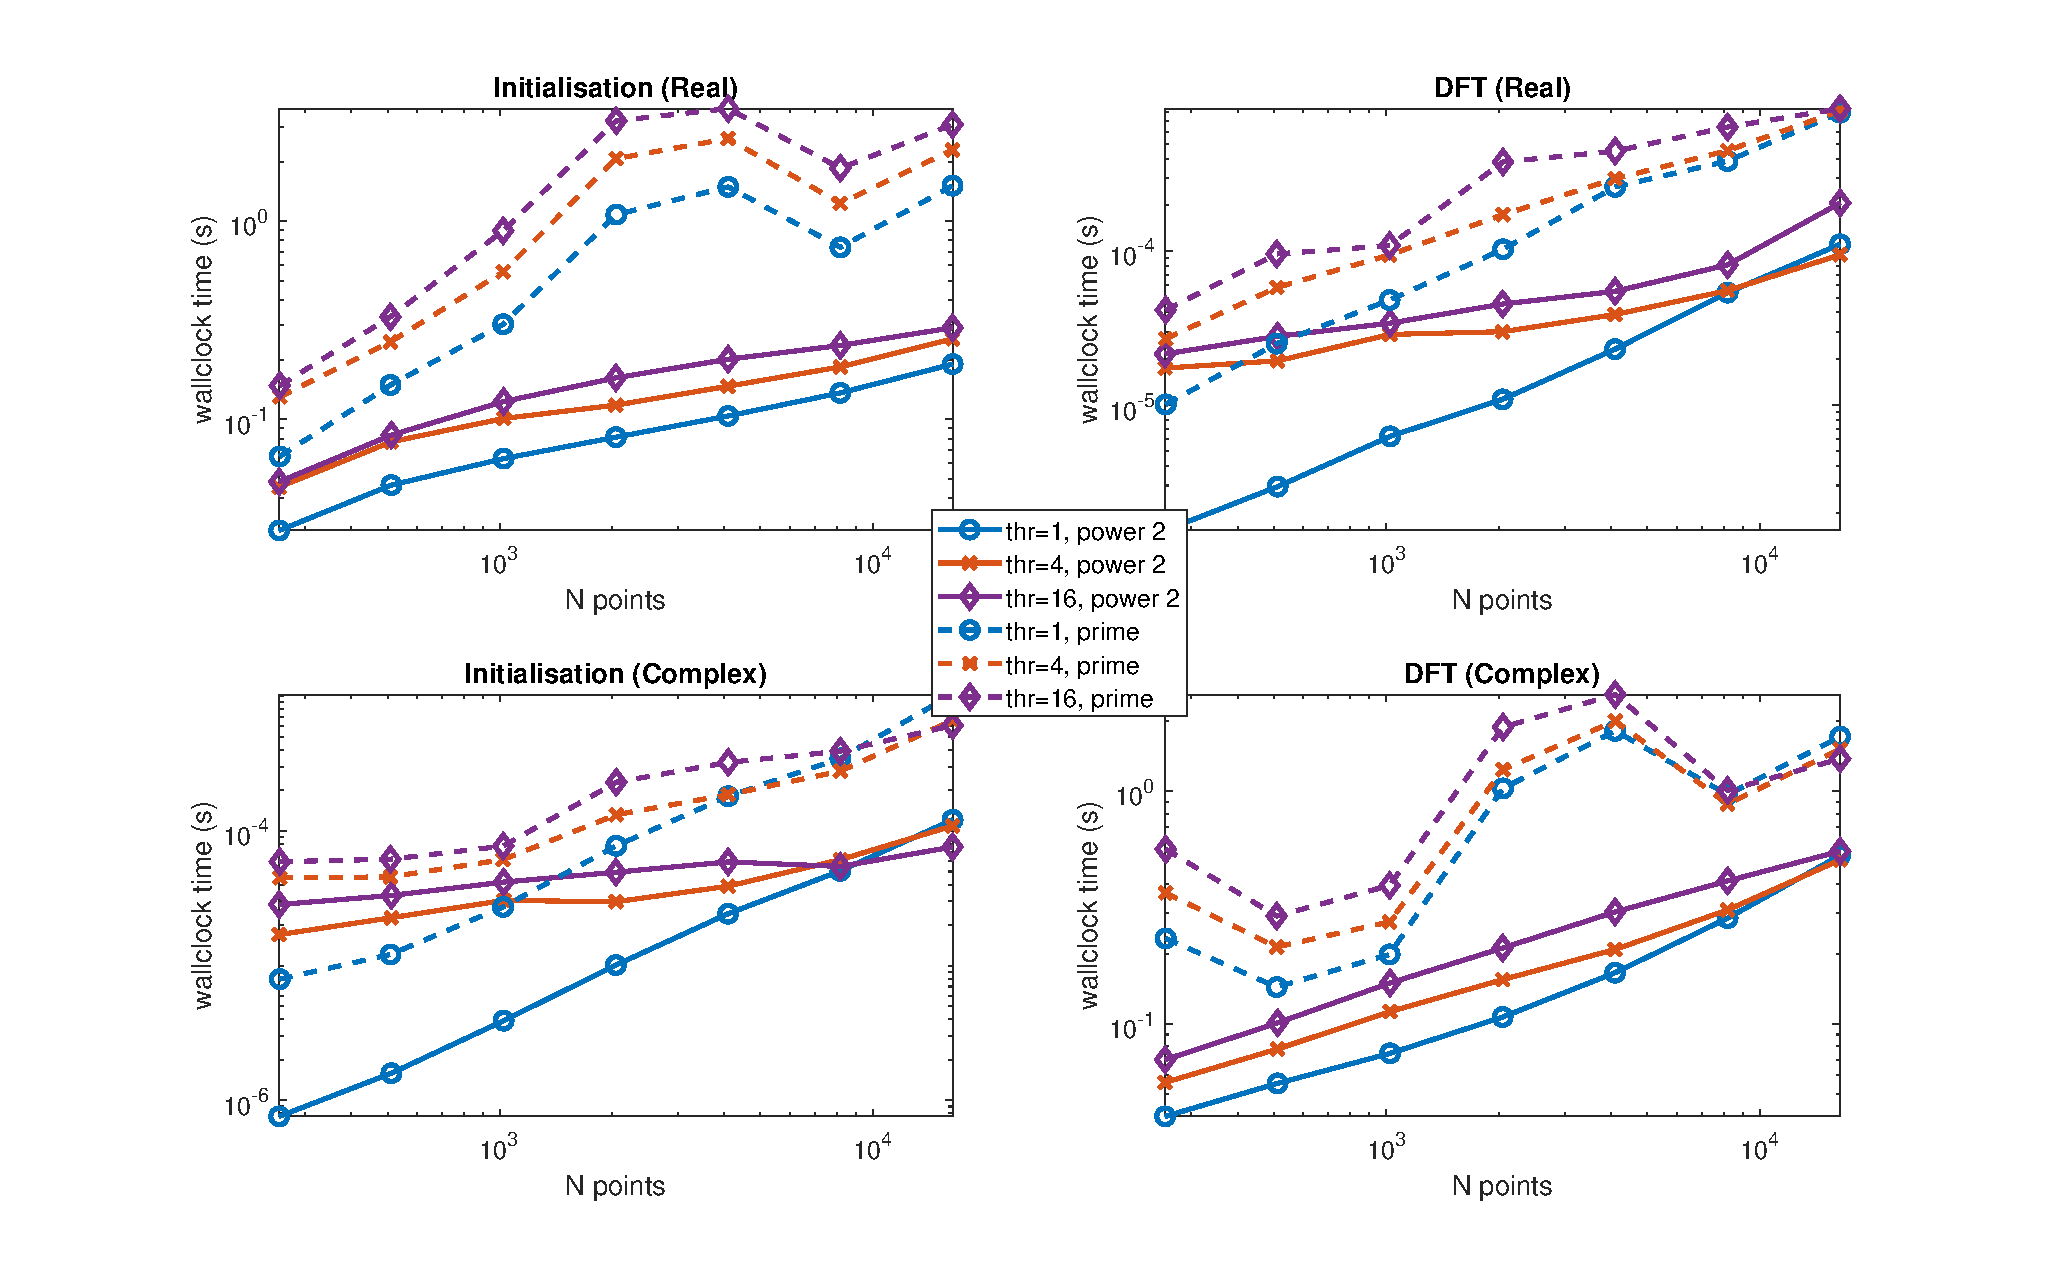
\includegraphics[width=0.9\linewidth]{../results/fftw_1d_thr.eps}
  \caption{Initialisation and DFT execution times of FFTW library applied to 1D signal as a function of the
    number of points, $N,$ and varying the number of threads, $thr.$ }
  \label{fig:1DFFTW}
\end{figure}

To further understand the results, we provide Table~\ref{Tbl:FFTW1d}
(Appendix~\ref{App:1Dthr}), which provides the (wall clock) execution
times of the initialisation stage and the DFT calculations along with
their ratio with respect to one thread for $thr=1,$ 2, 4, 8, 12, 16
and 24. Results for both real and complex input signals are given for
$N=2048,$ 2053, 16381 and 16384.

For $N=2048$ and $N=2053$ with real input signals, we start by
noting that both the initialisation and DFT times tend to increase as
the number of threads increases. This is not unsurprising because they
are very small problems. The
initialisation times are between 13.2 and 19.8 times larger when $N$
is prime compared to $N$ being a power of 2 ($thr=1$ had the smallest
ratio); the DFT computation times are 5.5 and 11.5 times larger for
the prime value of $N$ compare with $N$ being a power of 2 (the
smallest ratio was for $thr=8$). For $N=2048,$ the initialisation time
is between 3400 and 7500 times larger than the average time to perform
one DFT: in general, the ratio decreased as the number of threads
increased. When $N=2053,$ the initialisation time was between 5300 and
14250 times larger than the average DFT time with the lower ratios
occuring for the larger values of $thr.$

For complex-valued signals and $N=2048$ or 2053, increasing the number
of threads also increases the wallclock times. When $N$ is a power of
2 ($N=2048$), the initialisation times are between a factor of 8.0 and
9.6 times smaller than for the nearest prime value of $N;$ the DFT
times are between a factor of 7.7 and 4.4 times smaller. When
$N=2048,$ the initialisation times are between 4290 and 10600 times
larger than the average DFT time; for $N=2053,$ the ratio between
initialisation and DFT times is between 4933 and 13300. In both cases,
the ratio drops as the number of threads increases and, for each value
of $thr,$ the ratio is larger for $N=2053$ than that of $n=2048.$






\subsection{1D MKL Library}\label{Sec:1DMKL}

The 1D MKL library benchmark runs for 1, 4 and 16 threads ($thr$) are compared
in Figure~\ref{1DMKL}. Initialisation times for $N$ a power of 2 are
nearly always lower than when $N$ is a prime number. For a single
thread, the initialisation time increased as the value of $N$
increased but the rate of increase was much larger when $N$ was
prime. For 4 or 16 threads and $N$ a power of 2, the initialisation
time stays almost constant for $N\le 2^{17}$ and then drops: in the
real case, it then starts rising again for the largest values of $N$
considered. When $N$ is a prime value and 4 or 16 threads are used,
the initialisation times remain almost constant for $N\le 2^{14}$ and
then rises with problem size for larger values of $N.$ For the smaller
values of $N,$ the initialisation times is significantly lower when
one thread is used instead of 4 or 16 (a factor of approximately 10
difference).


\begin{figure}[!htb]
    \centering
    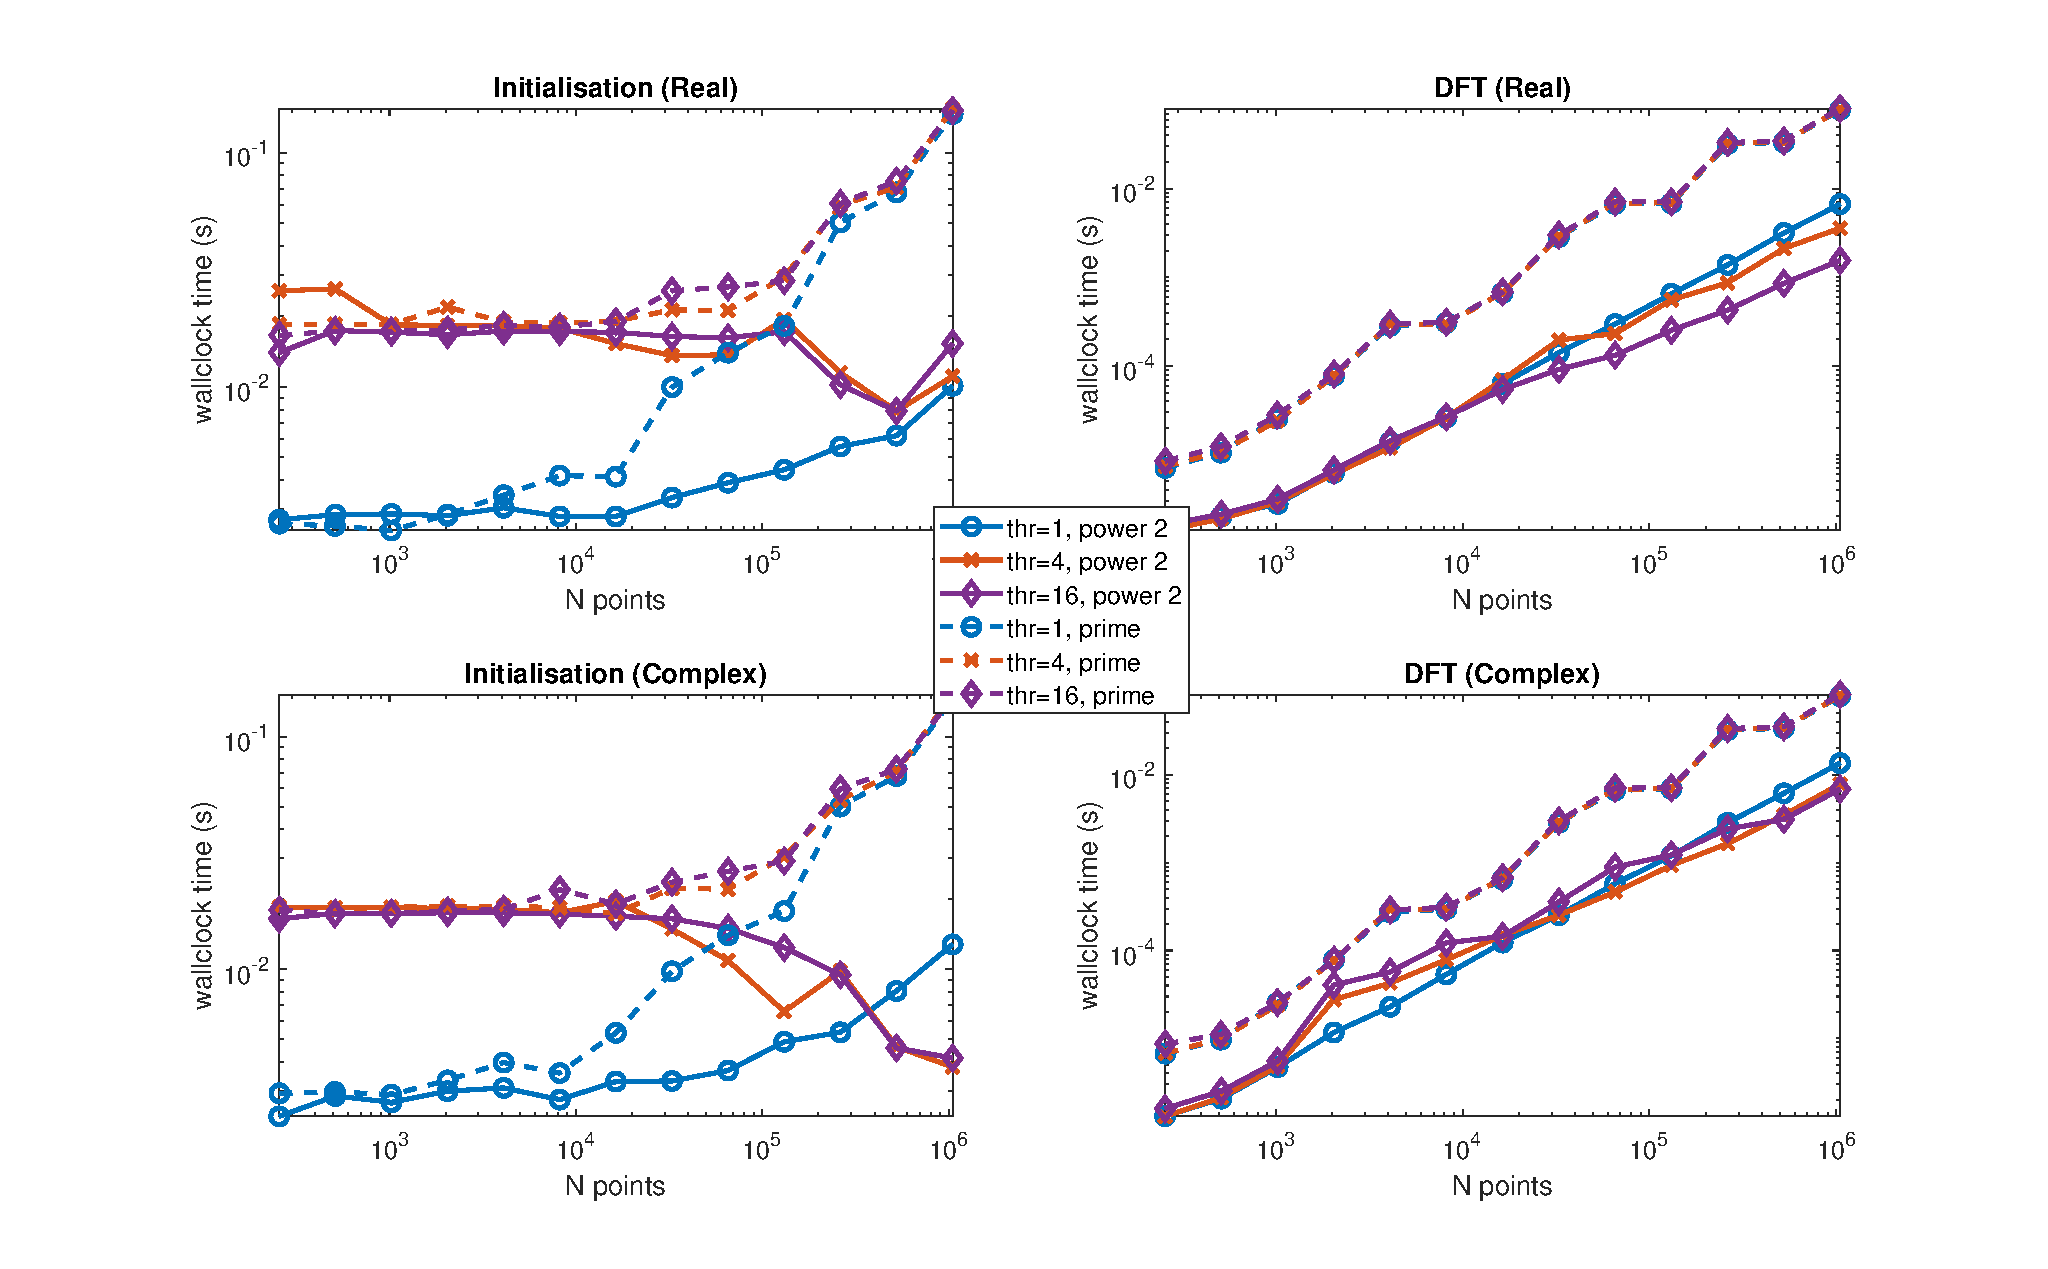
\includegraphics[width=0.9\linewidth]{../results/mkl_1d_thr.eps}
  \caption{Initialisation and DFT execution times of MKL library applied to 1D signal as a function of the
    number of points, $N,$ and varying the number of threads, $thr.$ }
  \label{1DMKL}
\end{figure}

As expected, the DFT times are higher when $N$ is prime compared to
$N$ being a power of 2. There is little effect on the DFT time when
the number of threads is varied but $N$ is prime. However, when $N$ is
a power of 2 and greater than $2^{14}$ (real case) or $2^{17}$
(complex case), there is an advantage to using musing multiple threads
with respect to DFT wallclock time. In Table~\ref{Tbl:MKL1d}
(Appendix~\ref{App:1Dthr}, we provide the (wall clock) execution times
of the initialisation stage and the DFT calculations along with their
ratio with respect to one thread for $thr=1,$ 2, 4, 8, 12, 16 and
24. Results for both real and complex input signals are given for
$N=2048,$ 2053, 16381, 16384, 1048573 and 1048576. We observe that
when $N$ is prime, there is little difference between the real and
complex results. The DFT time is almost unchanged when the number of
threads is increased but the initialisation time increases
significantly for the two smaller values of $N$ in the
table. Additionally, the initialisation times are between two and
three orders of magnitude larger than the DFT times for $N=2053$ and
16381. For the largest prime value of $N$ considered, increasing the
number or threads increases the DFT time very slightly (upto 6\%
increase for 24 threads) and also results in a slight increase in
initialisation time (upto 10\%), with the initialisation time being
roughly 90\% greater than the DFT time.

For the values of $N$ that are powers of 2, the table shows that
increasing the number of threads does, in general, result in an
increase in initialisation time and for the smaller values of $N$ the
initialisation time can increase by a factor of almost 10 (real) or 6
(complex): given that there is little difference in DFT time for
differing numbers of threads, we do not advocate using multiple
threads for these smaller values of $N.$ For $N=1048576$ increasing
the number of threads from a single thread results in at most an
increase of 79\% (real) or 32\% (complex) in initialisation time. For
the real case, 16 threads reduces the DFT time by a factor of ~4 and,
for the complex case, the DFT time is reduced by a factor of
~2.4. Given that the initialisation and DFT times are at most a factor
of 10 different, only a small number of DFT computations are required
to overcome the increase in initialisation time.








\subsection{Comparison of libraries for 1D benchmarks}\label{Sec:1DComp}

In Figure~\ref{1DFFTWMKL2}, we compare the 1D FFTW and MKL libraries
with multithreading for values of $N$ that are powers of 2. Our
first observation is that, in our computing environment, the MKL
library can perform DFT computations for larger values of $N.$ For the
values of $N$ where we can compare the libraries, MKL has
significantly lower initialisation times. For DFT times, in the real
case, MKL is always faster than FFTW but in the complex case, the MKL
library is best for the very small values of $N$ but as we approach
$N=16384,$ the times appear to be similar. Given the substantial
difference in initialisation time and the larger values of $N$
available for use by the user, we recommend that the MKL library is
used.



\begin{figure}[!htb]
    \centering
    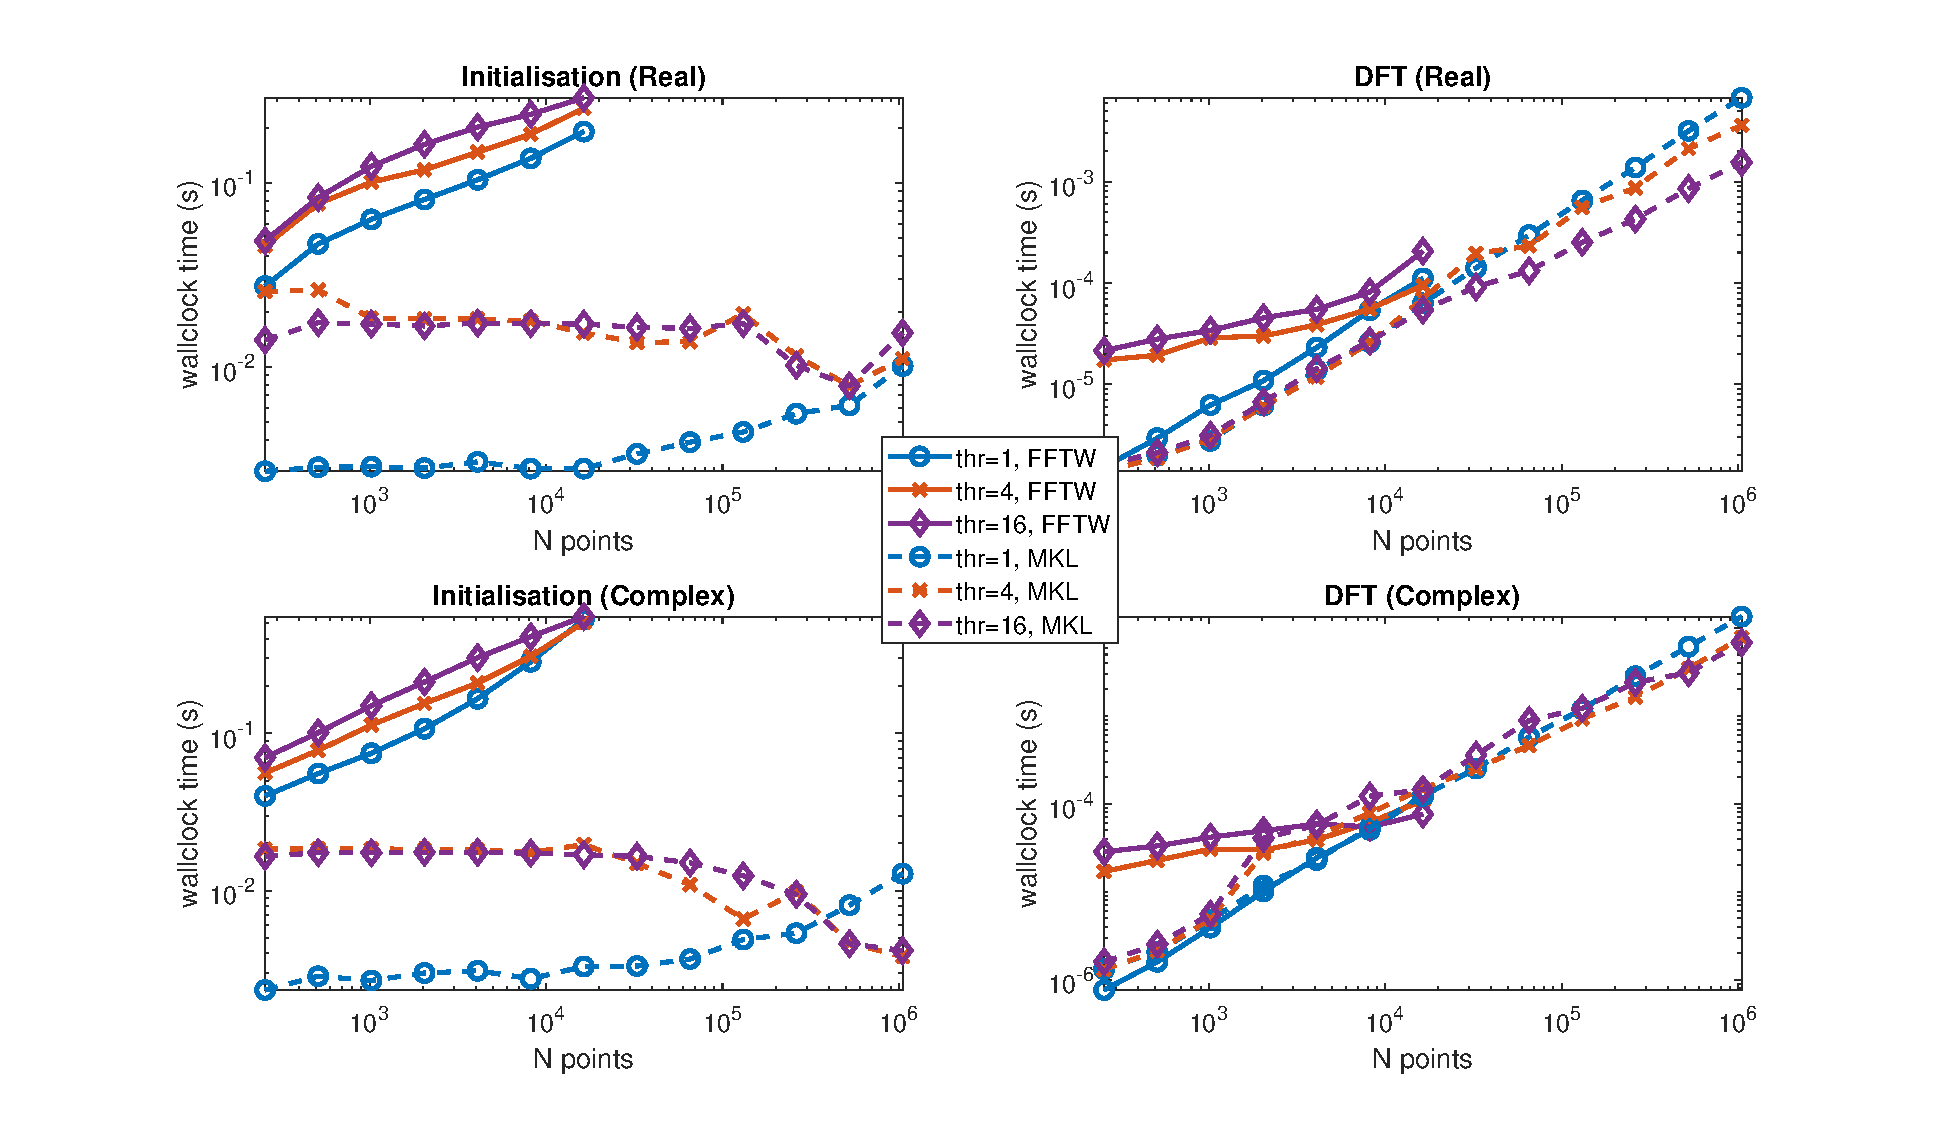
\includegraphics[width=0.9\linewidth]{../results/fftw_mkl_2_1d_thr.eps}
  \caption{Initialisation and DFT execution times of FFTW and MKL libraries applied to 1D signal as a function of the
    number of points, $N,$ and varying the number of threads, $thr.$ $N$ is a power of 2.}
  \label{1DFFTWMKL2}
\end{figure}



The FFTW and MKL libraries are compared in Figure~\ref{1DFFTWMKLPrime}
for prime values of $N.$ As with the case when $N$ is a power of 2,
the initialisation times are significantly lower for the MKL
library. The difference in DFT times is not as pronounced as in the
former case but MKL is still generally faster than FFTW (although, if
the library could accommodate larger values of $N,$ FFTW looks like it
would be faster for these values). Therefore, when $N$ is a prime
number, we recommend using the MKL library over the FFTW library.

\begin{figure}[!htb]
    \centering
    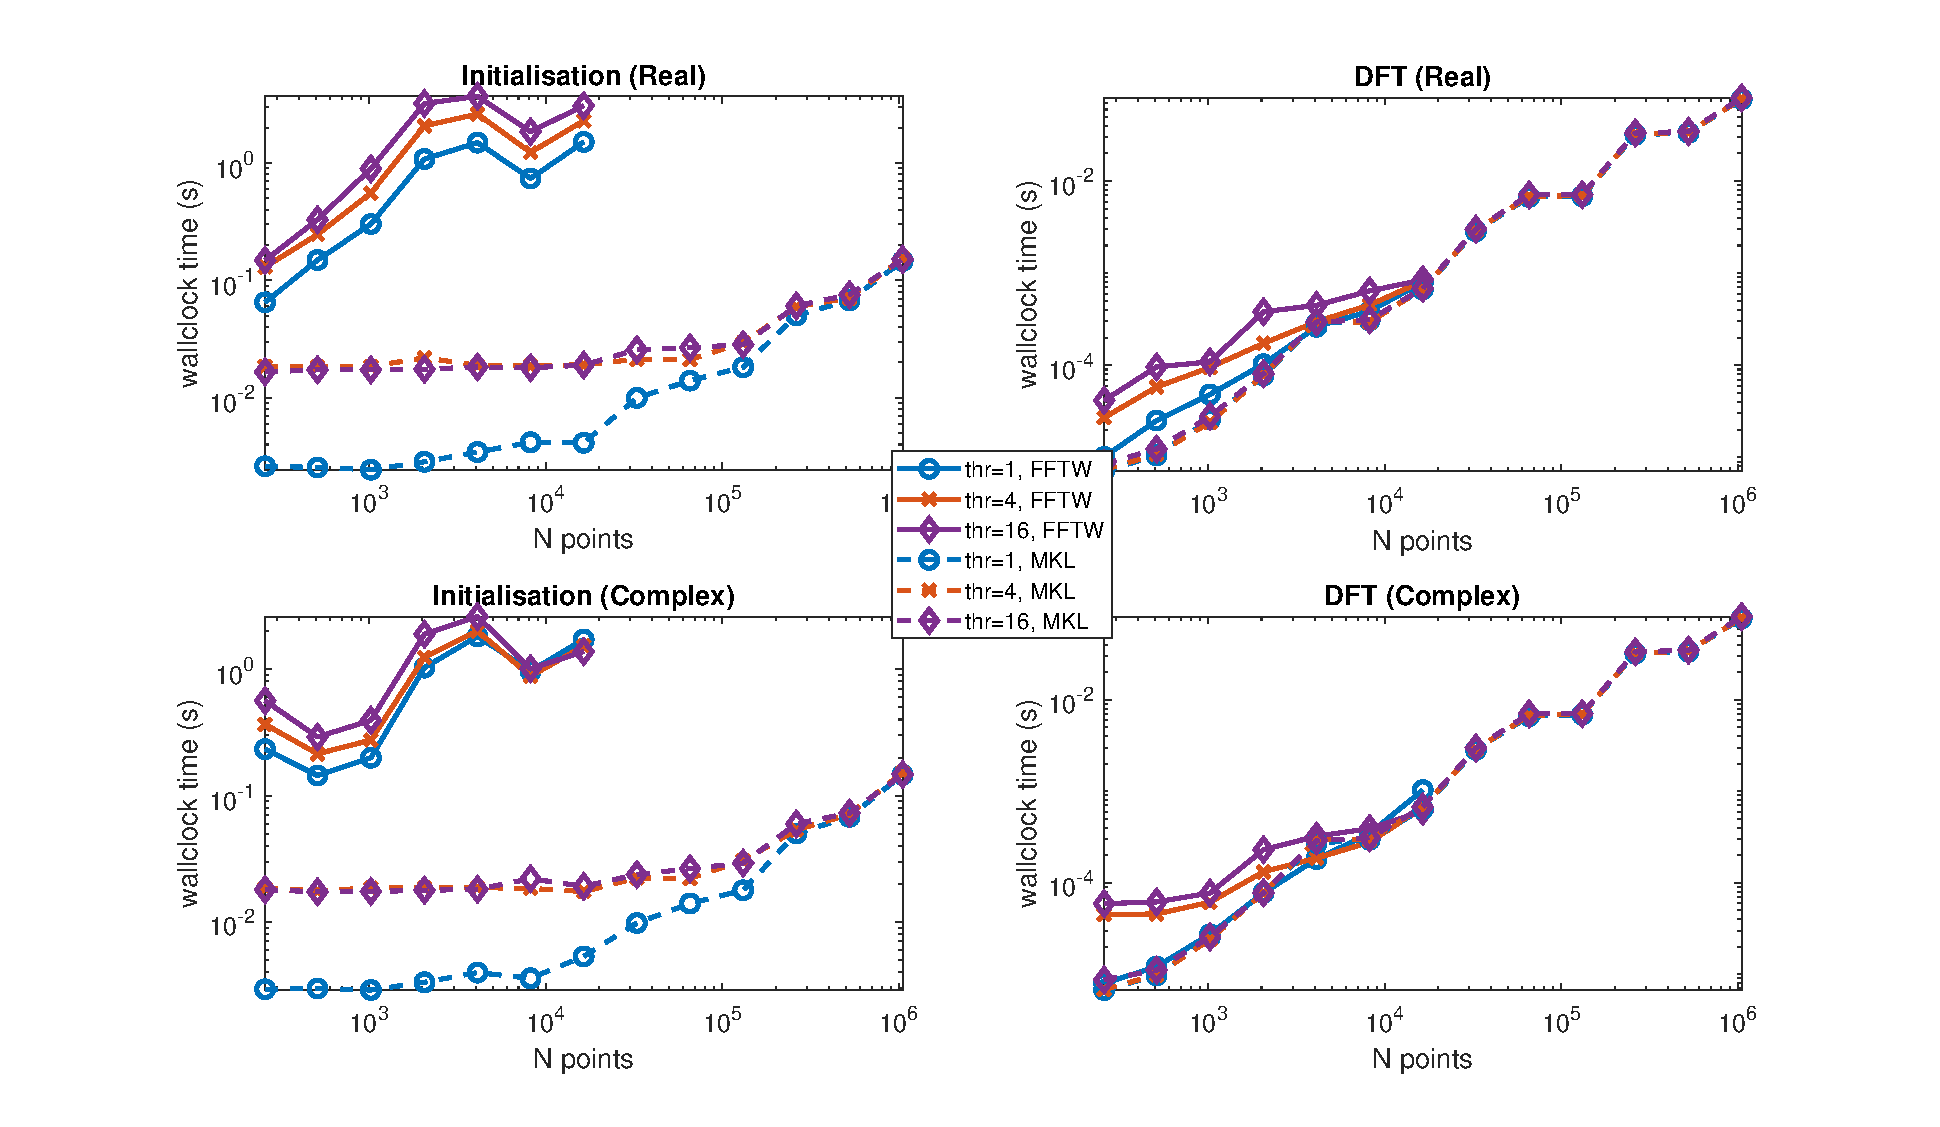
\includegraphics[width=0.9\linewidth]{../results/fftw_mkl_prime_1d_thr.eps}
  \caption{Initialisation and DFT execution times of FFTW and MKL libraries applied to 1D signal as a function of the
    number of points, $N,$ and varying the number of threads, $thr.$ $N$ is a prime number.}
  \label{1DFFTWMKLPrime}
\end{figure}


\section{Effect of domain size and multithreading for 2D benchmarks}\label{Sec:2DMulti}
The benchmark results for libraries that perfrom the fast Fourier
transform over a 2D domain are discussed in this section. As with the
1D results in Section~\ref{Sec:1DMulti}, the P3DFFT library cannot be
used on these problems so we compare the OpenMP versions of the FFTW
and MKL libraries.

Similarly to the benchmarks in Section~\ref{Sec:1DMulti}, we set
$n_3=4,$ $n_q=4$ and $n_1=n_2=N,$ were $N$ is defined as follows.  For one
set of tests, we let $N=2^k$ for $k=5,\ldots,12.$ For the other set of
tests, $N$ is defined to be the closest prime number to $2^k,$
$k=5,\ldots,12:$ if two primes are equidistant, we choose the larger
one.

\subsection{2D FFTW Library}\label{Sec:2DFFTW}

In Figure~\ref{2DFFTW}, we compare our single node benchmark
experiments for the multithreaded FFTW library for 1, 4 and 16 OpenMP
threads. There is a difference in behaviour between the real and
complex benchmarks. For $N$ smaller than 200, the initialisation times
for the real case are smaller when $N$ is prime compared to when $N$
is a power of 2; for the complex case, the initialisation times for
$N$ prime are, in general, greater than $N$ a power of 2. For larger
values of $N,$ the initialisation times for prime values of $N$ are
larger than $N$ a power of 2 in both the real and complex cases but
the complex initialisation times appear to be higher than in the real
case. Increasing the number of threads also increases the
initialisation times but, as the problem size increases, the
difference between 4 and 16 threads generally diminishes. For further
clarity of the benchmark results, we provide the (wall clock)
execution times of the initialisation stage and the DFT calculations
along with their ratio with respect to one thread for $thr=1,$ 2, 4,
8, 12, 16 and 24 in Tables~\ref{Tbl:FFTW2d} and
\ref{Tbl:FFTW2dc} (Appendix~\ref{App:2Dthr}). Results for both real and complex input signals are
given for $N=31,$ 32, 256, 257, 2048 and 2053. These confirm that the
initialisation times are lower for the real case compared to the
complex case. Additionally, increasing the number of threads has less
of an effect when $N$ is prime compared to when $N$ is a power of
2. However,

Comparing the DFT times in Figure~\ref{2DFFTW}, for the larger values
of $N,$ increasing the number of threads is always improving the
wallclock time. When $N$ is a power of 2, a single thread is
prefereable for $N\le 128.$ The DFT times are larger when $N$ is a
prime number instead of being a power of 2. Using
Tables~\ref{Tbl:FFTW2d} and \ref{Tbl:FFTW2dc}, we see observe that
increasing the number of threads results in lower ratios when $N$ is a
prime compared to when $N$ is a power of 2. Given that the
initialisation times are at least one order of magnitude larger than
the DFT times, when a small number of DFT calculations are being
performed with a single initialisation, it is normally best to use a
single thread when $N$ is small (less than 300) but for a large value
of $N$ we recommend using 16 or 24 threads (the latter if performing a
large number of DFT calculations).




\begin{figure}[htb]
    \centering
    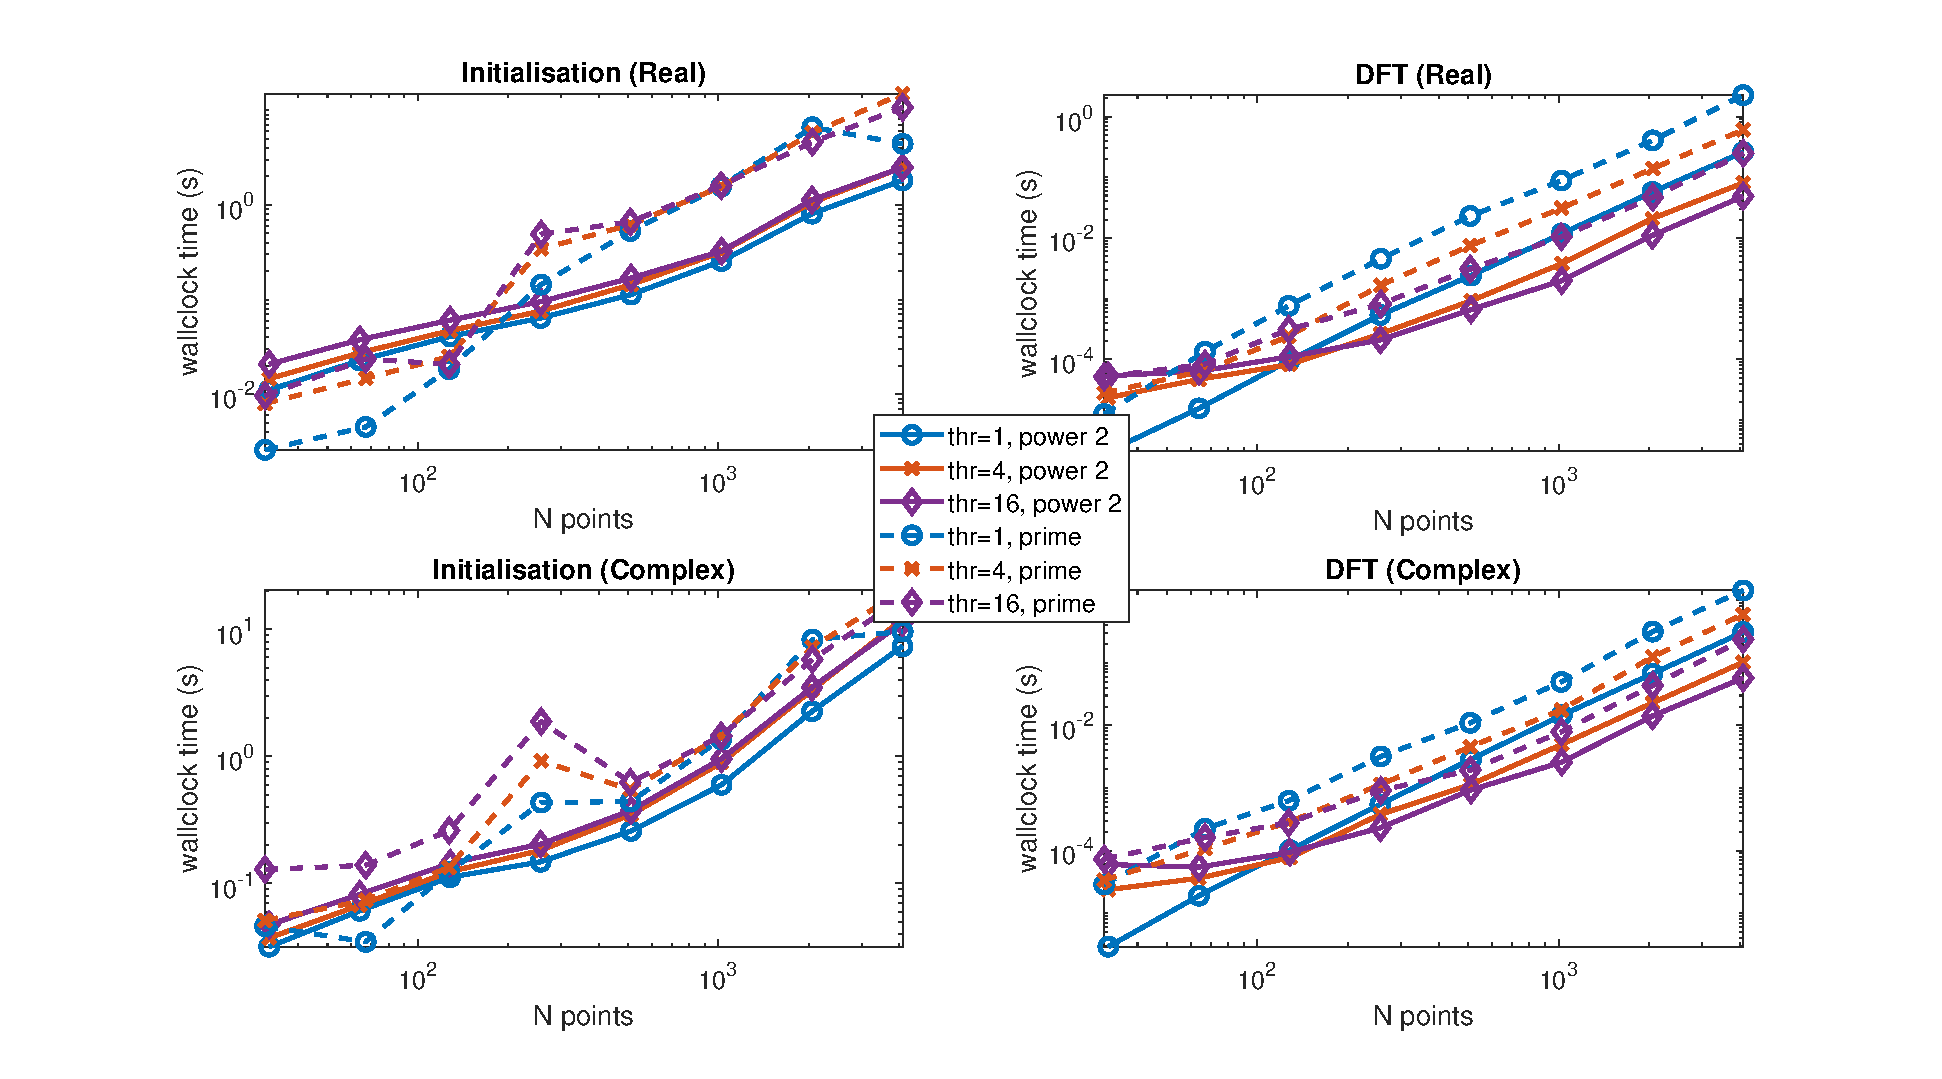
\includegraphics[width=0.9\linewidth]{../results/fftw_2d_thr.eps}
  \caption{Initialisation and DFT execution times of FFTW library applied to 2D signal as a function of the
    number of points, $N,$ and varying the number of threads, $thr.$ }
  \label{2DFFTW}
\end{figure}



\subsection{2D MKL Library}\label{Sec:2DMKL}

In Figure~\ref{2DMKL} we do the same comparisions as in
Figure~\ref{2DFFTW} but for the MKL library. For a single thread, when
$N$ is lower than 600, the initialisation times remain roughly
constant as $N$ increases and, once $N$ is greater than 600, the
initialisation time increases but at a faster rate for real signal
inputs. When mulitple threads are used, the initialisation time is
initially high but starts to decrease as $N$ increases. For 16
threads, this decrease starts sooner when the input signal is complex
and, once $N$ is greater than 1000, the multiple threads leads to
smaller initialisation times than when a signal thread is used; in the
real case, the multithreads have improved initialisation times for
$N>2000.$ In general, there is little difference between $N$ being
prime and a power of 2 for one or 16 threads with real input signals
although, for the larger values of $N$, the initialisation time is
better when $N$ is a power of 2. For complex input signals, switching
between $N$ being a power of two and $N$ being prime has little effect
on the initialisation time when one or four threads is used. For the
larger problem sizes, increasing the number of threads has a positive
affect on the initialisation time.  This is confirmed in
Table~\ref{Tbl:MKL2d}, where we see that the initialisation time is
roughly halved when 24 threads are used compared to a single thread.



\begin{figure}[htb]
    \centering
    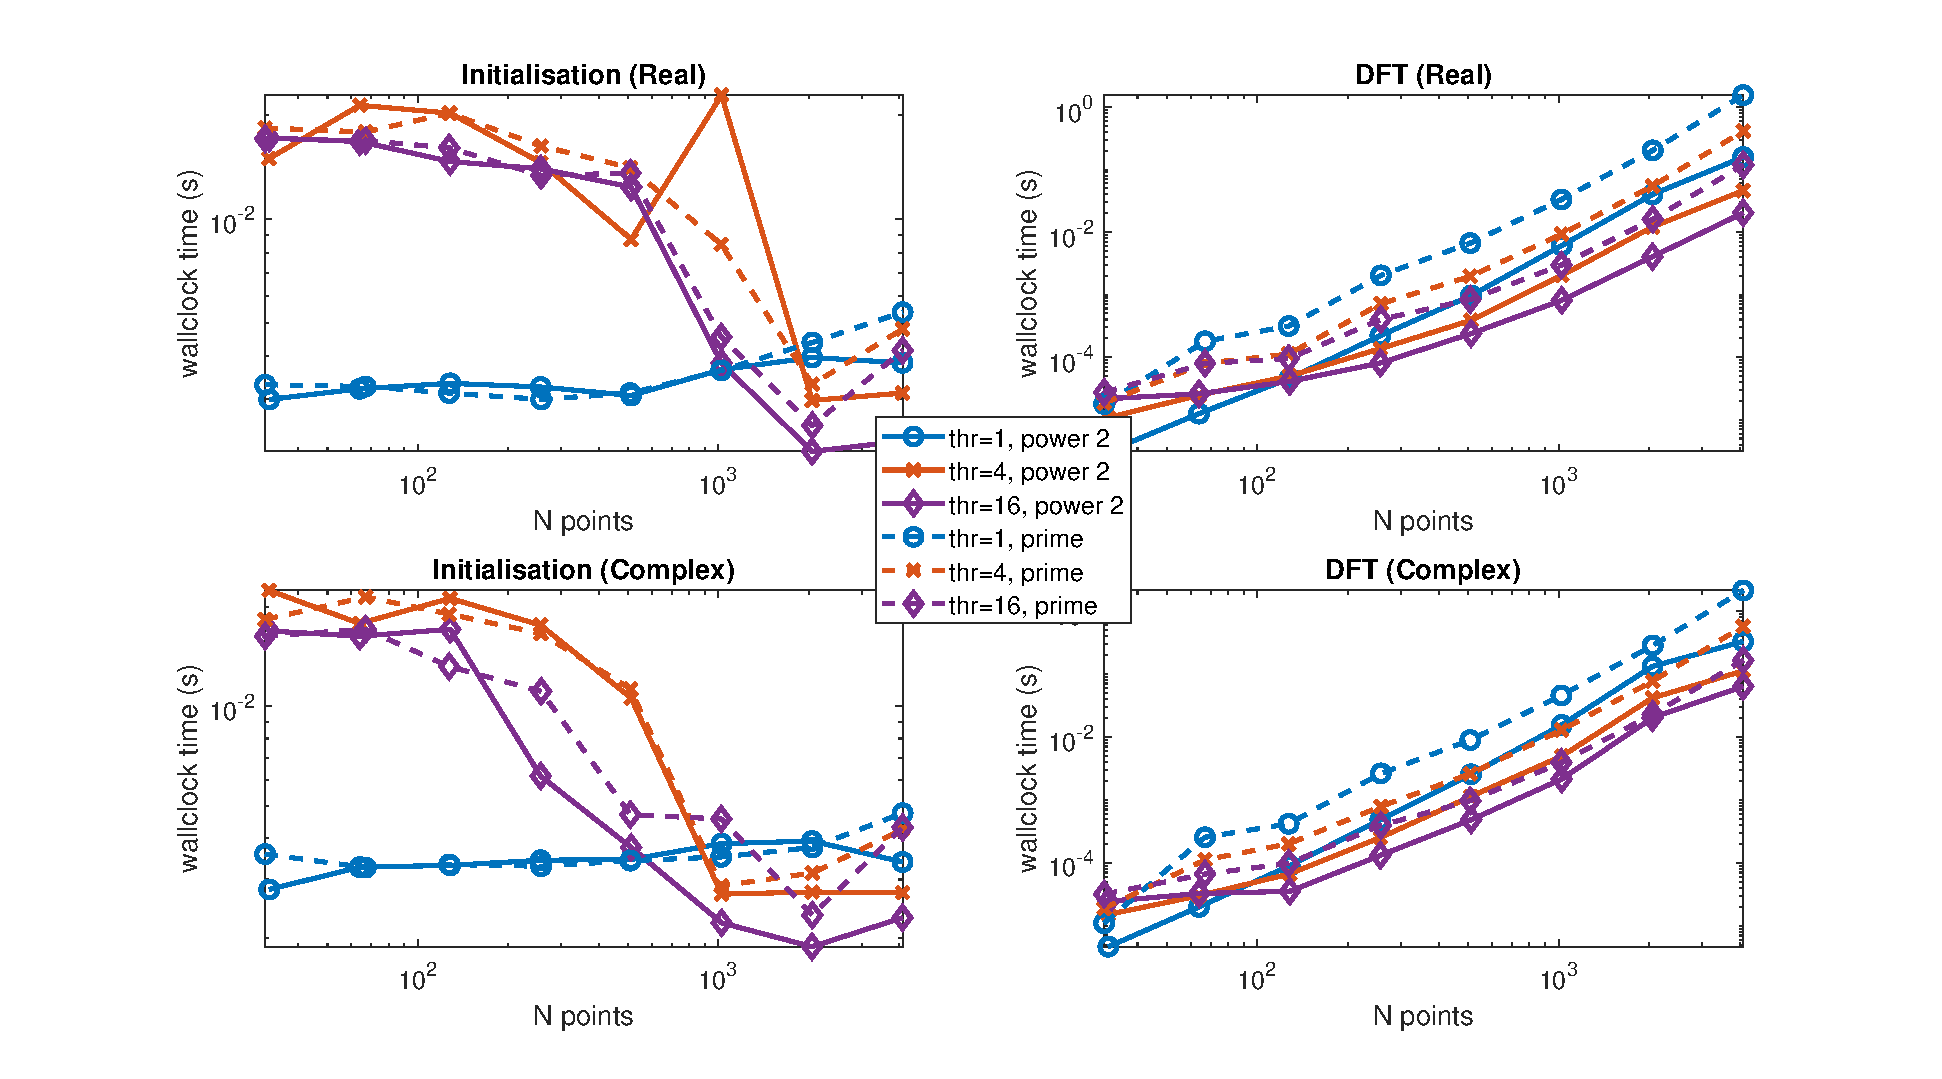
\includegraphics[width=0.9\linewidth]{../results/mkl_2d_thr.eps}
  \caption{Initialisation and DFT execution times of MKL library applied to 2D signal as a function of the
    number of points, $N,$ and varying the number of threads, $thr.$ }
  \label{2DMKL}
\end{figure}




As expected, in Figure~\ref{2DMKL} we observe that increasing the
problem size increases the DFT calculation time. Except for the very
smallest value of $N,$ where $N$ is prime, increasing the number of
threads from 1 to 4 to 16 produces monotonic reductions in the DFT
time in both the real and complex cases. For $N$ a power of 2 and
smaller than 256 (real case) or 128 (complex case), using multiple
threads increases the DFT time. For larger values of $N,$ multiple
threads decreases the DFT times. This is confirmed in
Table~\ref{Tbl:MKL2d} but we see that there is little gain with
respect to DFT time in going above 12 threads. However, the additional
reduction in initialisation time for using more than 12 threads for
large values of $N$ leads us to conclude that, on a single node of
ARCHER, it is advantageous to use all the threads available when $N$
is greater than 2000 (real case or complex case with $N$ prime) or
1000 (complex case with $N$ a power of 3). For $N=256,$ we can work
out the number of DFT calculations, $k,$ that would be required for
$thr$ threads to have a lower time than a single thread when
performing a single initialisation and $k$ DFT calculations. We
provide this information in Table~\ref{Tbl:MKL2dk} and observe that
multithreading can be positively utilised for lower values of $k$ when
$N$ was prime because of the greater time to perform a DFT calculation
(a factor of 4-5 difference) but the initialisation times are, in
general, similar. Additionally, the complex case also requires smaller
values of $k$ compared to the real case.



\begin{table}
\begin{center}
%\being{small}
\begin{tabular}{|r||r|r||r|r|}
  \hline
 & \multicolumn{2}{|c||}{$k(N=256)$} & \multicolumn{2}{|c|}{$k(N=257)$} \\
$thr$ &  Real & Complex &  Real & Complex  \\ \hline
  2 & 49 & 0   &  1 & 2 \\
  4 & 135 & 62 & 11 & 8 \\
  8 & 70 & 42 & 12 & 8 \\
  12 & 86 & 29 & 11 & 3 \\
  16 & 77 & 8  & 7 & 4 \\
  24 & 83 & 31 &10 & 6  \\ \hline
\end{tabular}
\caption{ For $N=256$ and $N=257,$ the number of DFT calculations, $k,$ required for $thr$ threads to have a lower wallclock time than a single thread when performing  a single initialisation and $k$ DFT calculations are performed with the 2D interface to the FFTW library.  }\label{Tbl:MKL2dk}
%\end{small}
\end{center}
\end{table}

\subsection{Comparison of libraries for 2D benchmarks}\label{Sec:2DComp}

In Figure~\ref{2DFFTWMKL2}, we compare the initialisation and DFT
wallclock times for the FFTW and MKL libraries with our 2D benchmark
runs for $N$ a power of 2. For the real case, there is a stark
difference in initialisation times as $N$ grows with MKL being faster:
when $N=4096$ the FFTW time is a factor of 475 larger than that of MKL
when a single thread is used; for $thr=4,$ the factor is 800; and for
$thr=24,$ factor is 1500. Looking at Figure~\ref{2DFFTWMKL2}, the
complex case appears to have similar differences in initialisation
times but for $N=4096,$ the factors are 2170, 4380 and 3350 for
$thr=1,$ 4 and 24, respectively. Additionally, the MKL DFT wallclock
times are lower than those of FFTW (real case) or, in general, very
similar for the complex case. Thus, when $N$ is a power of 2, we
recommend using the MKL library.


\begin{figure}[htb]
    \centering
    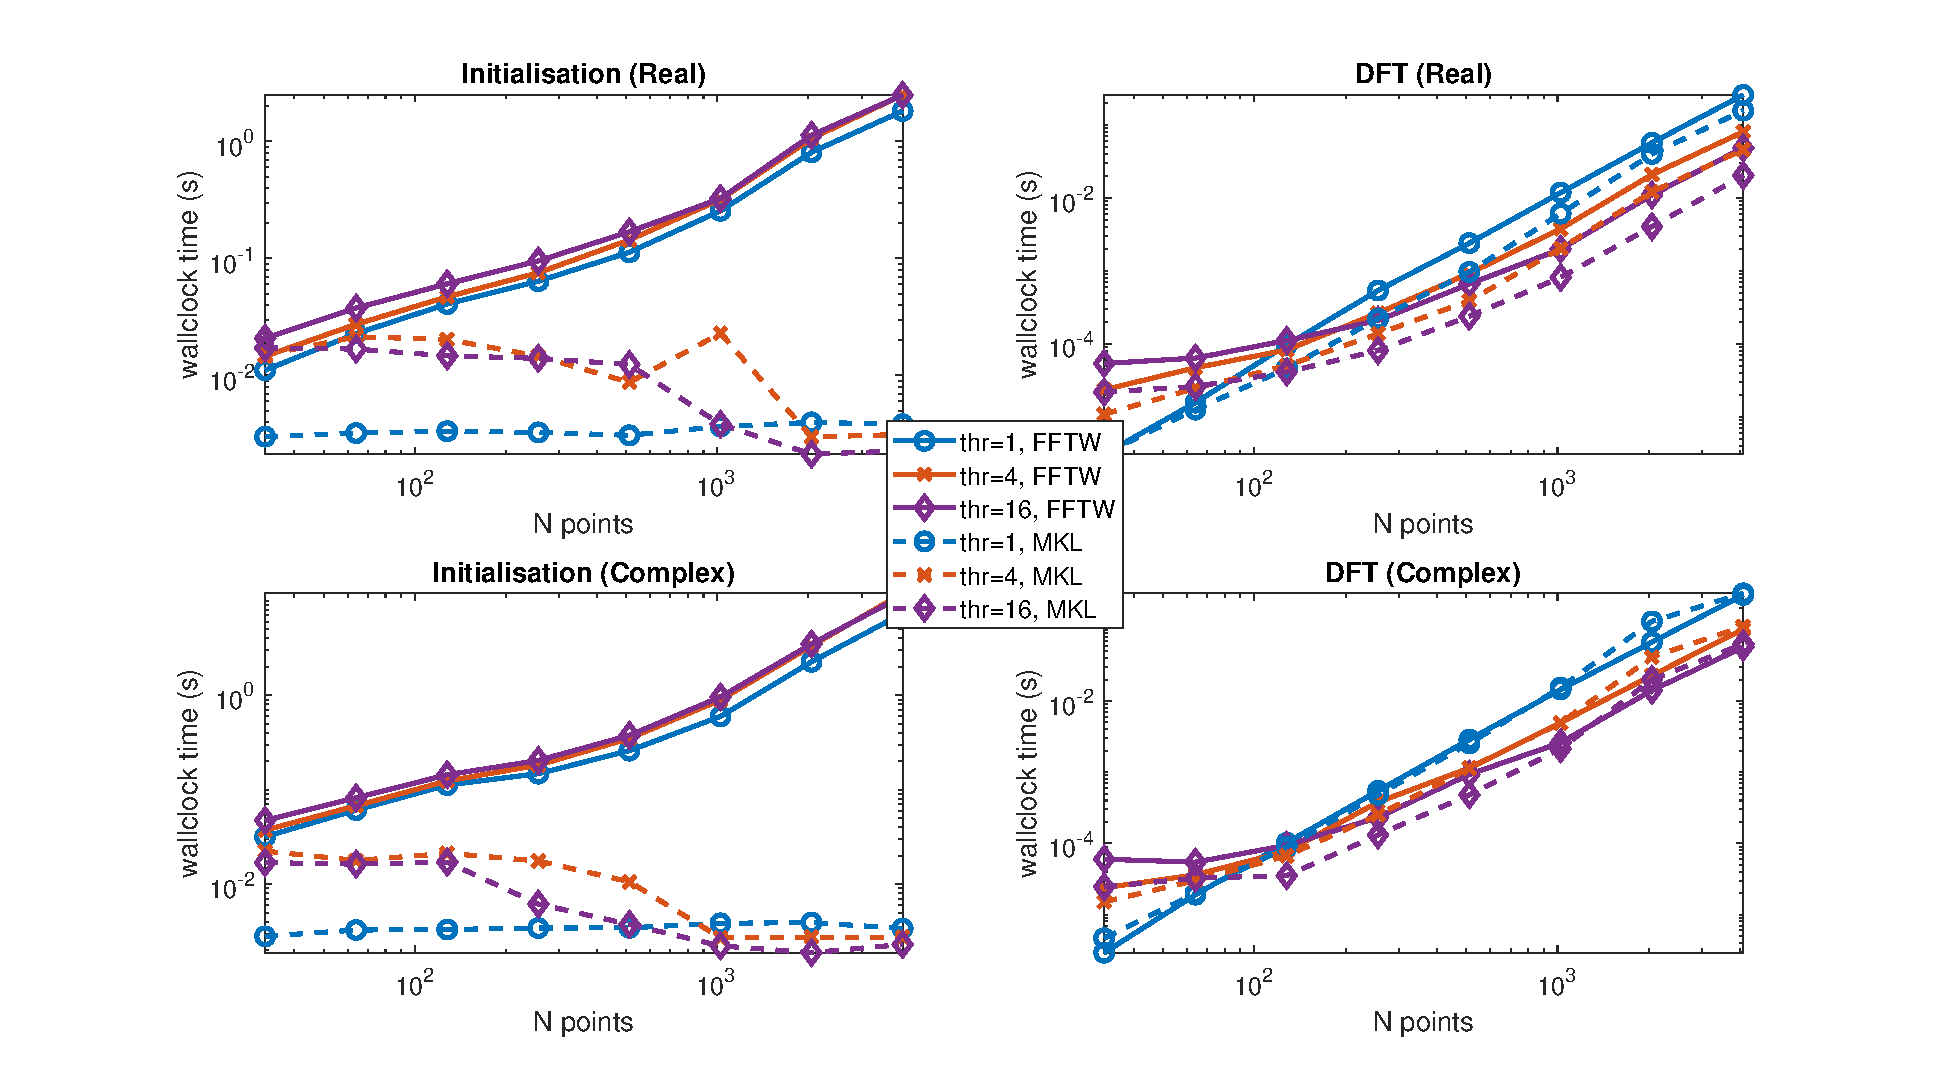
\includegraphics[width=0.9\linewidth]{../results/fftw_mkl_2_2d_thr.eps}
  \caption{Initialisation and DFT execution times of FFTW and MKL libraries applied to 2D signal as a function of the
    number of points, $N,$ and varying the number of threads, $thr.$ $N$ is a power of 2.}
  \label{2DFFTWMKL2}
\end{figure}


We compare the FFTW and MKL library initialisation and DFT times for
prime values of $N$ in Figure~\ref{2DFFTWMKLPrime}. As with the case
when $N$ is a power of 2, there is a marked difference in
initialisation time for large values of $N$ with the MKL library have
significantly lower times. For $N=4099$ with $thr=1,$ 4 and 24, the
difference in initialisation time is a factor of 820, 3120 and 1920,
respectively, for the real case, and 2010, 4750 and 5360,
respectively. In general, the DFT times are slightly better for the
MKL library in both the real and complex cases and, hence, we
recommend using the MKL library.

\begin{figure}[htb]
    \centering
    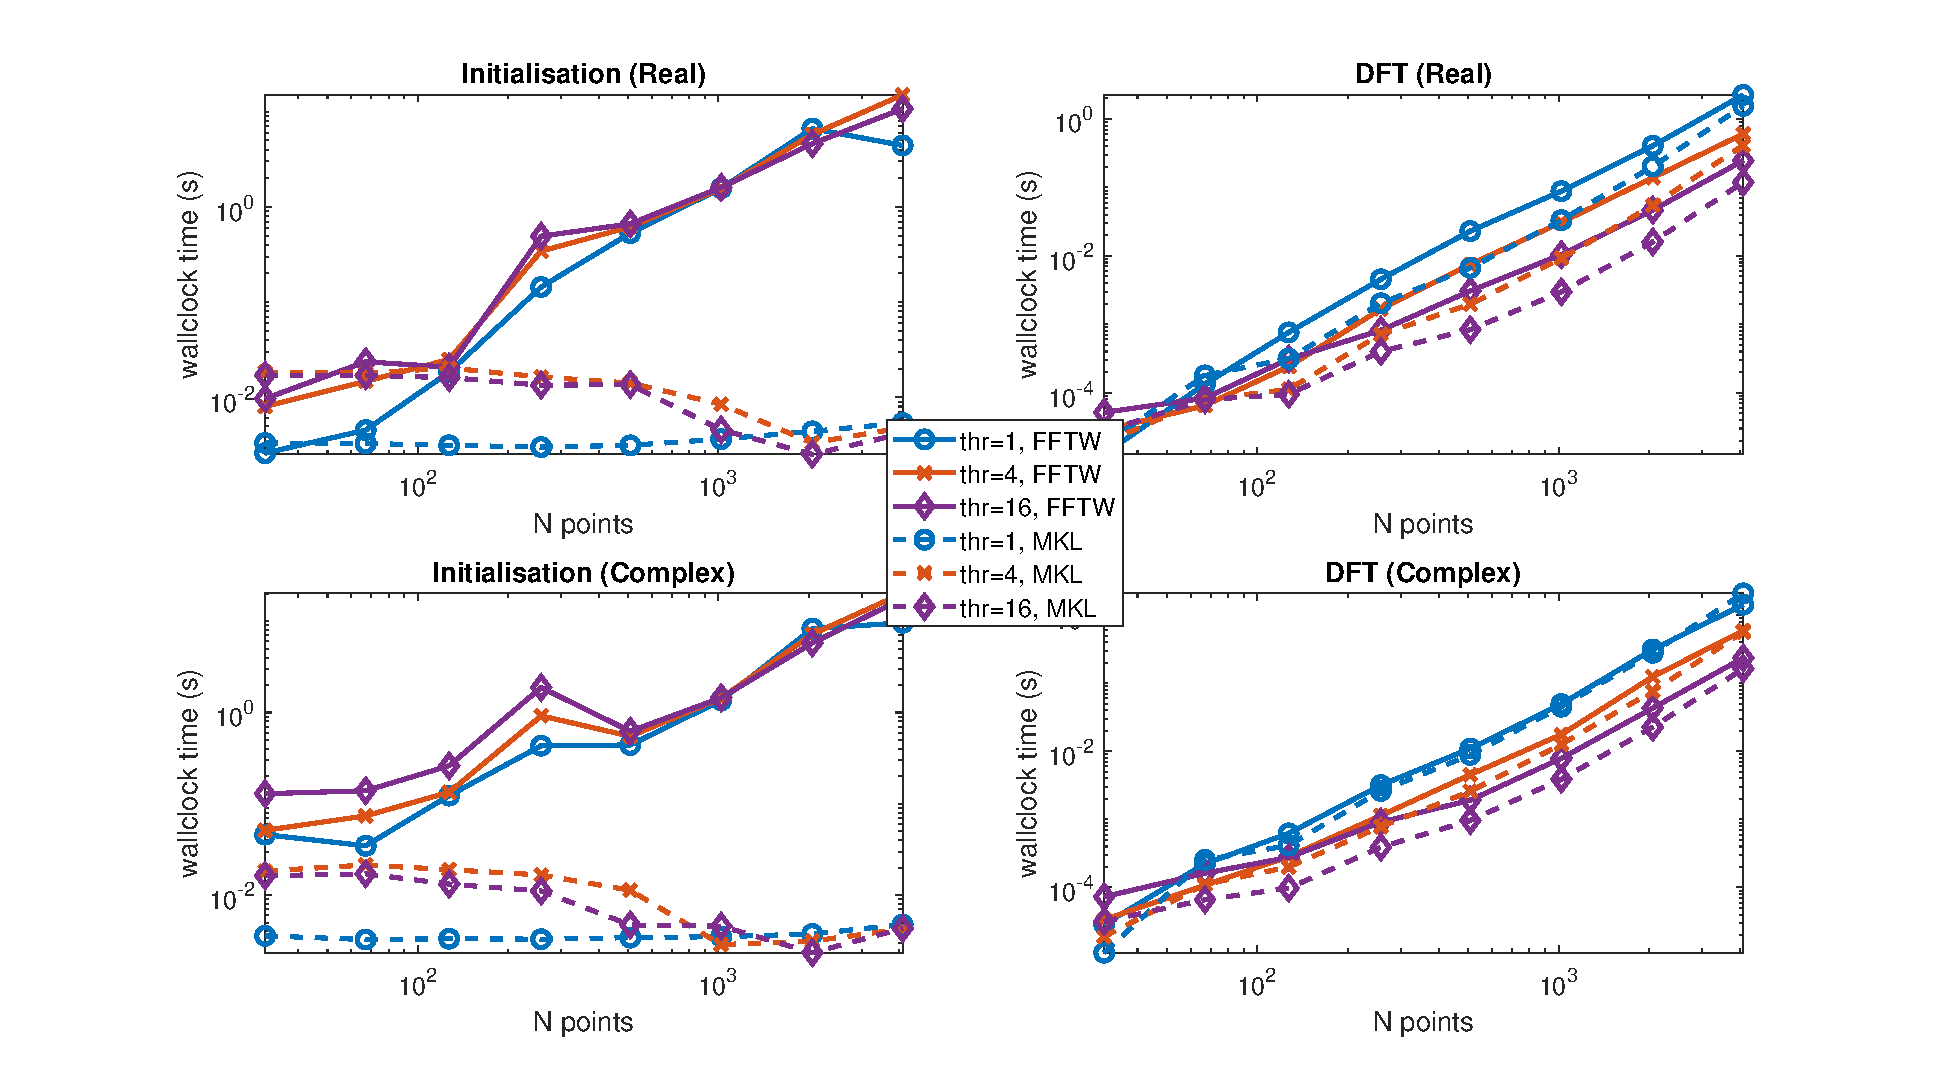
\includegraphics[width=0.9\linewidth]{../results/fftw_mkl_prime_2d_thr.eps}
  \caption{Initialisation and DFT execution times of FFTW and MKL libraries applied to 2D signal as a function of the
    number of points, $N,$ and varying the number of threads, $thr.$ $N$ is a prime number.}
  \label{2DFFTWMKLPrime}
\end{figure}





\section{Effect of domain size and multithreading for 3D benchmarks}\label{Sec:3DMulti}
The results for libraries that perform the fast Fourier transform over
a 3D domain are discussed in this section. The P3DFFT library only
provides a version with both MPI and OpenMP provision and, hence, we
use this version of the library but set the number of MPI processes to
one.

Similarly to the benchmarks in Section~\ref{Sec:1DMulti} and \ref{Sec:2DMulti}, we set
$n_q=4$ and $n_1=n_2=n_3=N,$ were $N$ is defined as follows.  For one
set of tests, we let $N=2^k$ for $k=3,\ldots,9.$ For the other set of
tests, $N$ is defined to be the closest prime number to $2^k,$
$k=3,\ldots,9:$ if two primes are equidistant, we choose the larger
one.

\subsection{3D FFTW Library}\label{Sec:3DFFTW}
The initialisation and DFT times for the FFTW library applied to the
3D benchmark are compared in Figure~\ref{3DFFTW} for 1, 4 and 16
threads. Initialisation times for a single thread are generally lower
than when 4 or 16 threads are used and, in general, the initialisation
times are slightly higher for prime values of $N$ compared to when
they are a power 2. In both the real and complex cases, when $N$ is a
power of 2, it is better to use a single thread with respect to DFT
calculation time for $N$ smaller than 32 and, when $N$ is larger than
32, we start to see the gains in using multiple threads. When $N$ is
prime, multithreading becomes advantageous for values of $N$ greater
than 31 with respect to DFT times. 

To further analyse the benchmark results, we provide the DFT and
initialisation wall clock times for $N=7,$ 8, 31, 32, 509 and 512 with
1,2,4,8,16 and 24 threads in Tables~\ref{Tbl:FFTW3d} and
\ref{Tbl:FFTW3dc} (Appendix~\ref{App:3Dthr}). When $N=7$ or 8, the use of multiple threads has a
catastrophic affect on the DFT time: 24 threads results in a factor of
62 (real case) or 75 (complex case) increase in DFT time when $N=7$
and a factor 47 (real case) or 82 (complex case) when $N=8;$
additionally, the initialisation times triple in the complex case and
increase by a factor of 5 for the real case. When $N=31,$ increasing
the number of threads results in the DFT wallclock time decreasing but
the initialisation time increases: in Table~\ref{Tbl:FFTW3dk} we
provide the number of DFT calculations, $k,$ (on average) that would
be required for $thr$ threads to have a lower time than a single
thread when performing a single initialisation and $k$ DFT
calculations for $N=31,$ 32, 509 and $N=512.$ For $N=31,$ (on average)
increasing the number of threads is never going to improve the overall
time spent initialising and then performing a DFT when the input is
complex. However, for real input, 83 or more DFTs per initialisation
will see an improvement in wall clock when using 8 threads over using
a single thread. For $N=32,$ hundreds of DFTS per initialisation are
required in the cases where it is possible to outperform a single
thread. With real signals and $N=509,$ it is always advantageous to
use multithreading with the architecture and benchmark set-up that we
used, and 24 threads is optimal on a single node with respect to
wallclock time. For complex input signals with $N=509,$ when 8 or more
threads are used, just 2 or more DFT calculations per initialisation
will see a saving in overall wallclock time over using a single
thread.

\begin{figure}[htb]
    \centering
    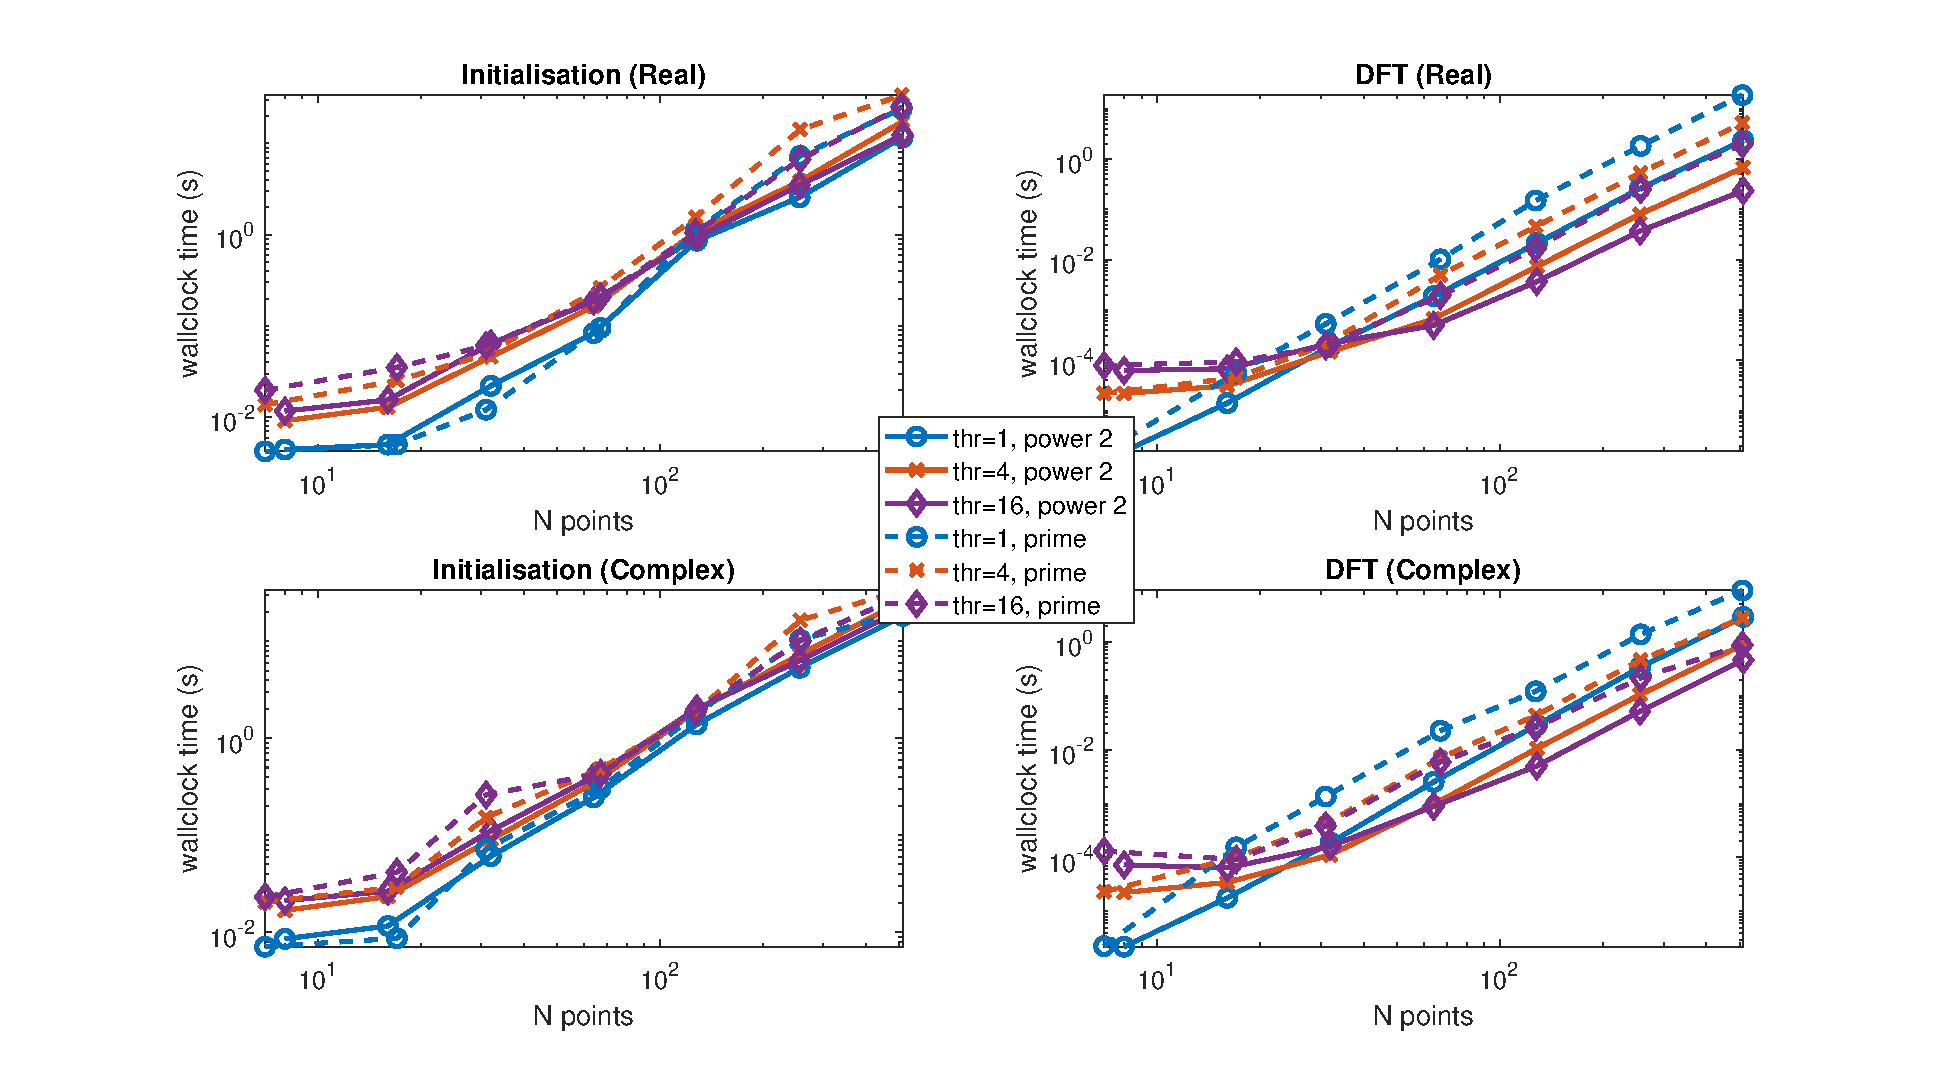
\includegraphics[width=0.9\linewidth]{../results/fftw_3d_thr.eps}
  \caption{Initialisation and DFT execution times of FFTW library applied to 3D signal as a function of the
    number of points, $N,$ and varying the number of threads, $thr.$ }
  \label{3DFFTW}
\end{figure}




\begin{table}
\begin{center}
%\being{small}
\begin{tabular}{|r||r|r||r|r||r|r||r|r|}
  \hline
 & \multicolumn{2}{|c||}{$k(N=31)$} & \multicolumn{2}{|c||}{$k(N=32)$} & \multicolumn{2}{|c||}{$k(N=509)$} & \multicolumn{2}{|c|}{$k(N=512)$} \\
$thr$ &  Real & Complex &  Real & Complex &  Real & Complex &  Real & Complex \\ \hline
  2 & 139  & -  &  825  & 420  & 1 &  6   & 8  & 10 \\
  4 & 114  & -  &  583  & 387  & 1 &  3   & 4  & 4  \\
  8 & 83   & -  &  -    & 353  & 1 &  2   & 2  & 2  \\
  12 & 149 & -  & 14367 & 1176 & 1 &  2   & 4  & 5  \\
  16 & 146 & -  &  -    & 1935 & 1 &  2   & 1  & 2  \\
  24 & 242 & -  &  -    &  -   & 0 &  1   & 3  & 3  \\ \hline
\end{tabular}
\caption{ For $N=31,$ 32, 509 and $N=512,$ the number of DFT calculations, $k,$ required for $thr$ threads to have a lower wallclock time than a single thread when performing  a single initialisation and $k$ DFT calculations are performed with the 3D interface to the FFTW library.  }\label{Tbl:FFTW3dk}
%\end{small}
\end{center}
\end{table}


\subsection{3D MKL Library}\label{Sec:3DMKL}

In Figure~\ref{3DMKL}, we compare the 3D benchmark runs for the MKL
library. As with the 2D runs, we observe that increasing the problem
size has little effect on the initialisation time when a single thread
is used: in this case there is also little difference in
initialisation time when switiching between $N$ being a power of 2 or
prime. When multiple threads are used, the initialisation times drops
significantly as the value of $N$ increases from 7 to 256. For $N=509$
and 512, the initialisation times are very similar to when a single
thread is used. In all cases, the initialisation time decreases when
moving from 4 to 16 threads. For further analysis, we provide the data
for $N=7,$ 8, 64, 67, 509 and 512 in Table~\ref{Tbl:MKL3d}. For $N=7,$
there is a factor of 6 difference in initialisation times when
comparing 1 and 16 threads. For a single thread and real input
signals, increasing $N$ from 7 to 509 increases the initialisation
time by 27\% and increasing $N$ from 8 to 512 increases the
initialisation time by 24\% whilst the overall problem size is
increased by over 5 orders of magnitude; for a single thread with
complex input signals, there are 18\% and 2\% increases in
initialisation times when $N$ increases from 7 to 509 and 8 to 512,
respectively. In comparison, for 16 threads and real input signals,
there are 80\% reductions in initialisation times when switching from
either $N=7$ to 509 or $N=8$ to 512; for complex input signals the
reduction is 77\%.

As expected, increasing $N$ increases the wallclock DFT time and the
time increases when switching from $N$ a power of 2 to the closer
prime number. In Figure~\ref{3DMKL}, we observe that when $N$ is
prime, the DFT decreases as the number of threads increases from 1 to
4 and then to 16 but there appears to be a bigger impact for larger
$N,$ and this is certainly the case for the values of $N$ provided in
Table~\ref{Tbl:MKL3d}. Additionally, multithreading has a lesser
impact when $N$ is a power of 2 than when $N$ is the nearest prime
number to a power of 2.

\begin{figure}[htb]
    \centering
    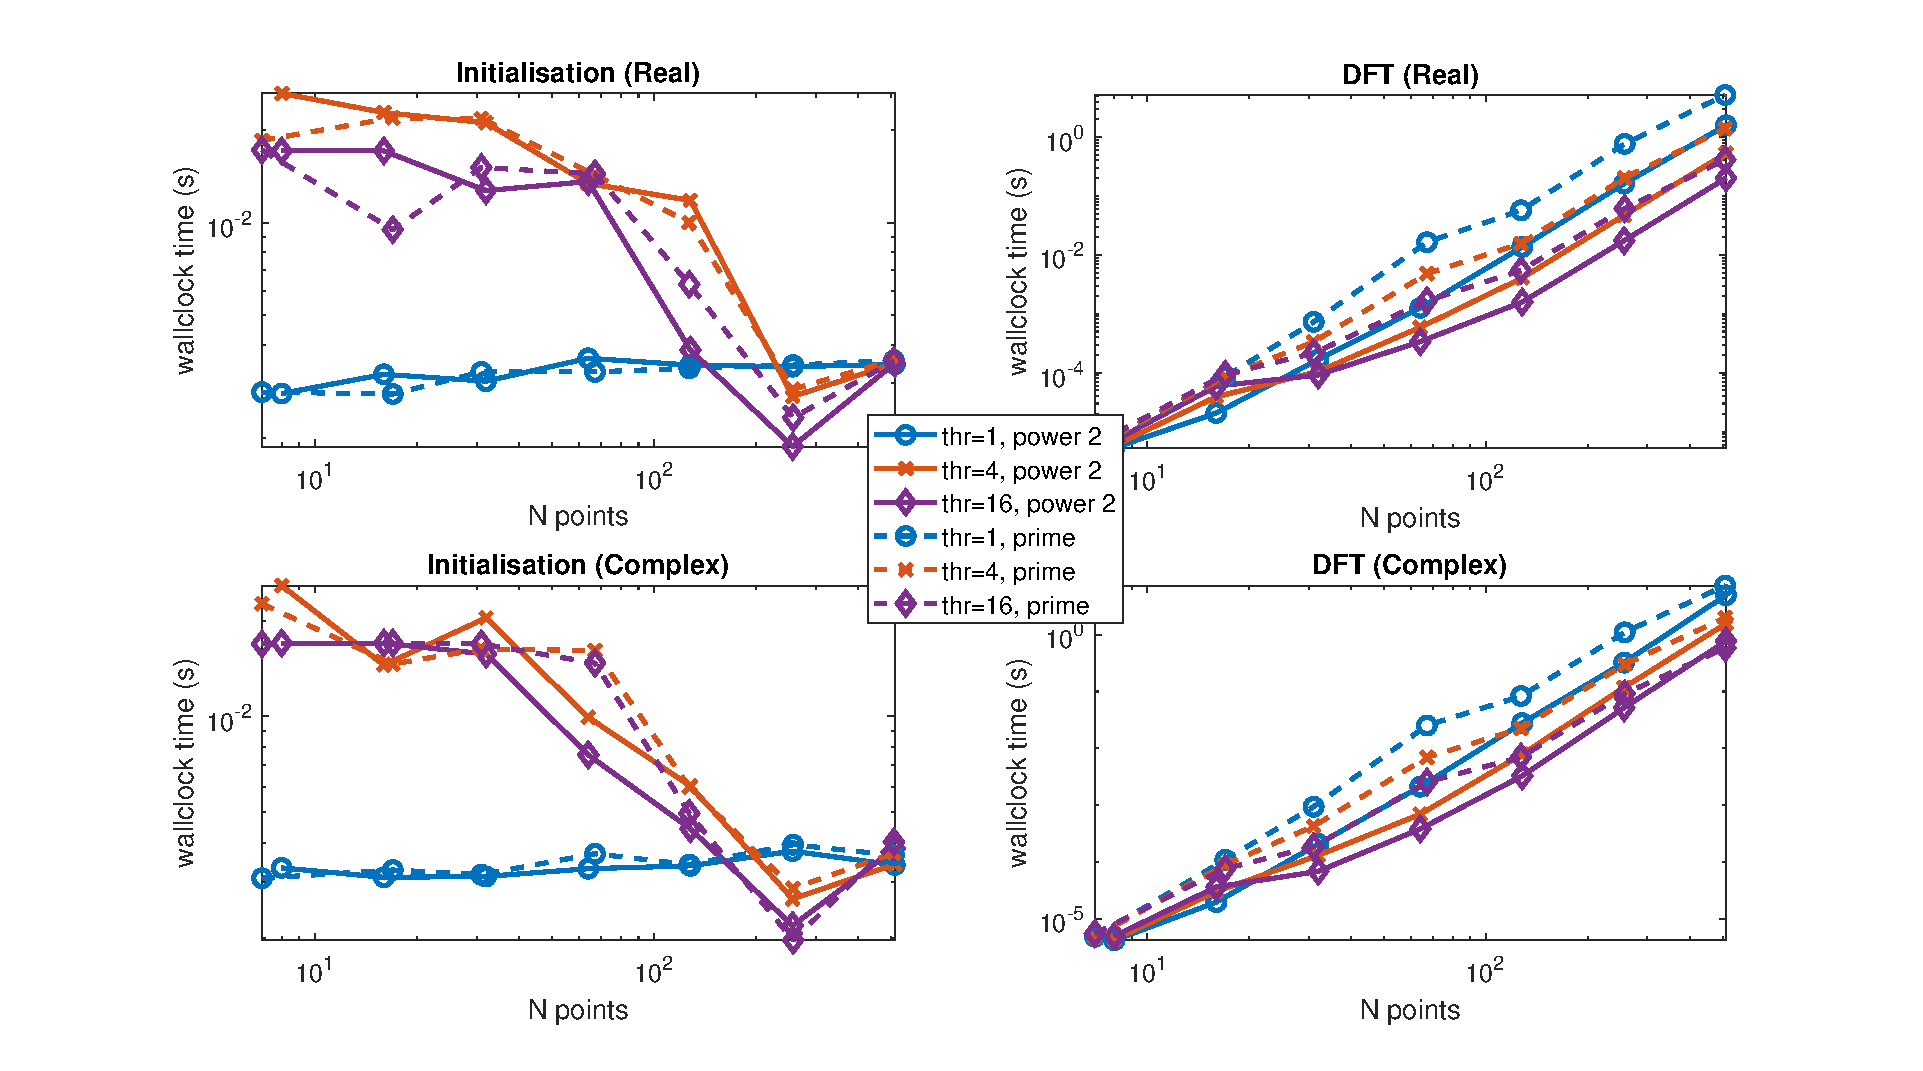
\includegraphics[width=0.9\linewidth]{../results/mkl_3d_thr.eps}
  \caption{Initialisation and DFT execution times of MKL library applied to 3D signal as a function of the
    number of points, $N,$ and varying the number of threads, $thr.$ }
  \label{3DMKL}
\end{figure}





As in Section~\ref{Sec:3DFFTW}, we have calculated the number of DFT
calculations, $k,$ (on average) that would be required for $thr$
threads to have a lower time than a single thread when performing a
single initialisation and $k$ DFT calculations for $N=31,$ 32, 509 and
$N=512:$ these values are provided in
Table~\ref{Tbl:MKL3dk}. Comparing the results for $N=31$ and $N=32,$
multithreading becomes more advantageous far sooner for the prime
value of $N$ and this is primarily because of multithreading having
more affect on the DFT wallclock time. For $N=509$ and $N=512,$ the
use of multiple threads is always advantageous in our benchmark
results.


\begin{table}
\begin{center}
%\being{small}
\begin{tabular}{|r||r|r||r|r||r|r||r|r|}
  \hline
 & \multicolumn{2}{|c||}{$k(N=31)$} & \multicolumn{2}{|c||}{$k(N=32)$} & \multicolumn{2}{|c||}{$k(N=509)$} & \multicolumn{2}{|c|}{$k(N=512)$} \\
$thr$ &  Real & Complex &  Real & Complex &  Real & Complex &  Real & Complex  \\ \hline
  2 & 32    & 25  & 446   & 119  & 1 &  1   & 1  &  1 \\
  4 & 48    & 26  & 292   & 225  & 1 &  1   & 1  &  1 \\
  8 & 44    & 26  & 242   & 152  & 1 &  1   & 0  &  1 \\
  12 & 25   & 24  & 193   & 98   & 1 &  1   & 1  &  1 \\
  16 & 24   & 19  & 129   & 91   & 0 &  1   & 1  &  1 \\
  24 & 26   & 17  & 250   & 101  & 1 &  0   & 1  &  1 \\ \hline
\end{tabular}
\caption{ For $N=31,$ 32, 509 and $N=512,$ the number of DFT calculations, $k,$ required for $thr$ threads to have a lower wallclock time than a single thread when performing  a single initialisation and $k$ DFT calculations are performed with the 3D interface to the MKL library.  }\label{Tbl:MKL3dk}
%\end{small}
\end{center}
\end{table}


\subsection{3D P3DFFT Library}\label{Sec:3DP3DFFT}
The P3DFFT library can only take real signals as input: we provide the
benchmark results in Figure~\ref{3DP3DFFT}. The initialisation times
for $N$ a power of 2 are always lower than when $N$ is a prime
number. With the exception of the 3 lowest values of $N$ is the two
different classes of $N,$ in general, multithreading reduces the
initialisation time as we move from 1 to 4 and then 4 to 16
threads. Increasing the problem size increases the initialisation
time. In Table~\ref{Tbl:P3DFFT3d}, we provide the benchmark data for
$N=7,$ 8, 31, 32, 509 and 512. For the largest values of $N$
considered, the effect of multithreading on the wallclock
initialisation time is greater when $N$ is a power 2 than when $N$ is
prime.

Considering the DFT results in Figure~\ref{3DP3DFFT}, when $N$ is a
power of 2 and less than or equal to 64, increasing the number of
threads is also increasing the DFT time; for the larger values of $N$
increasing the number of threads decreases the wallclock DFT time but
there appears to be little difference between 4 and 16 threads,
however, Table~\ref{Tbl:P3DFFT3d} reveals that the DFT time for four
threads is 31\% higher than that of sixteen threads. For prime values
of $N,$ when $N$ is smaller than 31 we observe that increasing the
number of threads increases the DFT time but for larger values of $N$
we get a decrease in DFT time. For $n=509,$ the DFT wallclock time
ratio relative to a single thread is 0.34 for 4 threads, 0.17 for 16
threads and 0.16 for 24 threads. Multithreading has a bigger effect on
DFT time when $N$ is prime compared on $N$ being a power of 2.



\begin{figure}[htb]
    \centering
    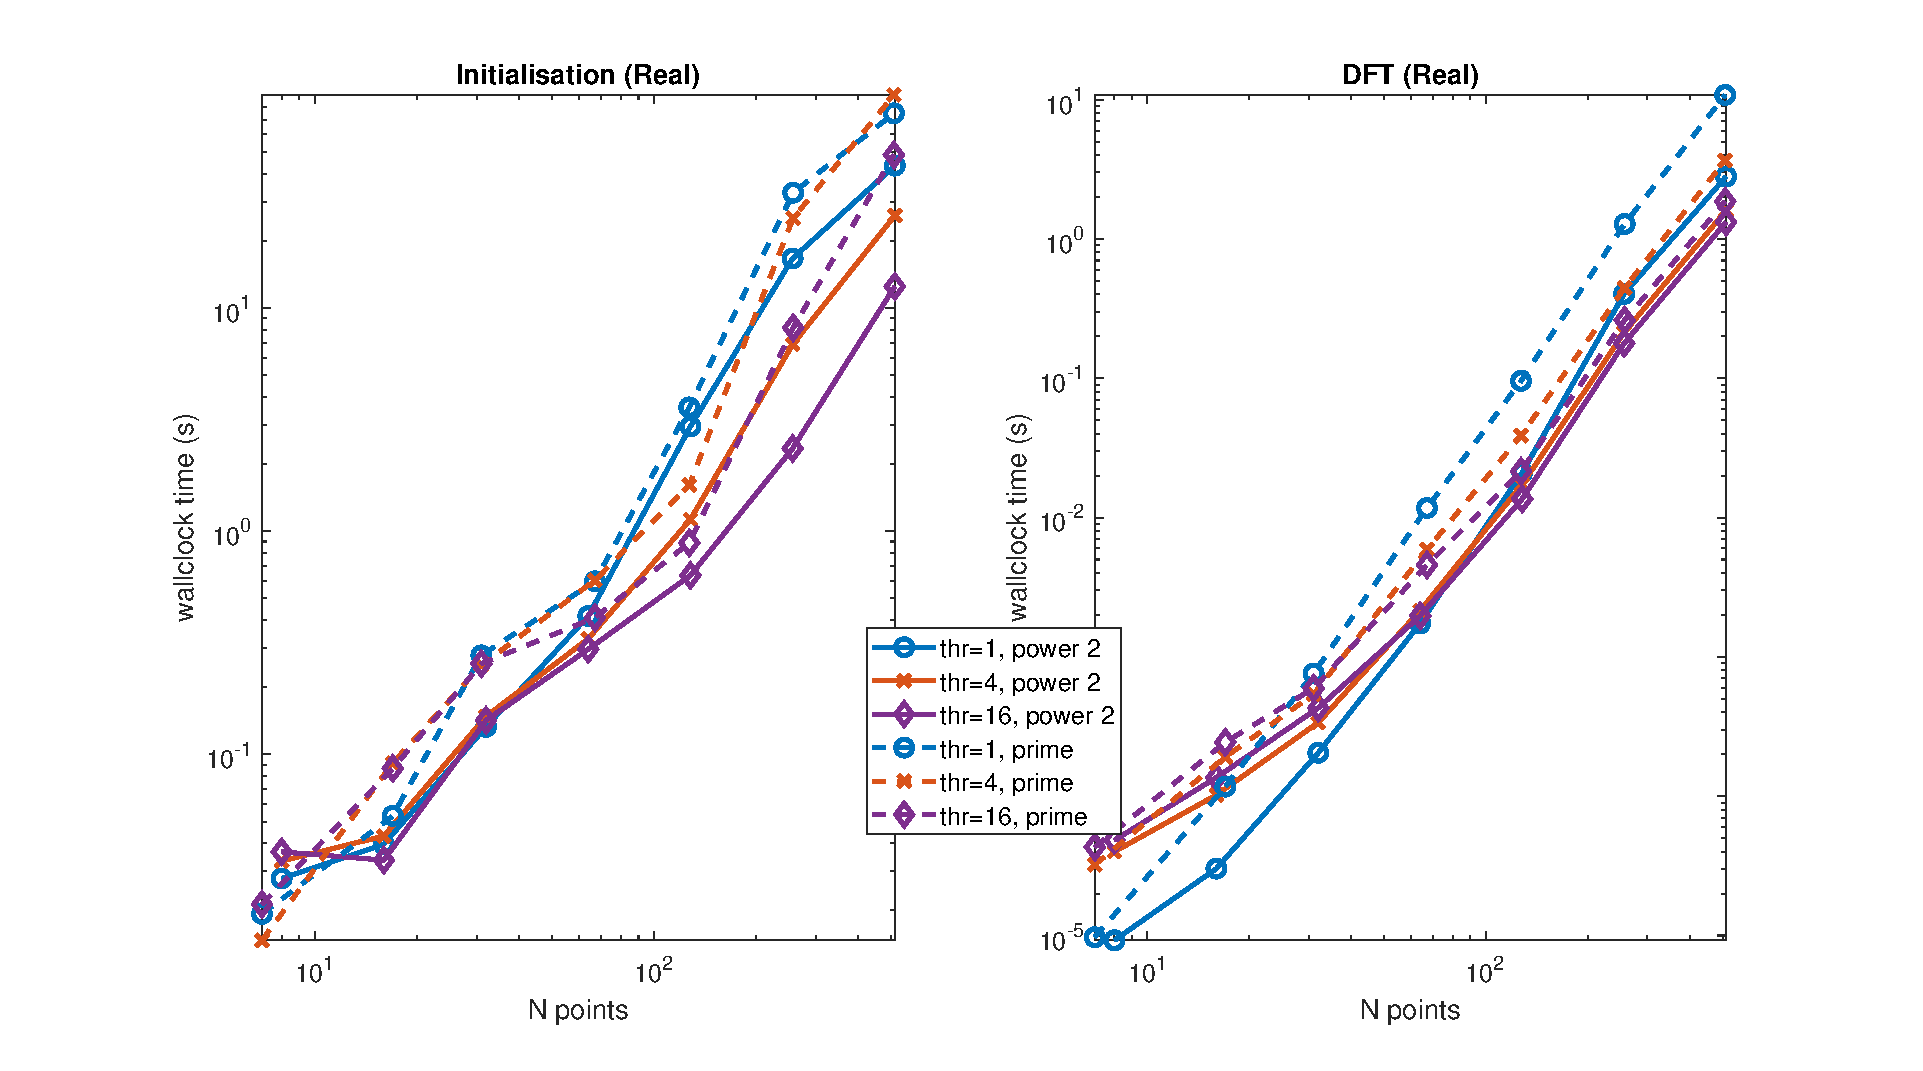
\includegraphics[width=0.9\linewidth]{../results/p3dfft_3d_thr.eps}
  \caption{Initialisation and DFT execution times of P3DFFT library applied to 3D signal as a function of the
    number of points, $N,$ and varying the number of threads, $thr.$ }
  \label{3DP3DFFT}
\end{figure}







\subsection{Comparison of libraries for 3D benchmarks}\label{Sec:3DComp}

We compare the initialisation and DFT wallclock times for FFTW, MKL
and P3DFFT in Figures~\ref{fig:3DComp2} ($N$ a power of 2) and
\ref{fig:3DFFTWMKLPrime} ($N$ prime). Considering the initialisation
times, MKL is the fastest and P3DFFT is, in general, the slowest in
the real input signal cases: for large values of $N$ there is between
3 and 4 orders of magnitude in difference.

Considering the DFT times, the different packages have similar
times. Combining all of these comparisons together, we conclude that
the MKL library is, in general, outperforming both the FFTW and P3DFFT
libraries.


\begin{figure}[htbp]
    \centering
    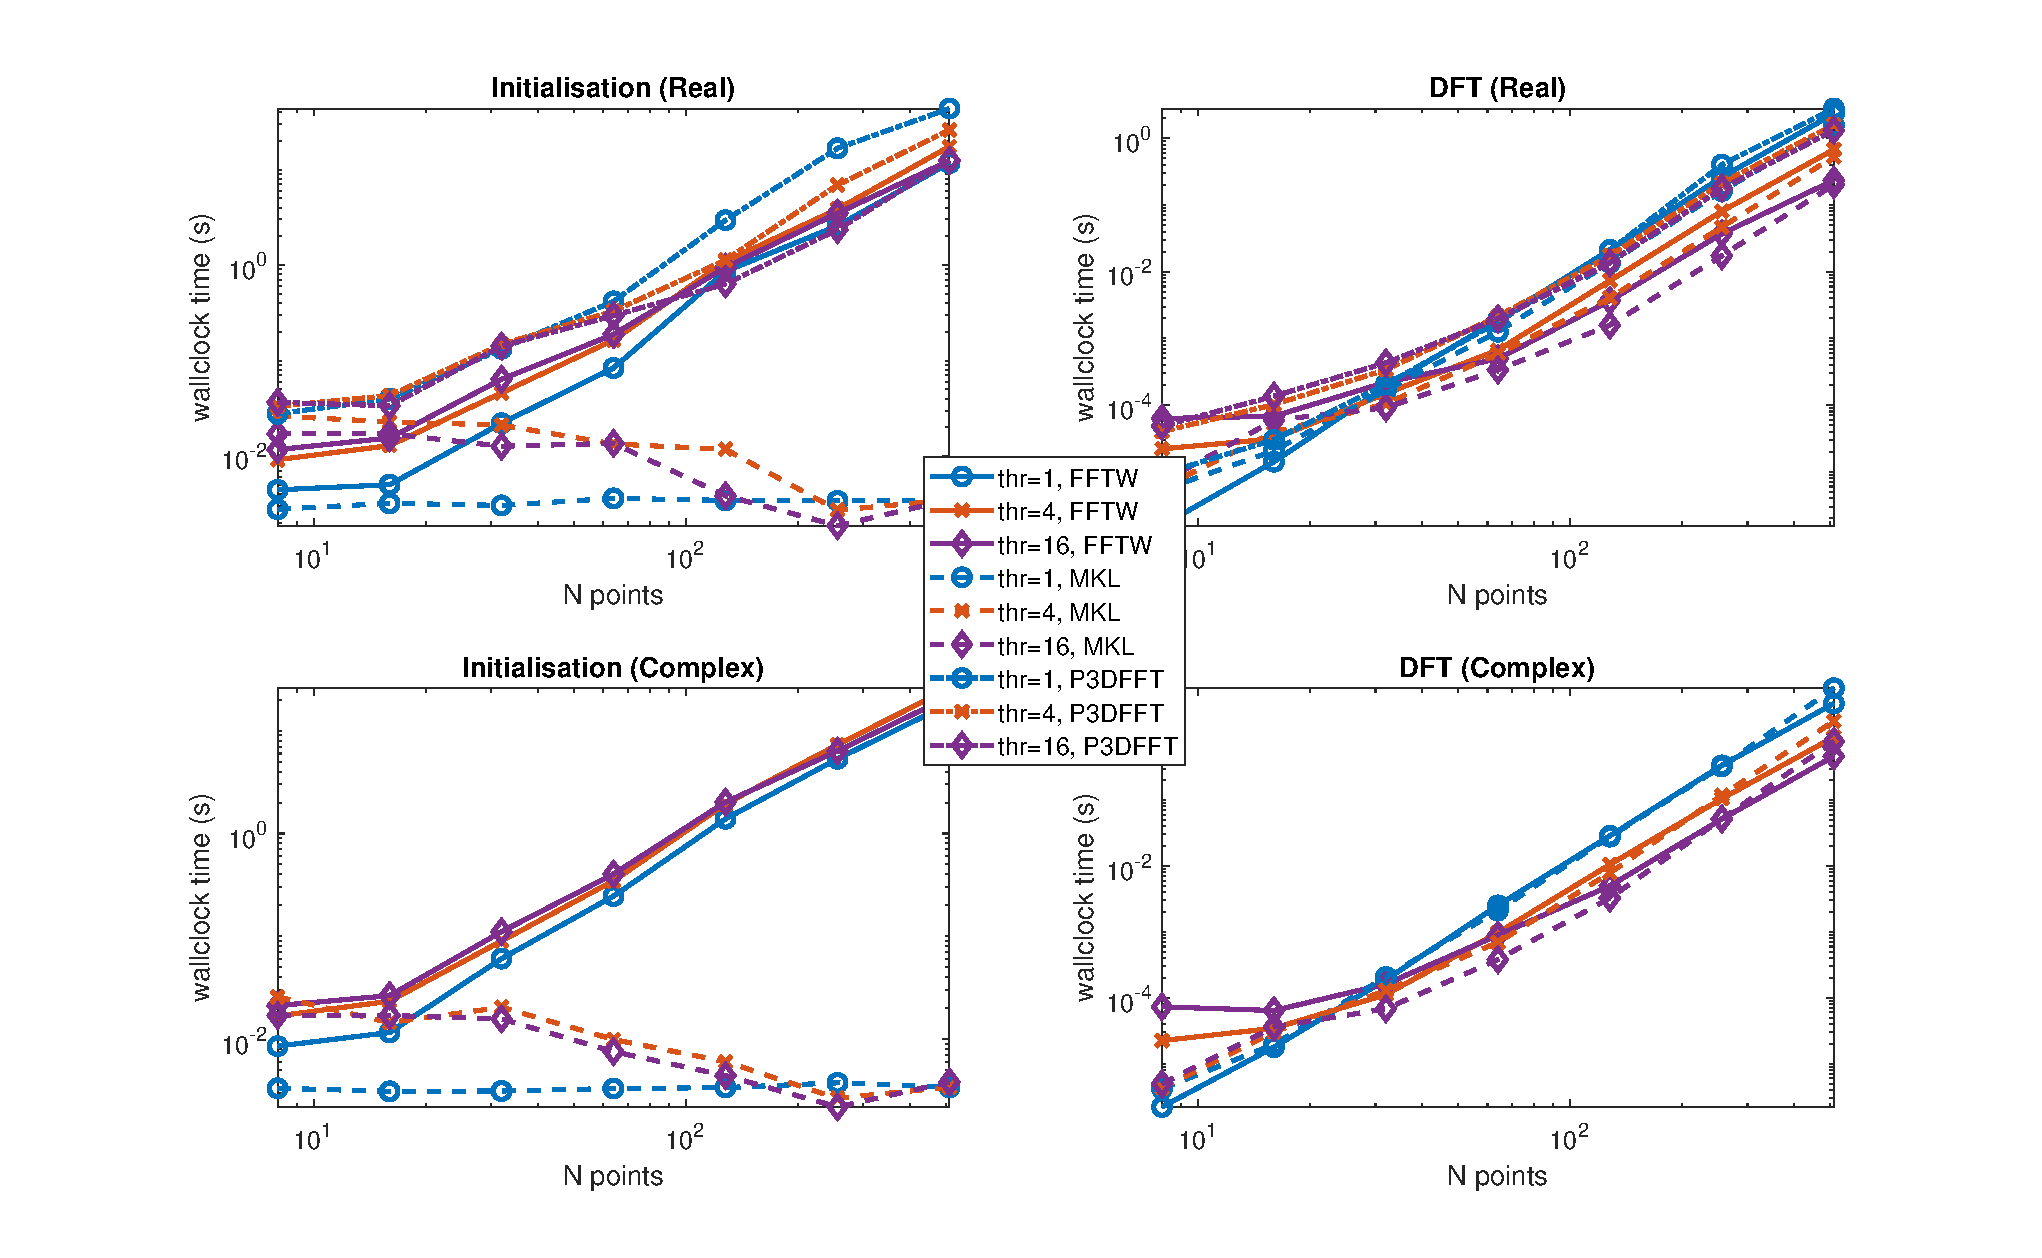
\includegraphics[width=0.9\linewidth]{../results/fftw_mkl_p3dfft_2_3d_thr.eps}
  \caption{Initialisation and DFT execution times of FFTW, MKL and P3DFFT libraries applied to 3D signal as a function of the number of points, $N,$ and varying the number of threads, $thr.$ $N$ is a power of 2. }
  \label{fig:3DComp2}
\end{figure}


\begin{figure}[htb]
    \centering
    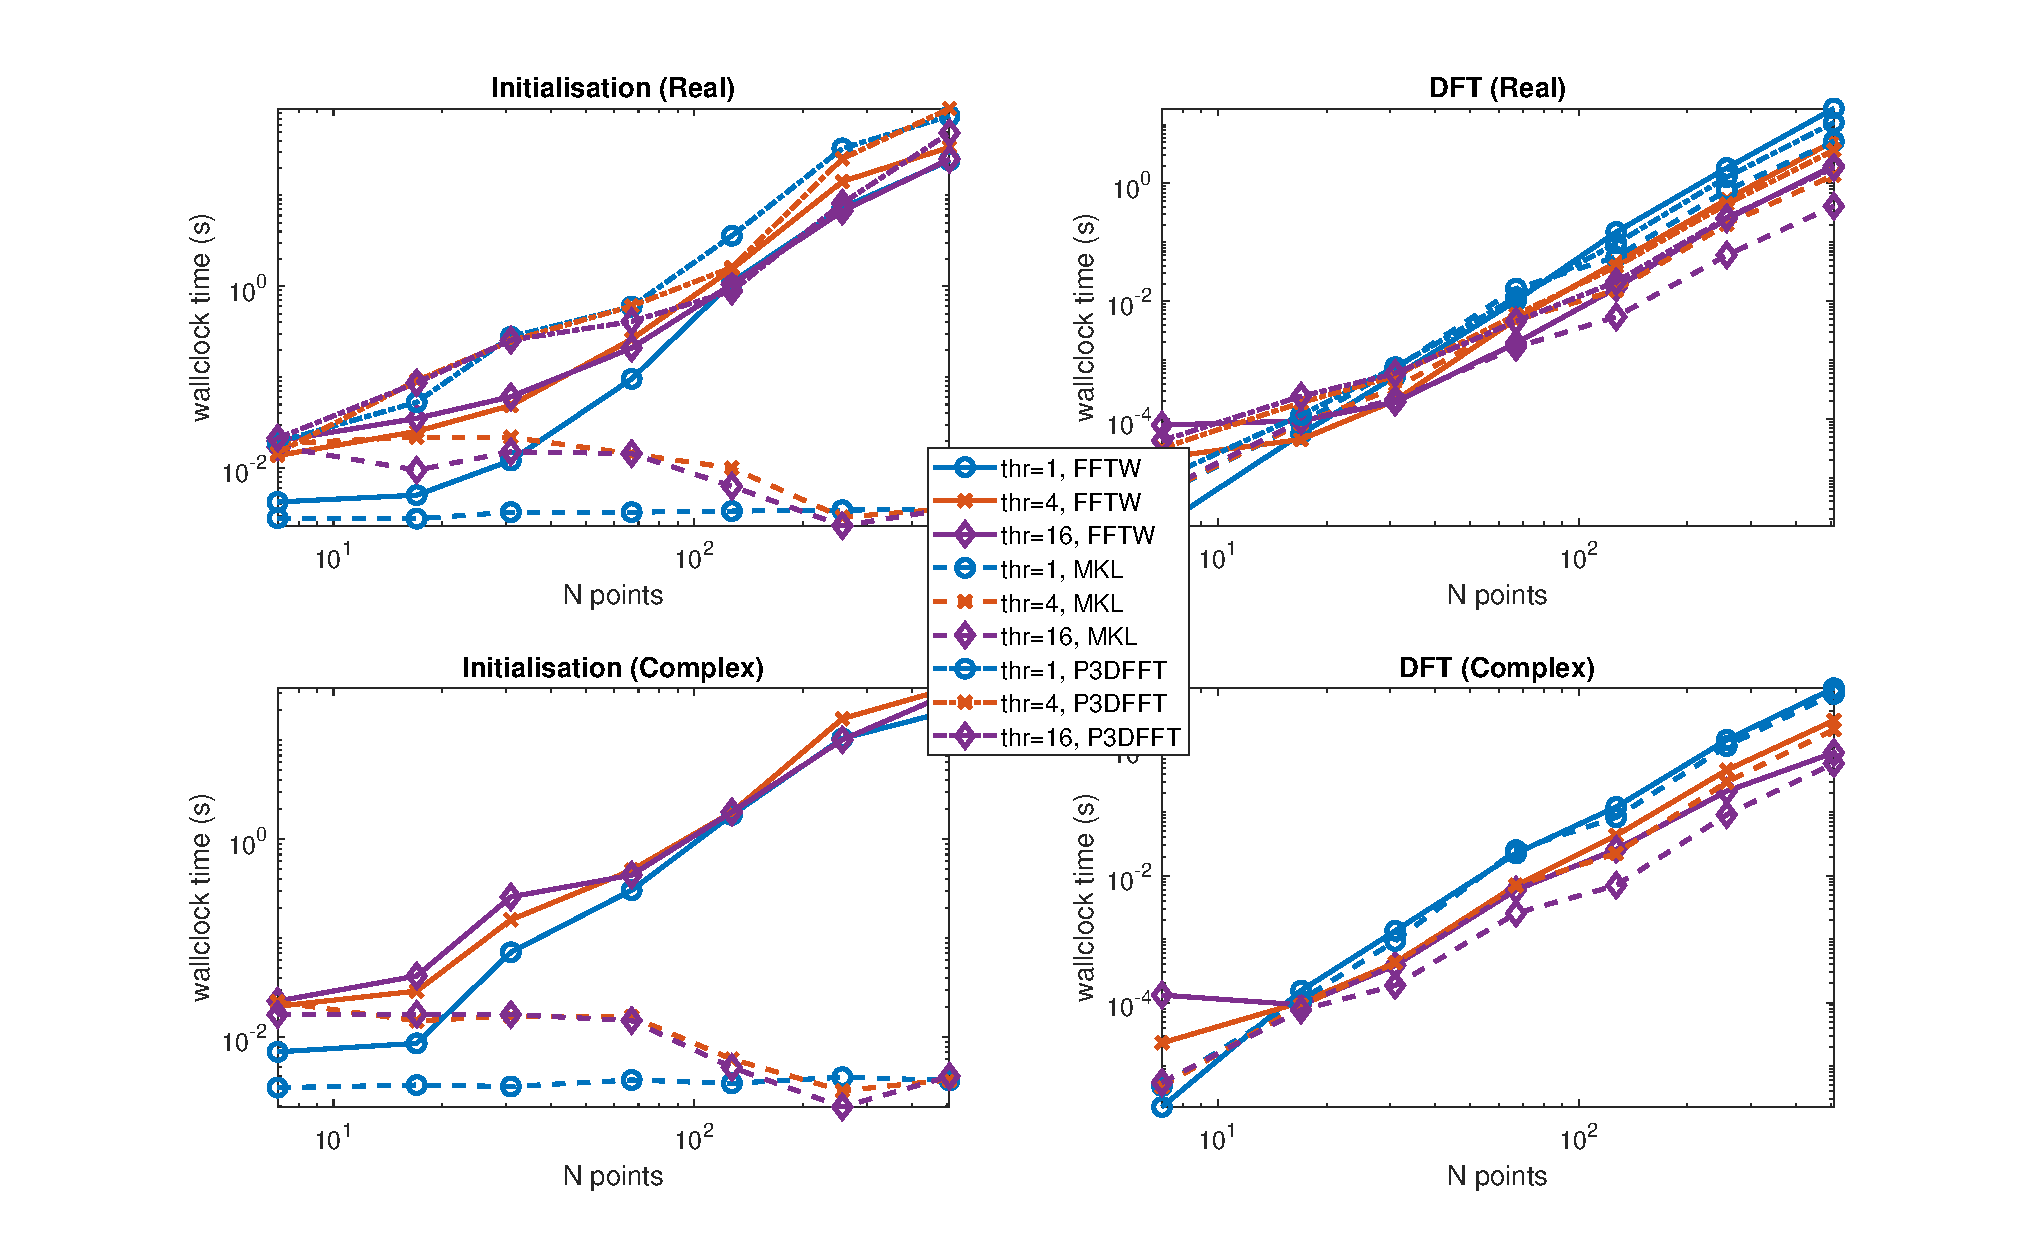
\includegraphics[width=0.9\linewidth]{../results/fftw_mkl_p3dfft_prime_3d_thr.eps}
  \caption{Initialisation and DFT execution times of FFTW, MKL and P3DFFT libraries applied to 3D signal as a function of the number of points, $N,$ and varying the number of threads, $thr.$ $N$ is a prime number.}
  \label{fig:3DFFTWMKLPrime}
\end{figure}



\clearpage

\section{Effect of domain size and distributed parallelisation for 1D benchmarks}\label{Sec:1DDistr}
In this section, we discuss the benchmark results for distributed
libraries that apply the fast Fourier transform to 1D arrays.  The
P3DFFT library cannot be used on 1D problems and, hence, is
excluded. These benchmarks were performed with the MPI-OpenMP versions
of FFTW and MKL. 

As in Section~\ref{Sec:1DMulti}, we set $n_2=4,$ $n_q=4$ and $n_1=N,$ were $N$ is
defined as follows.  For one set of tests, we let $N=2^k$ for
$k=8,\ldots,20.$ For the other set of tests, $N$ is defined to be the
closest prime number to $2^k,$ $k=8,\ldots,20:$ if two primes are
equidistant, we choose the larger one.

\subsection{1D Distributed FFTW Library}\label{Sec:1DDistFFTW}

The distributed version of the FFTW library only
provides a 1D interface for complex input signals. As with the
multithreaded benchmark results, we are restricted to values of $N$
that are at most $2^{14}.$ We also found that the library had a bug
when 12 or 24 MPI processes where requested and would crash.

In Figure~\ref{1DDistFFTW}, we compare our benchmark results for 1, 4
and 16 MPI processes, $P,$ with a single thread per process. When
$P=16,$ we observe a bump in the initialisation times at $N=1024:$
further analysis of the benchmark data revealed that this bump was
replicated across all of the benchmark runs. For the larger values of
$N,$ increasing the number of processes decreases the initialisation
times when $N$ is a power of 2 but there is little change when $N$ is
prime. Looking at DFT times, when $N$ is a power of 2, we observe an
increase in wallclock time as we increase the number of processes in
all but the larger values of $N$ but the restriction in size of $N$
means that we are barely seeing any advantage in using multiple
processes. When $N$ is prime, increasing the number of processes
results in a small increase in DFT wallclock time.


\begin{figure}[htb]
    \centering
    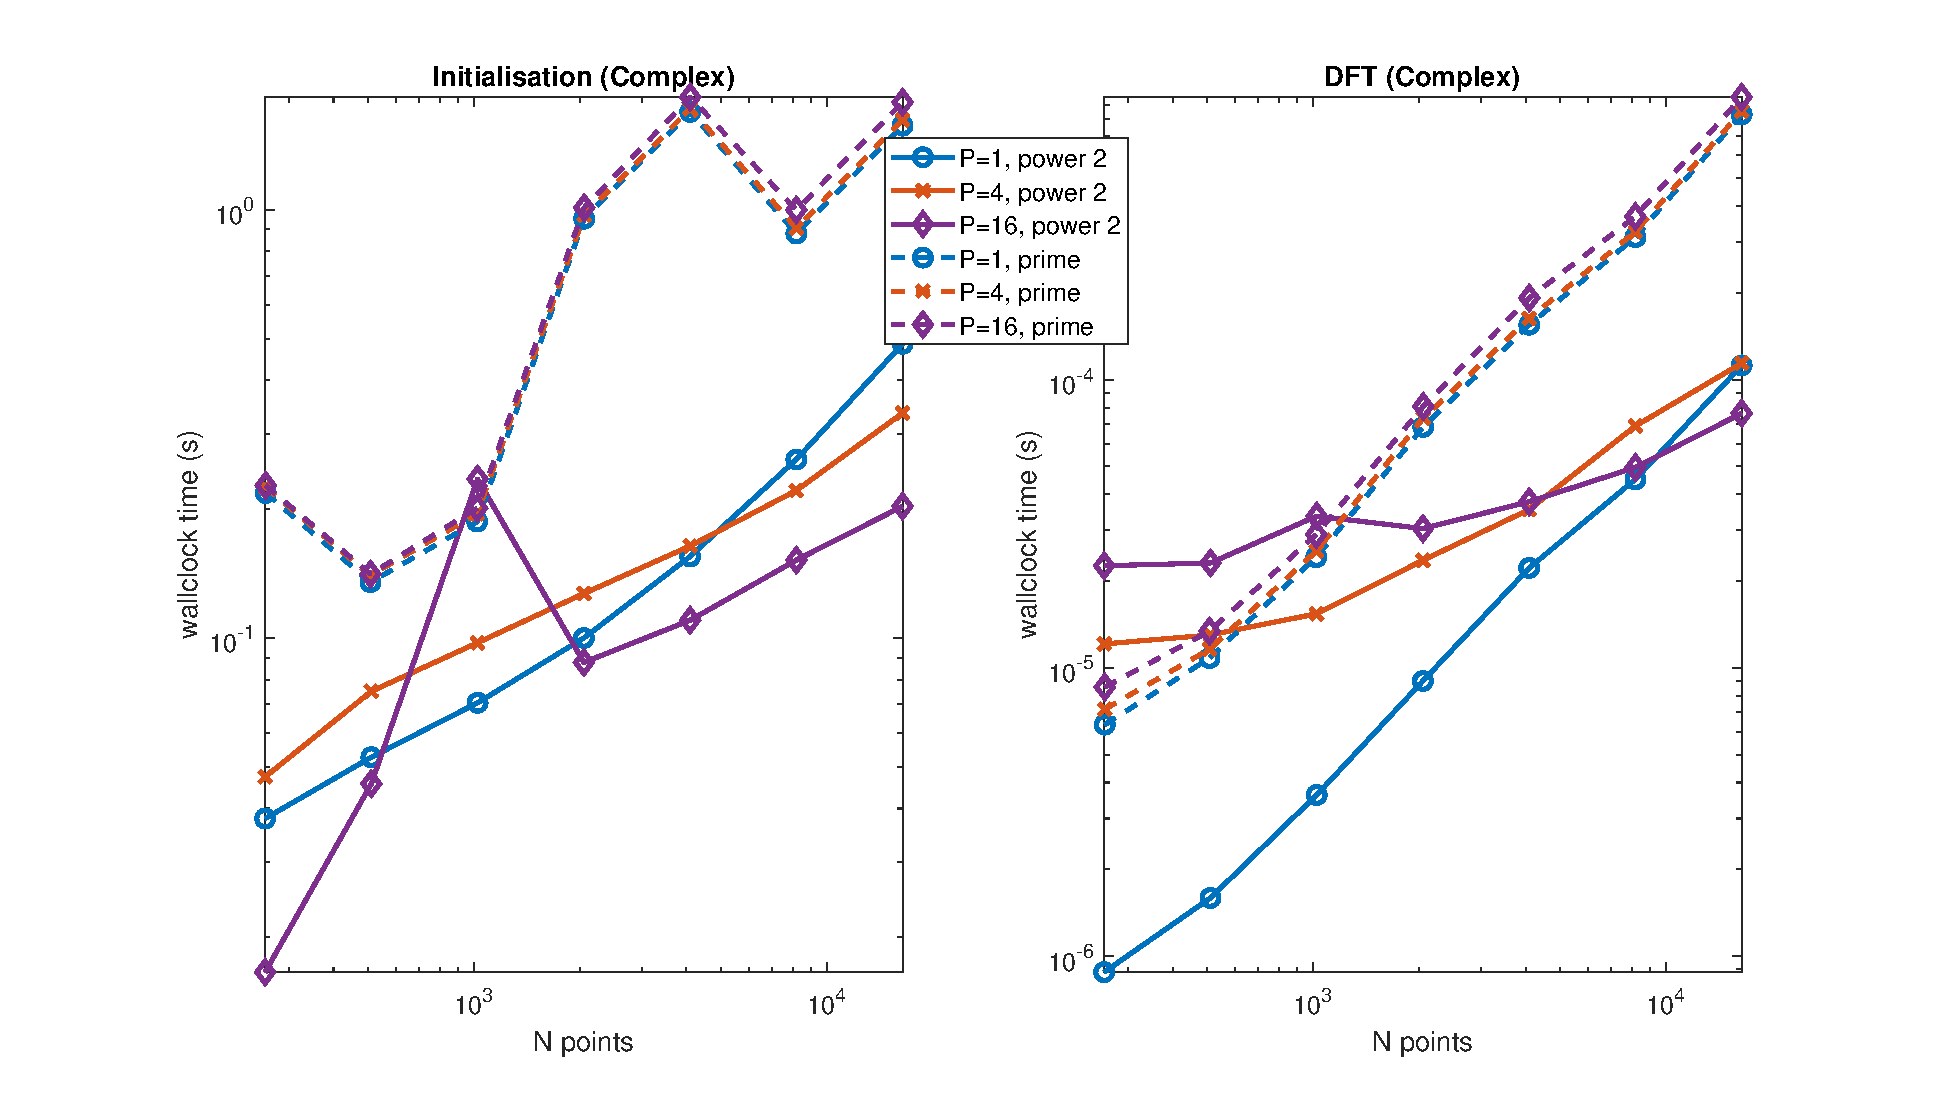
\includegraphics[width=0.9\linewidth]{../results/fftw_1d_mpi.eps}
  \caption{Initialisation and DFT execution times of distributed FFTW library applied to 1D signal as a function of the
    number of points, $N,$ and varying the number of MPI processes, $P,$ with one thread per process.}
  \label{1DDistFFTW}
\end{figure}

In Figure~\ref{1DDistFFTW16}, we compare our benchmark test results
when $P\times thr=16$ and $P=1,$ 4 and 16, and observe that it was, in
general, better to use a single thread with 16 MPI processes in the
benchmarks compared. For $N=16381,$ we provide all of the data and
ratios relative to using $P=1$ and $thr=1$ in
Table~\ref{Tbl:FFT1d16381} (Appendix~\ref{App:1Ddist}) and find that the combination of one MPI
process with four threads was optimal. In Table~\ref{Tbl:FFT1d16384}
we provide the data for $N=16384$ and discover that 16 MPI processes
and a single thread per MPI process was optimal. However, we cannot
take $N$ large enough to find a general trend.

\begin{figure}[htb]
    \centering
    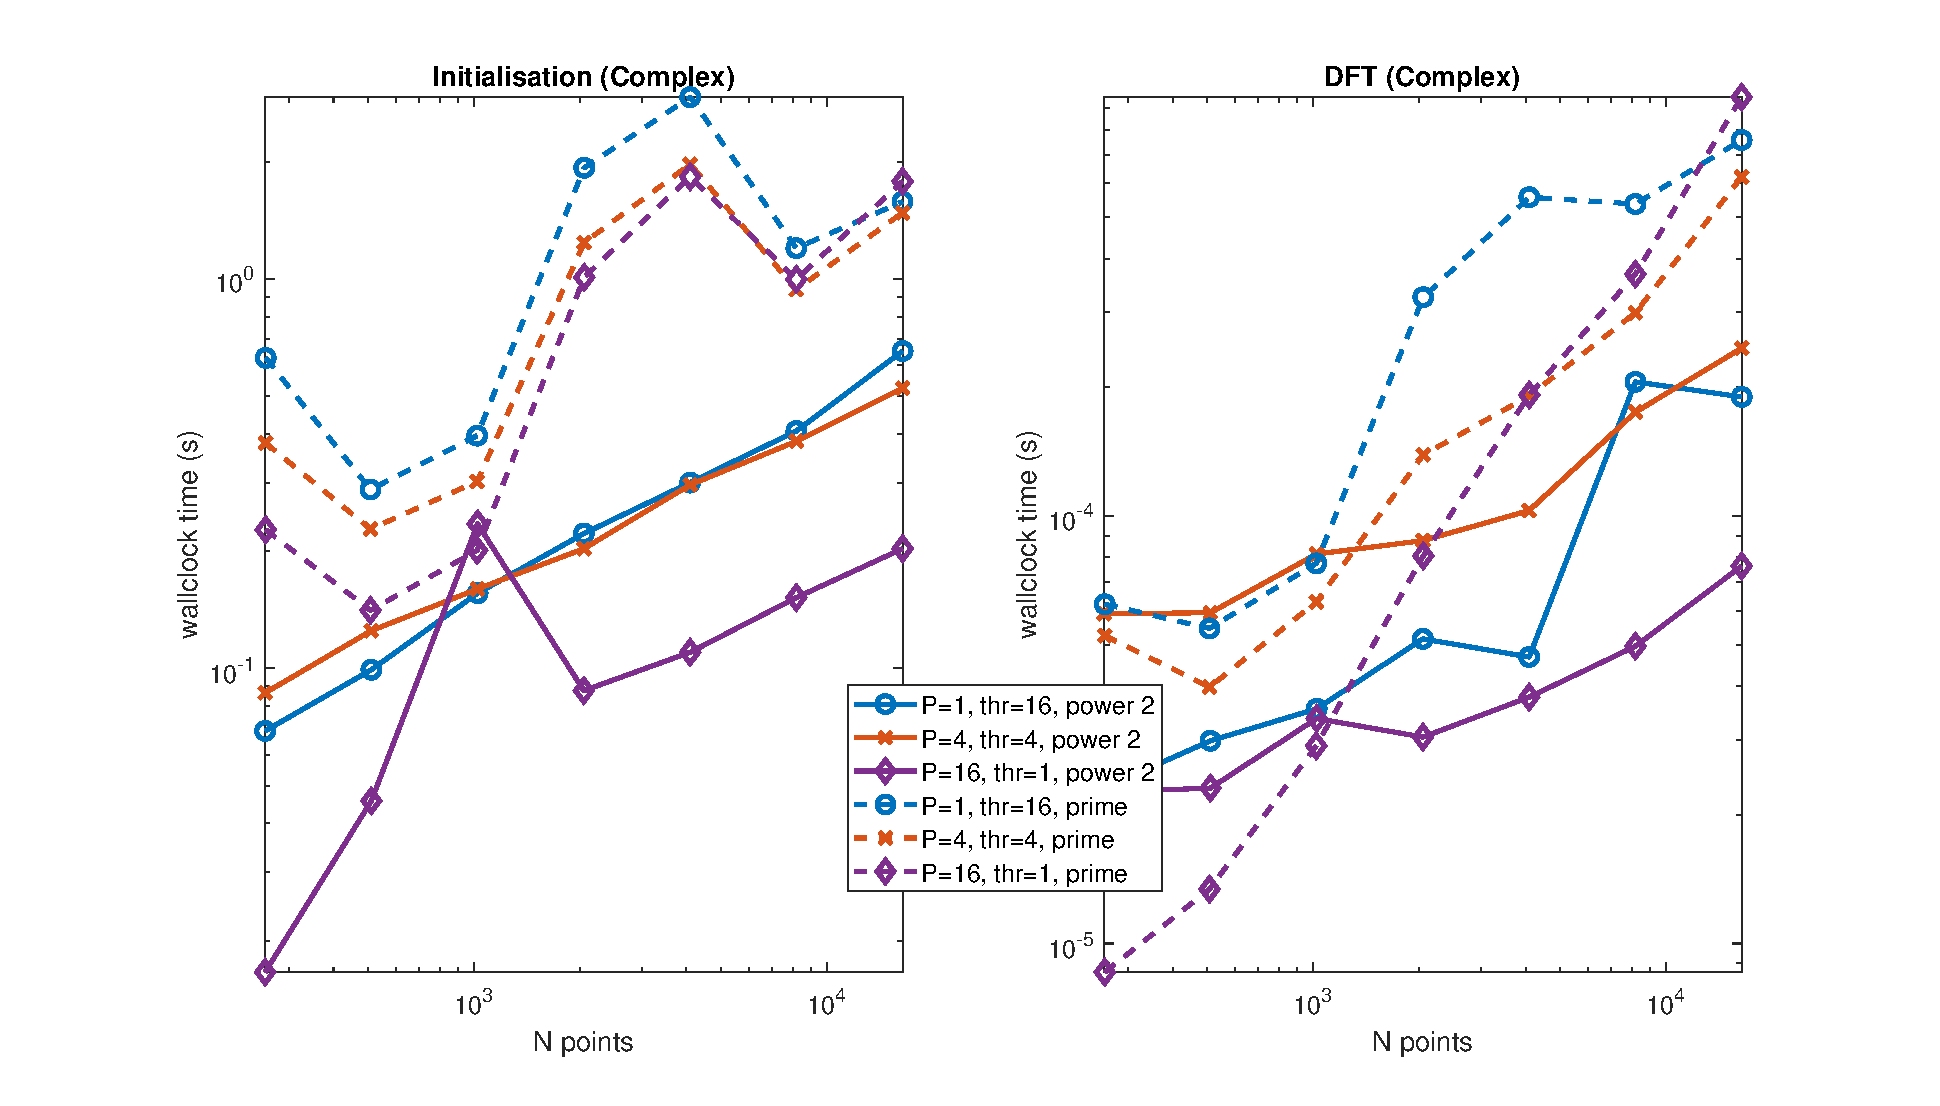
\includegraphics[width=0.9\linewidth]{../results/fftw_1d_mpi_thr.eps}
  \caption{Initialisation and DFT execution times of distributed FFTW library applied to 1D signal as a function of the
    number of points, $N,$ and varying the number of MPI processes, $P,$ and threads, $thr,$ whilst maintaining $P\times thr=16.$}
  \label{1DDistFFTW16}
\end{figure}









\subsection{1D Distributed MKL Library}\label{Sec:1DDistMKL}
In contrast to the distributed FFTW library, the distributed MKL
library has 1D interfaces for both real and complex input
signals. However, the interface does not allow prime values of $N.$


Using one thread per MPI process, we compare our benchmark results for
$P=1,$ 4 and 16 in Figure~\ref{1DDistMKL}. For $N<10^4,$ the
initialisation times remain almost constant as the size of $N$
increases with $P=4$ having an initialisation time that is roughly 15
times larger than that of a single process and $P=16$ being roughly 30
times larger that the single process, with the real and complex
benchmarks having very similar values. In Table~\ref{Tbl:MKL1d16384},
we provide the data for $N=16384$ and ratios with respect to $P=1$ and
$thr=1.$ We start by observing that, for a single thread per MPI
process, increasing the number of processes has a larger effect on
initialisation time when the input signal is real instead of being
complex and, hence, the initialisation times are slightly lower for
the complex case when a large number of processes are used. For
$N>10^4,$ the difference in initialisation times for different numbers
of MPI processes appears to narrow in Figure~\ref{1DDistMKL}: the data
for $N=1048576$ is provided for in Table~\ref{Tbl:MKL1d1048576} and
the values of iratio are much lower than those in
Table~\ref{Tbl:MKL1d16384} but increasing the number of processes
still, in general, increases the initialisation times.

Comparing the DFT wallclock execution times in Figure~\ref{1DDistMKL},
for $N\le 10^5$ (real case) or $N\le 2\times 10^4$ (complex case), a
single process gives the optimal wallclock execution time. For larger
vales of $N,$ we observe that increasing the number of processes from
1 to 4 and then to 16 decreases the DFT time. In
Table~\ref{Tbl:MKL1d16384}, we observe that, in the complex case with
$N=16384,$ there is an improvement in DFT time when two or four
processes are used. When $N=1048576$ (Table~\ref{Tbl:MKL1d1048576}),
increasing the number of processes (with a single thread per process)
produces a monotonic decrease in DFT time.

We compare our results for the case $P\times thr=16$ with $P=1,$ 4 and
16 in Figure~\ref{1DDistMKL16}. For all values of $N$ considrered,
increasing the value of $P$ increases the initialisation time: using
Table~\ref{Tbl:MKL1d16384}, when $N=16384$ with real input signal,
switching from $P=1$ and $thr=16$ to $P=16$ and $thr=1$ increases the
initialisation time by a factor of 4.9; for $N=1048576$
(Table~~\ref{Tbl:MKL1d1048576}), the increase is a factor of 2.5. In
terms of DFT times, when $N$ is small, Figure~\ref{1DDistMKL16}
reveals that a single MPI process with 16 threads is better than the
other combinations considered. For the larger values of $N,$ 16 MPI
processes with a single thread per process is the optimal choice in
Figure~\ref{1DDistMKL16}. 



\begin{figure}[htb]
    \centering
    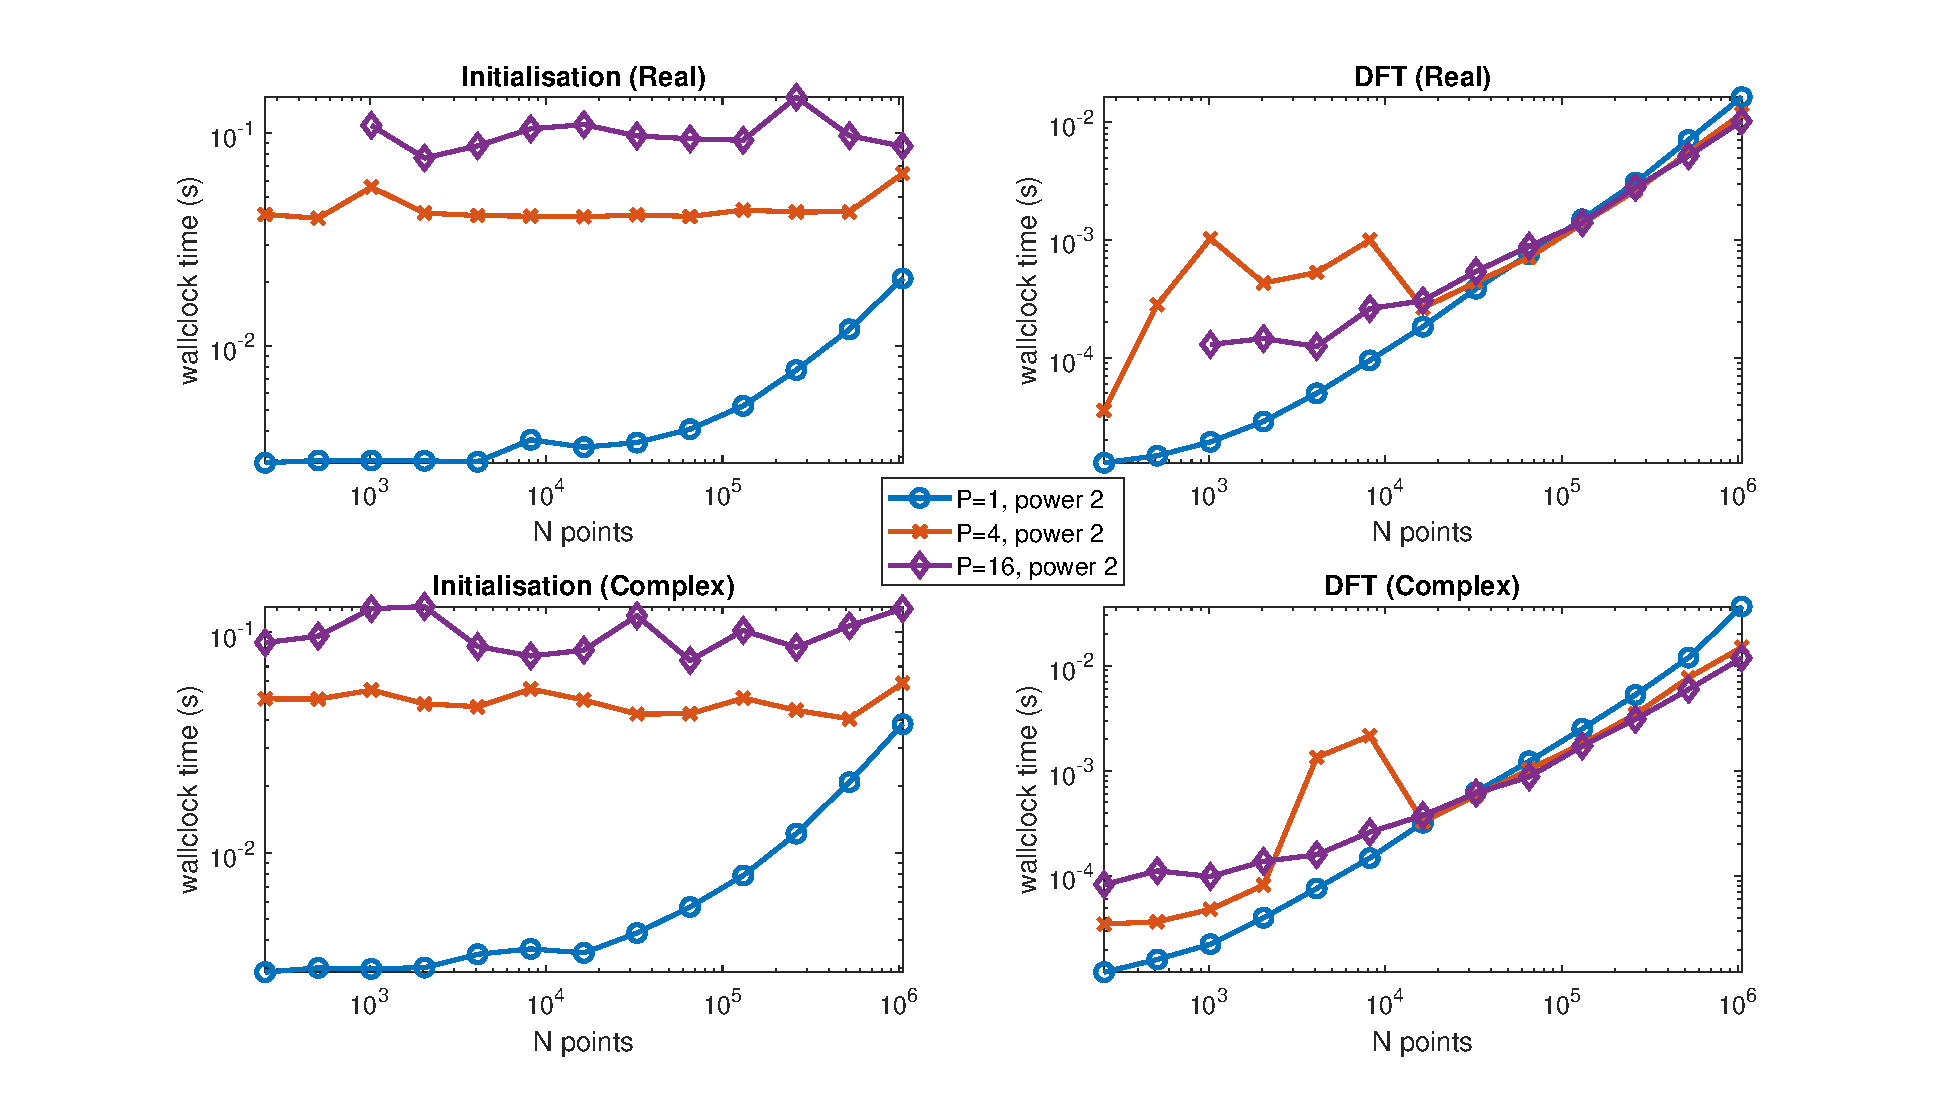
\includegraphics[width=0.9\linewidth]{../results/mkl_1d_mpi.eps}
  \caption{Initialisation and DFT execution times of distributed MKL library applied to 1D signal as a function of the
    number of points, $N,$ and varying the number of MPI processes, $P,$ with one thread per process.}
  \label{1DDistMKL}
\end{figure}

\begin{figure}[htb]
    \centering
    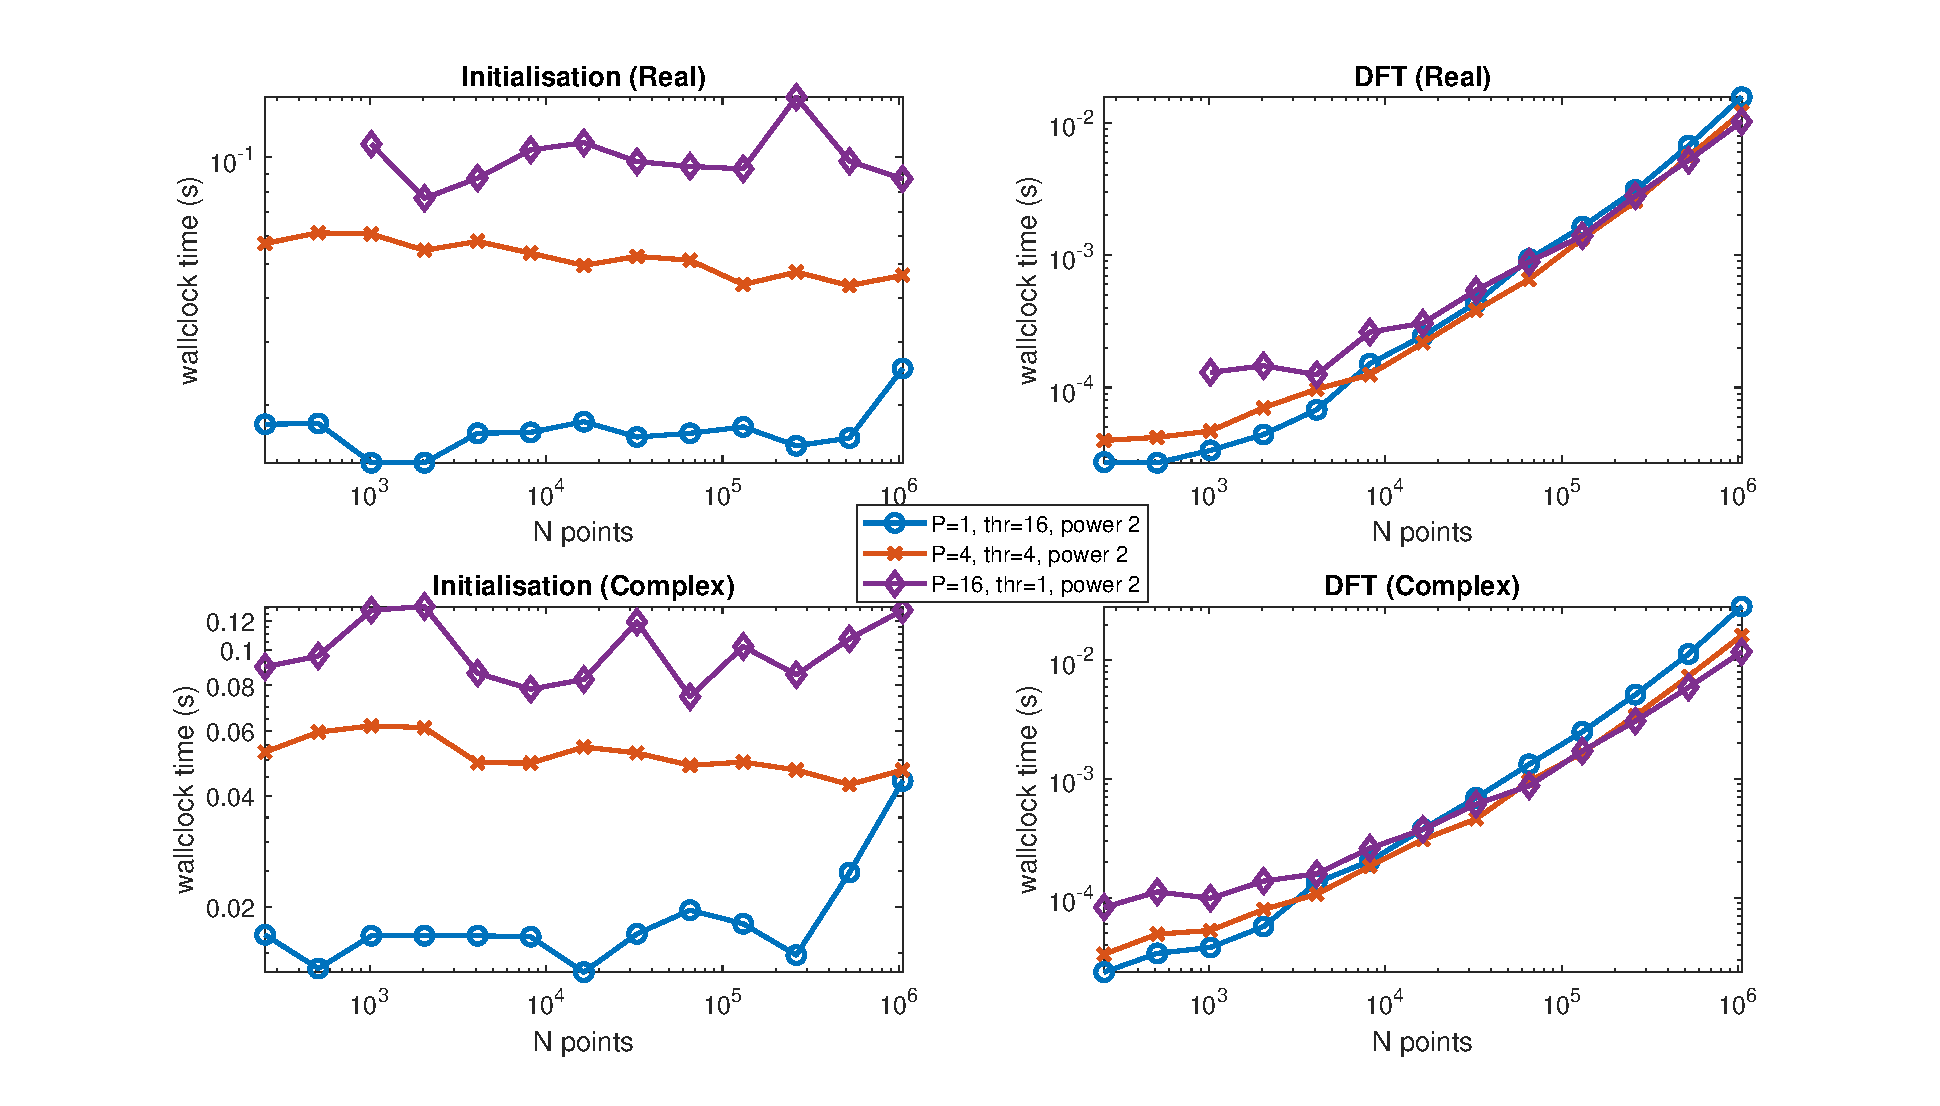
\includegraphics[width=0.9\linewidth]{../results/mkl_1d_mpi_thr.eps}
  \caption{Initialisation and DFT execution times of distributed MKL library applied to 1D signal as a function of the
    number of points, $N,$ and varying the number of MPI processes, $P,$ and threads, $thr,$ whilst maintaining $P\times thr=16.$}
  \label{1DDistMKL16}
\end{figure}






\subsection{Comparison of distributed libraries for 1D benchmark}\label{Sec:1DDistComp}

It is not possible to compare the distributed 1D interfaces when $N$
is prime because the MKL interface cannot handle such values of $N$
although we note that the 2D interface could be used to do such a
comparison. The FFTW library only provides a 1D interface for complex
signals but, in the following, we compare both FFTW and MKL with real
and complex inputs by transforming the real input values into complex
values and then feeding them into the FFTW interface,
Figure~\ref{1DDistFFTWMKL2}. On ARCHER, the MKL library allows for
much larger values of $N$ than FFTW. Additionally, the initialisation
times are better for the MKL library. For small values of $N,$ FFTW
has lower DFT times but, since the DFT times are several orders of
magnitude smaller than the initialisation times, the user will only
see an overall gain (initialisation time plus $l$ DFT calculations) to
using FFTW if $l$ is large. For the complex case and $N=16384,$ we
provide the minimal value of $l$ such that the overall initialisation
time plus time to perform $l$ DFT calculations is lower for FFTW than
MKL in Table~\ref{Tbl:1Dl}. We conclude, that when the 1D MKL
interface can be used, it is generally best to use the MKL library.

\begin{figure}[htb]
    \centering
    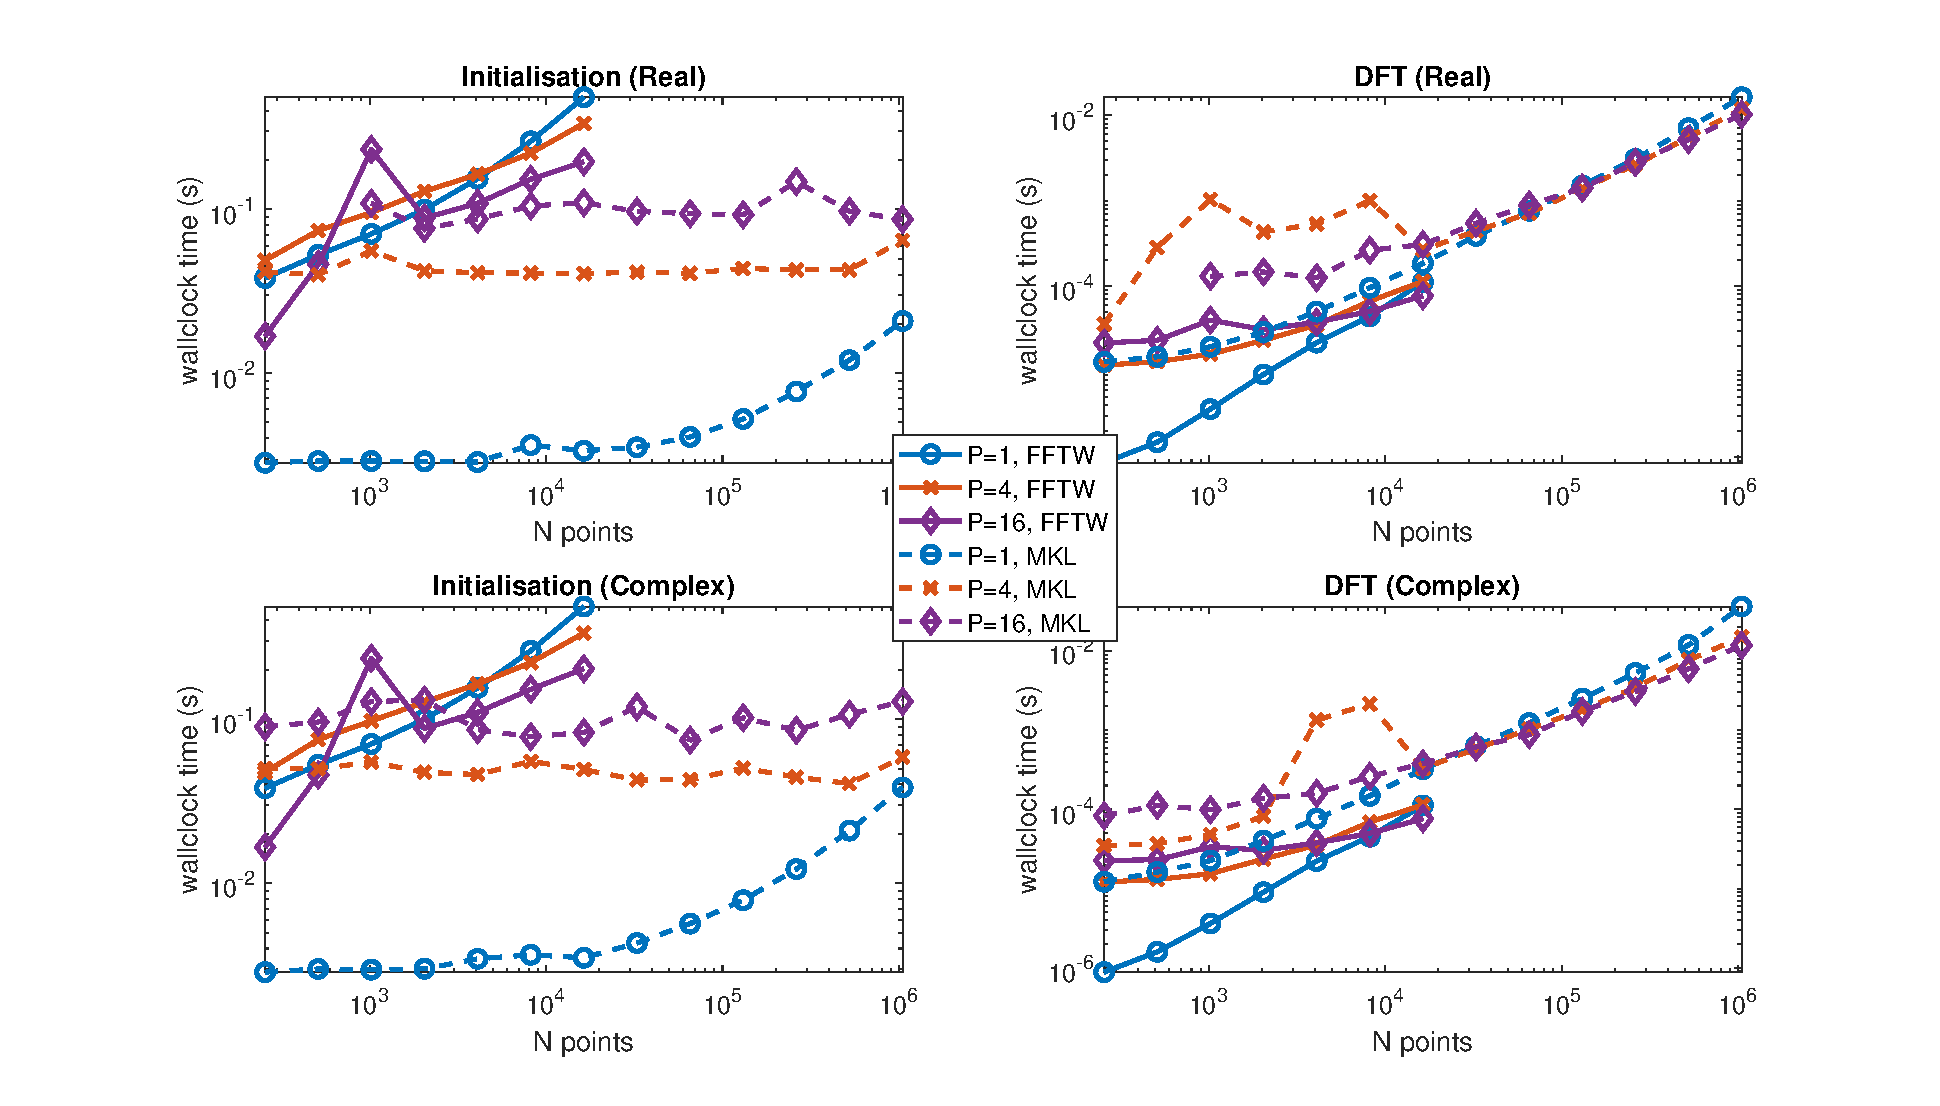
\includegraphics[width=0.9\linewidth]{../results/fftw_mkl_2_1d_mpi.eps}
  \caption{Initialisation and DFT execution times of distributed FFTW and MKL libraries applied to 1D signal as a function of the
    number of points, $N,$ and varying the number of MPI processes, $P,$ with one thread per process. $N$ is a power of 2.}
  \label{1DDistFFTWMKL2}
\end{figure}


\begin{table}
\begin{center}
%\being{small}
\begin{tabular}{|r||r|r|r|r|r|r|r|}
  \hline
 & \multicolumn{7}{|c|}{$thr$} \\
$P$ & 1 & 2 & 4 & 8 & 12 & 16 & 24 \\ \hline
  1 &    2309 &   1868 &  1978 &  2079 &  2904 &  3385 & $\infty$   \\
  2 &     4981 &  7463 &  28941 & $\infty$ &  $\infty$ &           - &           - \\
  4 &     1329 &  4099 &   7575 &           - &          - &          - &          - \\
  8 &    1101 &   2979  &         - &          - &          - &          - &          - \\
  16 &    401 &          - &          - &          - &          - &          - &          - \\ \hline
\end{tabular}
\caption{ For the complex case and $N=16384,$ we provide the minimal value of $l$ such that the overall initialisation time plus time to perform $l$ DFT calculations is lower for FFTW than MKL.  }\label{Tbl:1Dl}
%\end{small}
\end{center}
\end{table}

\clearpage

\section{Effect of domain size and distributed parallelisation for 2D benchmarks}\label{Sec:2DDistr}


In this section, we compare the benchmark results for distributed
libraries that apply the fast Fourier transform to 2D arrays.  The
P3DFFT library cannot be used on 2D problems and, hence, is
excluded. These benchmarks were performed with the MPI-OpenMP versions
of FFTW and MKL. 

As in Section~\ref{Sec:2DMulti}, we set $n_3=4,$ $n_q=4$ and $n_1=n_2=N,$ were $N$ is
defined as follows.  For one set of tests, we let $N=2^k$ for
$k=5,\ldots,12.$ For the other set of tests, $N$ is defined to be the
closest prime number to $2^k,$ $k=5,\ldots,12:$ if two primes are
equidistant, we choose the larger one.

\subsection{2D Distributed FFTW Library}\label{Sec:2DDistFFTW}

Unlike the 1D interface, the 2D interface for the distributed version
of the FFTW library supports both real and complex input
signals. Again, we found that using 12 or 24 MPI processes resulted in
the library crashing when $N$ was a prime number. In
Figure~\ref{2DDistFFTW}, we provide our benchmark results for 1,4 and
16 MPI processes with each process having a single thread. Similarly
to the multithreaded results, for small values of $N,$ the
initialisation times for prime values of $N$ are lower those for
similar values of powers of 2. In general, when $N$ is prime,
increasing the number of processes decreases the initialisation time
but this is not replicated by the results when $N$ is a power of 2,
although the variance in times is much smaller for $N$ a power of
2. The initialisation time increases at a faster rate when $N$ is
prime compared to when $N$ is a power of 2.


\begin{figure}[htb]
    \centering
    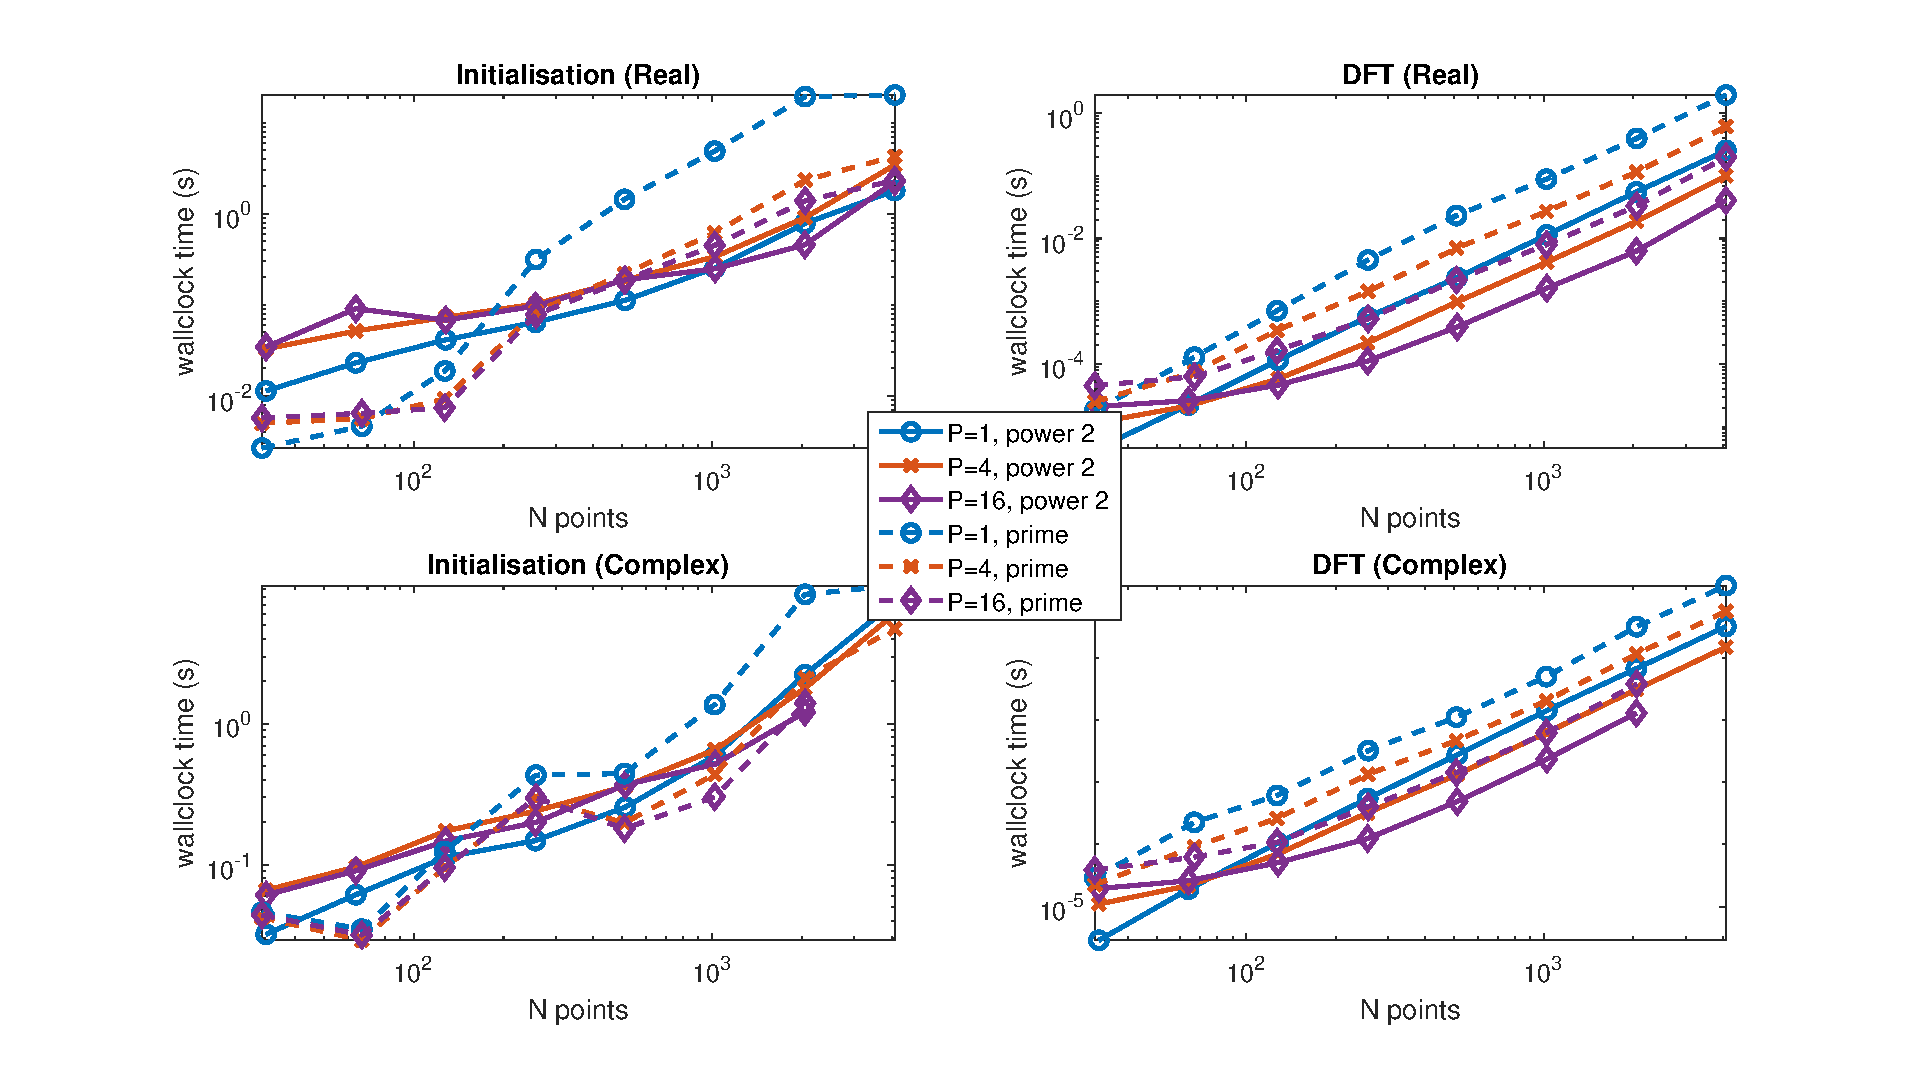
\includegraphics[width=0.9\linewidth]{../results/fftw_2d_mpi.eps}
  \caption{Initialisation and DFT execution times of distributed FFTW library applied to 2D signal as a function of the
    number of points, $N,$ and varying the number of MPI processes, $P,$ with one thread per process.}
  \label{2DDistFFTW}
\end{figure}

Apart from the very smallest values of $N$ considered, increasing the
number of MPI processes always results in a reduction in DFT
calculation time. In Tables~\ref{Tbl:FFTW2d2048},
\ref{Tbl:FFTW2d2048c} and \ref{Tbl:FFTW2d2053}, we provide the data
for $N=2048$ with real input signals, $N=2048$ with complex input
signals, and $N=2053$ with real and complex signals, respectively. For
$N=2048$ with real input signals, 16 MPI processes with single threads
reduces for the DFT time by a factor of 9, and for the complex case it
is reduced by slightly more than a factor of 5 when compared to using
a single MPI process and thread. When $N=2053,$ using 16 MPI processes
with a single thread per process reduces the DFT time by factors of
~12 and ~8 for real and complex signals, respectively. Thus, pure MPI
is having a bigger effect on DFT execution times when $N$ is
prime. This is not altogether surprising because, when $N$ is a power
of 2, the problem is reduced to smaller problems using the Fast
Fourier Transform method.



In Figure~\ref{2DDistFFTW16}, we compare our benchmark results for the
case $P\times thr=16,$ where the number of MPI processes, $P,$ are 1,4
and 16. Again, for small values of $N,$ the initialisation times for
prime $N$ are generally lower than when $N$ is a power of 2,
particularly in the real case. The initialisation times in the complex
case appear to be higher than the real case for $N$ a power of 2: this
is confirmed for the $N=2048$ and $N=2053$ in
Tables~\ref{Tbl:FFTW2d2048} and \ref{Tbl:FFTW2d2048c} and we see that
the difference is roughly a factor of 2. When $N$ is a prime number,
the initialisation times are similar for the real and complex cases,
see Table~\ref{Tbl:FFTW2d2053}. Considering the DFT times, we observe that
16 MPI processes with 1 thread per process is nearly always the best
option out of those considered in Figure~\ref{2DDistFFTW16} and 4 MPI
processes with four threads per process is normally the worse. In
general, across all of the results in the aforementioned tables, the
DFT time is slightly lower for real input signals compared to complex
input signals.


\begin{figure}[htb]
    \centering
    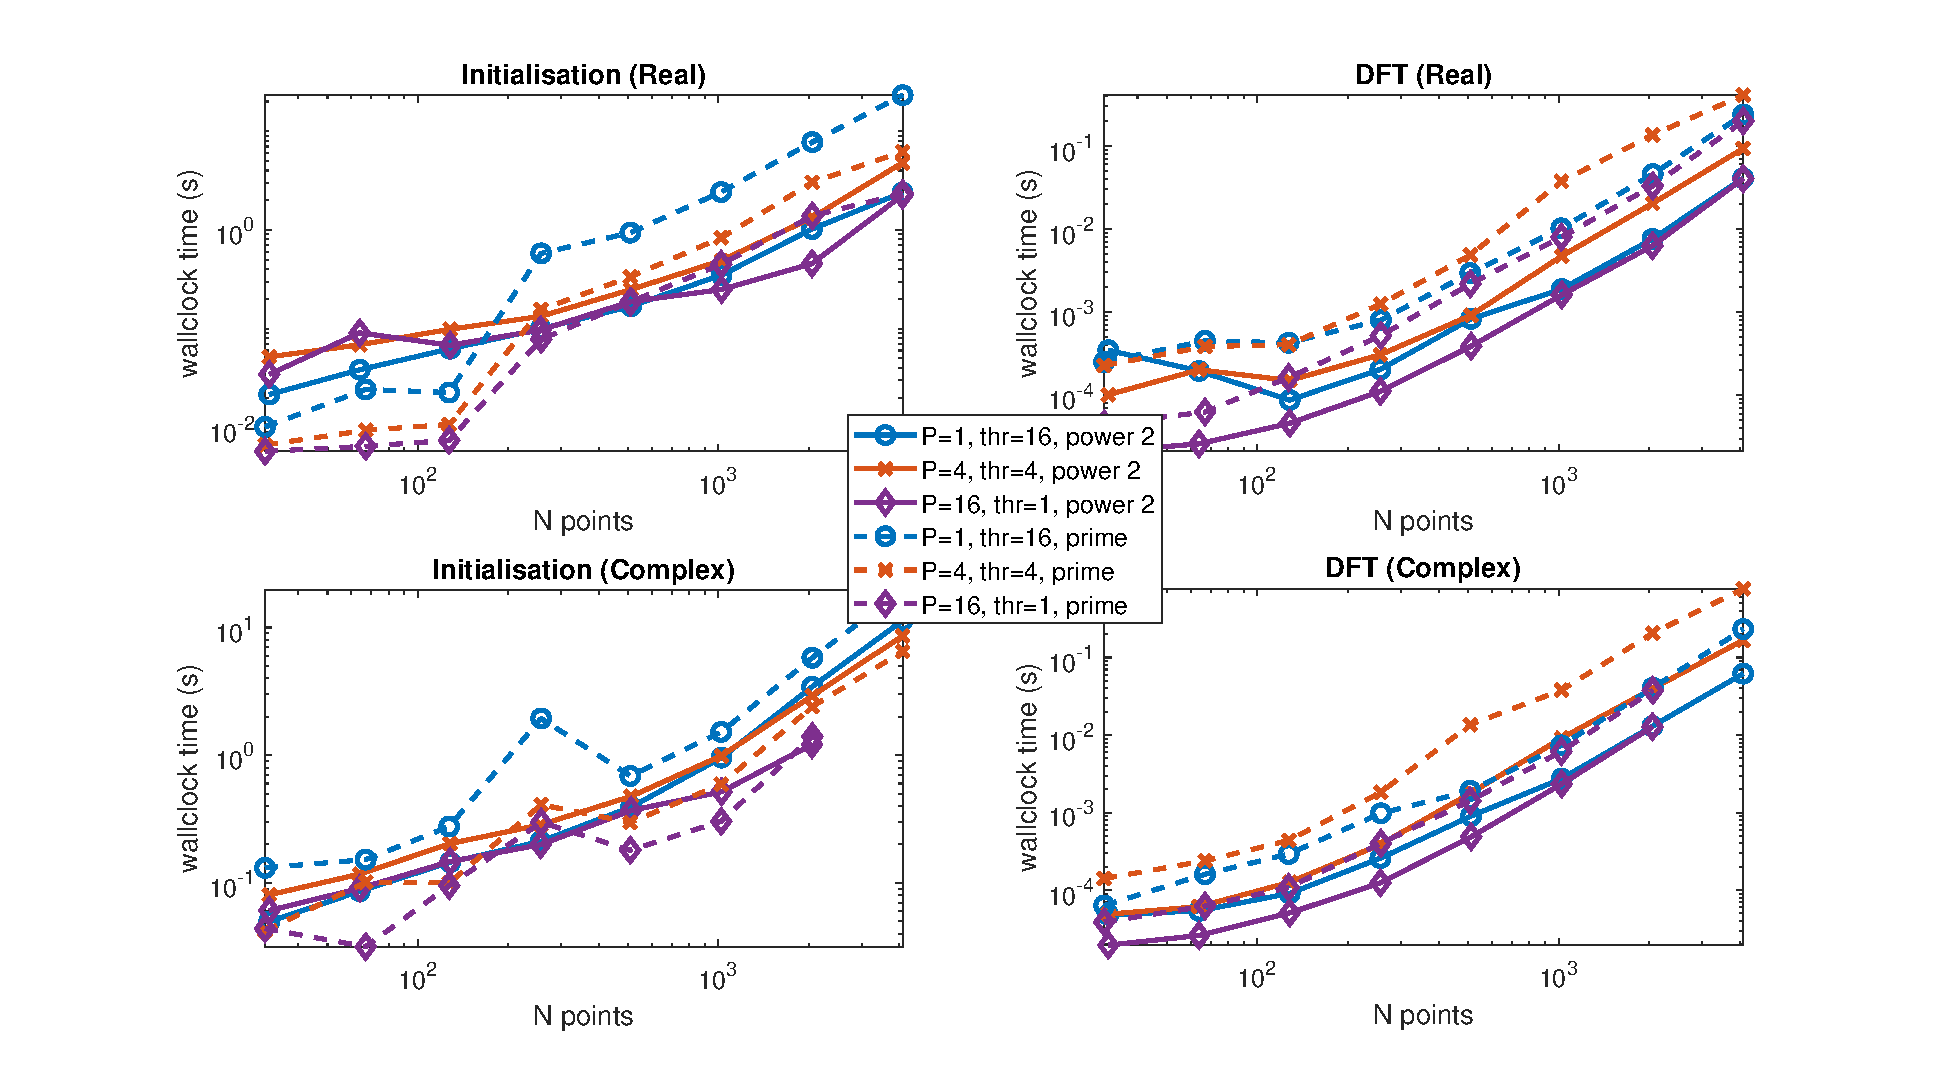
\includegraphics[width=0.9\linewidth]{../results/fftw_2d_mpi_thr.eps}
  \caption{Initialisation and DFT execution times of distributed FFTW library applied to 2D signal as a function of the
    number of points, $N,$ and varying the number of MPI processes, $P,$ and threads, $thr,$ whilst maintaining $P\times thr=16.$}
  \label{2DDistFFTW16}
\end{figure}



\subsection{2D Distributed MKL Library}\label{Sec:2DDistMKL}
The 1D distributed interface to MKL's FFT library did not have
provision for input signals with prime-valued lengths but this is not
the case for the 2D interface. In Figure~\ref{2DDistMKL}, we compare
the wallclock execution times for 1, 4 and 16 MPI processes with one
thread per process. Increasing $N$ but keeping the number of MPI
processes has minimal affect on the initialisation times but we
observe that increasing the number of MPI processes increases with
initialisation time. For $N=2048,$ the initialisation times, relative
to a single process and thread, are a factor of 14.2 and 23.1 times
larger for 4 and 16 MPI processes (single thread per process),
respectively, for real signals (see Table~\ref{Tbl:MKL2d2048}); for
complex input signals the factors are 12.4 and 46.7 (see
Table~\ref{Tbl:MKL2d2048c}). In Table~\ref{Tbl:FFTW2d2053}, we provide
the date for $N=2053:$ for real input signals the initialisation times
increase by a factor of 13.2 and 18.2 for 4 and 16 MPI processes
(single thread per process), respectively, over that for a single
process and thread; for complex input signals, the factors are 11.4
and 48.6, respectively.


\begin{figure}[htb]
    \centering
    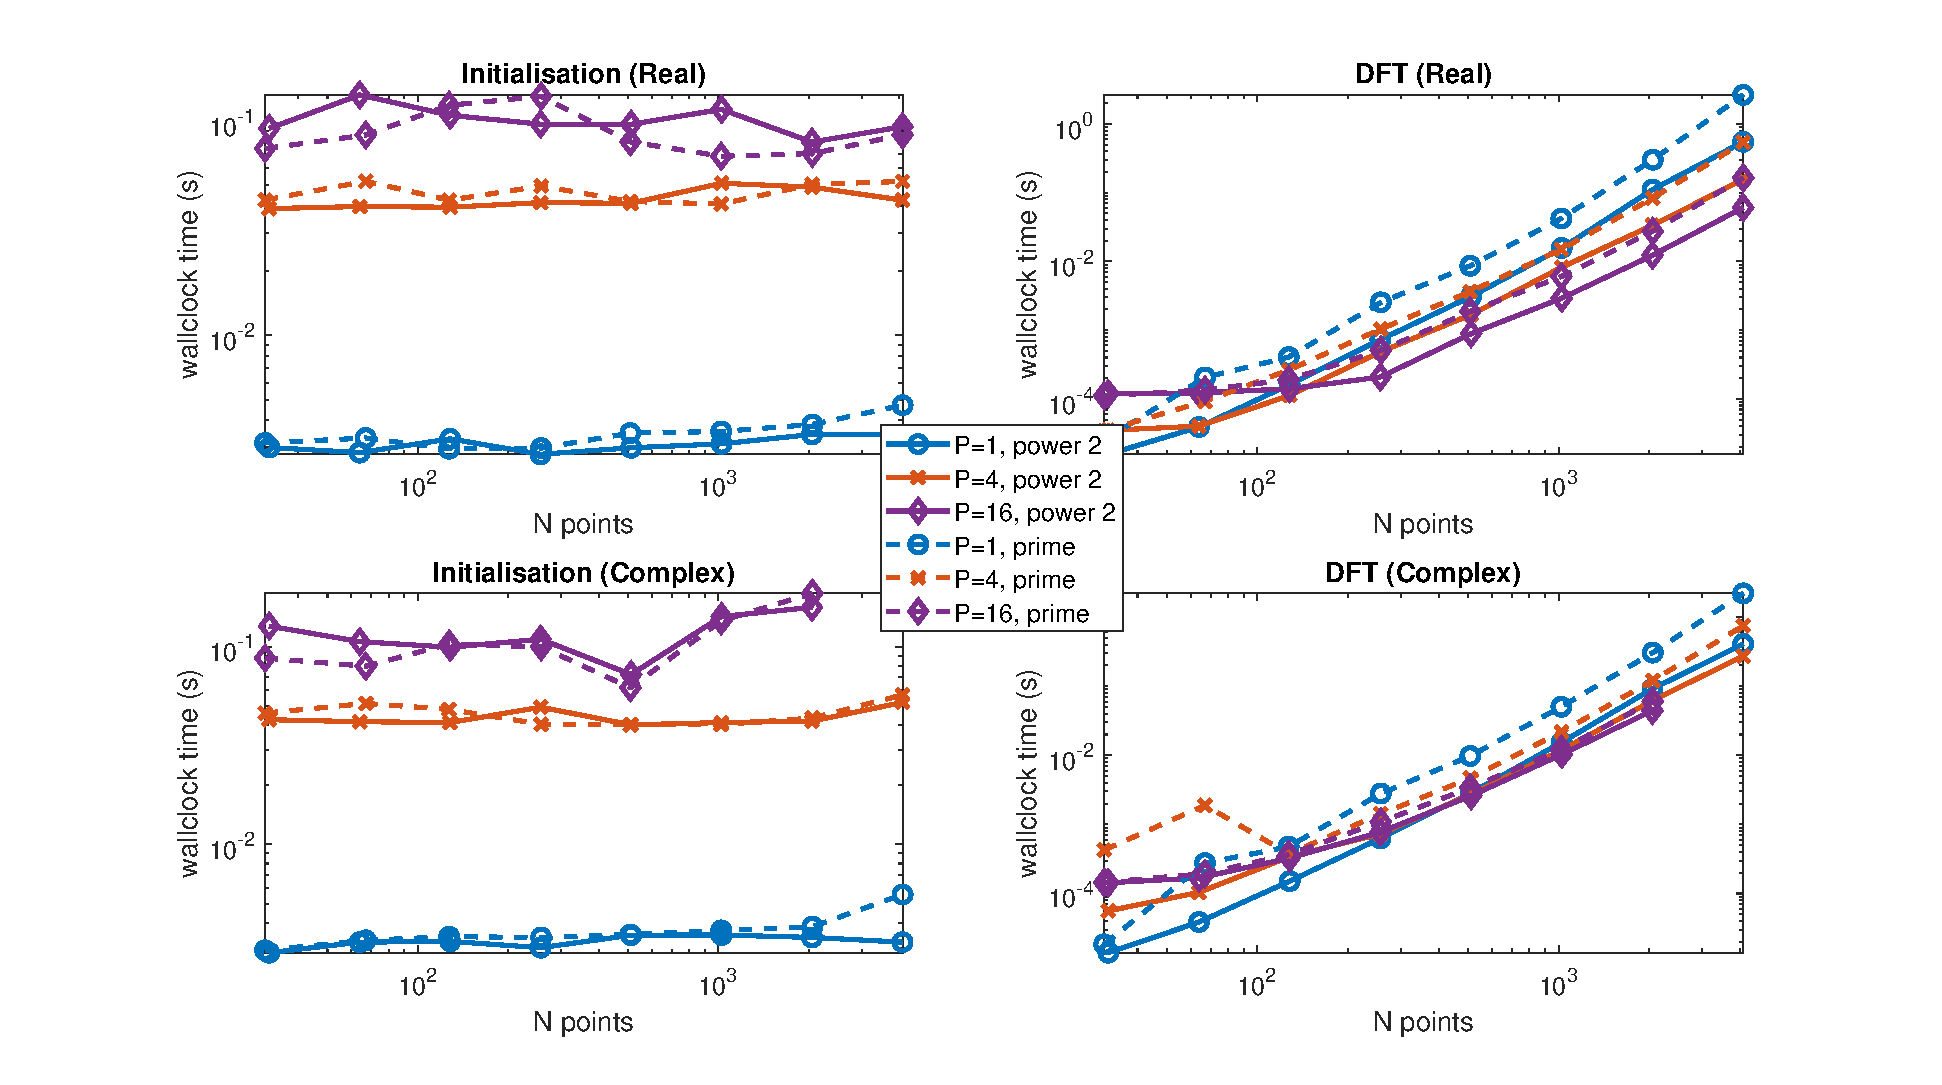
\includegraphics[width=0.9\linewidth]{../results/mkl_2d_mpi.eps}
  \caption{Initialisation and DFT execution times of distributed MKL library applied to 2D signal as a function of the
    number of points, $N,$ and varying the number of MPI processes, $P,$ with one thread per process.}
  \label{2DDistMKL}
\end{figure}

Considering the DFT execution times in Figure~\ref{2DDistMKL}, we
observe that when the input signal is real, in all but the smallest
values of $N,$ increasing the number of processes from 1 to 4 and then
to 16 decreases the execution times: when $N=2048$ the DFT time
decreases by a factor of 3.33 and 9.00 (compared to a single process)
for 4 and 16 MPI processes, respectively (Table~\ref{Tbl:MKL2d2048});
for $N=2053$ the reduction factors are 3.57 and 11.0, respectively
(Table~\ref{Tbl:FFTW2d2053}). Additionally, the DFT execution times
are between 2 and 4 times larger when $N$ is prime compared to $N$
being a power of 2 for similar values of $N.$ For complex input
signals, if $N$ is prime and greater than 128, then we see an
advantage in increasing the number of processes in terms of the DFT
execution time (for $N=2053,$ afactor of 2.53 and 5.06 reduction for 4
and 16 MPI processes, respectively, relative to single process); if
$N$ is a power of 2, then the value of increasing the number of MPI
processes is not so clear from the figure but
Table~\ref{Tbl:MKL2d2048c} reveals that using 4 processes instead of a
single process reduces the DFT time by a factor of 1.47 and if 16
processes is used, then the DFT time is half of that for a single
process.


\begin{figure}[htb]
    \centering
    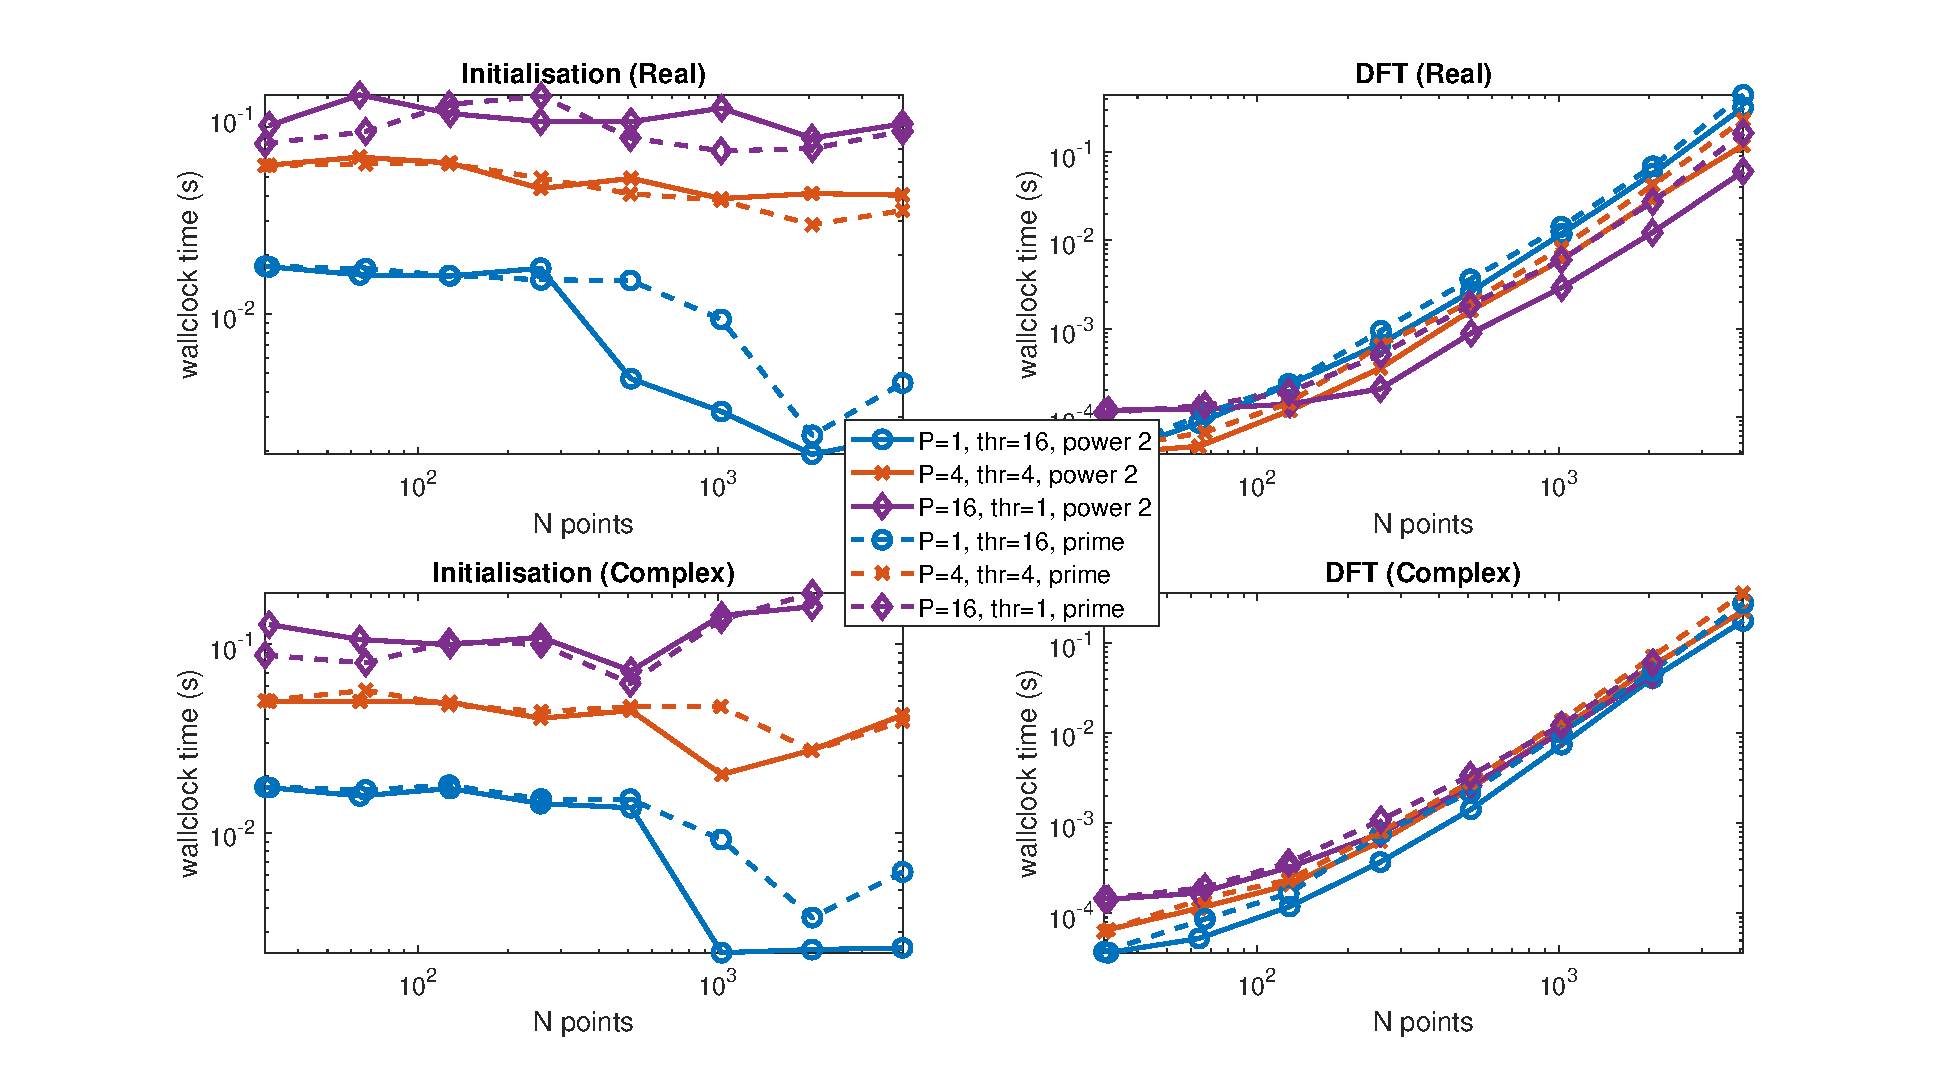
\includegraphics[width=0.9\linewidth]{../results/mkl_2d_mpi_thr.eps}
  \caption{Initialisation and DFT execution times of distributed MKL library applied to 2D signal as a function of the
    number of points, $N,$ and varying the number of MPI processes, $P,$ and threads, $thr,$ whilst maintaining $P\times thr=16.$}
  \label{2DDistMKL16}
\end{figure}

Suppose that, instead of keeping the number of threads per MPI process
as 1, we alter the number of threads such that $P\times thr=16,$ see
Figure~\ref{2DDistMKL16}. For both the real and complex case and the
benchmark results displayed in the figure, using one MPI process with
16 threads is optimal in terms of initialisation times and the
initialisation time drops as $N$ increases. In the figure, increasing
the value of $P$ increases the initialisation time and we do not see a
significant drop as $N$ increases.  Comparing DFT execution times,
when the input signal is real and $N$ is larger than 128, the optimal
times occur when 16 MPI processes with a single thread per process is
used; for the complex case, the optimal choice is one MPI process with
16 threads.





In Table~\ref{Tbl:MKL2d2048}, we see that, across all our benchmark
runs, for $N=2048$ and real input signals, the smallest initialisation
time occured when $P=1$ and $thr=16$ whilst the smallest DFT time was
when $P=16$ and $thr=1:$ considering the time to do a single
initialisation and $k$ DFT calculations and these two combinations of
MPI processes and threads, the total execution time will, on average,
be lower for $P=16$ with $thr=1$ when $k$ is greater than 1.
For
$N=2048$ and complex input signals, $P=1$ with $thr=24$ exhibited the
lowest initialisation and DFT computation times. For $N=2053$
(Table~\ref{Tbl:MKL2d2053}), in both the real and complex cases,
$P=24$ with $thr=1$ exhibits the lowest initialisation time; in the
real case, the lowest DFT time is produced when $P=16$ and $thr=1$
and, in the complex case, $P=1$ with $thr=16$ has the lowest DFT
time. If we consider the total execution time to perform a single
initialisation and $k$ DFT calculations for $N=2053,$ then in the real
case, $P=16$ with $thr=1$ will (on average) outperform $P=1$ with
$thr=24$ for $k\ge 2;$ in the complex case, on average, $P=1$ with
$thr=16$ outperforms $P=1$ with $thr=24$ for all $k\ge 1.$









\subsection{Comparison of distributed libraries for 2D benchmark}\label{Sec:2DDistComp}

We compare the FFTW and MKL 2D distributed interfaces in
Figures~\ref{2DDistFFTWMKL2} and \ref{2DDistFFTWMKLprime} for $N$ a
power of 2 and $N$ a prime number, respectively. For the larger values
of $N,$ MKL outperforms the FFTW library in terms of initialisation
times. When $N$ is a power of 2, the converse is true with respect to
DFT times and, comparing DFT times from Tables~\ref{Tbl:FFTW2d2048}
and \ref{Tbl:MKL2d2048} for real input signals with $N=2048,$ FFTW
takes roughly half the time of MKL. In this case, the average total
time for performing an initialisation followed by atleast 3 DFT
calculations will be lower for FFTW than MKL when $P=24$ and $thr=1.$
For the complex case with $N=2048$ (Tables~\ref{Tbl:FFTW2d2048c} and
\ref{Tbl:MKL2d2048c}), FFTW will, on average, outperform MKL when
doing a single initialisation and at least 8 DFT calculations for
$P=24$ and $thr=1.$ When $N$ is prime and has real input signals, MKL
is outperforming FFTW in terms of DFT execution times although the two
libraries are generally fairly comparable. Therefore, for real input
signals when $N$ is large and prime, we recommend using the MKL
library because of the significant reduction in initialisation
times. For complex signals with $N$ prime, the DFT execution times for
$P=1$ and $P=4$ are very similar for both libraries but FFTW is close
to half the execution time of MKL when $P$ is larger: for $N=2053$
with complex input signal and $P=16,$ the average total time for
performing a single initialisation and $k$ DFT calculations will be
lowest for FFTW once $k>54.$ 


\begin{figure}[htb]
    \centering
    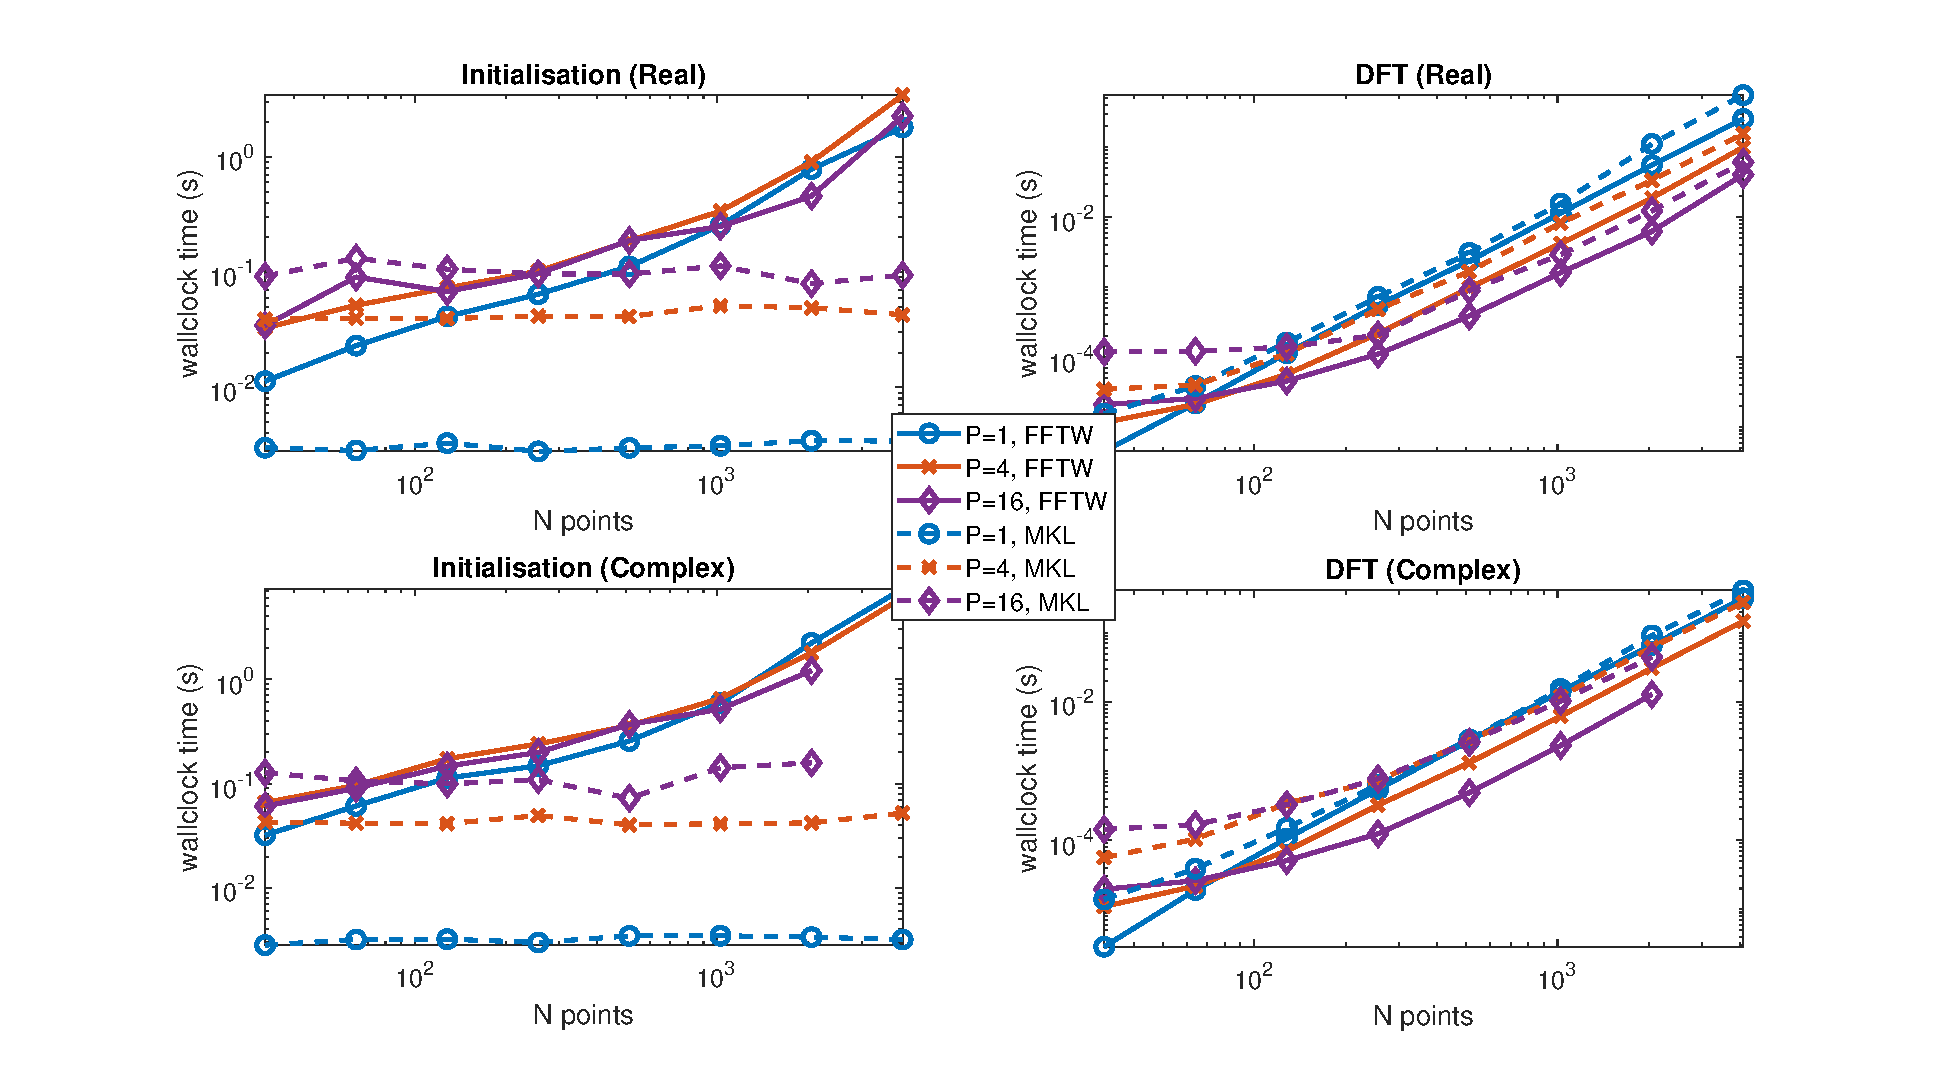
\includegraphics[width=0.9\linewidth]{../results/fftw_mkl_2_2d_mpi.eps}
  \caption{Initialisation and DFT execution times of distributed FFTW and MKL libraries applied to 2D signal as a function of the
    number of points, $N,$ and varying the number of MPI processes, $P,$ with one thread per process. $N$ is a power of 2.}
  \label{2DDistFFTWMKL2}
\end{figure}


\begin{figure}[htb]
    \centering
    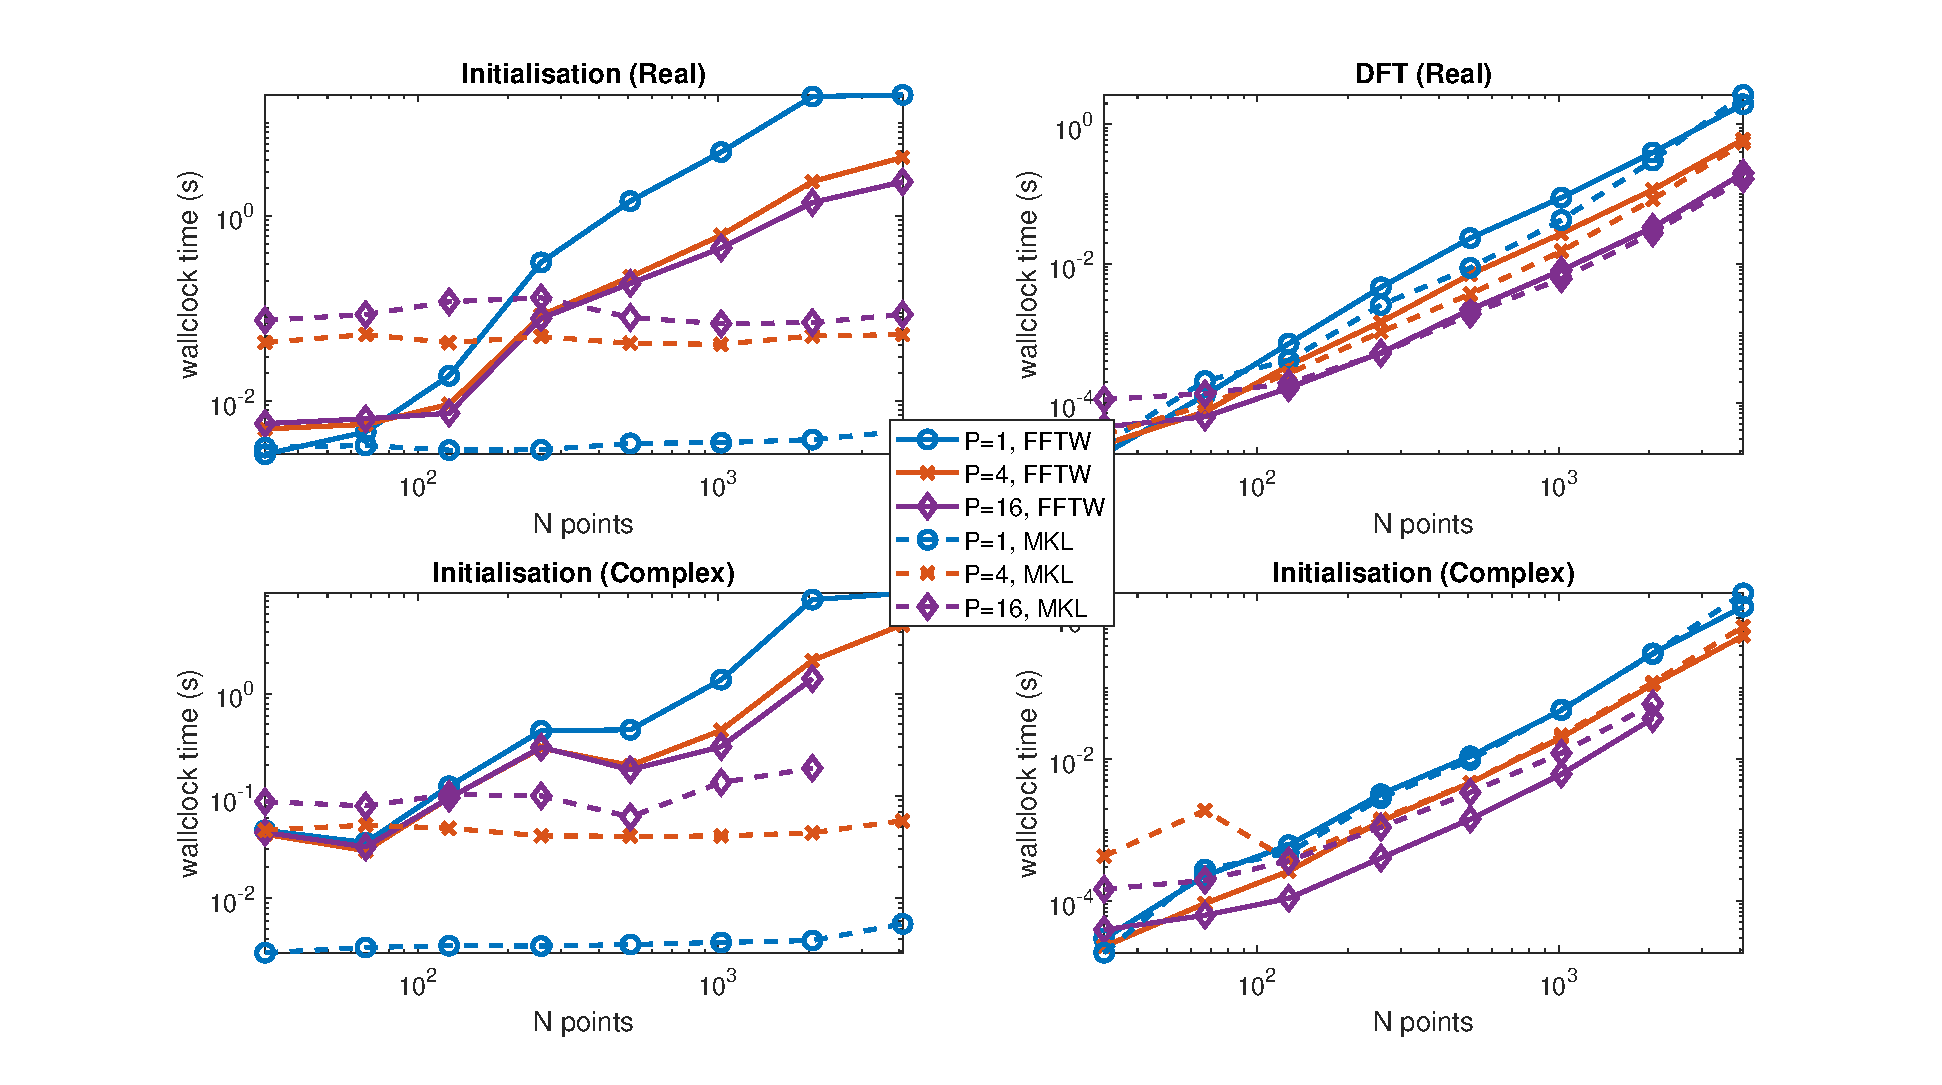
\includegraphics[width=0.9\linewidth]{../results/fftw_mkl_prime_2d_mpi.eps}
  \caption{Initialisation and DFT execution times of distributed FFTW and MKL libraries applied to 2D signal as a function of the
    number of points, $N,$ and varying the number of MPI processes, $P,$ with one thread per process. $N$ is a prime number.}
  \label{2DDistFFTWMKLprime}
\end{figure}



\clearpage

\section{Effect of domain size and distributed parallelisation for 3D benchmarks}\label{Sec:3DDistr}
For 3D problems, we will compare distributed versions of the FFTW, MKL
and P3DFFT libraries. As in Section~\ref{Sec:3DMulti}, we set
$n_q=4$ and $n_1=n_2=n_3=N,$ were $N$ is defined as follows.  For one set
of tests, we let $N=2^k$ for $k=3,\ldots,9.$ For the other set of
tests, $N$ is defined to be the closest prime number to $2^k,$
$k=3,\ldots,9:$ if two primes are equidistant, we choose the larger
one.


\subsection{3D Distributed FFTW Library}\label{Sec:3DDistFFTW}
The FFTW library provides interfaces for both real and complex 3D
signals. In Figure~\ref{3DDistFFTW}, we compare the initialisation and
DFT execution times for varying values of $N$ with 1, 4 and 16 MPI
processes, where each process uses a single thread. As $N$ increases,
the initialisation times increase and we observe that when $P=1,$ the
initialisation times are generally larger when $N$ is prime compared
to when $N$ is a power of 2 but for $P=4$ or 16, the converse is
true. For some of the larger values of $N,$ we ran out of memory on
the node. In Tables~\ref{Tbl:FFTW3d256} and \ref{Tbl:FFTW3d256c}, we
provide the benchmark data for $N=256$ with real and complex input
signals, respectively. The benchmark data for $N=257$ is provided in
Table~\ref{Tbl:FFTW3d257}. We observe that for $N=256$ the
initialisation times for the complex case with $thr=1$ are roughly
double those of the real case. For $N=257,$ there is no consistant
behaviour when comparing the intialisation times for real and complex
input signals with $thr=1.$



\begin{figure}[htb]
    \centering
    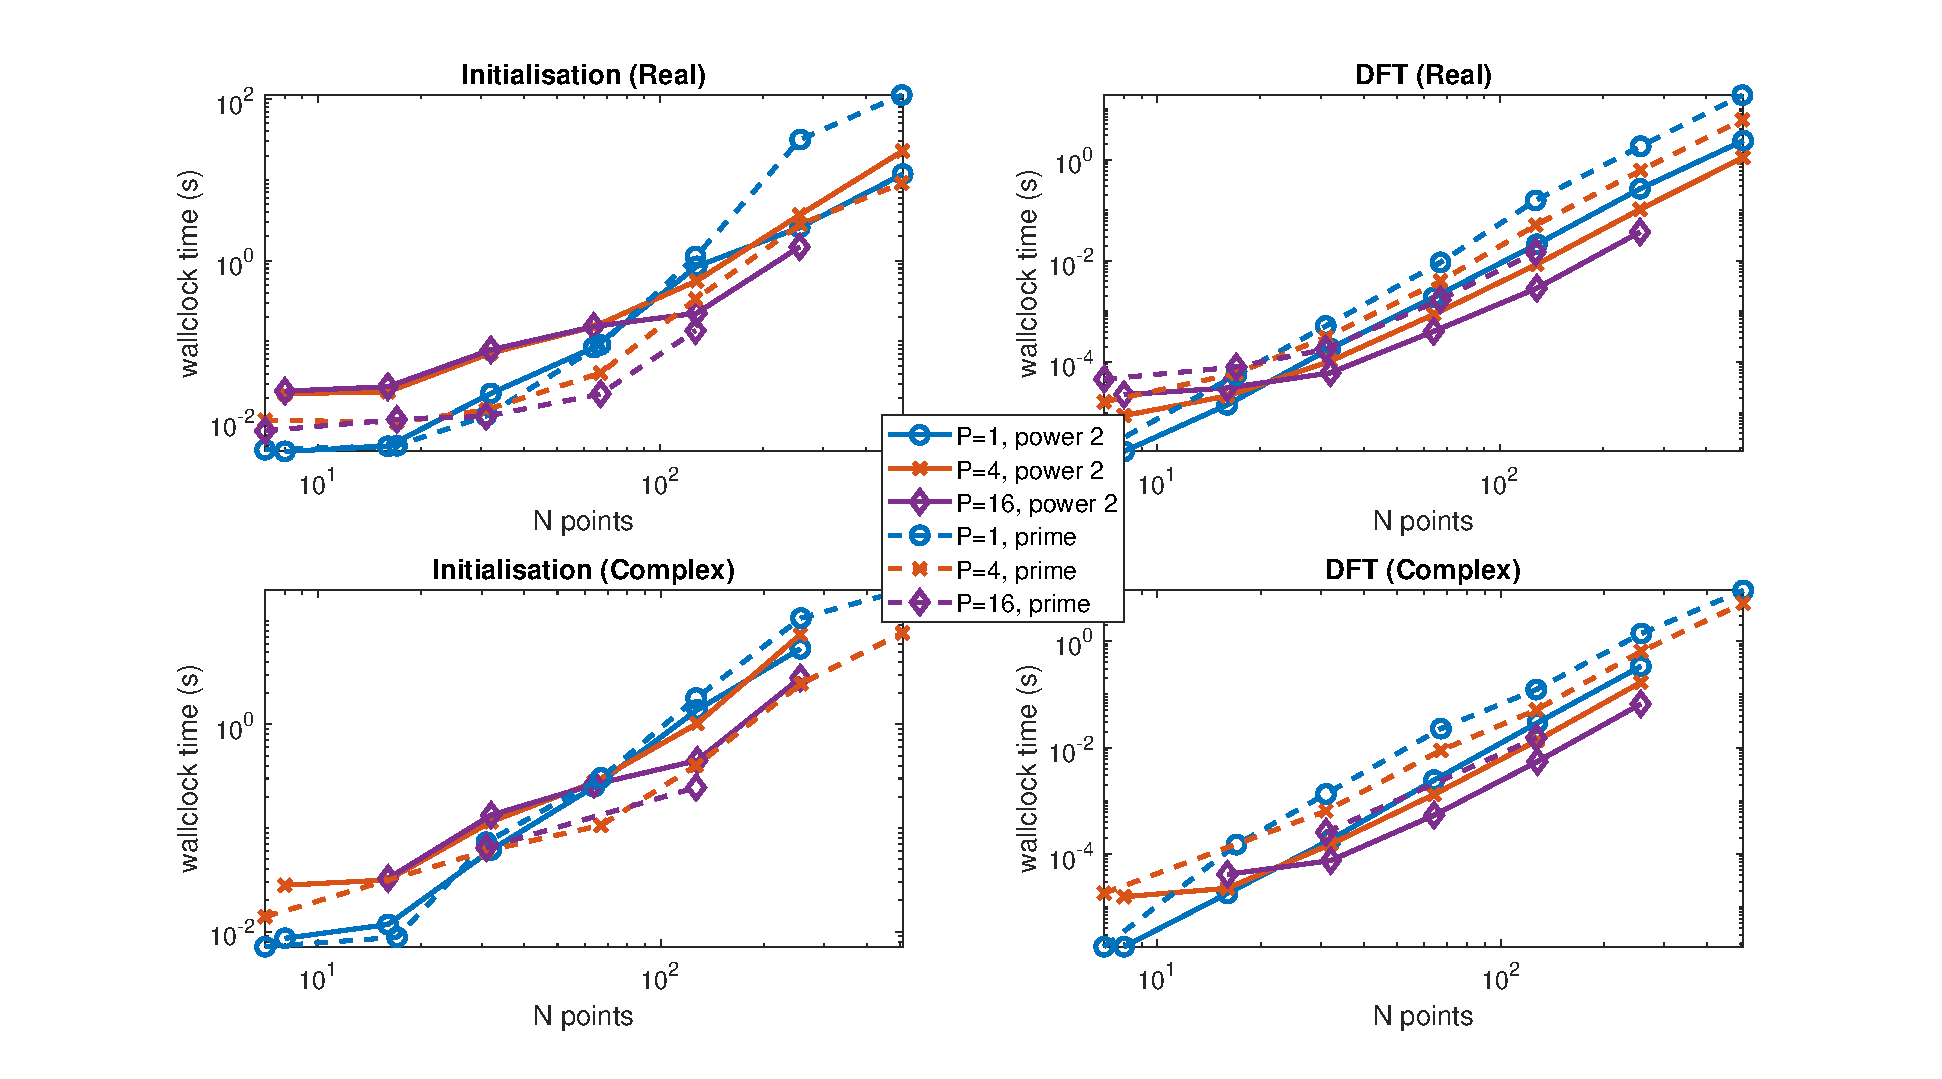
\includegraphics[width=0.9\linewidth]{../results/fftw_3d_mpi.eps}
  \caption{Initialisation and DFT execution times of distributed FFTW library applied to 3D signal as a function of the
    number of points, $N,$ and varying the number of MPI processes, $P,$ with one thread per process.}
  \label{3DDistFFTW}
\end{figure}

Looking at the DFT execution times in Figure~\ref{3DDistFFTW}, for $N$
greater than 120, increasing $P$ from 1 to 4 to 16 decreases the times
for both the real and complex input signals. The execution times for
prime values of $N$ are significantly larger for $N$ a prime number
compared to $N$ a power of 2. From Tables~\ref{Tbl:FFTW3d256} and
\ref{Tbl:FFTW3d257}, we see that in the real case, the DFT execution
times with $thr=1$ are between 4.9 and 6.9 times larger for $N=257$
compared to $N=256.$ For complex signals with $thr=1,$ the DFT
execution times are between 3.1 and 4.2 times larger for $N=257$
compared to $N=256,$ see Tables~\ref{Tbl:FFTW3d256c} and
\ref{Tbl:FFTW3d257}.

\begin{figure}[htb]
    \centering
    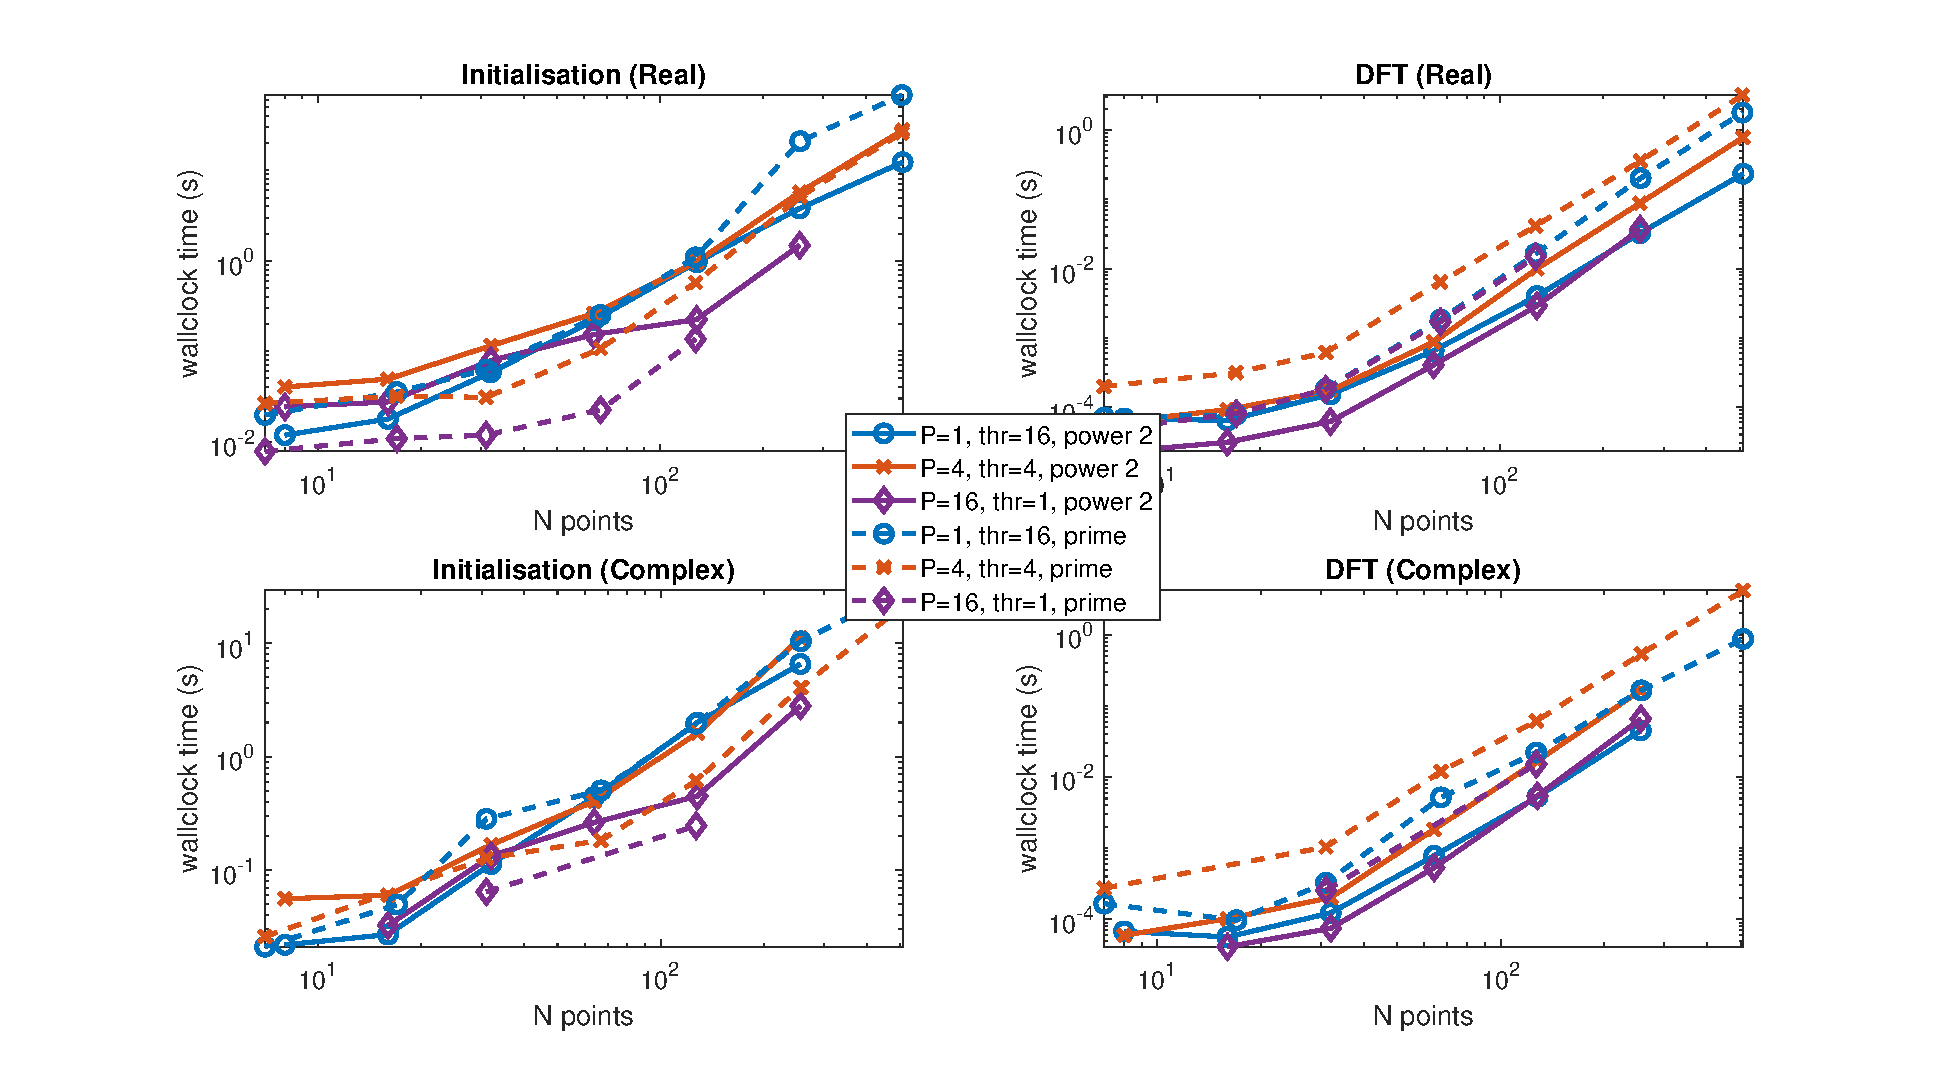
\includegraphics[width=0.9\linewidth]{../results/fftw_3d_mpi_thr.eps}
  \caption{Initialisation and DFT execution times of distributed FFTW library applied to 3D signal as a function of the
    number of points, $N,$ and varying the number of MPI processes, $P,$ and threads, $thr,$ whilst maintaining $P\times thr=16.$}
  \label{3DDistFFTW16}
\end{figure}


In Figure~\ref{3DDistFFTW16} we compare the initialisation and DFT
execution times for $P\times thr=16,$ where $P=1,$ 4 and 16. For $N$ a
power of 2, setting $P=4$ and $thr=4$ is the worse combination with
respect to DFT execution times for both classes of $N.$ In terms of
intialisation times, when $N$ is a power of 2, the combination $P=4$
and $thr=4$ also has the highest times for those combinations
considered in the figures; for $N$ prime, $P=1$ and $thr=16$ has the
worse initialisation times and increasing $P$ reduces the time.

Looking at all the data in Table~\ref{Tbl:FFTW3d256}, we see that when
$N=256$ and the input signal is real, the best DFT time occurs when
$P=1$ and $thr=24$ whilst the best initialisation time is when $P=24$
and $thr=1.$ Comparing the average time to perform a single
initialisation and $k$ DFT calculations for these two combinations, if
$k$ is smaller than 94, then $P=24$ and $thr=1$ is best but, for larger
values of $k,$ the user should switch to $P=1$ and $thr=24.$ For
$N=256$ with complex input signals, from Table~\ref{Tbl:FFTW3d256c} we
observe that the best DFT execution time occurs when $P=1$ and
$thr=16$ but the best initialisation time is when $P=16$ and $thr=1.$
Comparing these two combinations when performing a single
initialisation and $k$ DFT calculations, we find that the average time
is better for $P=16$ and $thr=1$ when $k<183$ but $P=1$ and $thr=16$
is optimal for larger values of $k.$

For $N=257,$ we see from Table~\ref{Tbl:FFTW3d257} that for both the
real and complex cases, the smallest initialisation time occurs when
$P=8$ and $thr=1$ and the smallest DFT execution time has $P=1$ and
$thr=24.$ As above, we compare the two combinations with respect to
the total (average) time to perform a single initialisation and $k$
DFT calculations. In the real case, $P=8$ and $thr=1$ is lower when
$k<72$ but $P=1$ and $thr=24$ is the better combination for larger
values of k; for the complex case, $P=8$ and $thr=1$ has lower total
time for $k<45,$ whilst $P=1$ and $thr=24$ has lower total time for
$k\ge 45.$



\subsection{3D Distributed MKL Library}\label{Sec:3DDistMKL}
In Figure~\ref{3DDistMKL}, we compare the distributed MKL FFT library
for different values of $N$ with $P=1,$ 4 and 16 with each MPI process
using a single thread. The initialisation times for $N$ a power of 2
and $N$ prime. Interestingly, the behaviour for $P=1$ and real input
signals is vastly different to that when the input signal is
complex. It is also different to the multithreaded version of the MKL
library with a single thread being used. Here, for $P=1$ and real
input signal, increasing $N$ beyond 64 leads to significant increases
in initialisation time as $N$ grows. We also start to see the
initialisation times for $P=4$ and real input signals starting to
increase for $N$ larger than 200. For the smaller values of $N$ and
real signals, increasing the number of MPI processes appears to, in
general, increase the initialisation times for both real and complex
input signals (this is also true for the larger values of $N$ in the
complex case). The benchmark data for $N=256$ is provided in
Tables~\ref{Tbl:MKL3d256} (real) and \ref{Tbl:MKL3d256c} (complex). We
observe that for $P=1$ and $thr=1$, the initialisation time in the
real case is 18 times larger than the complex case and increasing $P$
whilst keeping $thr=1$ results in the difference becoming smaller:
when $P=24$ the initialisation times are similar. The benchmark data
for $N=257$ is available in Table~\ref{Tbl:MKL3d257} and we observe
similar behaviour.

\begin{figure}[htb]
    \centering
    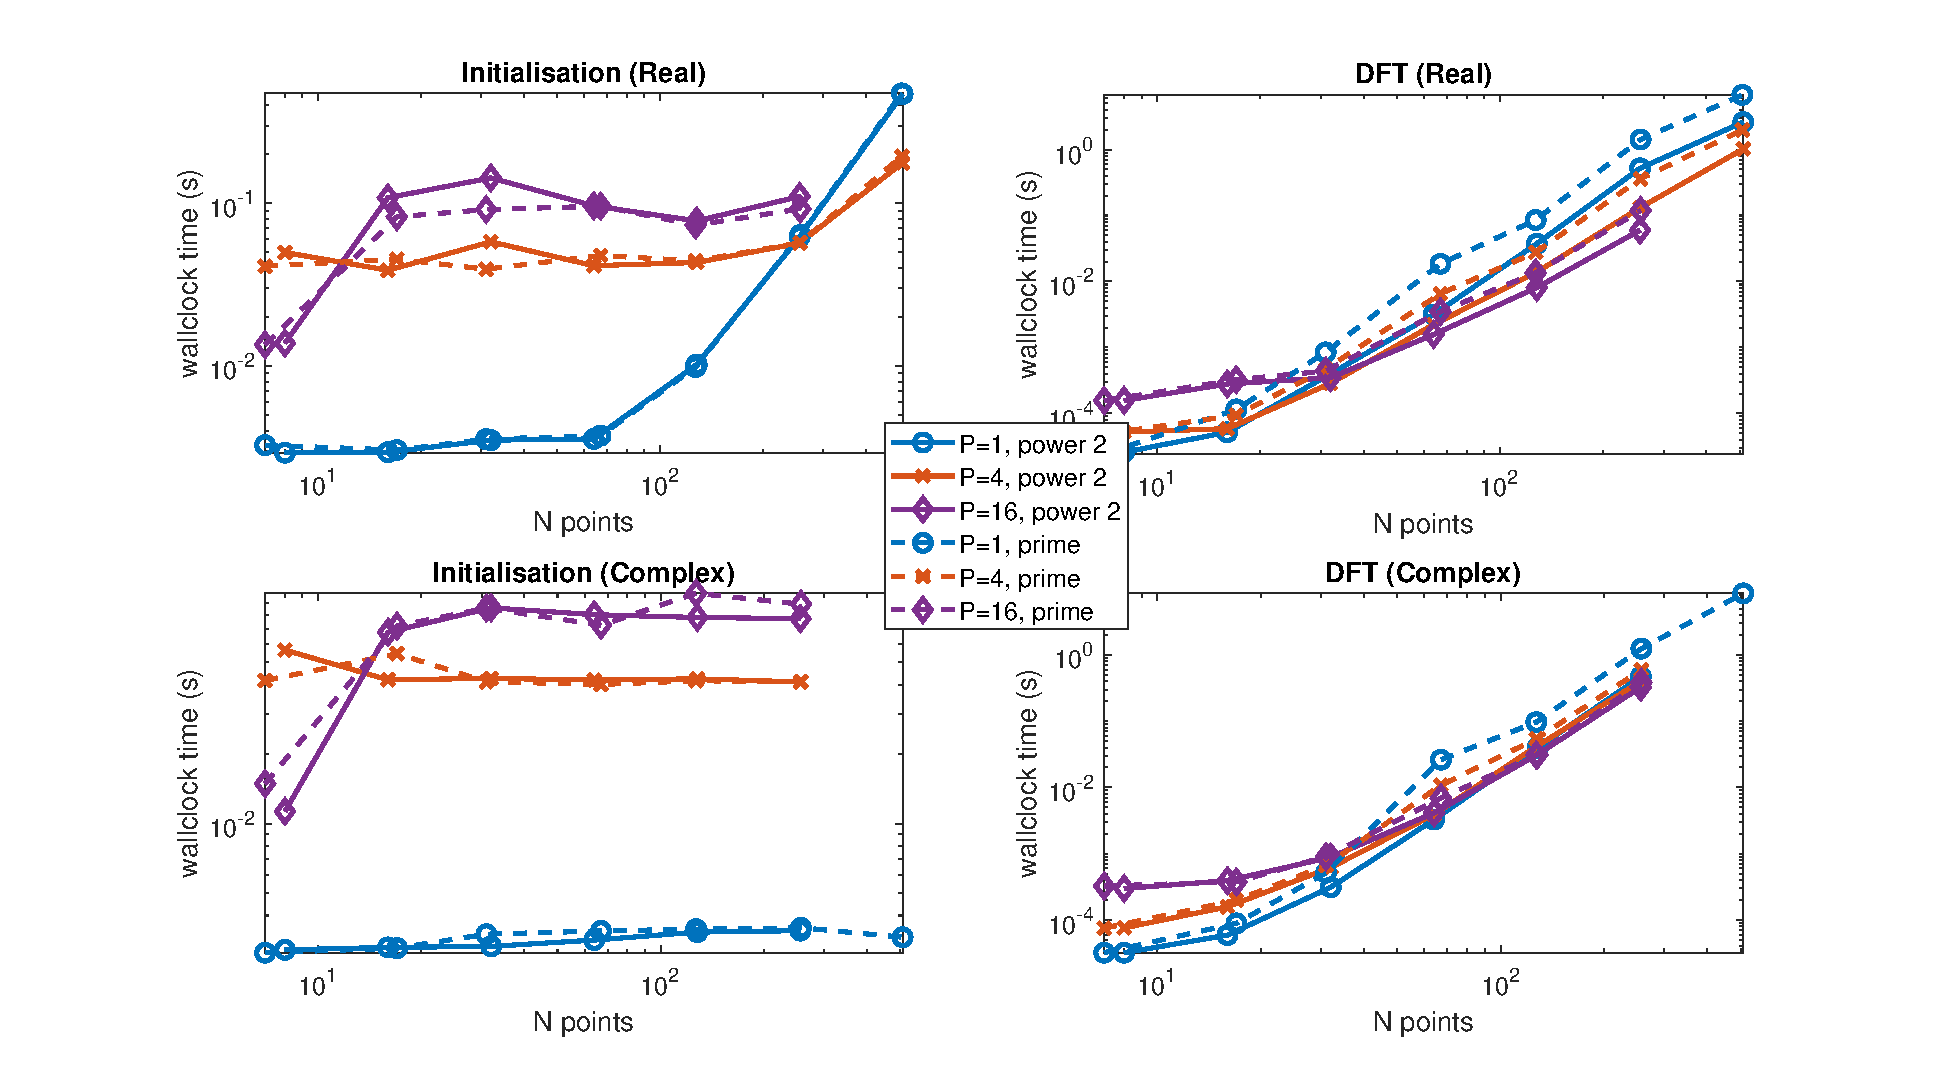
\includegraphics[width=0.9\linewidth]{../results/mkl_3d_mpi.eps}
  \caption{Initialisation and DFT execution times of distributed MKL library applied to 3D signal as a function of the
    number of points, $N,$ and varying the number of MPI processes, $P,$ with one thread per process.}
  \label{3DDistMKL}
\end{figure}

For the DFT execution times, we see differing behaviour between the
real and complex cases, Figure~\ref{3DDistMKL}. For the real case, 16
MPI processes is suboptimal for small values of $N$ but for $N\ge 64$
it exhibits the lowest execution times for the three values of $P$
considered in the figure. Additionally, the DFT execution times are
lower when $N$ is a power of 2 compared to when it is prime: from
Tables~\ref{Tbl:MKL3d256} and \ref{Tbl:MKL3d257}, we find that there
is between a factor of 2 and 3 difference for $thr=1.$ Considering the
complex case, as $N$ increases, when $P=4$ or 16, the DFT execution
times appear to be similar for both $N$ a power of 2 and $N$
prime. However, when analysing the data in Tables~\ref{Tbl:MKL3d256c}
and \ref{Tbl:MKL3d257} for $N=256$ and 257, respectively, (with
$thr=1$) we see that the latter is 50\% larger for $P=4$ and 20\%
larger for $P=16.$ The results for $N=257$ have better strong
scalability with respect to $P$ when $thr=1$ than when $N=256.$ When
comparing the real and complex strong scalability results ($fratio$),
we see that for both $N=256$ and $N=257$ that the real case is
exhibiting better scalabiling than the complex case.




\begin{figure}[htb]
    \centering
    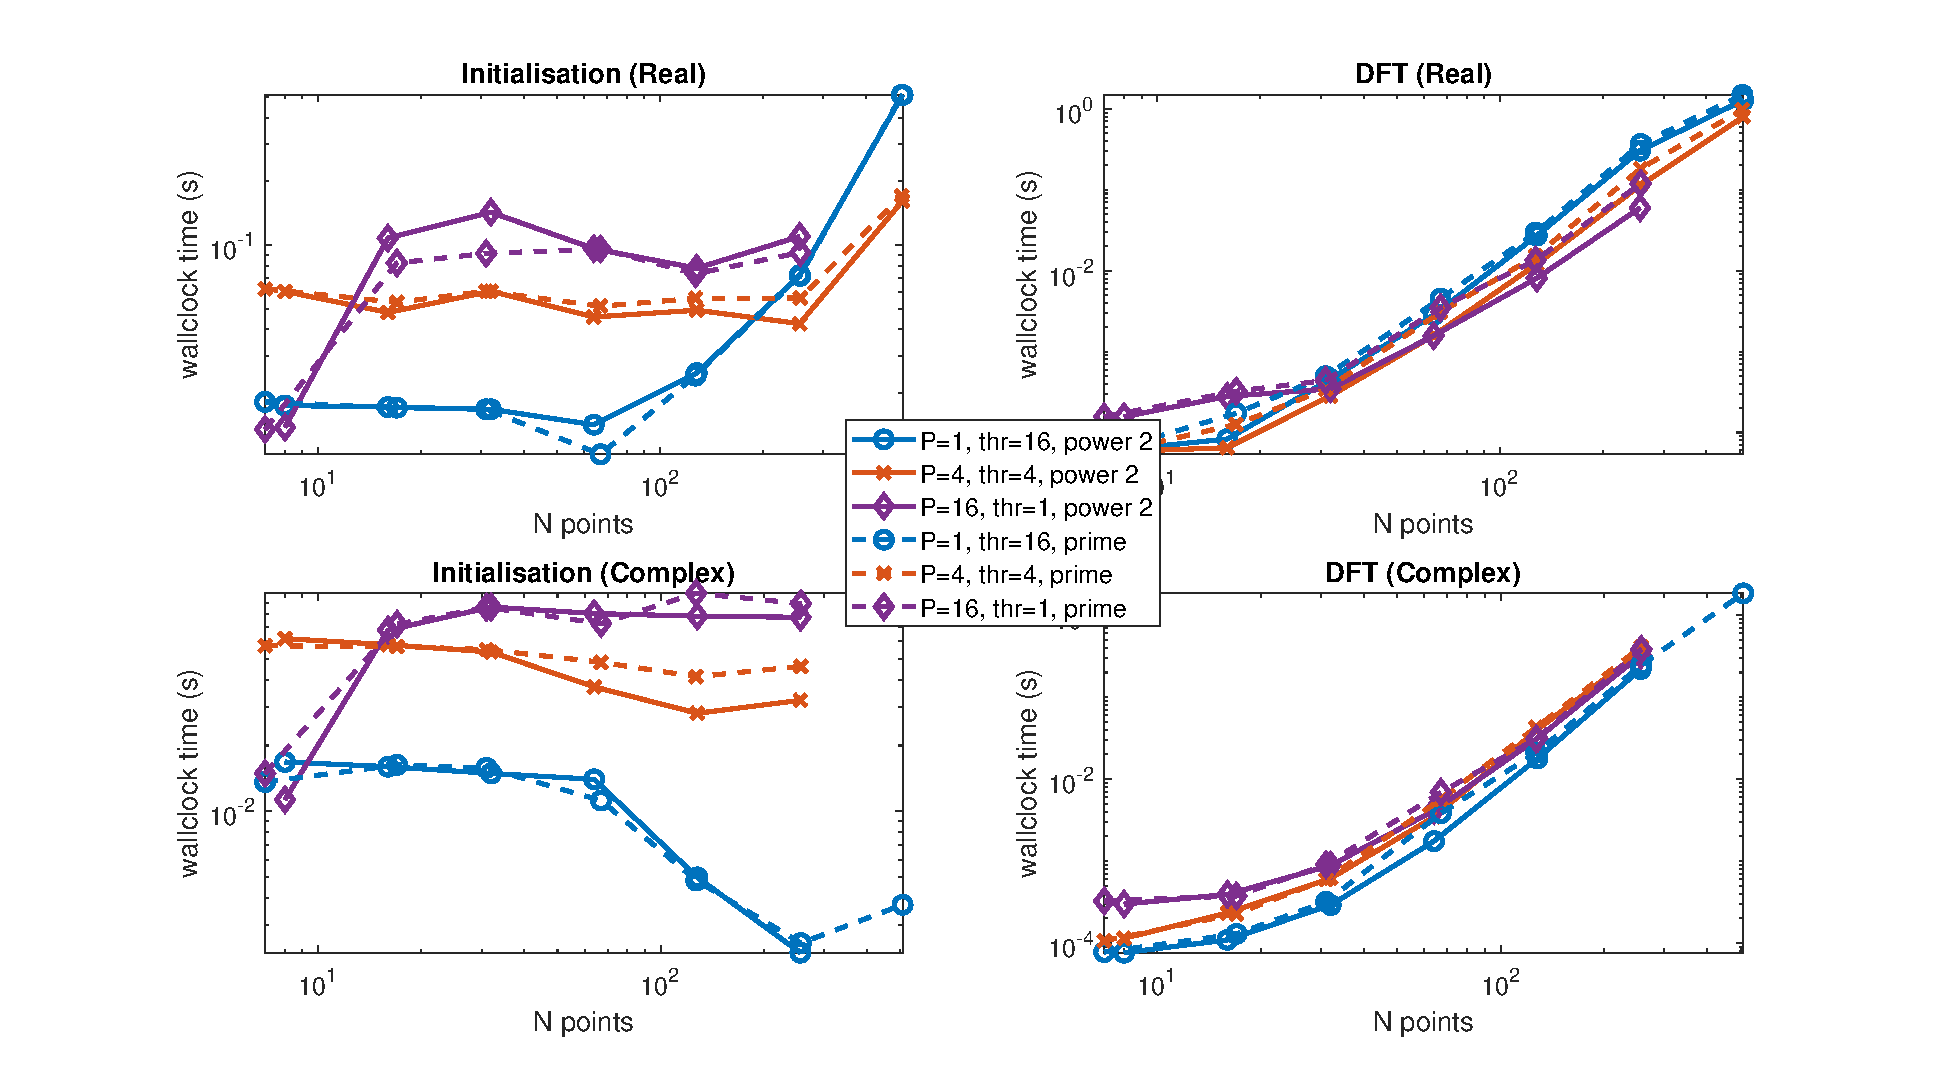
\includegraphics[width=0.9\linewidth]{../results/mkl_3d_mpi_thr.eps}
  \caption{Initialisation and DFT execution times of distributed MKL library applied to 3D signal as a function of the
    number of points, $N,$ and varying the number of MPI processes, $P,$ and threads, $thr,$ whilst maintaining $P\times thr=16.$}
  \label{3DDistMKL16}
\end{figure}

In Figure~\ref{3DDistMKL16}, we compare the results for
$P\times thr=16$ for $P=1,$ 4 and 16. As before, the behaviour of the
initialisation times for $P=1$ and $thr=16$ differs between the real
and complex input cases: in the real case, increasing $N$ beyond 100
increases the initialisation time but for the complex case the
initialisation time decreases. This is highlighted when we see that
real to complex ratio of the initialisation time for $N=256,$ $P=1$
and $thr=16$ is 32.0 (Tables~\ref{Tbl:MKL3d256} and
\ref{Tbl:MKL3d256c}) but for the same value of $N$ with $P=4$ and
$thr=4$ we have a ratio of 3.19. For the $P=4$ and 16, increasing the
size of $N$ is, in general, having little effect on the initialisation
time. The log-log axis for the DFT execution times mean that the
differences in times are hard to see. For real input signals, the
ratios for $N=257$ versus $N=256$ are 1.21, 1.62 and 1.99 for $P=1,$ 4
and 16, respectively; for complex signals the ratios are 1.12, 1.15
and 1.17, respectively. Let $N=256$ then, for $P=1$ with $thr=16,$ the
complex to real ratio of the average DFT execution time is 0.72, for
$P=4$ with $thr=4$ the ratio is 3.19, and for $P=16$ with $thr=1$ the
ratio is 5.44 (Tables~\ref{Tbl:MKL3d256} and
\ref{Tbl:MKL3d256c}). Considering $N=257,$ the complex to real ratio
of the average DFT execution time is 0.67 for $P=1$ with $thr=16,$
2.26 for $P=4$ with $thr=4,$ and 3.22 for $P=16$ with $thr=1$
(Table~\ref{Tbl:MKL3d257}).

Looking at the data in Table~\ref{Tbl:MKL3d256}, for real input
signals with $N=256,$ the optimal choice for $P$ and $thr$ is $P=4$
with $thr=4$ with respect to initialisation time and $P=16$ with
$thr=1$ with respect to DFT execution time. Suppose that a single
initialisation is followed by $k$ DFT calculations, then, on average,
$P=16$ with $thr=1$ will outperform $P=4$ with $thr=4$ for all $k>1.$
For $N=256$ and the complex case (Table~\ref{Tbl:MKL3d256c}), $P=1$
with $thr=24$ outperforms the other combinations with respect to both
initialisation and DFT execution times. For real input signals with
$N=257,$ $P=8$ with $thr=2$ has the lowest initialisation time and
$P=16$ with $thr=1$ has the best DFT execution time
(Table~\ref{Tbl:MKL3d257}). Comparing the total (average) time to
perform a single initiailisation and $k$ DFT executions, the latter
combination is faster for all $k\ge 3.$ For $N=257$ and complex input
signals, $P=1$ with $thr=24$ is optimal with respect to initialisation
time and $P=1$ with $thr=16$ is optimal with respect to DFT execution
time: the latters total time to perform a single initialisation and
$k$ DFT executions is best for all $k>0.$





\subsection{3D Distributed P3DFFT Library}\label{Sec:3DDistP3DFFT}

As mentioned earlier on, the P3DFFT library is restricted to real
input signals. In Figure~\ref{3DDistP3DFFT}, we compare the
initialisation and DFT executions for $N$ a power of 2 and $N$ prime,
and use $P$ MPI processes, $P=1,$ 4 and 16, with 1 OpenMP thread,
$thr.$ Increasing $N$ increases both the initialisation and DFT
execution times for all values of $P$ considered in the figure. For
$N\le 32,$ increasing $P$ is showing little effect on the
initialisation time. For larger values of $N,$ we see that increasing
the number of MPI processes is decreasing the initialisation time. In
Table~\ref{Tbl:P3DFFT3d256}, we provide the benchmark data for
$N=256.$ We see that, in general, increasing $P$ decreases the
initialisation time for all values of $thr$ considered. For $P=16$ and
$thr=1,$ there has been an 85\% reduction in initialisation time
compared to $P=1$ and $thr=1.$ The benchmark data for $N=257$ is
provided in Table~\ref{Tbl:P3DFFT3d257} and we see that increasing $P$
but keeping $thr$ constant results in a reduction in initialisation
time with an 85\% reduction when switching from $P=1$ with $thr=1$ to
$P=16$ with $thr=1.$ The initialisation times for $thr=1$ and varying
values of $P$ are roughly twice as large for $N=257$ as they are for
$N=256.$

\begin{figure}[htb]
    \centering
    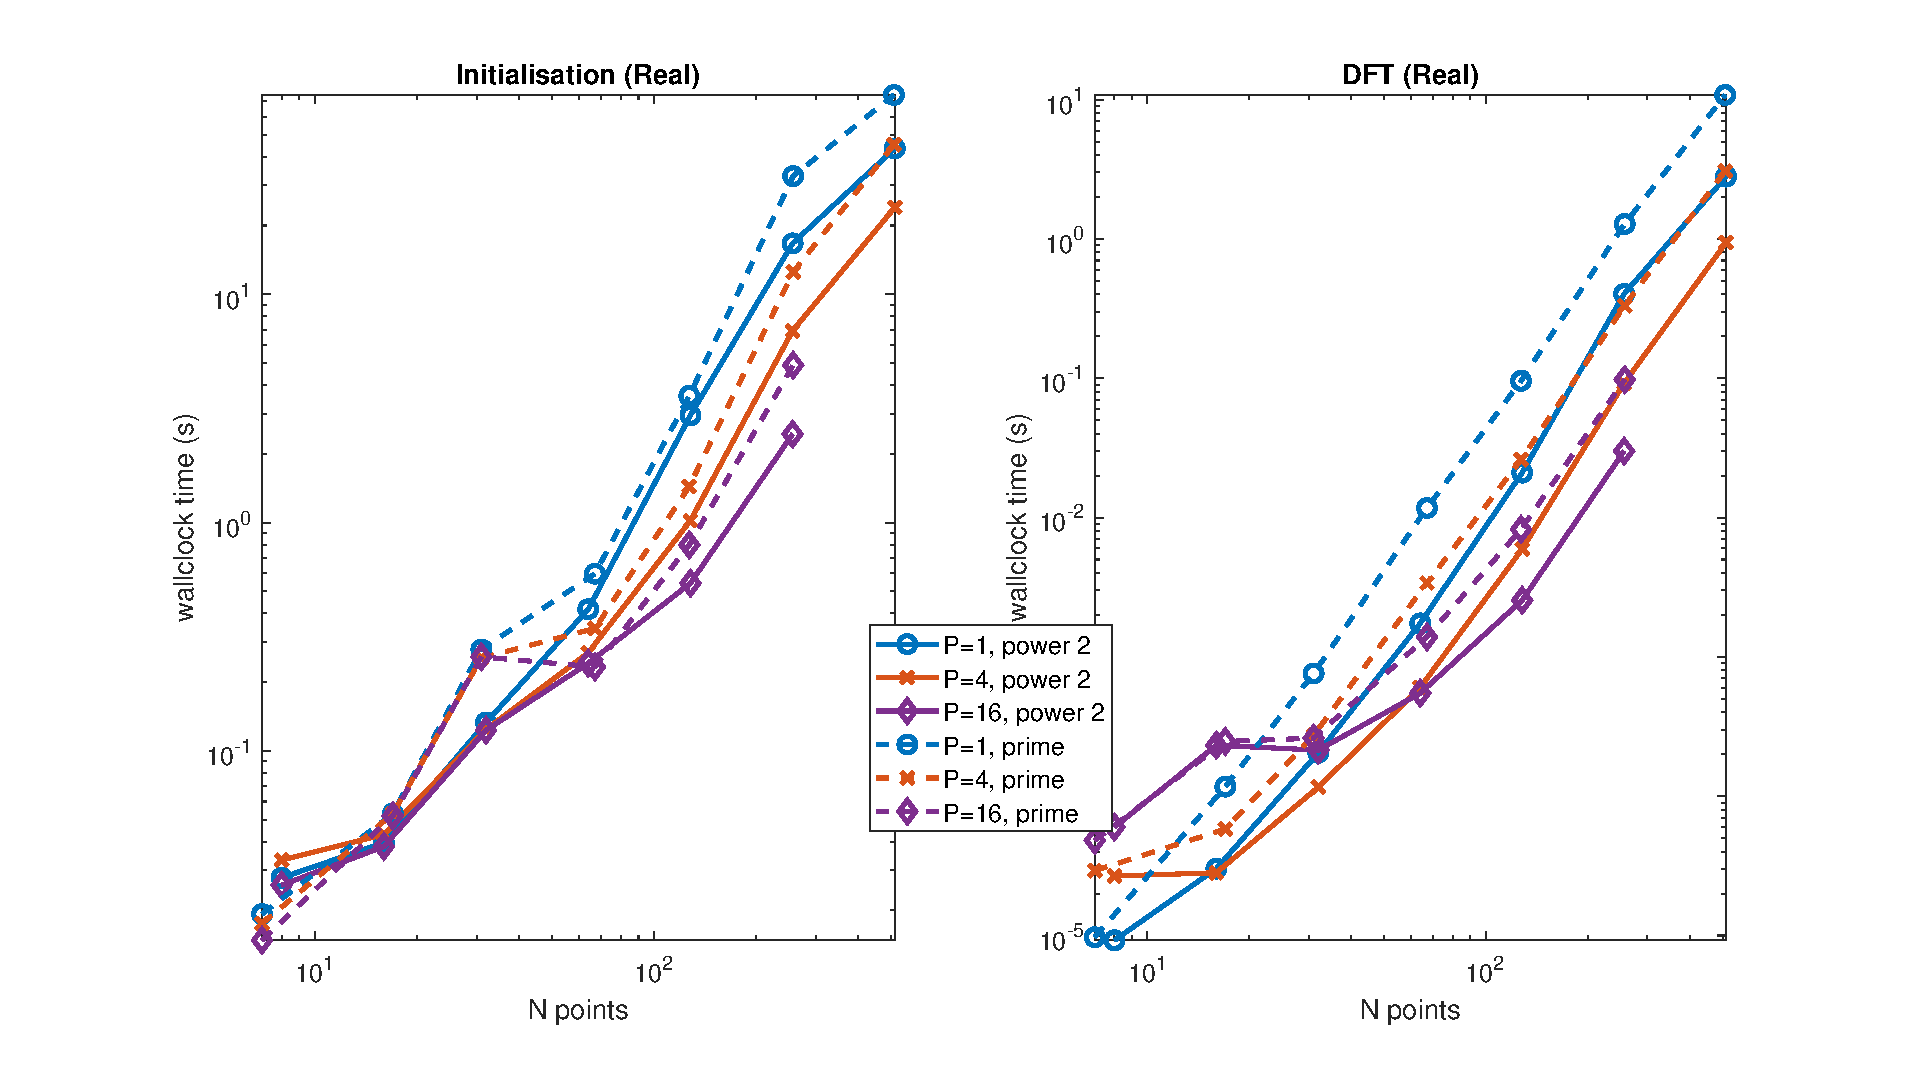
\includegraphics[width=0.9\linewidth]{../results/p3dfft_3d_mpi.eps}
  \caption{Initialisation and DFT execution times of distributed P3DFFT library applied to 3D signal as a function of the
    number of points, $N,$ and varying the number of MPI processes, $P,$ with one thread per process.}
  \label{3DDistP3DFFT}
\end{figure}

Comparing the DFT execution times in Figure~\ref{3DDistP3DFFT}, for
$N$ equal to 7 or 8, $P=1$ has the optimal time over those compared in
the figure. For $N=16,$ the DFT execution times are almost identical
for $P=1$ and $P=4$ but significantly larger for $P=16;$ for $N=17,$
$P=4$ has a lower DFT time than $P=1$ and $P=16$ is significantly
higher than both $P=1$ and 4. For $N>32,$ $P=16$ starts to outperform
the other values in the figure. Looking at the values of the DFT
execution times in Tables~\ref{Tbl:P3DFFT3d256} and
\ref{Tbl:P3DFFT3d257}, we observe that, with respect to $P,$ P3DFFT
has good strong scaling properties.

\begin{figure}[htb]
    \centering
    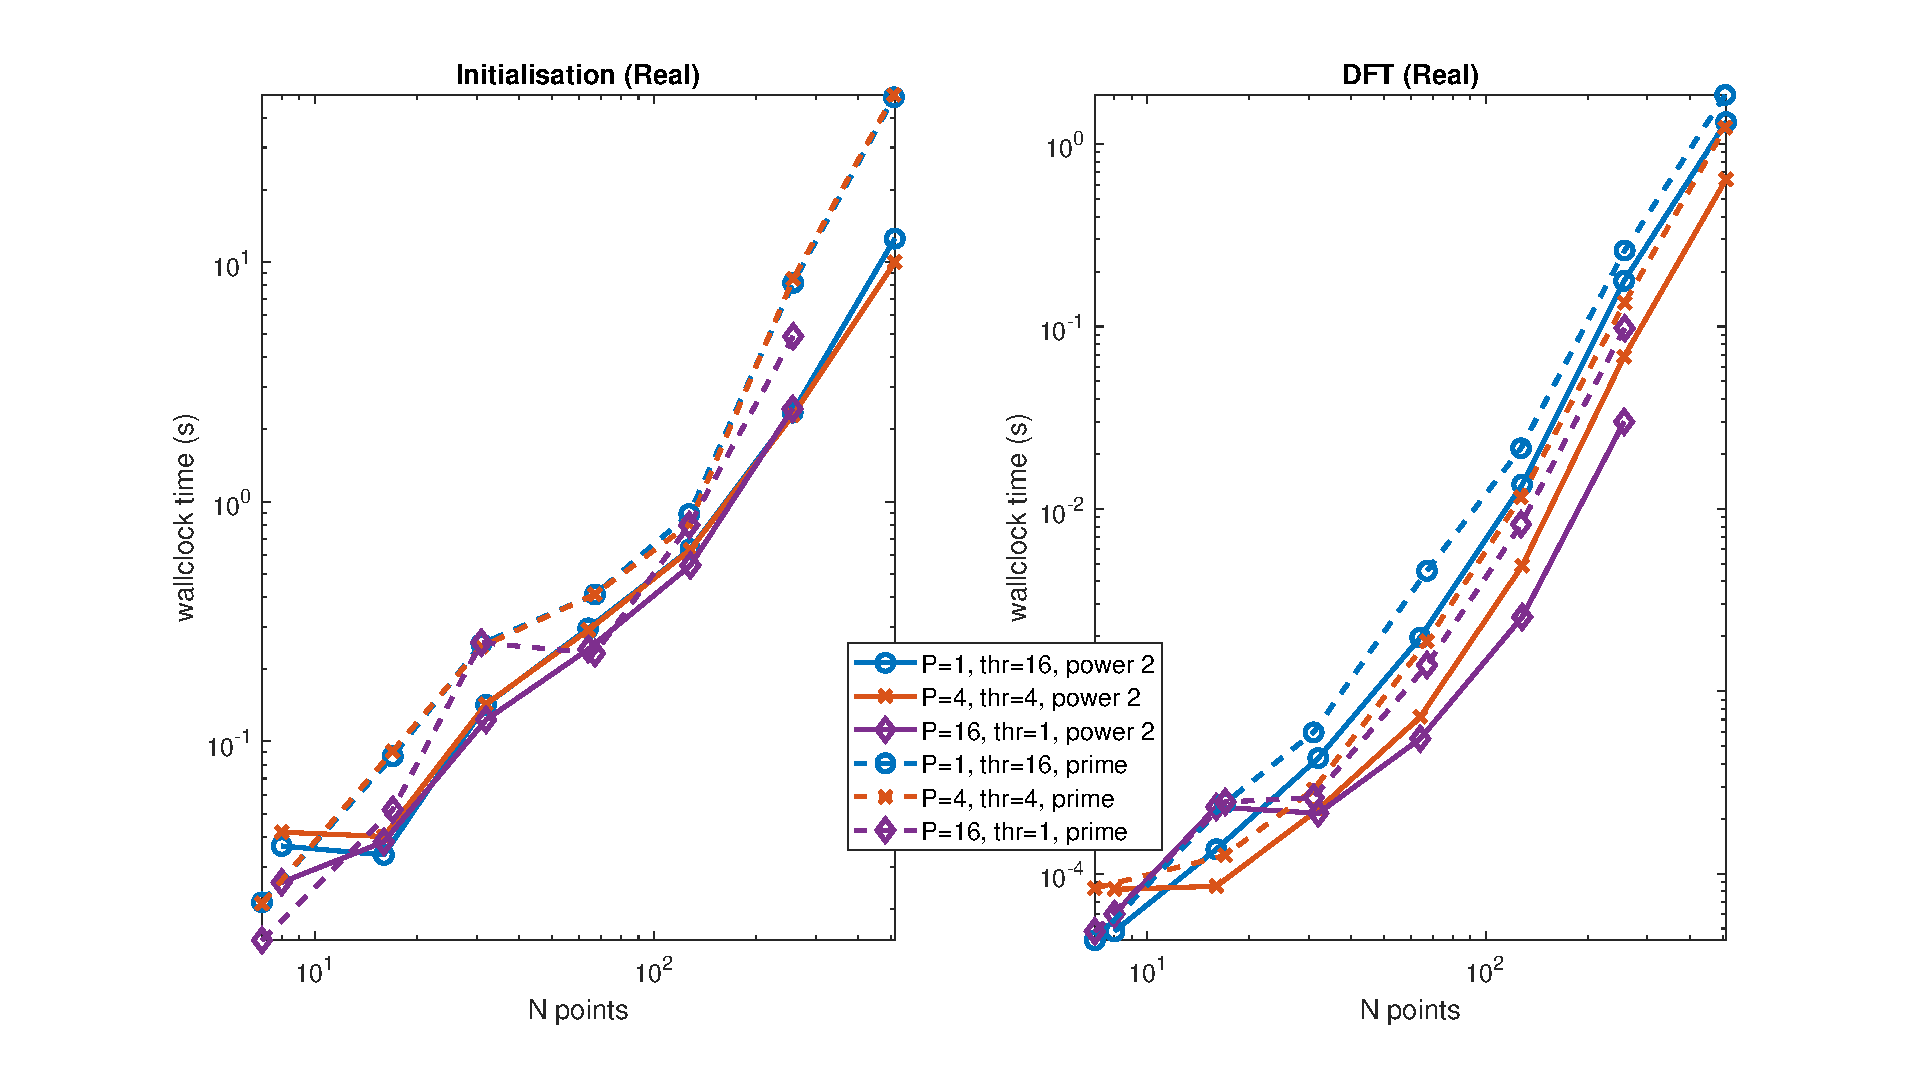
\includegraphics[width=0.9\linewidth]{../results/p3dfft_3d_mpi_thr.eps}
  \caption{Initialisation and DFT execution times of distributed P3DFFT library applied to 3D signal as a function of the
    number of points, $N,$ and varying the number of MPI processes, $P,$ and threads, $thr,$ whilst maintaining $P\times thr=16.$}
  \label{3DDistP3DFFT16}
\end{figure}

In Figure~\ref{3DDistP3DFFT16}, we compare P3DFFT's initialisation
times for $P\times thr=16,$ where $P=1,$ 4 and 16. For $N$ a power of
2, we see little difference in terms of initialisation times but when
$N$ is prime, $P=16$ with $thr=1$ is normally the optimal choice for
the values of $N$ considered. If we consider the DFT execution times,
then for $N>32,$ it is better increase the number of MPI processes and
reduce the number of OpenMP threads.

If we consider the benchmark data for $N=256$
(Tables~\ref{Tbl:P3DFFT3d256}), we see that the best initialisation
time was achieved with $P=2$ with $thr=12$ and the smallest average
DFT execution time occured when $P=24$ with $thr=1.$ As in previous
sections, if we consider the (average) time to perform a single
initialisation followed by $k$ DFT calculations, then $P=24$ with
$thr=1$ will outperform $P=2$ with $thr=12$ for all $k>3.$ When
$N=257,$ $P=16$ with $thr=1$ gives the lowest initialisation and DFT
execution times.





\subsection{Comparison of distributed libraries for 3D benchmark}\label{Sec:3DDistComp}

For $N$ a multiple of 2 and $N$ prime, we compare the FFTW, MKL and
P3DFFT libraries in Figures~\ref{3DDistFFTWMKLP3DFFT2} and
\ref{3DDistFFTWMKLP3DFFTprime}, respectively, for $P=1,$ 4 and 16 MPI
processes and $thr=1$ OpenMP threads. In terms of initialisation
times, in all but the smallest values of $N$ considered, MKL has the
best initialisation times and, in the real case, P3DFFT has the worst
(in general). In Table~\ref{Tbl:3DCompP}, we provide the
initialisation and DFT execution times for the three libraries,
$N=256$ and 257, for $P=1,$ 4 and 16 (8 instead of 16 in the case of
FFTW for $N=257$) with a single thread per process. We observe the
stark differences in initialisation times with MKL having times
several orders of magnitude smaller than FFTW and P3DFFT.



\begin{figure}[htb]
    \centering
    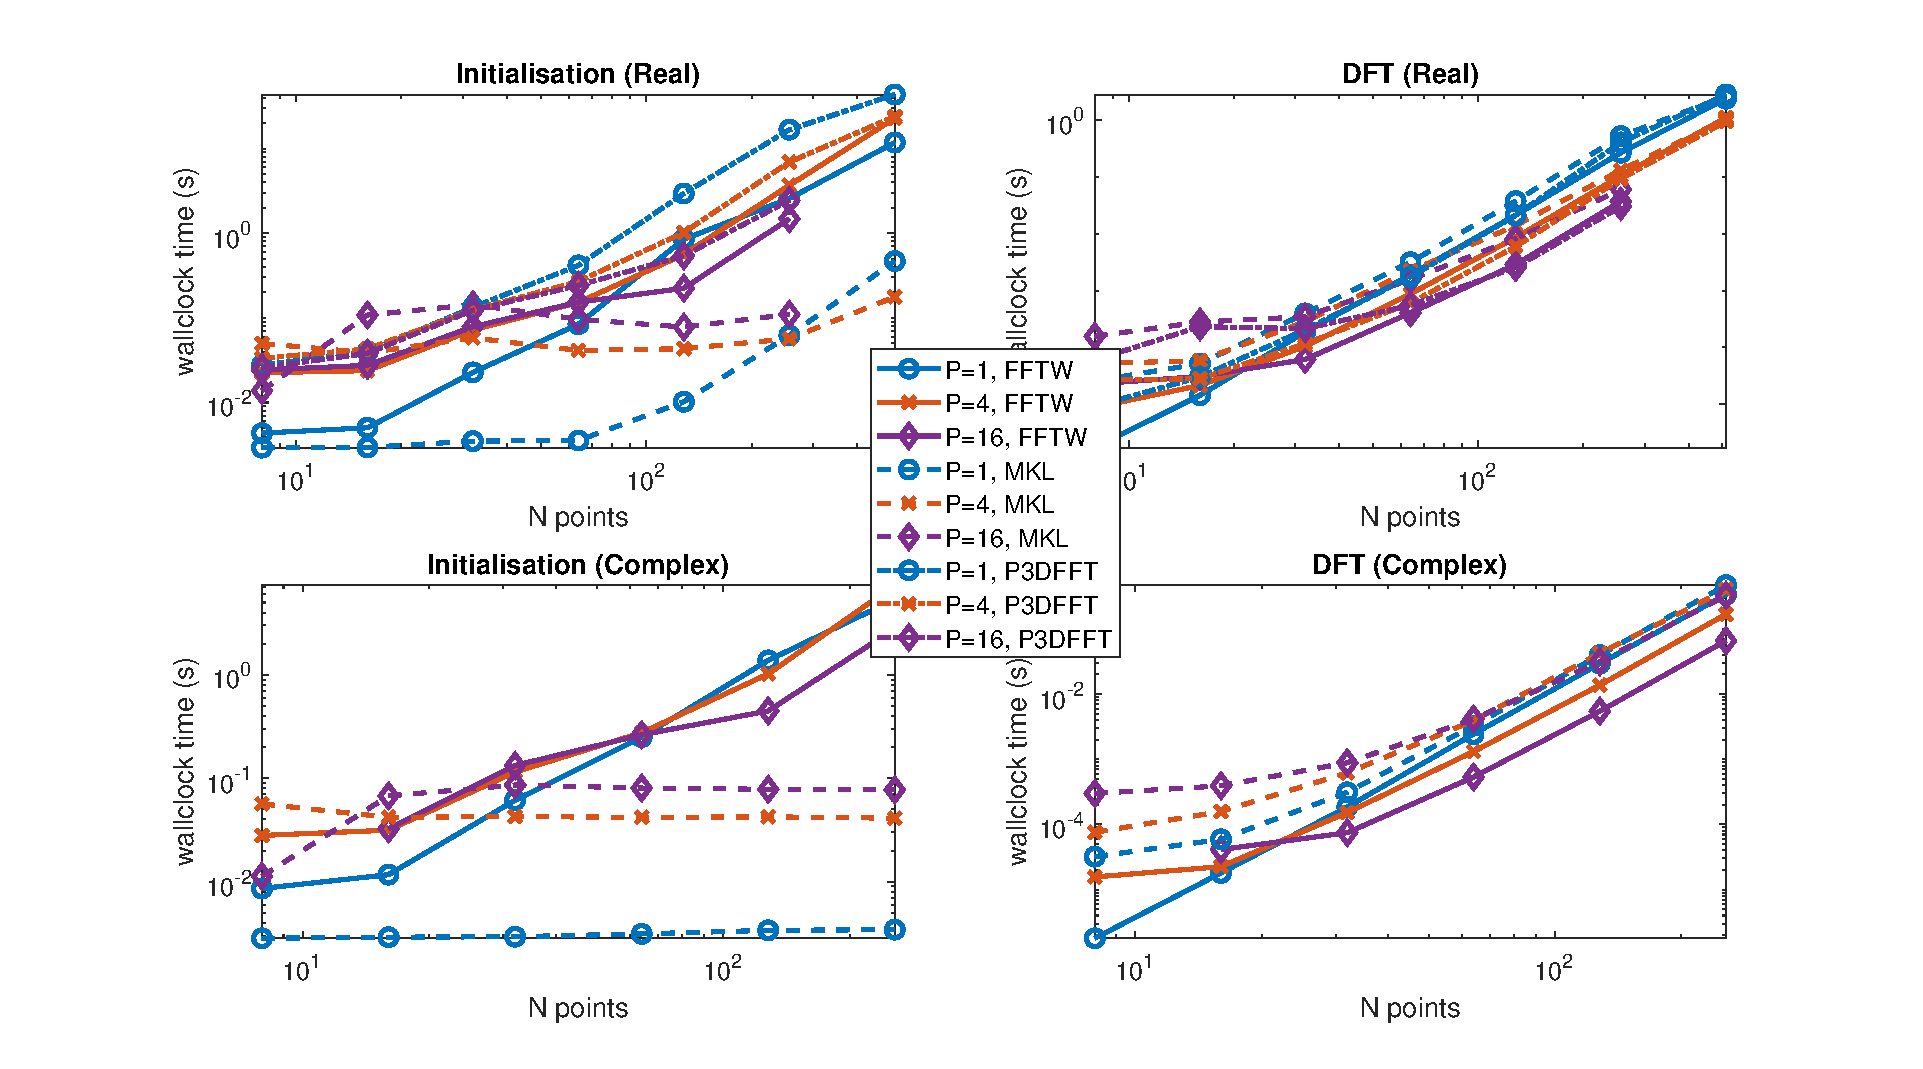
\includegraphics[width=0.9\linewidth]{../results/fftw_mkl_p3dfft_2_3d_mpi.eps}
  \caption{Initialisation and DFT execution times of distributed FFTW, MKL and P3DFFT libraries applied to 3D signal as a function of the
    number of points, $N,$ and varying the number of MPI processes, $P,$ with one thread per process. $N$ is a power of 2.}
  \label{3DDistFFTWMKLP3DFFT2}
\end{figure}


\begin{figure}[htb]
    \centering
    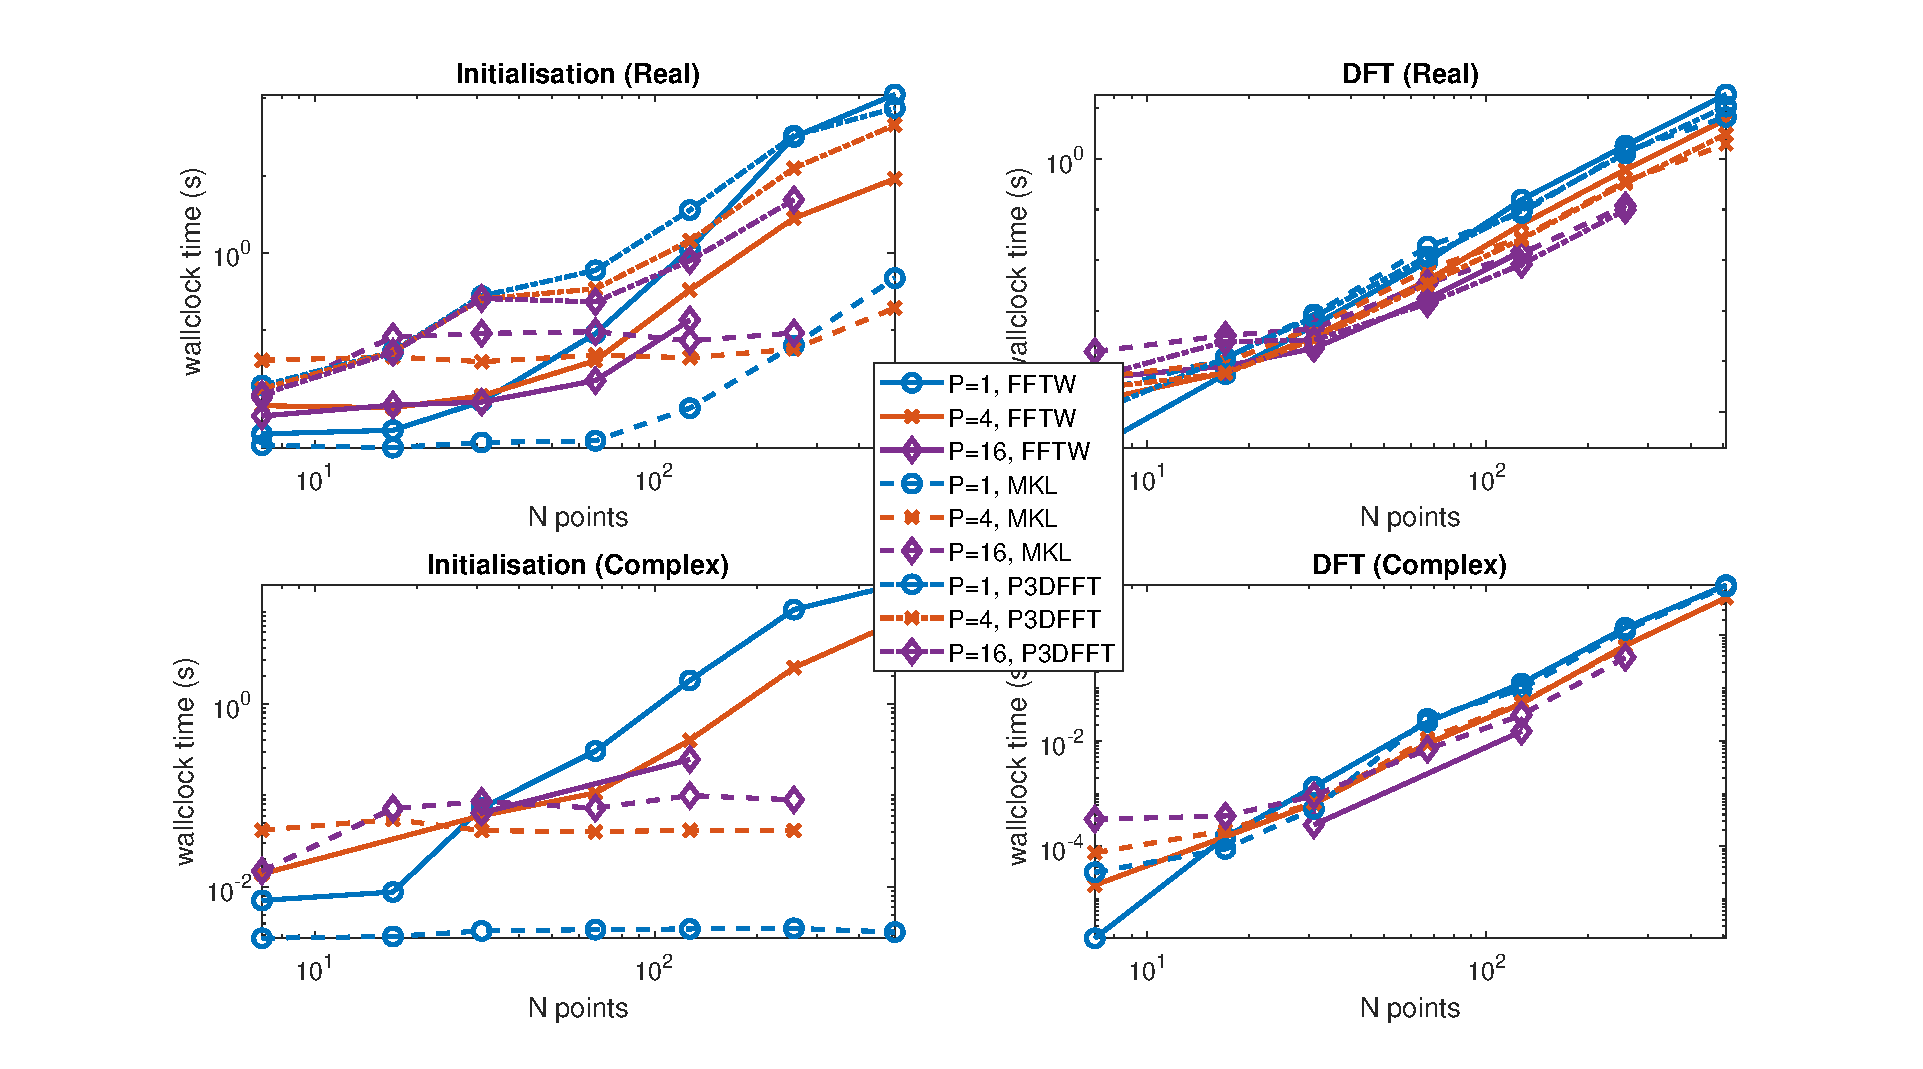
\includegraphics[width=0.9\linewidth]{../results/fftw_mkl_p3dfft_prime_3d_mpi.eps}
  \caption{Initialisation and DFT execution times of distributed FFTW, MKL and P3DFFT libraries applied to 3D signal as a function of the
    number of points, $N,$ and varying the number of MPI processes, $P,$ with one thread per process. $N$ is a prime number.}
  \label{3DDistFFTWMKLP3DFFTprime}
\end{figure}


\begin{table}[!htbp]
\begin{center}
%\being{small}
\begin{tabular}{|r|r|r|r|r|r||r|r|r|r|r|r|}\hline
R/C & $N$ & $P$ & Library & Init & DFT & R/C & $N$ & $P$ & Library & Init & DFT\\ \hline
 R & 256 & 1 & FFTW &   2.57   &  2.65e-1  & C & 256 & 1 & FFTW &  5.36   &  3.37e-1  \\
  &  &  & MKL &   6.22e-2   &   5.20e-1  &   &  &  & MKL &   3.44e-3   &  4.69e-1   \\
  &  &  & P3DFFT &  1.67e+1   &   4.03e-1  &   &  &  & P3DFFT &  -   &  -  \\ \hline
 R & 256 & 4 & FFTW &   3.68    &   1.04e-1  &  C & 256 & 4 & FFTW &   7.36   &  1.68e-1  \\
  &  &  & MKL &  5.68e-2   &   1.31e-1  &  &  &  & MKL &   4.11e-2   &   3.99e-1  \\
  &  &  & P3DFFT &  6.92   &   9.21e-2 &  &  &  & P3DFFT &  -   &  -  \\ \hline
 R & 256 & 16 & FFTW &  1.48   &  3.70e-2  & C & 256 & 16 & FFTW &  2.80   &  6.58e-2  \\
  &  &  & MKL &   1.10e-1   &    5.99e-2 &  &  &  & MKL &   7.73e-2   &   3.26e-1  \\
  &  &  & P3DFFT &  2.44   &  3.00e-2  &  &  &  & P3DFFT &  -   &  -  \\ \hline\hline
 R & 257 & 1 & FFTW &  3.16e+1   &  1.83  & C & 257 & 1 & FFTW &   1.06e+1   &  1.40   \\
  &  &  & MKL &   6.38e-2   &   1.42  &  &  &  & MKL &   3.54e-3   &   1.24  \\
  &  &  & P3DFFT & 3.29e+1    &   1.28  &  &  &  & P3DFFT &  -   & -   \\ \hline
 R & 257 & 4 & FFTW &   2.82    &   6.10e-1  & C & 257 & 4 & FFTW &  2.46   &  6.46e-1  \\
  &  &  & MKL &   5.72e-2   &   3.61e-1  &  &  &  & MKL &  4.12e-2    &   5.97e-1  \\
  &  &  & P3DFFT &   1.25e+1   &  3.32e-1 &  &  &  & P3DFFT &  -   &  -  \\ \hline
 R & 257 & 8 & FFTW &  1.61   &  3.35e-1  & C & 257 & 8 & FFTW &  2.06   &   3.50e-1  \\
  &  & 16 & MKL &    9.23e-2  &  1.19e-1  &  &  & 16 & MKL &   8.93e-2   &  3.83e-1   \\
  &  & 16 & P3DFFT &   4.89   &   9.77e-2  &  &  & 16 & P3DFFT &  -   &  -  \\ \hline\hline
\end{tabular}
\caption{ Initialisation (Init) and DFT execution times (DFT) for FFTW, MKL and P3DFFT with $N=256$ and 257, $thr=1,$ real (R) or complex (C) input signals for different numbers of MPI processes, $P.$ }\label{Tbl:3DCompP}
%\end{small}
\end{center}
\end{table}


 Comparing DFT execution times in Figures~\ref{3DDistFFTWMKLP3DFFT2}
 and \ref{3DDistFFTWMKLP3DFFTprime}, there does not appear to be such
 a marked difference between the libraries for the larger values of
 $N.$ This is confirmed in Table~\ref{Tbl:3DCompP}, where we see that
 for $N=256$ the FFTW library outperforms the MKL library but, in the
 real case, only outperforms P3DFFT in our table when $P=1:$ looking
 at the DFT times for $thr=1$ in Tables~\ref{Tbl:FFTW3d256} and
 \ref{Tbl:P3DFFT3d256}, we see that this holds for all of the values
 of $P>1$ considered. For $N=257,$ P3DFFT outperforms both FFTW and
 MKL in the real case in the benchmarks provided in
 Table~\ref{Tbl:3DCompP} and MKL outperforms FFTW; in the complex
 case, MKL outperforms FFTW for $P=1$ and 4 and, using
 Tables~\ref{Tbl:FFTW3d257} and \ref{Tbl:P3DFFT3d257}, we observe that
 FFTW only outperforms MKL when $P=1.$

 In each of the previous sections, we identified the combinations of
 $P$ and $thr$ that gave optimal initialisation and DFT execution
 times for $N=256$ and $N=257$ with real and complex input
 signals. For these combinations, we can compare the (average) time to
 perform a single initialisation and $k$ DFT calculations across the
 libraries, see Table~\ref{Tbl:3DCompk}. We can see that in the real
 case, P3DFFT using 24 MPI processes on the node with a single thread
 per process out performs the other libraries for large enough values
 of $k$ and, for the smaller values of $k$ that are greater than 1,
 MKL is the optimal library with $P=16$ and $thr=1.$ In the complex
 case, for larger values of $k$ it is better to use FFTW with a single
 MPI process and a large number of threads; for small values of $k,$
 we would recommend using the MKL with a single MPI process and large
 number of threads. 

 \begin{table}[!htbp]
\begin{center}
%\being{small}
\begin{tabular}{|r|r|r|r|r|r||r|r|r|r|r|r|}\hline
R/C & $N$ & $k$ & Optimal Library \\ \hline
R & 256 & 1 & MKL($P=4,$ $thr=4$) \\
  &     & $[2,58]$ & MKL($P=16,$ $thr=1$) \\
  &     & $[59,\infty)$ & P3DFFT($P=24,$ $thr=1$) \\\hline
C & 256 & $[1,20]$ & MKL($P=1,$ $thr=24$) \\
  &     & $[21,182]$ & FFTW($P=16,$ $thr=1$) \\
  &     & $[183,\infty)$ & FFTW($P=1,$ $thr=16$) \\\hline
R & 257 & 1 & MKL($P=4,$ $thr=4$) \\
  &     & $[2,223]$ & MKL($P=16,$ $thr=1$) \\
  &     & $[224,\infty)$ & P3DFFT($P=16,$ $thr=1$) \\\hline
C & 257 & $[1,113]$ & MKL($P=1,$ $thr=16$) \\
  &     & $[114,\infty)$ & FFTW($P=1,$ $thr=24$) \\\hline
\end{tabular}
\caption{ Library that gives optimal time to perform a single initialisation and $k$ DFT calculations. For the comparison, for each library we used the set of values of $P$ and $thr$ that gave either the optimal initialisation time or the optimal DFT execution time.  }\label{Tbl:3DCompk}
%\end{small}
\end{center}
\end{table}

 

\section{Conclusions}\label{Sec:Conclusions}

We planned to benchmark four FFT libraries that have interfaces for
Fortran: FFTE, FFTW, MKL and P3DFFT. Unfortunately, FFTE was found to
be undocumented and when we tested it, we discovered that the OpenMP
version was unreliable and the MPI version had restrictions on the
number of MPI processes that can be used but the library does not
return error states so the user is unaware that the returned answer is
not correct. Hence, we excluded FFTE from our benchmarks.

All of the three remaining libraries were found to have limitations:
\begin{itemize}
\item FFTW is written in C and a Fortran interface has been created
  that uses C\_INTPTR\_T, which, on ARCHER, has size 4 bytes. In the
  Fortran interface, the dimensions of the arrays that are being
  operated on are type C\_INTPTR\_T, so the size of problem is
  restricted to all dimensions being at most 4 bytes in size. The
  distributed version of the FFTW library for 1D input signals only
  has an interface for complex arrays.
 \item The distributed version of the MKL library has restrictions on
   the lengths of transforms. For the 1D interface, the length must be the
   product of two integers and each of these integers must not be less
   than the number of MPI processes, which means that the transform
   length cannot be prime if multiple MPI processes are being
   used. For multi-dimensional transforms, the lengths of the last two
   dimensions must not be less than the number of processes.
 \item P3DFFT only allows real 3D input signals and, due to the nature
   of its underlying data structures, we cannot set the redundant
   dimensions to 1 to compute a 1D or 2D transform.

\end{itemize}
Hence, if one of the dimensions exceeds the range of values that
C\_INTPTR\_T can store, FFTW will not be suitable for use on ARCHER or
other systems where C\_INTPTR\_T has size 4 bytes. If you want to
perform the FFT of a 1D signal that has length that is prime and wish
to use multiple MPI processes, then this is not possible to do with
either the MKL library or the P3DFFT library. There is, therefore, no
single library (from thos considered) that will work in every
situation and care must be taken to ensure that the library chosen
will satisfy all of the scenarios that will reastically occur.

In our multithreading investigations, we revealed that MKL is
generally performing better than FFTW and, in the 3D case, also
outperforming P3DFFT. For larger problems, the use of multiple threads
was advantageous across all of the libraries.

The three libraries considered all have distributed versions of the
library that have MPI and OpenMP capabilities. For 1D problems, when
the MKL library can be used, it outperforms FFTW. In both cases,
increasing the number of MPI processes was advantageous for the larger
problem size. For 2D and 3D problems, it was advantageous to use
larger numbers of MPI process for larger problems sizes but the choice
of favourable library will depend on the properties of the underlying
problems and how many DFTS are being performed per initialisation.





\section*{Acknowledgements}
This work made use of computational support by CoSeC, the
Computational Science Centre for Research Communities, through its
Software Outlook activity.

\bibliographystyle{siam}
\bibliography{bib2017}

\clearpage

\appendix

\section{1D Multithreaded Data}\label{App:1Dthr}


\begin{table}[!htbp]
\begin{center}
\begin{small}
\begin{tabular}{|r|r|r|r|r|r|r|r|r|r|}
\hline 
     \multicolumn{3}{|c|}{ } & \multicolumn{7}{c|}{$thr$} \\ \hline
    $N$  & & R/C  & 1           & 2    & 4    & 8    & 12   & 16    & 24  \\ \hline\hline
    2048  & ftime & R  &  1.09e-5 &   1.71e-5 &   3.00e-5 &   3.49e-5 &   4.05e-5 &   4.54e-5 &   6.26e-5   \\ 
      & fratio & & 1.00 &    1.57 &    2.75 &    3.20 &    3.72 &    4.17 &    5.74   \\ 
     & itime & &  8.13e-2 &    1.09e-1 &   1.18e-1 &   1.42e-1 &   1.72e-1 &   1.62e-1 &   2.14e-1    \\ 
     & iratio & &   1.00 &    1.34 &    1.45 &    1.75 &    2.12 &    1.99 &    2.63    \\ \hline 
    2053  & ftime & R &  1.03e-4 &   1.20e-4 &   1.73e-4 &   1.93e-4 &   2.50e-4 &   3.81e-4 &   7.14e-4    \\ 
      & fratio & & 1.00 &   1.17 &   1.68 &   1.87 &   2.43 &   3.70 &   6.93    \\ 
     & itime &  &   1.08e0 &   1.71e0 &   2.07e0 &   2.51e0 &   2.93e0 &   3.21e0 &   3.79e0   \\ 
    & iratio &  &     1.00 &   1.58 &   1.92 &   2.32 &   2.71 &   2.97 &   3.51     \\ \hline 
  16381  & ftime & R &  7.97e-4 &   7.98e-4 &   8.19e-4 &   8.25e-4 &   8.30e-4 &   8.47e-4 &   9.57e-4     \\ 
      & fratio & &  1.00 &   1.00 &   1.03 &   1.04 &   1.04 &   1.06 &   1.20    \\ 
     & itime & &  1.51e0 &   2.05e0 &   2.29e0 &   2.56e0 &   2.84e0 &   3.07e0 &   3.67e0     \\ 
     & iratio & &  1.00 &   1.36 &   1.52 &   1.70 &   1.88 &   2.03 &   2.43     \\ \hline 
 16384  & ftime & R & 1.11e-4 &   8.58e-5 &   9.49e-5 &   8.59e-5 &   9.79e-5 &   2.06e-4 &   5.42e-4   \\ 
      & fratio & & 1.00 &   0.77 &   0.85 &   0.77 &   0.88 &   1.86 &   4.88  \\
     & itime & & 1.90e-1 &   2.62e-1 &   2.55e-1 &   2.60e-1 &   3.07e-1 &   2.90e-1 &   3.98e-1   \\ 
 & iratio & & 1.00 &   1.38 &   1.34 &   1.37 &   1.62 &   1.53 &   2.09   \\  \hline \hline
    2048  & ftime & C  &  1.01e-5 &   1.84e-5 &   2.98e-5 &   3.39e-5 &   3.72e-5 &   4.94e-5 &   5.92e-5   \\ 
      & fratio & &  1.00 &   1.82 &   2.95 &   3.36 &   3.68 &   4.89 &   5.86  \\ 
     & itime & &   1.07e-1 &   1.16e-1 &   1.55e-1 &   1.80e-1 &   2.10e-1 &   2.12e-1 &   2.68e-1   \\ 
     & iratio & &  1.00 &   1.08 &   1.45 &   1.68 &   1.96 &   1.98 &   2.50     \\ \hline 
    2053  & ftime & C &  7.76e-5 &   1.03e-4 &   1.32e-4 &   1.81e-4 &   1.83e-4 &   2.30e-4 &   4.48e-4     \\ 
      & fratio & &  1.00 &   1.33 &   1.70 &   2.33 &   2.36 &   2.96 &   5.77   \\ 
     & itime &  &  1.03e0 &   1.06e0 &   1.24e0 &   1.47e0 &   1.74e0 &   1.89e0 &   2.21e0    \\ 
    & iratio &  &  1.00 &   1.03 &   1.20 &   1.43 &   1.69 &   1.84 &   2.15       \\ \hline
  16381  & ftime & C &   1.03e-3 &   6.76e-4 &   6.62e-4 &   6.40e-4 &   6.74e-4 &   6.07e-4 &   7.91e-4     \\ 
      & fratio & &  1.00 &   0.66 &  0.64 &   0.62 &  0.65 &   0.59 &  0.77   \\ 
     & itime & &   1.72e0 &   1.64e0 &   1.52e0 &   1.58e0 &   1.51e0 &   1.38e0 &   1.78e0    \\ 
     & iratio & &   1.00 &   0.95 &  0.88 &  0.92 &  0.88 &  0.80 &  1.03    \\ \hline
 16384  & ftime & C &  1.21e-4 &   8.86e-5 &   1.09e-4 &   8.21e-5 &   8.88e-5 &   7.61e-5 &   2.39e-4  \\ 
      & fratio & & 1.00 &   0.73 &  0.90 &  0.68 &  0.73 &  0.63 &  1.98  \\
     & itime & &  5.30e-1 &   5.01e-1 &   5.07e-1 &   5.22e-1 &   5.37e-1 &   5.53e-1 &   6.53e-1   \\ 
 & iratio & &  1.00 &   0.95 &  0.96 &  0.98 &  1.01 &   1.04 &   1.23  \\  \hline 
\end{tabular}
\caption{1D FFTW applied to real (R) and complex (C) valued one-dimensional arrays of length $N=2048,$ 2053, 16381, 16384, 1048573 and 1048576 using $thr$ threads. The wallclock DFT computation time, ftime, and wallclock DFT initialisation time, itime, both in seconds, are provided. Additionally,  the ratio, fratio, of ftime  with ftime($thr=1$) and the ratio, iratio, of itime  with itime($thr=1$) is provided. }\label{Tbl:FFTW1d}
\end{small}
\end{center}
\end{table}




\begin{table}[htbp]
\begin{center}
\begin{small}
\begin{tabular}{|r|r|r|r|r|r|r|r|r|r|}
\hline 
     \multicolumn{3}{|c|}{ } & \multicolumn{7}{c|}{$thr$} \\ \hline
    $N$  & & R/C  & 1           & 2    & 4    & 8    & 12   & 16    & 24  \\ \hline\hline
    2048  & ftime & R  &  6.21e-6 &   8.79e-6 &   6.05e-6 &   6.38e-6 &   7.32e-6 &   6.69e-6 &   7.08e-6  \\ 
      & fratio & & 1.00 &   1.42 &   0.97 &   1.03 &   1.13 &   1.03 &   1.14   \\ 
     & itime & &    2.82e-3 &   1.27e-2 &   1.83e-2 &   1.72e-2 &   1.75e-2 &   1.67e-2 &   1.66e-2   \\ 
     & iratio & &   1.00 &   4.50 &   6.49 &   6.10 &   6.21 &   5.92 &   5.89    \\ \hline 
    2053  & ftime & R &  7.74e-5 & 7.99e-5 &   7.77e-5 &   1.06e-4 &   8.25e-5 &   8.11e-5 &   8.33e-5    \\ 
      & fratio & &  1.00 &   1.03 &   1.00 &   1.37 &   1.07 &   1.05 &   1.08   \\ 
     & itime &  &   2.85e-3 &   1.26e-2 &   2.19e-2 &   2.59e-2 &   1.40e-2 &   1.75e-2 &   1.69e-2    \\ 
    & iratio &  &     1.00 &   4.42 &   7.68 &   9.09 &   4.91 &   6.14 &   5.93     \\ \hline 
  16381  & ftime & R &  6.68e-4 &   6.47e-4 &   6.73e-4 &   6.81e-4 &   6.68e-4 &   6.84e-4 &   7.32e-4      \\ 
      & fratio & &  1.00 &   0.97 &   1.01 &   1.02 &   1.00 &   1.02 &   1.10    \\ 
     & itime & &   4.14e-3 &   1.31e-2 &   1.91e-2 &   2.75e-2 &   1.92e-2 &   1.90e-2 &   2.29e-2    \\ 
     & iratio & &  1.00 &   3.16 &   4.61 &   6.64 &   4.64 &   4.59 &   5.53     \\ \hline 
 16384  & ftime & R &  6.30e-5 &   6.74e-5 &   6.98e-5 &   5.49e-5 &   6.03e-5 &   5.41e-5 &   6.23e-5   \\ 
      & fratio & &   1.00 &   1.07 &   1.11 &   0.87 &  0.96 &   0.86 &   0.99 \\
     & itime & &  2.80e-3 &   2.68e-3 &   1.53e-2 &   2.59e-2 &   1.70e-2 &   1.71e-2 &   1.60e-2   \\ 
 & iratio & &  1.00 &   0.96 &   5.46 &   9.25 &   6.07 &   6.11 &   5.71   \\  \hline 
  1048573  & ftime & R &    7.78e-2 &   7.74e-2 &   7.84e-2 &   7.97e-2 &   8.04e-2 &   8.03e-2 &   8.02e-2    \\ 
      & fratio & &  1.00 &   0.99 &   1.01 &   1.02 &   1.03 &   1.03 &   1.03    \\ 
     & itime & &   1.46e-1 &   1.48e-1 &   1.54e-1 &   1.57e-1 &   1.49e-1 &   1.51e-1 &   1.58e-1    \\ 
     & iratio & &   1.00 &   1.01 &   1.05 &   1.08 &   1.02 &   1.03 &   1.08    \\ \hline 
 1048576  & ftime & R &  6.71e-3 &   6.21e-3 &   3.59e-3 &   2.17e-3 &   2.31e-3 &   1.55e-3 &   1.78e-3   \\ 
      & fratio & & 1.00 &   0.93 &   0.54 &   0.32 &   0.34 &   0.23 &   0.27  \\
     & itime & & 1.01e-2 &   1.79e-2 &   1.11e-2 &   1.20e-2 &   6.88e-3 &   1.53e-2 &   1.81e-2    \\ 
 & iratio & &  1.00 &   1.77 &   1.10 &   1.19 &   0.68 &   1.51 &   1.79   \\  \hline \hline
    2048  & ftime & C  &  1.17e-5 &   1.99e-5 &   2.76e-5 &   3.92e-5 &   3.78e-5 &   4.06e-5 &   3.64e-5   \\ 
      & fratio & &  1.00 &   1.70 &   2.36 &   3.35 &   3.23 &   3.47 &   3.11   \\ 
     & itime & &  2.99e-3 &   1.26e-2 &   1.83e-2 &   1.86e-2 &   1.76e-2 &   1.75e-2 &   1.63e-2   \\ 
     & iratio & &  1.00 &   4.21 &   6.12 &   6.22 &   5.89 &   5.85 &   5.45    \\ \hline 
    2053  & ftime & C &  7.81e-5 &   7.73e-5 &   7.77e-5 &   7.87e-5 &   7.92e-5 &   7.76e-5 &   8.06e-5     \\ 
      & fratio & & 1.00 &   0.99 &   0.99 &   1.01 &   1.01 &   0.99 &   1.03    \\ 
     & itime &  & 3.33e-3 &   1.32e-2 &   1.87e-2 &   2.25e-2 &   2.21e-2 &   1.78e-2 &   1.74e-2    \\ 
    & iratio &  &    1.00 &   3.96 &   5.62 &   6.76 &   6.64 &   5.35 &   5.23     \\ \hline
  16381  & ftime & C &    6.42e-4 &   6.65e-4 &   6.66e-4 &   6.77e-4 &   6.67e-4 &   6.74e-4 &   7.02e-4     \\ 
      & fratio & & 1.00 &   1.04 &   1.04 &   1.05 &   1.04 &   1.05 &   1.09    \\ 
     & itime & &    5.33e-3 &   1.29e-2 &   1.74e-2 &   2.69e-2 &   2.32e-2 &   1.91e-2 &   1.91e-2    \\ 
     & iratio & &    1.00 &   2.42 &   3.26 &   5.05 &   4.35 &   3.58 &   3.58  \\ \hline
 16384  & ftime & C &  1.23e-4 &   1.15e-4 &   1.49e-4 &   1.39e-4 &   1.38e-4 &   1.45e-4 &   1.17e-4   \\ 
      & fratio & & 1.00 &   0.93 &   1.21 &   1.13 &   1.12 &   1.18 &   0.95  \\
     & itime & &  3.29e-3 &   1.07e-2 &   1.96e-2 &   1.70e-2 &   1.68e-2 &   1.69e-2 &   1.59e-2   \\ 
 & iratio & & 1.00 &   3.25 &   5.96 &   5.17 &   5.11 &   5.14 &   4.83   \\  \hline 
  1048573  & ftime & C &  7.80e-2 &   7.78e-2 &   7.88e-2 &   8.01e-2 &   8.06e-2 &   8.13e-2 &   8.25e-2      \\ 
      & fratio & &  1.00 &   1.00 &   1.01 &   1.03 &   1.03 &   1.04 &   1.06    \\ 
     & itime & &   1.46e-1 &   1.49e-1 &   1.52e-1 &   1.60e-1 &   1.50e-1 &   1.47e-1 &   1.59e-1   \\ 
     & iratio & &    1.00 &   1.02 &   1.04 &   1.10 &   1.03 &   1.01 &   1.09    \\ \hline 
 1048576  & ftime & C &  1.35e-2 &   1.37e-2 &   7.80e-3 &   5.64e-3 &   5.54e-3 &   6.83e-3 &   7.87e-3   \\ 
      & fratio & &  1.00 &   1.01 &   0.58 &   0.42 &   0.41 &   0.51 &   0.58  \\
     & itime & &  1.28e-2 &   3.83e-3 &   3.80e-3 &   1.52e-2 &   1.49e-2 &   4.15e-3 &   1.69e-2   \\ 
 & iratio & &  1.00 &   0.30 &   0.30 &   1.19 &   1.16 &   0.32 &   1.32 
  \\  \hline 
\end{tabular}
\caption{1D MKL applied to real (R) and complex (C) valued one-dimensional arrays of length $N=2048,$ 2053, 16381, 16384, 1048573 and 1048576  using $thr$ threads. The wallclock DFT computation time, ftime, and wallclock DFT initialisation time, itime, both in seconds, are provided. Additionally,  the ratio, fratio, of ftime  with ftime($thr=1$) and the ratio, iratio, of itime  with itime($thr=1$) is provided. }\label{Tbl:MKL1d}
\end{small}
\end{center}
\end{table}

\clearpage

\section{2D Multithreaded Data}\label{App:2Dthr}


\begin{table}[!htbp]
\begin{center}
\begin{small}
\begin{tabular}{|r|r|r|r|r|r|r|r|r|r|}
\hline 
     \multicolumn{3}{|c|}{ } & \multicolumn{7}{c|}{$thr$} \\ \hline
    $N$  & & R/C  & 1           & 2    & 4    & 8    & 12   & 16    & 24  \\ \hline\hline
    31  & ftime & R  &  1.26e-5 &   3.50e-5 &   2.81e-5 &   3.39e-5 &   6.63e-5 &   5.16e-5 &   7.92e-5   \\ 
      & fratio & &      1.00 &   2.78 &   2.23 &   2.69 &   5.26 &   4.10 &   6.29     \\ 
     & itime & &        2.59e-3 &   8.92e-3 &   8.00e-3 &   9.38e-3 &   1.55e-2 &   9.68e-3 &   1.39e-2     \\ 
     & iratio & &       1.00 &   3.44 &   3.09 &   3.62 &   5.98 &   3.74 &   5.37      \\ \hline 
    32  & ftime & R  &  3.05e-6 &   2.28e-5 &   2.34e-5 &   3.47e-5 &   5.42e-5 &   5.36e-5 &   8.02e-5   \\ 
      & fratio & &      1.00 &   7.48 &   7.67 &   11.4 &   17.8 &   17.6 &   26.3     \\ 
     & itime & &        1.11e-2 &   1.51e-2 &   1.46e-2 &   1.80e-2 &   4.30e-2 &   2.08e-2 &   2.55e-2     \\ 
     & iratio & &       1.00 &   1.36 &   1.32 &   1.62 &   3.87 &   1.87 &   2.30      \\ \hline 
   256  & ftime & R  &  5.38e-4 &   3.57e-4 &   2.63e-4 &   2.23e-4 &   2.08e-4 &   2.09e-4 &   2.36e-4   \\ 
      & fratio & &      1.00 &   0.66 &   0.49 &   0.41 &   0.39 &   0.39 &   0.44     \\ 
     & itime & &        6.39e-2 &   7.77e-2 &   7.55e-2 &   8.82e-2 &   1.09e-1 &   9.52e-2 &   1.38e-1     \\ 
     & iratio & &       1.00 &   1.22 &   1.18 &   1.38 &   1.71 &   1.49 &   2.16      \\ \hline 
   257  & ftime & R  &  4.55e-3 &   2.56e-3 &   1.67e-3 &   1.26e-3 &   7.97e-4 &   8.17e-4 &   8.08e-4   \\ 
      & fratio & &      1.00 &   0.56 &   0.37 &   0.28 &   0.18 &   0.18 &   0.18     \\ 
     & itime & &        1.44e-1 &   2.47e-1 &   3.43e-1 &   3.81e-1 &   4.80e-1 &   4.92e-1 &   6.23e-1     \\ 
     & iratio & &       1.00 &   1.72 &   2.38 &   2.65 &   3.33 &   3.42 &   4.33      \\ \hline 
  2048  & ftime & R  &  5.71e-2 &   3.30e-2 &   2.09e-2 &   1.04e-2 &   1.22e-2 &   1.10e-2 &   1.04e-2   \\ 
      & fratio & &      1.00 &   0.58 &   0.37 &   0.18 &   0.21 &   0.19 &   0.18     \\ 
     & itime & &        8.09e-1 &   1.31e0 &   1.06e0 &   1.02e0 &   1.42e0 &   1.13e0 &   1.28e0     \\ 
     & iratio & &       1.00 &   1.62 &   1.31 &   1.26 &   1.76 &   1.40 &   1.58      \\ \hline 
  2053  & ftime & R  &  4.05e-1 &   2.44e-1 &   1.39e-1 &   8.00e-2 &   5.74e-2 &   4.66e-2 &   3.28e-2   \\ 
      & fratio & &      1.00 &   0.60 &   0.34 &   0.20 &   0.14 &   0.12 &   0.08    \\ 
     & itime & &        6.62e0 &   7.76e0 &   5.77e0 &   4.95e0 &   4.03e0 &   4.61e0 &   4.96e0     \\ 
     & iratio & &       1.00 &   1.17 &   0.87 &   0.75 &   0.61 &   0.70 &   0.75      \\ \hline 
\end{tabular}
\caption{2D FFTW applied to real (R)  valued two-dimensional square arrays with length $N=31,$ 32, 256, 257, 2048 and 2053 along each side and using $thr$ threads. The wallclock DFT computation time, ftime, and wallclock DFT initialisation time, itime, both in seconds, are provided. Additionally,  the ratio, fratio, of ftime  with ftime($thr=1$) and the ratio, iratio, of itime  with itime($thr=1$) is provided. }\label{Tbl:FFTW2d}
\end{small}
\end{center}
\end{table}




\begin{table}[htbp]
\begin{center}
\begin{small}
\begin{tabular}{|r|r|r|r|r|r|r|r|r|r|}
\hline 
     \multicolumn{3}{|c|}{ } & \multicolumn{7}{c|}{$thr$} \\ \hline
    $N$  & & R/C  & 1           & 2    & 4    & 8    & 12   & 16    & 24  \\ \hline\hline
    31  & ftime & C  &  2.86e-5 &   2.89e-5 &   3.37e-5 &   4.04e-5 &   6.06e-5 &   7.31e-5 &   1.10e-4   \\ 
      & fratio & &      1.00 &   1.01 &   1.18 &   1.41 &   2.12 &   2.56 &   3.85     \\ 
     & itime & &        4.60e-2 &   5.31e-2 &   5.12e-2 &   8.48e-2 &   9.37e-2 &   1.29e-1 &   1.61e-1     \\ 
     & iratio & &       1.00 &   1.15 &   1.11 &   1.84 &   2.04 &   2.80 &   3.50      \\ \hline 
    32  & ftime & C  &  2.91e-6 &   1.33e-5 &   2.37e-5 &   3.49e-5 &   6.83e-5 &   5.98e-5 &   8.59e-5   \\ 
      & fratio & &      1.00 &   4.57 &   8.14 &   12.0 &   23.5 &   20.6 &   29.5     \\ 
     & itime & &        3.18e-2 &   3.82e-2 &   3.73e-2 &   3.80e-2 &   5.56e-2 &   4.73e-2 &   5.17e-2     \\ 
     & iratio & &       1.00 &   1.20 &   1.17 &   1.20 &   1.75 &   1.49 &   1.63      \\ \hline 
   256  & ftime & C  &  5.46e-4 &   3.52e-4 &   3.79e-4 &   3.39e-4 &   2.56e-4 &   2.31e-4 &   3.10e-4   \\ 
      & fratio & &      1.00 &   0.64 &   0.69 &   0.62 &   0.47 &   0.42 &   0.57     \\ 
     & itime & &        1.48e-1 &   1.85e-1 &   1.82e-1 &   1.85e-1 &   2.08e-1 &   2.04e-1 &   2.47e-1     \\ 
     & iratio & &       1.00 &   1.25 &   1.23 &   1.25 &   1.41 &   1.38 &   1.67      \\ \hline 
   257  & ftime & C  &  3.19e-3 &   2.06e-3 &   1.14e-3 &   1.12e-3 &   9.98e-4 &   9.11e-4 &   9.06e-4   \\ 
      & fratio & &      1.00 &   0.65 &   0.36 &   0.35 &   0.31 &   0.29 &   0.28     \\ 
     & itime & &        4.33e-1 &   6.85e-1 &   9.20e-1 &   1.33e0 &   1.53e0 &   1.88e0 &   2.36e0     \\ 
     & iratio & &       1.00 &   1.58 &   2.12 &   3.07 &   3.53 &   4.34 &   5.45      \\ \hline 
  2048  & ftime & C  &  6.70e-2 &   4.04e-2 &   2.28e-2 &   1.55e-2 &   1.32e-2 &   1.41e-2 &   1.27e-2   \\ 
      & fratio & &      1.00 &   0.60 &   0.34 &   0.23 &   0.20 &   0.21 &   0.19     \\ 
     & itime & &        2.26e0 &   3.85e0 &   3.33e0 &   3.34e0 &   3.55e0 &   3.49e0 &   3.66e0     \\ 
     & iratio & &       1.00 &   1.70 &   1.47 &   1.48 &   1.57 &   1.54 &   1.62      \\ \hline 
  2053  & ftime & C  &  3.14e-1 &   1.95e-1 &   1.25e-1 &   5.44e-2 &   4.64e-2 &   4.33e-2 &   3.41e-2   \\ 
      & fratio & &      1.00 &   0.62 &   0.40 &   0.17 &   0.15 &   0.14 &   0.11     \\ 
     & itime & &        8.30e0 &   1.11e+1 &   7.21e0 &   6.07e0 &   5.49e0 &   5.78e0 &   6.33e0     \\ 
     & iratio & &       1.00 &   1.34 &   0.87 &   0.73 &   0.66 &   0.70 &   0.76      \\ \hline
\end{tabular}
\caption{2D FFTW applied to complex (C) valued two-dimensional square arrays with length $N=31,$ 32, 256, 257, 2048 and 2053 along each side and using $thr$ threads. The wallclock DFT computation time, ftime, and wallclock DFT initialisation time, itime, both in seconds, are provided. Additionally,  the ratio, fratio, of ftime  with ftime($thr=1$) and the ratio, iratio, of itime  with itime($thr=1$) is provided. }\label{Tbl:FFTW2dc}
\end{small}
\end{center}
\end{table}




\begin{table}[htbp]
\begin{center}
\begin{small}
\begin{tabular}{|r|r|r|r|r|r|r|r|r|r|}
\hline 
     \multicolumn{3}{|c|}{ } & \multicolumn{7}{c|}{$thr$} \\ \hline
    $N$  & & R/C  & 1           & 2    & 4    & 8    & 12   & 16    & 24  \\ \hline\hline
    31  & ftime & R  &  1.78e-5 &   1.91e-5 &   1.85e-5 &   2.17e-5 &   2.35e-5 &   2.73e-5 &   3.44e-5    \\ 
    & fratio & &      1.00 &   1.07 &   1.04 &   1.22 &   1.32 &   1.53 &   1.93      \\ 
     & itime & &        3.31e-3 &   1.40e-2 &   1.84e-2 &   1.77e-2 &   1.75e-2 &   1.71e-2 &   1.67e-2      \\ 
     & iratio & &       1.00 &   4.23 &   5.56 &   5.35 &   5.29 &   5.17 &   5.05       \\ \hline 
    32  & ftime & R  &  3.11e-6 &   7.51e-6 &   1.08e-5 &   1.44e-5 &   1.82e-5 &   2.17e-5 &   2.89e-5    \\ 
      & fratio & &      1.00 &   2.41 &   3.47 &   4.63 &   5.85 &   6.98 &   9.29      \\ 
     & itime & &        3.00e-3 &   2.83e-3 &   1.50e-2 &   2.17e-2 &   1.72e-2 &   1.72e-2 &   1.72e-2      \\ 
     & iratio & &       1.00 &   0.94 &   5.00 &   7.23 &   5.73 &   5.73 &   5.73      \\ \hline 
   256  & ftime & R  &  2.21e-4 &   1.79e-4 &   1.37e-4 &   9.04e-5 &   8.02e-5 &   8.07e-5 &   7.55e-5    \\ 
      & fratio & &      1.00 &   0.81 &   0.62 &   0.41 &   0.36 &   0.37 &   0.34      \\ 
     & itime & &        3.26e-3 &   5.30e-3 &   1.46e-2 &   1.23e-2 &   1.53e-2 &   1.40e-2 &   1.52e-2     \\ 
     & iratio & &       1.00 &   1.63 &   4.48 &   3.77 &   4.69 &   4.29 &   4.66      \\ \hline 
   257  & ftime & R  &  2.03e-3 &   1.06e-3 &   7.14e-4 &   4.48e-4 &   3.81e-4 &   4.01e-4 &   4.78e-4    \\ 
      & fratio & &      1.00 &   0.52 &   0.35 &   0.22 &   0.19 &   2.00 &   0.24      \\ 
     & itime & &        3.00e-3 &   3.67e-3 &   1.63e-2 &   2.19e-2 &   2.00e-2 &   1.34e-2 &   1.70e-2      \\ 
     & iratio & &       1.00 &   1.22 &   5.43 &   7.30 &   6.67 &   4.47 &   5.67      \\ \hline 
  2048  & ftime & R  &  4.00e-2 &   2.23e-2 &   1.21e-2 &   6.80e-3 &   4.91e-3 &   4.05e-3 &   3.20e-3   \\ 
      & fratio & &      1.00 &   0.56 &   0.30 &   0.17 &   0.12 &   0.10 &   0.08      \\ 
     & itime & &        3.97e-3 &   3.20e-3 &   2.98e-3 &   2.70e-3 &   2.41e-3 &   2.12e-3 &   1.93e-3     \\ 
     & iratio & &       1.00 &   0.81 &   0.75 &   0.68 &   0.61 &   0.53 &   0.49       \\ \hline 
  2053  & ftime & R  &  2.03e-1 &   1.03e-1 &   5.49e-2 &   2.91e-2 &   2.07e-2 &   1.60e-2 &   2.13e-2    \\ 
      & fratio & &      1.00 &   0.51 &   0.27 &   0.14 &   0.10 &   0.08 &   0.10    \\ 
     & itime & &        4.39e-3 &   3.61e-3 &   3.32e-3 &   3.07e-3 &   2.70e-3 &   2.52e-3 &   2.28e-3      \\ 
     & iratio & &       1.00 &   0.82 &   0.76 &   0.70 &   0.62 &   0.57 &   0.52      \\ \hline \hline
    31  & ftime & C  &  1.10e-5 &   1.30e-5 &   1.89e-5 &   2.13e-5 &   2.50e-5 &   3.17e-5 &   3.44e-5    \\ 
      & fratio & &      1.00 &   1.18 &   1.72 &   1.94 &   2.27 &   2.88 &   3.13      \\ 
     & itime & &        3.58e-3 &   1.46e-2 &   1.83e-2 &   1.77e-2 &   1.73e-2 &   1.63e-2 &   1.74e-2      \\ 
     & iratio & &       1.00 &   4.08 &   5.11 &   4.94 &   4.83 &   4.55 &   4.86       \\ \hline 
    32  & ftime & C  &  4.65e-6 &   9.27e-6 &   1.51e-5 &   1.64e-5 &   2.03e-5 &   2.44e-5 &   2.91e-5    \\ 
      & fratio & &      1.00 &   1.99 &   3.25 &   3.53 &   4.37 &   5.25 &   6.26      \\ 
     & itime & &        2.80e-3 &   1.45e-2 &   2.24e-2 &   1.81e-2 &   1.70e-2 &   1.69e-2 &   1.71e-2      \\ 
     & iratio & &       1.00 &   5.18 &   8.00 &   6.46 &   6.07 &   6.04 &   6.11       \\ \hline 
   256  & ftime & C  &  4.82e-4 &   3.00e-4 &   2.51e-4 &   1.80e-4 &   1.32e-4 &   1.31e-4 &   1.18e-4    \\ 
      & fratio & &      1.00 &   0.62 &   0.52 &   0.37 &   0.27 &   0.27 &   0.24      \\ 
     & itime & &        3.43e-3 &   3.39e-3 &   1.76e-2 &   1.61e-2 &   1.34e-2 &   6.16e-3 &   1.44e-2     \\ 
     & iratio & &       1.00 &   0.99 &   5.13 &   4.69 &   3.91 &   1.80 &   4.1983       \\ \hline 
   257  & ftime & C  &  2.62e-3 &   1.41e-3 &   7.83e-4 &   5.30e-4 &   3.99e-4 &   3.91e-4 &   3.82e-4    \\ 
      & fratio & &      1.00 &   0.54 &   0.30 &   0.21 &   0.15 &   0.15 &   0.15     \\ 
     & itime & &        3.29e-3 &   5.03e-3 &   1.66e-2 &   1.81e-2 &   7.75e-3 &   1.11e-2 &   1.61e-2      \\ 
     & iratio & &       1.00 &   1.53 &   5.05 &   5.50 &   2.36 &   3.37 &   4.89       \\ \hline 
  2048  & ftime & C  &  1.31e-1 &   7.41e-2 &   4.13e-2 &   2.73e-2 &   1.69e-2 &   2.00e-2 &   1.29e-2    \\ 
      & fratio & &      1.00 &   0.57 &   0.32 &   0.21 &   0.13 &   0.15 &   0.10    \\ 
     & itime & &        3.92e-3 &   3.01e-3 &   2.75e-3 &   2.41e-3 &   2.14e-3 &   1.88e-3 &   1.58e-3      \\ 
     & iratio & &       1.00 &   0.77 &   0.70 &   0.61 &   0.55 &   0.48 &   0.40       \\ \hline 
  2053  & ftime & C  &  2.81e-1 &   1.48e-1 &   7.67e-2 &   4.07e-2 &   2.92e-2 &   2.27e-2 &   1.89e-2    \\ 
      & fratio & &      1.00 &   0.53 &   0.27 &   0.14 &   0.10 &   0.08 &   0.07      \\ 
     & itime & &        3.75e-3 &   3.36e-3 &   3.14e-3 &   2.86e-3 &   2.51e-3 &   2.34e-3 &   2.02e-3     \\ 
     & iratio & &       1.00 &   0.90 &   0.84 &   0.76 &   0.67 &   0.62 &   0.54       \\ \hline
\end{tabular}
\caption{2D MKL applied to real (R) and complex (C) valued two-dimensional square arrays with length $N=31,$ 32, 256, 257, 2048 and 2053 along each side and using $thr$ threads. The wallclock DFT computation time, ftime, and wallclock DFT initialisation time, itime, both in seconds, are provided. Additionally,  the ratio, fratio, of ftime  with ftime($thr=1$) and the ratio, iratio, of itime  with itime($thr=1$) is provided. }\label{Tbl:MKL2d}
\end{small}
\end{center}
\end{table}


\clearpage


\section{3D Multithreaded Data}\label{App:3Dthr}


\begin{table}[!htbp]
\begin{center}
\begin{small}
\begin{tabular}{|r|r|r|r|r|r|r|r|r|r|}
\hline 
     \multicolumn{3}{|c|}{ } & \multicolumn{7}{c|}{$thr$} \\ \hline
    $N$  & & R/C  & 1           & 2    & 4    & 8    & 12   & 16    & 24  \\ \hline\hline
    7  & ftime & R  &  1.55e-6 &   1.08e-5 &   2.21e-5 &   3.10e-5 &   4.00e-5 &   7.90e-5 &   9.62e-5     \\ 
    & fratio & &       1.00 &   6.97 &   14.3 &   20.0 &   25.1 &   51.0 &   62.1    \\ 
     & itime & &       4.23e-3 &   1.09e-2 &   1.37e-2 &   2.17e-2 &   2.57e-2 &   1.98e-2 &   2.24e-2       \\ 
     & iratio & &      1.00 &   2.58 &   3.24 &   5.13 &   6.08 &   4.68 &   5.30         \\ \hline 
    8  & ftime & R  &  1.55e-6 &   1.92e-5 &   2.20e-5 &   2.47e-5 &   9.62e-5 &   6.28e-5 &   7.21e-5     \\ 
      & fratio & &     1.00 &   12.4 &   14.2 &   15.9 &   62.1 &   40.5 &   46.5      \\ 
     & itime & &       4.44e-3 &   8.54e-3 &   9.18e-3 &   7.37e-3 &   1.70e-2 &   1.17e-2 &   2.35e-2        \\ 
     & iratio & &      1.00 &   1.92 &   2.07 &   1.66 &   3.83 &   2.64 &   5.29        \\ \hline 
   31  & ftime & R  &  5.30e-4 &   3.49e-4 &   2.07e-4 &   2.05e-4 &   1.97e-4 &   1.94e-4 &   2.98e-4   \\ 
      & fratio & &     1.00 &   0.66 &   0.39 &   0.39 &   0.37 &   0.37 &   0.56       \\ 
     & itime & &       1.21e-2 &   3.71e-2 &   4.88e-2 &   3.89e-2 &   6.16e-2 &   6.09e-2 &   6.82e-2       \\ 
     & iratio & &      1.00 &   3.07 &   4.03 &   3.21 &   5.09 &   5.03 &   5.64       \\ \hline 
   32  & ftime & R  &  1.90e-4 &   1.61e-4 &   1.49e-4 &   1.90e-4 &   1.87e-4 &   2.19e-4 &   2.33e-4    \\ 
      & fratio & &     1.00 &   0.85 &   0.78 &   1.00 &   0.98 &   1.15 &   1.23        \\ 
     & itime & &       2.21e-2 &   4.60e-2 &   4.60e-2 &   4.39e-2 &   6.52e-2 &   6.38e-2 &   7.07e-2        \\ 
     & iratio & &      1.00 &   2.08 &   2.08 &   1.99 &   2.95 &   2.89 &   3.20      \\ \hline 
  509  & ftime & R  &  1.87e+1 &   9.93e+0 &   5.27e+0 &   3.15e+0 &   2.03e+0 &   1.99e+0 &   1.23e+0    \\ 
      & fratio & &     1.00 &   0.53 &   0.28 &   0.17 &   0.11 &   0.11 &   0.07        \\ 
     & itime & &       2.42e+1 &   3.16e+1 &   3.38e+1 &   2.48e+1 &   3.09e+1 &   2.50e+1 &   2.39e+1       \\ 
     & iratio & &      1.00 &   1.31 &   1.40 &   1.02 &   1.28 &   1.03 &   0.99         \\ \hline 
  512  & ftime & R  &  2.34e+0 &   1.28e+0 &   6.78e-1 &   3.67e-1 &   2.88e-1 &   2.35e-1 &   2.46e-1     \\ 
      & fratio & &     1.00 &   0.55 &   0.29 &   0.16 &   0.12 &   0.10 &   0.11     \\ 
     & itime & &       1.17e+1 &   1.96e+1 &   1.74e+1 &   1.53e+1 &   1.84e+1 &   1.24e+1 &   1.78e+1        \\ 
     & iratio & &      1.00 &   1.68 &   1.49 &   1.31 &   1.57 &   1.06 &   1.52        \\ \hline 
\end{tabular}
\caption{3D FFTW applied to real (R) valued three-dimensional square arrays with length
  $N=7,$ 8, 64, 67, 509 and 512 along each side and using $thr$ threads. The wallclock DFT computation time,
  ftime, and wallclock DFT initialisation time, itime, both in seconds, are provided. Additionally,  the ratio,
  fratio, of ftime  with ftime($thr=1$) and the ratio, iratio, of itime  with itime($thr=1$) is provided. }\label{Tbl:FFTW3d}
\end{small}
\end{center}
\end{table}




\begin{table}[htbp]
\begin{center}
\begin{small}
\begin{tabular}{|r|r|r|r|r|r|r|r|r|r|}
\hline 
     \multicolumn{3}{|c|}{ } & \multicolumn{7}{c|}{$thr$} \\ \hline
    $N$  & & R/C  & 1           & 2    & 4    & 8    & 12   & 16    & 24  \\ \hline\hline
    7  & ftime & C  &  2.26e-6 &   1.30e-5 &   2.31e-5 &   1.61e-4 &   8.95e-5 &   1.31e-4 &   1.70e-4    \\ 
      & fratio & &     1.00 &   5.75 &   10.2 &   71.2 &   39.6 &   58.0 &   75.2     \\ 
     & itime & &       7.09e-3 &   1.83e-2 &   2.05e-2 &   2.56e-2 &   2.41e-2 &   2.31e-2 &   2.14e-2      \\ 
     & iratio & &      1.00 &   2.58 &   2.89 &   3.61 &   3.40 &   3.26 &   3.02        \\ \hline 
    8  & ftime & C  &  2.21e-6 &   2.07e-5 &   2.24e-5 &   4.24e-5 &   1.47e-4 &   7.30e-5 &   1.81e-4      \\ 
      & fratio & &     1.00 &   9.37 &   10.1 &   19.2 &   66.5 &   33.0 &   81.9      \\ 
     & itime & &       8.55e-3 &   1.62e-2 &   1.68e-2 &   1.35e-2 &   2.63e-2 &   2.12e-2 &   2.68e-2       \\ 
     & iratio & &      1.00 &   1.89 &   1.96 &   1.58 &   3.08 &   2.48 &   3.13        \\ \hline 
   31  & ftime & C  &  1.35e-3 &   7.81e-4 &   4.19e-4 &   4.10e-4 &   3.34e-4 &   3.85e-4 &   3.98e-4     \\ 
      & fratio & &     1.00 &   0.58 &   0.31 &   0.30 &   0.25 &   0.29 &   0.29      \\ 
     & itime & &       7.20e-2 &   1.68e-1 &   1.53e-1 &   1.96e-1 &   2.32e-1 &   2.61e-1 &   3.03e-1     \\ 
     & iratio & &      1.00 &   2.33 &   2.13 &   2.72 &   3.22 &   3.63 &   4.21         \\ \hline 
   32  & ftime & C  &  1.88e-4 &   1.31e-4 &   1.12e-4 &   1.40e-4 &   1.35e-4 &   1.62e-4 &   2.22e-4    \\ 
      & fratio & &     1.00 &   0.70 &   0.60 &   0.74 &   0.72 &   0.86 &   1.18      \\ 
     & itime & &       6.07e-2 &   8.46e-2 &   9.01e-2 &   7.76e-2 &   1.23e-1 &   1.11e-1 &   1.19e-1        \\ 
     & iratio & &      1.00 &   1.39 &   1.48 &   1.28 &   2.03 &   1.83 &   1.96       \\ \hline 
  509  & ftime & C  &  8.99e+0 &   4.95e+0 &   2.78e+0 &   1.45e+0 &   1.06e+0 &   8.66e-1 &   7.25e-1    \\ 
      & fratio & &     1.00 &   0.55 &   0.31 &   0.16 &   0.12 &   0.10 &   0.08    \\ 
     & itime & &       1.97e+1 &   4.28e+1 &   3.35e+1 &   3.18e+1 &   3.22e+1 &   2.96e+1 &   2.50e+1       \\ 
     & iratio & &      1.00 &   2.17 &   1.70 &   1.61 &   1.63 &   1.50 &   1.27       \\ \hline 
  512  & ftime & C  &  2.91e+0 &   1.67e+0 &   8.98e-1 &   5.29e-1 &   4.38e-1 &   4.61e-1 &   3.87e-1     \\ 
      & fratio & &     1.00 &   0.57 &   0.31 &   0.18 &   0.15 &   0.16 &   0.13       \\ 
     & itime & &       1.83e+1 &   3.03e+1 &   2.59e+1 &   2.28e+1 &   3.03e+1 &   2.15e+1 &   2.57e+1       \\ 
     & iratio & &      1.00 &   1.66 &   1.42 &   1.25 &   1.66 &   1.17 &   1.40       \\ \hline
\end{tabular}
\caption{3D FFTW applied to complex (C) valued three-dimensional square arrays with length
  $N=7,$ 8, 64, 67, 509 and 512 along each side and using $thr$ threads. The wallclock DFT computation time,
  ftime, and wallclock DFT initialisation time, itime, both in seconds, are provided. Additionally,  the ratio,
  fratio, of ftime  with ftime($thr=1$) and the ratio, iratio, of itime  with itime($thr=1$) is provided. }\label{Tbl:FFTW3dc}
\end{small}
\end{center}
\end{table}




\begin{table}[htbp]
\begin{center}
\begin{small}
\begin{tabular}{|r|r|r|r|r|r|r|r|r|r|}
\hline 
     \multicolumn{3}{|c|}{ } & \multicolumn{7}{c|}{$thr$} \\ \hline
    $N$  & & R/C  & 1           & 2    & 4    & 8    & 12   & 16    & 24  \\ \hline\hline
    7  & ftime & R  &   5.25e-6 &   5.48e-6 &   5.54e-6 &   5.78e-6 &   6.32e-6 &   6.02e-6 &   6.74e-6    \\ 
    & fratio & &        1.00 &   1.04 &   1.06 &   1.10 &   1.20 &   1.15 &   1.28   \\ 
     & itime & &        2.81e-3 &   2.64e-3 &   1.85e-2 &   1.80e-2 &   1.72e-2 &   1.72e-2 &   1.67e-2       \\ 
     & iratio & &       1.00 &   0.94 &   6.58 &   6.41 &   6.12 &   6.12 &   5.94         \\ \hline 
    8  & ftime & R  &   5.30e-6 &   5.48e-6 &   5.78e-6 &   5.54e-6 &   6.97e-6 &   6.97e-6 &   8.23e-6    \\ 
      & fratio & &      1.00 &   1.03 &   1.09 &   1.05 &   1.32 &   1.32 &   1.55     \\ 
     & itime & &        2.78e-3 &   2.63e-3 &   2.63e-2 &   2.56e-2 &   1.78e-2 &   1.71e-2 &   1.71e-2       \\ 
     & iratio & &       1.00 &   0.95 &   9.46 &   9.21 &   6.40 &   6.15 &   6.15      \\ \hline 
   31  & ftime & R  &   7.28e-4 &   4.14e-4 &   3.34e-4 &   2.23e-4 &   1.92e-4 &   2.14e-4 &   2.22e-4   \\ 
      & fratio & &      1.00 &   0.57 &   0.46 &   0.31 &   0.26 &   0.29 &   0.30      \\ 
     & itime & &        3.27e-3 &   1.33e-2 &   2.18e-2 &   2.51e-2 &   1.66e-2 &   1.51e-2 &   1.62e-2      \\ 
     & iratio & &       1.00 &   4.07 &   6.67 &   7.68 &   5.08 &   4.62 &   4.95     \\ \hline 
   32  & ftime & R  &   1.67e-4 &   1.46e-4 &   1.05e-4 &   8.95e-5 &   9.50e-5 &   9.17e-5 &   1.18e-4   \\ 
      & fratio & &      1.00 &   0.87 &   0.63 &   0.54 &   0.57 &   0.55 &   0.71       \\ 
     & itime & &        3.05e-3 &   1.24e-2 &   2.11e-2 &   2.18e-2 &   1.69e-2 &   1.27e-2 &   1.53e-2       \\ 
     & iratio & &       1.00 &   4.07 &   6.92 &   7.15 &   5.54 &   4.16 &   5.02     \\ \hline 
  509  & ftime & R  &   5.17e+0 &   2.64e+0 &   1.38e+0 &   7.36e-1 &   5.28e-1 &   4.11e-1 &   3.47e-1   \\ 
      & fratio & &      1.00 &   0.51 &   0.27 &   0.14 &   0.10 &   0.08 &   0.07       \\ 
     & itime & &        3.56e-3 &   3.60e-3 &   3.58e-3 &   4.06e-3 &   3.59e-3 &   3.55e-3 &   4.03e-3      \\ 
     & iratio & &       1.00 &   1.01 &   1.01 &   1.14 &   1.01 &   1.00 &   1.13        \\ \hline 
  512  & ftime & R  &   1.58e+0 &   9.15e-1 &   5.28e-1 &   3.24e-1 &   2.52e-1 &   2.01e-1 &   1.68e-1    \\ 
      & fratio & &      1.00 &   0.58 &   0.33 &   0.21 &   0.16 &   0.13 &   0.11    \\ 
     & itime & &        3.46e-3 &   3.77e-3 &   3.48e-3 &   3.36e-3 &   3.52e-3 &   3.49e-3 &   3.54e-3       \\ 
     & iratio & &       1.00 &   1.09 &   1.01 &   0.97 &   1.02 &   1.01 &   1.02       \\ \hline \hline
    7  & ftime & C  &   4.83e-6 &   4.59e-6 &   4.77e-6 &   4.71e-6 &   5.90e-6 &   5.48e-6 &   5.72e-6   \\ 
      & fratio & &      1.00 &   0.95 &   0.99 &   0.98 &   1.22 &   1.13 &   1.18    \\ 
     & itime & &        3.09e-3 &   1.34e-2 &   2.26e-2 &   1.77e-2 &   1.71e-2 &   1.69e-2 &   1.72e-2     \\ 
     & iratio & &       1.00 &   4.34 &   7.31 &   5.73 &   5.53 &   5.47 &   5.57       \\ \hline 
    8  & ftime & C  &   4.17e-6 &   4.17e-6 &   4.29e-6 &   4.41e-6 &   5.01e-6 &   4.95e-6 &   5.66e-6     \\ 
      & fratio & &      1.00 &   1.00 &   1.03 &   1.06 &   1.20 &   1.19 &   1.36     \\ 
     & itime & &        3.33e-3 &   2.64e-3 &   2.58e-2 &   1.78e-2 &   1.77e-2 &   1.70e-2 &   1.96e-2      \\ 
     & iratio & &       1.00 &   0.79 &   7.75 &   5.35 &   5.32 &   5.11 &   5.89       \\ \hline 
   31  & ftime & C  &   9.35e-4 &   5.29e-4 &   4.26e-4 &   2.51e-4 &   2.11e-4 &   1.86e-4 &   1.88e-4    \\ 
      & fratio & &      1.00 &   0.57 &   0.46 &   0.27 &   0.23 &   0.20 &   0.20     \\ 
     & itime & &        3.17e-3 &   1.31e-2 &   1.63e-2 &   2.07e-2 &   2.04e-2 &   1.69e-2 &   1.52e-2    \\ 
     & iratio & &       1.00 &   4.13 &   5.14 &   6.53 &   6.44 &   5.33 &   4.80        \\ \hline 
   32  & ftime & C  &   2.07e-4 &   1.28e-4 &   1.30e-4 &   8.47e-5 &   7.44e-5 &   6.82e-5 &   7.36e-5   \\ 
      & fratio & &      1.00 &   0.62 &   0.63 &   0.41 &   0.36 &   0.33 &   0.36     \\ 
     & itime & &        3.13e-3 &   1.25e-2 &   2.04e-2 &   2.16e-2 &   1.61e-2 &   1.57e-2 &   1.65e-2       \\ 
     & iratio & &       1.00 &   3.99 &   6.52 &   6.90 &   5.14 &   5.02 &   5.27      \\ \hline 
  509  & ftime & C  &   7.33e+0 &   3.85e+0 &   2.00e+0 &   1.07e+0 &   7.62e-1 &   5.86e-1 &   5.40e-1   \\ 
      & fratio & &      1.00 &   0.53 &   0.27 &   0.15 &   0.10 &   0.08 &   0.07   \\ 
     & itime & &        3.65e-3 &   3.68e-3 &   3.71e-3 &   3.93e-3 &   3.66e-3 &   4.02e-3 &   3.65e-3      \\ 
     & iratio & &       1.00 &   1.01 &   1.02 &   1.08 &   1.00 &   1.10 &   1.00      \\ \hline 
  512  & ftime & C  &   4.96e+0 &   3.14e+0 &   1.57e+0 &   9.91e-1 &   7.30e-1 &   7.72e-1 &   6.48e-1    \\ 
      & fratio & &      1.00 &   0.63 &   0.32 &   0.20 &   0.15 &   0.16 &   0.13      \\ 
     & itime & &        3.40e-3 &   3.54e-3 &   3.42e-3 &   3.59e-3 &   3.43e-3 &   3.83e-3 &   3.52e-3      \\ 
     & iratio & &       1.00 &   1.04 &   1.01 &   1.06 &   1.01 &   1.13 &   1.04      \\ \hline
\end{tabular}
\caption{3D MKL applied to real (R) and complex (C) valued three-dimensional square arrays with length
  $N=7,$ 8, 64, 67, 509 and 512 along each side and using $thr$ threads. The wallclock DFT computation time,
  ftime, and wallclock DFT initialisation time, itime, both in seconds, are provided. Additionally,  the ratio,
  fratio, of ftime  with ftime($thr=1$) and the ratio, iratio, of itime  with itime($thr=1$) is provided. }\label{Tbl:MKL3d}
\end{small}
\end{center}
\end{table}




\begin{table}[htbp]
\begin{center}
\begin{small}
\begin{tabular}{|r|r|r|r|r|r|r|r|r|r|}
\hline 
     \multicolumn{3}{|c|}{ } & \multicolumn{7}{c|}{$thr$} \\ \hline
    $N$  & & R/C  & 1           & 2    & 4    & 8    & 12   & 16    & 24  \\ \hline\hline
    7  & ftime & R  &  9.72e-6 &   2.46e-5 &   3.22e-5 &   3.61e-5 &   4.00e-5 &   4.31e-5 &   4.37e-5     \\ 
    & fratio & &       1.00 &   2.53 &   3.31 &   3.71 &   4.12 &   4.43 &   4.50    \\ 
     & itime & &       1.93e-2 &   2.08e-2 &   1.47e-2 &   2.21e-2 &   2.24e-2 &   2.13e-2 &   2.14e-2        \\ 
     & iratio & &      1.00 &   1.08 &   0.76 &   1.15 &   1.16 &   1.10 &   1.11         \\ \hline 
    8  & ftime & R  &  9.24e-6 &   2.77e-5 &   4.00e-5 &   4.51e-5 &   4.83e-5 &   4.83e-5 &   5.15e-5     \\ 
      & fratio & &     1.00 &   3.00 &   4.33 &   4.88 &   5.23 &   5.23 &   5.57      \\ 
     & itime & &       2.78e-2 &   3.56e-2 &   3.33e-2 &   2.03e-2 &   3.77e-2 &   3.66e-2 &   3.32e-2        \\ 
     & iratio & &      1.00 &   1.28 &   1.20 &   0.73 &   1.36 &   1.32 &   1.19        \\ \hline 
   31  & ftime & R  &  7.60e-4 &   6.82e-4 &   5.39e-4 &   5.70e-4 &   6.02e-4 &   5.95e-4 &   6.35e-4    \\ 
      & fratio & &     1.00 &   0.90 &   0.71 &   0.75 &   0.79 &   0.78 &   0.84       \\ 
     & itime & &       2.78e-1 &   2.69e-1 &   2.51e-1 &   2.48e-1 &   4.03e-1 &   2.55e-1 &   3.70e-1       \\ 
     & iratio & &      1.00 &   0.97 &   0.90 &   0.89 &   1.45 &   0.92 &   1.33       \\ \hline 
   32  & ftime & R  &  2.05e-4 &   3.91e-4 &   3.38e-4 &   3.63e-4 &   4.04e-4 &   4.30e-4 &   4.41e-4    \\ 
      & fratio & &     1.00 &   1.91 &   1.65 &   1.77 &   1.97 &   2.10 &   2.15        \\ 
     & itime & &       1.33e-1 &   1.57e-1 &   1.48e-1 &   1.45e-1 &   2.27e-1 &   1.42e-1 &   1.53e-1        \\ 
     & iratio & &      1.00 &   1.18 &   1.11 &   1.09 &   1.71 &   1.07 &   1.15      \\ \hline 
  509  & ftime & R  &  1.08e+1 &   6.12e+0 &   3.66e+0 &   2.47e+0 &   2.13e+0 &   1.86e+0 &   1.70e+0    \\ 
      & fratio & &     1.00 &   0.57 &   0.34 &   0.23 &   0.20 &   0.17 &   0.16        \\ 
     & itime & &       7.46e+1 &   1.01e+2 &  9.02e+1  &   6.82e+1 &   5.82e+1 &   4.86e+1 &   3.95e+1       \\ 
     & iratio & &      1.00 &   1.35 &   1.21 &   0.91 &   0.78 &   0.65 &   0.53         \\ \hline 
  512  & ftime & R  &  2.80e+0 &   2.14e+0 &   1.60e+0 &   1.39e+0 &   1.31e+0 &   1.32e+0 &   1.30e+0     \\ 
      & fratio & &     1.00 &   0.76 &   0.57 &   0.50 &   0.47 &   0.47 &   0.46     \\ 
     & itime & &       4.35e+1 &   3.50e+1 &   2.60e+1 &   1.91e+1 &   3.30e+1 &   1.25e+1 &   1.99e+1        \\ 
     & iratio & &      1.00 &   0.80 &   0.60 &   0.44 &   0.76 &   0.29 &   0.46        \\ \hline
\end{tabular}
\caption{3D P3DFFT applied to real (R) valued three-dimensional square arrays with length
  $N=7,$ 8, 64, 67, 509 and 512 along each side and using $thr$ threads. The wallclock DFT computation time,
  ftime, and wallclock DFT initialisation time, itime, both in seconds, are provided. Additionally,  the ratio,
  fratio, of ftime  with ftime($thr=1$) and the ratio, iratio, of itime  with itime($thr=1$) is provided. }\label{Tbl:P3DFFT3d}
\end{small}
\end{center}
\end{table}


\clearpage

\section{1D Distributed Data}\label{App:1Ddist}


\begin{table}[htbp]
\begin{center}
\begin{small}
\begin{tabular}{|r|r|r|r|r|r|r|r|r|}
\hline 
     &  & \multicolumn{7}{c|}{$thr$} \\ \hline
    $P$  &  & 1           & 2    & 4    & 8    & 12   & 16    & 24  \\ \hline\hline
   1 &  ftime &   8.32e-4 &   6.22e-4 &   5.72e-4 &   6.10e-4 &   7.86e-4 &   7.58e-4 &   9.64e-4 \\
   &  fratio &   1.00 &   0.75 &   0.69 &   0.73 &   0.94 &   0.91 &   1.16 \\
   &  itime &   1.57e+0 &   1.51e+0 &   1.45e+0 &   1.50e+0 &   1.60e+0 &   1.58e+0 &   1.85e+0 \\
   &  iratio &   1.00 &   0.96 &   0.92 &   0.96 &   1.02 &   1.01 &   1.18 \\\hline
   2 &  ftime &   7.86e-4 &   6.30e-4 &   6.28e-4 &   6.10e-4 &   8.72e-4 &  - &  - \\
   &  fratio &   0.94 &   0.76 &   0.75 &   0.73 &   1.05 &  - &  - \\
   &  itime &   1.58e+0 &   1.54e+0 &   1.51e+0 &   1.49e+0 &   1.66e+0 &  - &  - \\
   &  iratio &   1.01 &   0.98 &   0.96 &   0.95 &   1.06 &  - &  - \\\hline
   4 &  ftime &   8.53e-4 &   6.36e-4 &   6.21e-4 &  - &  - &  - &  - \\
   &  fratio &   1.03 &   0.76 &   0.75 &  - &  - &  - &  - \\
   &  itime &   1.62e+0 &   1.60e+0 &   1.48e+0 &  - &  - &  - &  - \\
   &  iratio &   1.03 &   1.02 &   0.94 &  - &  - &  - &  - \\\hline
   8 &  ftime &   8.56e-4 &   6.89e-4 &  - &  - &  - &  - &  -\\ 
   &  fratio &   1.03 &   0.83 &  - &  - &  - &  - &  - \\
   &  itime &   1.71e+0 &   1.71e+0 &  - &  - &  - &  - &  - \\
   &  iratio &   1.09 &   1.09 &  - &  - &  - &  - &  - \\\hline
   16 &  ftime &   9.55e-4 &  - &  - &  - &  - &  - &  - \\
   &  fratio &   1.15 &  - &  - &  - &  - &  - &  - \\
   &  itime &   1.78e+0 &  - &  - &  - &  - &  - &  - \\
   &  iratio &   1.13 &  - &  - &  - &  - &  - &  - \\\hline
   \end{tabular}
\caption{1D FFTW applied to complex valued one-dimensional arrays of length $N=16381$ using $P$ MPI processes and $thr$ threads. The wallclock DFT computation time, ftime, and wallclock FFT initialisation time, itime, both in seconds, are provided. Additionally, the ratio, fratio, of ftime  with ftime($p=1,t=1$) and the ratio, iratio, of itime  with itime($p=1,t=1$) are provided.) }\label{Tbl:FFT1d16381}
\end{small}
\end{center}
\end{table}


\begin{table}[htbp]
\begin{center}
\begin{small}
\begin{tabular}{|r|r|r|r|r|r|r|r|r|}
\hline 
     &  & \multicolumn{7}{c|}{$thr$} \\ \hline
    $P$  &  & 1           & 2    & 4    & 8    & 12   & 16    & 24  \\ \hline\hline
   1 &  ftime &   1.12e-4 &   7.98e-5 &   8.45e-5 &   8.29e-5 &   2.08e-4 &   1.90e-4 &   5.81e-4 \\
     &  fratio &   1.00 &   0.71 &   0.75 &   0.74 &   1.86 &   1.70 &   5.19 \\
     &  itime &   4.86e-1 &   4.61e-1 &   4.95e-1 &   5.49e-1 &   6.33e-1 &   6.53e-1 &   7.95e-1 \\
     &  iratio &   1.00 &   0.95 &   1.02 &   1.13 &   1.30 &   1.34 &   1.64 \\ \hline
   2 &  ftime &   1.92e-4 &   2.66e-4 &   2.98e-4 &   4.07e-4 &   9.86e-4 &  - &  - \\
     &  fratio &   1.71 &   2.38 &   2.66 &   3.63 &   8.80 &  - &  - \\
     &  itime &   5.12e-1 &   6.60e-1 &   8.99e-1 &   8.97e-1 &   1.45e+0 &  - &  - \\
     &  iratio &   1.05 &   1.36 &   1.85 &   1.85 &   2.98 &  - &  - \\\hline
   4 &  ftime &   1.14e-4 &   1.98e-4 &   2.47e-4 &  - &  - &  - &  - \\
     &  fratio &   1.02 &   1.77 &   2.21 &  - &  - &  - &  - \\
     &  itime &   3.35e-1 &   4.77e-1 &   5.24e-1 &  - &  - &  - &  - \\
     &  iratio &   0.69 &   0.98 &   1.08 &  - &  - &  - &  - \\ \hline
   8 &  ftime &   8.31e-5 &   1.55e-4 &  - &  - &  - &  - &  - \\
     &  fratio &   0.74 &   1.38 &  - &  - &  - &  - &  - \\
     &  itime &   2.33e-1 &   3.51e-1 &  - &  - &  - &  - &  - \\
     &  iratio &   0.48 &   0.72 &  - &  - &  - &  - &  - \\ \hline
  16 &  ftime &   7.64e-5 &  - &  - &  - &  - &  - &  - \\
     &  fratio &   0.68 &  - &  - &  - &  - &  - &  - \\
     &  itime &   2.03e-1 &  - &  - &  - &  - &  - &  - \\
     &  iratio &   0.42 &  - &  - &  - &  - &  - &  - \\ \hline
\end{tabular}
\caption{1D FFTW applied to complex valued one-dimensional arrays of length $N=16384$ using $P$ MPI processes and $thr$ threads. The wallclock DFT computation time, ftime, and wallclock FFT initialisation time, itime, both in seconds, are provided. Additionally, the ratio, fratio, of ftime  with ftime($p=1,t=1$) and the ratio, iratio, of itime  with itime($p=1,t=1$) are provided.) }\label{Tbl:FFT1d16384}
\end{small}
\end{center}
\end{table}








\begin{table}[htbp]
\begin{center}
\begin{small}
\begin{tabular}{|r|r|r|r|r|r|r|r|r|r|}
\hline 
     & & & \multicolumn{7}{c|}{$thr$} \\ \hline
    $P$ & R/C &  & 1           & 2    & 4    & 8    & 12   & 16    & 24  \\ \hline\hline
   1 &  R &  ftime &   1.84e-4 &   2.03e-4 &   2.12e-4 &   2.37e-4 &   2.44e-4 &   2.45e-4 &   3.12e-4 \\
           &          & fratio &   1.00 &   1.10 &   1.15 &   1.29 &   1.33 &   1.33 &   1.70 \\
           &          & itime &   3.35e-3 &   1.32e-2 &   1.98e-2 &   1.71e-2 &   1.72e-2 &   1.79e-2 &   1.60e-2 \\
           &          & iratio &   1.00 &   3.94 &   5.91 &   5.10 &   5.13 &   5.34 &   4.78 \\\hline
   2 &  R &  ftime &   2.15e-4 &   2.34e-4 &   2.43e-4 &   2.46e-4 &   2.63e-4 &  - &  - \\
           &          & fratio &   1.17 &   1.27 &   1.32 &   1.34 &   1.43 &  - &  - \\
           &          & itime &   2.13e-2 &   2.64e-2 &   3.12e-2 &   3.52e-2 &   2.50e-2 &  - &  - \\
           &          & iratio &   6.36 &   7.88 &   9.31 &   10.5 &   7.46 &  - &  - \\\hline
   4 &  R &  ftime &   2.65e-4 &   2.20e-4 &   2.17e-4 &  - &  - &  - &  - \\
           &          & fratio &   1.44 &   1.20 &   1.18 &  - &  - &  - &  - \\
           &          & itime &   4.05e-2 &   5.12e-2 &   4.95e-2 &  - &  - &  - &  - \\
           &          & iratio &   12.1 &   15.3 &   14.8 &  - &  - &  - &  - \\\hline
   8 &  R &  ftime &   2.67e-4 &   2.61e-4 &  - &  - &  - &  - &  - \\
           &          & fratio &   1.45 &   1.42 &  - &  - &  - &  - &  - \\
           &          & itime &   6.85e-2 &   5.52e-2 &  - &  - &  - &  - &  - \\
           &          & iratio &   20.4 &   16.5 &  - &  - &  - &  - &  - \\\hline
   16 & R &  ftime &   3.06e-4 &  - &  - &  - &  - &  - &  - \\
           &          & fratio &   1.66 &  - &  - &  - &  - &  - &  - \\
           &          & itime &   1.10e-1 &  - &  - &  - &  - &  - &  - \\
           &          & iratio &   32.8 &  - &  - &  - &  - &  - &  - \\\hline\hline
   1 &  C &  ftime &   3.21e-4 &   3.20e-4 &   3.25e-4 &   3.39e-4 &   4.20e-4 &   3.79e-4 &   4.47e-4 \\
           &          & fratio &   1.00 &   0.00 &   1.01 &   1.06 &   1.31 &   1.18 &   1.39 \\
           &          & itime &   3.51e-3 &   1.24e-2 &   1.94e-2 &   1.67e-2 &   1.74e-2 &   1.33e-2 &   1.68e-2 \\
           &          & iratio &   1.00 &   3.53 &   5.53 &   4.76 &   4.96 &   3.79 &   4.79 \\\hline
   2 &  C &  ftime &   2.91e-4 &   3.50e-4 &   3.28e-4 &   3.66e-4 &   3.51e-4 &  - &  - \\
           &          & fratio &   0.91 &   1.09 &   1.02 &   1.14 &   1.09 &  - &  - \\
           &          & itime &   1.89e-2 &   3.32e-2 &   3.08e-2 &   3.35e-2 &   2.66e-2 &  - &  - \\
           &          & iratio &   5.38 &   9.46 &   8.77 &   9.54 &   7.58 &  - &  - \\\hline
   4 &  C &  ftime &   3.29e-4 &   3.02e-4 &   3.09e-4 &  - &  - &  - &  - \\
           &          & fratio &   1.02 &   0.94 &   0.96 &  - &  - &  - &  - \\
           &          & itime &   4.93e-2 &   5.08e-2 &   5.44e-2 &  - &  - &  - &  - \\
           &          & iratio &   14.0 &   14.5 &   15.5 &  - &  - &  - &  - \\\hline
   8 &  C &  ftime &   2.55e-4 &   2.53e-4 &  - &  - &  - &  - &  - \\
           &          & fratio &   0.79 &   0.79 &  - &  - &  - &  - &  - \\
           &          & itime &   4.38e-2 &   5.91e-2 &  - &  - &  - &  - &  - \\
           &          & iratio &   12.5 &   16.8 &  - &  - &  - &  - &  - \\\hline
   16 & C &  ftime &   3.76e-4 &  - &  - &  - &  - &  - &  - \\
           &          & fratio &   1.17 &  - &  - &  - &  - &  - &  - \\
           &          & itime &   8.30e-2 &  - &  - &  - &  - &  - &  - \\
           &          & iratio &   23.6 &  - &  - &  - &  - &  - &  - \\\hline
\end{tabular}
\caption{1D MKL applied to real and complex valued one-dimensional arrays of length $N=16384$ using $P$ MPI processes and $thr$ threads. The wallclock DFT computation time, ftime, and wallclock FFT initialisation time, itime, both in seconds, are provided. Additionally, the ratio, fratio, of ftime  with ftime($p=1,t=1$) and the ratio, iratio, of itime  with itime($p=1,t=1$) are provided.) }\label{Tbl:MKL1d16384}
\end{small}
\end{center}
\end{table}




\begin{table}[htbp]
\begin{center}
\begin{small}
\begin{tabular}{|r|r|r|r|r|r|r|r|r|r|}
\hline 
     & & & \multicolumn{7}{c|}{$thr$} \\ \hline
    $P$ & R/C &  & 1           & 2    & 4    & 8    & 12   & 16    & 24  \\ \hline\hline
   1 &  R &  ftime &   1.63e-2 &   1.51e-2 &   1.56e-2 &   1.56e-2 &   1.59e-2 &   1.56e-2 &   1.70e-2 \\
           &          & fratio &   1.00 &   0.93 &   0.96 &   0.96 &   0.98 &   0.96 &   1.04 \\
           &          & itime &   2.08e-2 &   2.14e-2 &   2.43e-2 &   2.11e-2 &   2.31e-2 &   2.53e-2 &   2.58e-2 \\
           &          & iratio &   1.00 &   1.03 &   1.17 &   1.01 &   1.11 &   1.22 &   1.24 \\\hline
   2 &  R &  ftime &   1.35e-2 &   1.34e-2 &   1.34e-2 &   1.37e-2 &   1.43e-2 &  - &  - \\
           &          & fratio &   0.83 &   0.82 &   0.82 &   0.84 &   0.88 &  - &  - \\
           &          & itime &   2.75e-2 &   3.62e-2 &   2.98e-2 &   2.61e-2 &   2.81e-2 &  - &  - \\
           &          & iratio &   1.32 &   1.74 &   1.43 &   1.25 &   1.35 &  - &  - \\\hline
   4 &  R &  ftime &   1.18e-2 &   1.16e-2 &   1.20e-2 &  - &  - &  - &  - \\
           &          & fratio &   0.72 &   0.71 &   0.74 &  - &  - &  - &  - \\
           &          & itime &   6.47e-2 &   5.68e-2 &   4.64e-2 &  - &  - &  - &  - \\
           &          & iratio &   3.11 &   2.73 &   2.23 &  - &  - &  - &  - \\\hline
   8 &  R &  ftime &   1.09e-2 &   1.10e-2 &  - &  - &  - &  - &  - \\
           &          & fratio &   0.67 &   0.67 &  - &  - &  - &  - &  - \\
           &          & itime &   4.17e-2 &   9.07e-2 &  - &  - &  - &  - &  - \\
           &          & iratio &   2.00 &   4.36 &  - &  - &  - &  - &  - \\\hline
   16 & R &  ftime &   1.02e-2 &  - &  - &  - &  - &  - &  - \\
           &          & fratio &   0.63 &  - &  - &  - &  - &  - &  - \\
           &          & itime &   8.70e-2 &  - &  - &  - &  - &  - &  - \\
           &          & iratio &   4.18 &  - &  - &  - &  - &  - &  - \\\hline\hline
   1 &  C &  ftime &   3.64e-2 &   3.04e-2 &   2.91e-2 &   2.80e-2 &   2.87e-2 &   2.84e-2 &   2.93e-2 \\
           &          & fratio &   1.00 &   0.84 &   0.80 &   0.77 &   0.79 &   0.78 &   0.80 \\
           &          & itime &   3.83e-2 &   3.88e-2 &   4.24e-2 &   5.09e-2 &   4.47e-2 &   4.40e-2 &   5.22e-2 \\
           &          & iratio &   1.00 &   1.01 &   1.11 &   1.33 &   1.17 &   1.15 &   1.36 \\\hline
   2 &  C &  ftime &   2.09e-2 &   1.86e-2 &   2.06e-2 &   2.04e-2 &   2.12e-2 &  - &  - \\
           &          & fratio &   0.57 &   0.51 &   0.57 &   0.56 &   0.58 &  - &  - \\
           &          & itime &   3.61e-2 &   3.53e-2 &   3.77e-2 &   3.76e-2 &   3.70e-2 &  - &  - \\
           &          & iratio &   0.94 &   0.92 &   0.98 &   0.98 &   0.97 &  - &  - \\\hline
   4 &  C &  ftime &   1.49e-2 &   1.56e-2 &   1.62e-2 &  - &  - &  - &  - \\
           &          & fratio &   0.41 &   0.43 &   0.45 &  - &  - &  - &  - \\
           &          & itime &   5.87e-2 &   5.15e-2 &   4.71e-2 &  - &  - &  - &  - \\
           &          & iratio &   1.53 &   1.34 &   1.23 &  - &  - &  - &  - \\\hline
   8 &  C &  ftime &   1.29e-2 &   1.36e-2 &  - &  - &  - &  - &  - \\
           &          & fratio &   0.35 &   0.37 &  - &  - &  - &  - &  - \\
           &          & itime &   9.15e-2 &   8.33e-2 &  - &  - &  - &  - &  - \\
           &          & iratio &   2.39 &   2.17 &  - &  - &  - &  - &  - \\\hline
   16 & C &  ftime &   1.18e-2 &  - &  - &  - &  - &  - &  - \\
           &          & fratio &   0.32 &  - &  - &  - &  - &  - &  - \\
           &          & itime &   1.28e-1 &  - &  - &  - &  - &  - &  - \\
           &          & iratio &   3.34 &  - &  - &  - &  - &  - &  - \\\hline
   \end{tabular}
\caption{1D MKL applied to real and complex valued one-dimensional arrays of length $N=1048576$ using $P$ MPI processes and $thr$ threads. The wallclock DFT computation time, ftime, and wallclock FFT initialisation time, itime, both in seconds, are provided. Additionally, the ratio, fratio, of ftime  with ftime($p=1,t=1$) and the ratio, iratio, of itime  with itime($p=1,t=1$) are provided.) }\label{Tbl:MKL1d1048576}
\end{small}
\end{center}
\end{table}

\clearpage

\section{2D Distributed Data}\label{App:2Ddist}



\begin{table}[htbp]
\begin{center}
\begin{small}
\begin{tabular}{|r|r|r|r|r|r|r|r|r|r|}
\hline 
     & & & \multicolumn{7}{c|}{$thr$} \\ \hline
    $P$ & R/C &  & 1           & 2    & 4    & 8    & 12   & 16    & 24  \\ \hline\hline
      1  &   R &   ftime &   5.54e-2 &    3.06e-2 &    1.68e-2 &    1.08e-2 &    9.46e-3 &    7.59e-3 &    8.22e-3 \\
           &            &  fratio &    1.00 &    0.55 &    0.30 &    0.19 &    0.17 &    0.14 &    0.15 \\
           &            &  itime &   7.82e-1 &    1.18  &    1.05  &    1.02  &    1.30  &    1.02  &    1.25  \\
           &            &  iratio &    1.00 &    1.51 &    1.34 &    1.30 &    1.66 &    1.30 &    1.60  \\\hline
   2  &   R &   ftime &   3.46e-2 &    3.77e-2 &    3.45e-2 &    2.95e-2 &    3.07e-2 &   - &   - \\
           &            &  fratio &   0.62 &    0.68 &    0.62 &    0.53 &    0.55 &   - &   - \\
           &            &  itime &   1.69  &    2.82  &    2.63  &    2.50  &    2.88  &   - &   - \\
           &            &  iratio &   2.16 &    3.61 &    3.36 &    3.20 &    3.68 &   - &   - \\\hline
   4  &   R &   ftime &   1.88e-2 &    2.34e-2 &    2.03e-2 &   - &   - &   - &   - \\
           &            &  fratio &   0.34 &    0.42 &    0.37 &   - &   - &   - &   - \\
           &            &  itime &   9.04e-1 &    1.37  &    1.33  &   - &   - &   - &   - \\
           &            &  iratio &   1.16 &    1.75 &    1.70 &   - &   - &   - &   - \\\hline
   8  &   R &   ftime &   1.08e-2 &    1.28e-2 &   - &   - &   - &   - &   - \\
           &            &  fratio &   0.19 &    0.23 &   - &   - &   - &   - &   - \\
           &            &  itime &   6.16e-1 &    1.04  &   - &   - &   - &   - &   - \\
           &            &  iratio &   0.79 &    1.33 &   - &   - &   - &   - &   - \\\hline
   12 &   R &   ftime &   1.20e-2 &    2.35e-2 &   - &   - &   - &   - &   - \\
           &            &  fratio &   0.22 &    0.42 &   - &   - &   - &   - &   - \\
           &            &  itime &   2.09e-1 &    2.89e-1 &   - &   - &   - &   - &   - \\
           &            &  iratio &   0.27 &    0.37 &   - &   - &   - &   - &   - \\\hline
   16 &   R &   ftime &   6.28e-3 &   - &   - &   - &   - &   - &   - \\
           &            &  fratio &   0.11 &   - &   - &   - &   - &   - &   - \\
           &            &  itime &   4.56e-1 &   - &   - &   - &   - &   - &   - \\
           &            &  iratio &   0.58 &   - &   - &   - &   - &   - &   - \\\hline
   24 &   R &   ftime &   6.35e-3 &   - &   - &   - &   - &   - &   - \\
           &            &  fratio &   0.11 &   - &   - &   - &   - &   - &   - \\
           &            &  itime &   1.67e-1 &   - &   - &   - &   - &   - &   - \\
           &            &  iratio &   0.21 &   - &   - &   - &   - &   - &   - \\\hline
\end{tabular}
\caption{2D FFTW applied to real valued two-dimensional square arrays with sides of length $N=2048$ using $P$ MPI processes and $thr$ threads. The wallclock DFT computation time, ftime, and wallclock FFT initialisation time, itime, both in seconds, are provided. Additionally, the ratio, fratio, of ftime  with ftime($p=1,t=1$) and the ratio, iratio, of itime  with itime($p=1,t=1$) are provided.) }\label{Tbl:FFTW2d2048}
\end{small}
\end{center}
\end{table}



\begin{table}[htbp]
\begin{center}
\begin{small}
\begin{tabular}{|r|r|r|r|r|r|r|r|r|r|}
\hline 
     & & & \multicolumn{7}{c|}{$thr$} \\ \hline
    $P$ & R/C &  & 1           & 2    & 4    & 8    & 12   & 16    & 24  \\ \hline\hline

      1  &   C &   ftime &   6.64e-2 &    4.00e-2 &    2.26e-2 &    1.59e-2 &    1.31e-2 &    1.30e-2 &    1.20e-2 \\
           &            &  fratio &    1.00 &    0.60 &    0.34 &    0.24 &    0.20 &    0.20 &    0.18 \\
           &            &  itime &   2.23  &    3.84  &    3.35  &    3.31  &    3.48  &    3.43  &    3.94  \\
           &            &  iratio &    1.00 &    1.72 &    1.50 &    1.48 &    1.56 &    1.54 &    1.77  \\\hline
   2  &   C &   ftime &   5.56e-2 &    4.05e-2 &    5.79e-2 &    6.04e-2 &    6.06e-2 &   - &   - \\
           &            &  fratio &   0.84 &    0.61 &    0.87 &    0.91 &    0.91 &   - &   - \\
           &            &  itime &   3.03  &    3.38  &    4.55  &    4.50  &    5.02  &   - &   - \\
           &            &  iratio &   1.36 &    1.52 &    2.04 &    2.02 &    2.25 &   - &   - \\\hline
   4  &   C &   ftime &   3.08e-2 &    4.41e-2 &    3.95e-2 &   - &   - &   - &   - \\
           &            &  fratio &   0.46 &    0.66 &    0.59 &   - &   - &   - &   - \\
           &            &  itime &   1.79  &    3.02  &    2.91  &   - &   - &   - &   - \\
           &            &  iratio &   0.80 &    1.35 &    1.30 &   - &   - &   - &   - \\\hline
   8  &   C &   ftime &   1.88e-2 &    2.21e-2 &   - &   - &   - &   - &   - \\
           &            &  fratio &   0.28 &    0.33 &   - &   - &   - &   - &   - \\
           &            &  itime &   1.40  &    1.98  &   - &   - &   - &   - &   - \\
           &            &  iratio &   0.63 &    0.89 &   - &   - &   - &   - &   - \\\hline
   12 &   C &   ftime &   2.61e-2 &    4.69e-2 &   - &   - &   - &   - &   - \\
           &            &  fratio &   0.39 &    0.71 &   - &   - &   - &   - &   - \\
           &            &  itime &   3.98e-1 &    5.20e-1 &   - &   - &   - &   - &   - \\
           &            &  iratio &   0.18 &    0.23 &   - &   - &   - &   - &   - \\\hline
   16 &   C &   ftime &   1.28e-2 &   - &   - &   - &   - &   - &   - \\
           &            &  fratio &   0.19 &   - &   - &   - &   - &   - &   - \\
           &            &  itime &   1.21  &   - &   - &   - &   - &   - &   - \\
           &            &  iratio &   0.54 &   - &   - &   - &   - &   - &   - \\\hline
   24 &   C &   ftime &   1.88e-2 &   - &   - &   - &   - &   - &   - \\
           &            &  fratio &   0.28 &   - &   - &   - &   - &   - &   - \\
           &            &  itime &   3.75e-1 &   - &   - &   - &   - &   - &   - \\
           &            &  iratio &   0.17 &   - &   - &   - &   - &   - &   - \\\hline
\end{tabular}
\caption{2D FFTW applied to complex valued two-dimensional square arrays with sides of length $N=2048$ using $P$ MPI processes and $thr$ threads. The wallclock DFT computation time, ftime, and wallclock FFT initialisation time, itime, both in seconds, are provided. Additionally, the ratio, fratio, of ftime  with ftime($p=1,t=1$) and the ratio, iratio, of itime  with itime($p=1,t=1$) are provided.) }\label{Tbl:FFTW2d2048c}
\end{small}
\end{center}
\end{table}



\begin{table}[htbp]
\begin{center}
\begin{small}
\begin{tabular}{|r|r|r|r|r|r|r|r|r|r|}
\hline 
     & & & \multicolumn{7}{c|}{$thr$} \\ \hline
    $P$ & R/C &  & 1           & 2    & 4    & 8    & 12   & 16    & 24  \\ \hline\hline
   1 &  R &   ftime &    3.95e-1 &    2.28e-1 &    1.37e-1 &    8.18e-2 &    6.30e-2 &    4.58e-2 &    3.46e-2 \\
             &             &  fratio &    1.00 &    0.58 &    0.35 &   0.21 &    0.16 &   0.12 &    8.76e-02\\
             &             &  itime &    1.94e+1 &   2.08e+1 &   1.33e+1 &   1.04e+1 &   7.22  &    7.76  &    7.59  \\
             &             &  iratio &    1.00 &    1.07  &   0.69 &    0.54 &    0.37 &    0.40 &    0.39 \\\hline
   2 &  R &   ftime &    2.19e-1 &    1.56e-1 &    1.40e-1 &    1.66e-1 &    1.90e-1 &      - &      - \\
             &             &  fratio &    0.55 &    0.39 &    0.35 &    0.42 &    0.48 &      - &      - \\
             &             &  itime &    3.54  &    4.61  &    4.27  &    3.23  &    3.69  &      - &      - \\
             &             &  iratio &    0.18 &    0.24 &    0.22 &    0.17 &    0.19 &      - &      - \\\hline
   4 &  R &   ftime &    1.15e-1 &    1.27e-1 &    1.36e-1 &      - &      - &      - &      - \\
             &             &  fratio &    0.29 &    0.32 &    0.34 &      - &      - &      - &      - \\
             &             &  itime &    2.34  &    2.75  &    3.03  &      - &      - &      - &      - \\
             &             &  iratio &    0.12 &    0.14 &    0.16 &      - &      - &      - &      - \\\hline
   8 &   R &   ftime &    6.18e-2 &    8.34e-2 &      - &      - &      - &      - &      - \\
             &             &  fratio &    0.16 &    0.21 &      - &      - &      - &      - &      - \\
             &             &  itime &    1.78  &    2.54  &      - &      - &      - &      - &      - \\
             &             &  iratio &    9.18e-02 &   0.13 &      - &      - &      - &      - &      - \\\hline
   16 &   R &   ftime &    3.31e-2 &      - &      - &      - &      - &      - &      - \\
             &             &  fratio &    8.38e-02 &     - &      - &      - &      - &      - &      - \\
             &             &  itime &    1.39  &      - &      - &      - &      - &      - &      - \\
             &             &  iratio &    7.16e-02 &     - &      - &      - &      - &      - &      - \\\hline\hline
      1  &   C &   ftime &   3.13e-1 &    1.95e-1 &    1.28e-1 &    6.70e-2 &    4.87e-2 &    4.07e-2 &    3.51e-2 \\
           &            &  fratio &    1.00 &    0.62 &    0.41 &    0.21 &    0.16 &    0.13 &    0.11 \\
           &            &  itime &   8.31  &    1.14e+1 &    7.70  &    6.15  &    5.59  &    5.79  &    6.85  \\
           &            &  iratio &    1.00 &    1.37 &    0.93 &    0.74 &    0.67 &    0.70 &    0.82   \\\hline
   2  &   C &   ftime &   2.19e-1 &    2.51e-1 &    2.59e-1 &    2.58e-1 &    2.70e-1 &   - &   - \\
           &            &  fratio &   0.70 &    0.80 &    0.83 &    0.82 &    0.86 &   - &   - \\
           &            &  itime &   3.22  &    4.40  &    3.76  &    3.41  &    3.72  &   - &   - \\
           &            &  iratio &   0.39 &    0.53 &    0.45 &    0.41 &    0.45 &   - &   -   \\\hline
   4  &   C &   ftime &   1.14e-1 &    1.85e-1 &    2.06e-1 &   - &   - &   - &   - \\
           &            &  fratio &   0.36 &    0.59 &    0.66 &   - &   - &   - &   - \\
           &            &  itime &   2.11  &    2.31  &    2.40  &   - &   - &   - &   - \\
           &            &  iratio &   0.25 &    0.28 &    0.29 &   - &   - &   - &   -   \\\hline
   8  &   C &   ftime &   6.14e-2 &    1.02e-1 &   - &   - &   - &   - &   - \\
           &            &  fratio &   0.20 &    0.33 &   - &   - &   - &   - &   - \\
           &            &  itime &   1.64  &    2.22  &   - &   - &   - &   - &   - \\
           &            &  iratio &   0.20 &    0.27 &   - &   - &   - &   - &   -  \\\hline
   16 &   C &   ftime &   3.76e-2 &   - &   - &   - &   - &   - &   - \\
           &            &  fratio &   0.12 &   - &   - &   - &   - &   - &   - \\
           &            &  itime &   1.40  &   - &   - &   - &   - &   - &   - \\
           &            &  iratio &   0.17 &   - &   - &   - &   - &   - &   -   \\\hline
\end{tabular}
\caption{2D FFTW applied to real and complex valued two-dimensional square arrays with sides of length $N=2053$ using $P$ MPI processes and $thr$ threads. The wallclock DFT computation time, ftime, and wallclock FFT initialisation time, itime, both in seconds, are provided. Additionally, the ratio, fratio, of ftime  with ftime($p=1,t=1$) and the ratio, iratio, of itime  with itime($p=1,t=1$) are provided.) }\label{Tbl:FFTW2d2053}
\end{small}
\end{center}
\end{table}




\begin{table}[htbp]
\begin{center}
\begin{small}
\begin{tabular}{|r|r|r|r|r|r|r|r|r|r|}
\hline 
     & & & \multicolumn{7}{c|}{$thr$} \\ \hline
    $P$ & R/C &  & 1           & 2    & 4    & 8    & 12   & 16    & 24  \\ \hline\hline
   1 &   R &   ftime &    1.11e-1 &    8.37e-2 &    6.65e-2 &    5.88e-2 &    5.73e-2 &    5.68e-2 &    5.60e-2 \\
            &            &  fratio &    1.00 &    0.75 &    0.60 &    0.53 &    0.52 &    0.51 &    0.50 \\
            &            &  itime &    3.44e-3 &    3.04e-3 &    2.80e-3 &    2.51e-3 &    2.15e-3 &    1.93e-3 &    2.10e-3 \\
            &            &  iratio &    1.00 &    0.88 &    0.81 &    0.73 &    0.63 &    0.56 &    0.61 \\\hline
   2 &   R &   ftime &    5.81e-2 &    5.44e-2 &    4.48e-2 &    4.11e-2 &    4.09e-2 &   - &   - \\
            &            &  fratio &    0.52 &    0.49 &    0.40 &    0.37 &    0.37 &   - &   - \\
            &            &  itime &    1.72e-2 &    1.33e-2 &    2.22e-2 &    1.62e-2 &    1.45e-2 &   - &   - \\
            &            &  iratio &    5.00 &    3.87 &    6.45 &    4.71 &    4.22 &   - &   - \\\hline
   4 &   R &   ftime &    3.36e-2 &    3.19e-2 &    2.86e-2 &   - &   - &   - &   - \\
            &            &  fratio &    0.30 &    0.29 &    0.26 &   - &   - &   - &   - \\
            &            &  itime &    4.90e-2 &    4.89e-2 &    4.14e-2 &   - &   - &   - &   - \\
            &            &  iratio &    14.2 &  14.2 &  12.0 & - &   - &   - &   - \\\hline
   8 &   R &   ftime &    1.94e-2 &    1.76e-2 &   - &   - &   - &   - &   - \\
            &            &  fratio &    0.17 &    0.16 &   - &   - &   - &   - &   - \\
            &            &  itime &    3.54e-2 &    3.33e-2 &   - &   - &   - &   - &   - \\
            &            &  iratio &    10.3 &   9.68 &   - &   - &   - &   - &   - \\\hline
  12 &   R &   ftime &    1.39e-2 &    1.57e-2 &   - &   - &   - &   - &   - \\
            &            &  fratio &    0.13 &    0.14 &   - &   - &   - &   - &   - \\
            &            &  itime &    5.44e-2 &    1.28e-1 &   - &   - &   - &   - &   - \\
            &            &  iratio &    15.8 &   37.2 &  - &   - &   - &   - &   - \\\hline
  16 &   R &   ftime &    1.23e-2 &   - &   - &   - &   - &   - &   - \\
            &            &  fratio &    0.11 &   - &   - &   - &   - &   - &   - \\
            &            &  itime &    7.95e-2 &   - &   - &   - &   - &   - &   - \\
            &            &  iratio &    23.1 &  - &   - &   - &   - &   - &   - \\\hline
  24 &   R &   ftime &    1.33e-2 &   - &   - &   - &   - &   - &   - \\
            &            &  fratio &    0.12 &   - &   - &   - &   - &   - &   - \\
            &            &  itime &    1.53e-1 &   - &   - &   - &   - &   - &   - \\
            &            &  iratio &    44.5 &  - &   - &   - &   - &   - &   - \\\hline


\end{tabular}
\caption{2D MKL applied to real valued two-dimensional square arrays with sides of length $N=2048$ using $P$ MPI processes and $thr$ threads. The wallclock DFT computation time, ftime, and wallclock FFT initialisation time, itime, both in seconds, are provided. Additionally, the ratio, fratio, of ftime  with ftime($p=1,t=1$) and the ratio, iratio, of itime  with itime($p=1,t=1$) are provided.) }\label{Tbl:MKL2d2048}
\end{small}
\end{center}
\end{table}

\begin{table}[htbp]
\begin{center}
\begin{small}
\begin{tabular}{|r|r|r|r|r|r|r|r|r|r|}
\hline 
     & & & \multicolumn{7}{c|}{$thr$} \\ \hline
    $P$ & R/C &  & 1           & 2    & 4    & 8    & 12   & 16    & 24  \\ \hline\hline

   1 &   C &   ftime &    9.15e-2 &    6.14e-2 &    4.76e-2 &    4.25e-2 &    3.93e-2 &    4.09e-2 &    3.69e-2 \\
            &            &  fratio &    1.00 &    0.67 &    0.52 &    0.46 &    0.43 &    0.45 &    0.40 \\
            &            &  itime &    3.38e-3 &    3.14e-3 &    2.88e-3 &    2.57e-3 &    2.53e-3 &    2.41e-3 &    1.74e-3 \\
            &            &  iratio &    1.00 &    0.93 &    0.85 &    0.76 &    0.75 &    0.71 &    0.51 \\\hline
   2 &   C &   ftime &    9.32e-2 &    7.27e-2 &    6.56e-2 &    6.47e-2 &    6.60e-2 &   - &   - \\
            &            &  fratio &    1.02 &    0.79 &    0.72 &    0.71 &    0.72 &   - &   - \\
            &            &  itime &    1.86e-2 &    2.02e-2 &    3.17e-2 &    2.12e-2 &    2.25e-2 &   - &   - \\
            &            &  iratio &    5.50 &    5.98 &    9.38 &    6.27 &    6.66 &   - &   - \\\hline
   4 &   C &   ftime &    6.19e-2 &    6.17e-2 &    5.59e-2 &   - &   - &   - &   - \\
            &            &  fratio &    0.68 &    0.67 &    0.61 &   - &   - &   - &   - \\
            &            &  itime &    4.20e-2 &    2.42e-2 &    2.75e-2 &   - &   - &   - &   - \\
            &            &  iratio &    12.4 &   7.16 &    8.1361 &   - &   - &   - &   - \\\hline
   8 &   C &   ftime &    5.28e-2 &    5.24e-2 &   - &   - &   - &   - &   - \\
            &            &  fratio &    0.58 &    0.57 &   - &   - &   - &   - &   - \\
            &            &  itime &    9.35e-2 &    4.62e-2 &   - &   - &   - &   - &   - \\
            &            &  iratio &    27.7 &   13.7 &  - &   - &   - &   - &   - \\\hline
  12 &   C &   ftime &    4.57e-2 &    4.52e-2 &   - &   - &   - &   - &   - \\
            &            &  fratio &    0.50 &    0.49 &   - &   - &   - &   - &   - \\
            &            &  itime &    1.43e-1 &    1.42e-1 &   - &   - &   - &   - &   - \\
            &            &  iratio &    42.3 &   42.0 &  - &   - &   - &   - &   - \\\hline
  16 &   C &   ftime &    4.45e-2 &   - &   - &   - &   - &   - &   - \\
            &            &  fratio &    0.49 &   - &   - &   - &   - &   - &   - \\
            &            &  itime &    1.58e-1 &   - &   - &   - &   - &   - &   - \\
            &            &  iratio &    46.7 &  - &   - &   - &   - &   - &   - \\\hline
  24 &   C &   ftime &    4.31e-2 &   - &   - &   - &   - &   - &   - \\
            &            &  fratio &    0.47 &   - &   - &   - &   - &   - &   - \\
            &            &  itime &    1.89e-1 &   - &   - &   - &   - &   - &   - \\
            &            &  iratio &    55.9 &  - &   - &   - &   - &   - &   - \\\hline
\end{tabular}
\caption{2D MKL applied to complex valued two-dimensional square arrays with sides of length $N=2048$ using $P$ MPI processes and $thr$ threads. The wallclock DFT computation time, ftime, and wallclock FFT initialisation time, itime, both in seconds, are provided. Additionally, the ratio, fratio, of ftime  with ftime($p=1,t=1$) and the ratio, iratio, of itime  with itime($p=1,t=1$) are provided.) }\label{Tbl:MKL2d2048c}
\end{small}
\end{center}
\end{table}



\begin{table}[htbp]
\begin{center}
\begin{small}
\begin{tabular}{|r|r|r|r|r|r|r|r|r|r|}
\hline 
     & & & \multicolumn{7}{c|}{$thr$} \\ \hline
    $P$ & R/C &  & 1           & 2    & 4    & 8    & 12   & 16    & 24  \\ \hline\hline
   1 &  R &   ftime &    3.03e-1 &    1.76e-1 &    1.15e-1 &    8.66e-2 &    7.49e-2 &    6.94e-2 &    6.71e-2 \\
             &             &  fratio &    1.00 &    0.58 &    0.38 &   0.29 &    0.25 &    0.23 &    0.22 \\
             &             &  itime &    3.83e-3 &    3.54e-3 &    3.27e-3 &    2.97e-3 &    2.63e-3 &    2.41e-3 &    2.14e-3 \\
             &             &  iratio &    1.00 &    0.92 &    0.85 &    0.78 &   0.69 &    0.63 &    0.56 \\\hline
   2 &  R &   ftime &    1.51e-1 &    9.84e-2 &    7.21e-2 &    5.51e-2 &    6.29e-2 &      - &      - \\
             &             &  fratio &    0.50 &    0.32 &    0.24 &    0.18 &   0.21 &      - &      - \\
             &             &  itime &    1.86e-2 &    2.89e-2 &    1.74e-2 &    1.55e-2 &    1.43e-2 &      - &      - \\
             &             &  iratio &    4.86  &   7.55  &    4.54  &   4.05  &    3.73  &      - &      - \\\hline
   4 &  R &   ftime &    8.37e-2 &    5.97e-2 &    4.24e-2 &      - &      - &      - &      - \\
             &             &  fratio &    0.28 &    0.20 &    0.14 &      - &      - &      - &      - \\
             &             &  itime &    5.05e-2 &    5.08e-2 &    2.87e-2 &      - &      - &      - &      - \\
             &             &  iratio &    13.2 &   13.3 &   7.49  &      - &      - &      - &      - \\\hline
   8 &   R &   ftime &    4.98e-2 &    3.35e-2 &      - &      - &      - &      - &      - \\
             &             &  fratio &    0.16 &    0.11 &      - &      - &      - &      - &      - \\
             &             &  itime &    7.52e-2 &    5.81e-2 &      - &      - &      - &      - &      - \\
             &             &  iratio &    19.6 &   15.2 &     - &      - &      - &      - &      - \\\hline
   16 &   R &   ftime &    2.75e-2 &      - &      - &      - &      - &      - &      - \\
             &             &  fratio &    0.09 &     - &      - &      - &      - &      - &      - \\
             &             &  itime &    7.03e-2 &      - &      - &      - &      - &      - &      - \\
             &             &  iratio &    18.4 &     - &      - &      - &      - &      - &      - \\\hline\hline
   1 &   C &  ftime &    3.06e-1 &    1.69e-1 &    9.98e-2 &    6.62e-2 &    5.51e-2 &    4.89e-2 &    5.32e-2 \\
             &             &  fratio &    1.00 &    0.55 &    0.33 &   0.22 &    0.18 &    0.16 &    0.17 \\
             &             &  itime &    3.83e-3 &    3.92e-3 &    3.63e-3 &    3.45e-3 &    3.77e-3 &    3.56e-3 &    2.63e-3 \\
             &             &  iratio &    1.00 &    1.02  &    0.95 &    0.90 &    0.98 &    0.93 &   0.69 \\\hline
   2 &  C &  ftime &    2.04e-1 &    1.29e-1 &    9.79e-2 &    7.86e-2 &    8.38e-2 &      - &      - \\
             &             &  fratio &    0.67 &    0.42 &   0.32 &    0.26 &    0.27 &      - &      - \\
             &             &  itime &    1.89e-2 &    2.18e-2 &    3.15e-2 &    2.18e-2 &    2.39e-2 &      - &      - \\
             &             &  iratio &    4.93  &    5.69  &    8.22  &    5.69  &    6.24  &      - &      - \\\hline
   4 &  C &  ftime &    1.21e-1 &    8.63e-2 &    7.08e-2 &      - &      - &      - &      - \\
             &             &  fratio &    0.40 &    0.28 &    0.23 &      - &      - &      - &      - \\
             &             &  itime &    4.35e-2 &    3.75e-2 &    2.73e-2 &      - &      - &      - &      - \\
             &             &  iratio &    11.4 &   9.79  &    7.13  &      - &      - &      - &      - \\\hline
   8 &   C &  ftime &    8.42e-2 &    6.83e-2 &      - &      - &      - &      - &      - \\
             &             &  fratio &    0.28 &    0.22 &      - &      - &      - &      - &      - \\
             &             &  itime &    7.93e-2 &    7.80e-2 &      - &      - &      - &      - &      - \\
             &             &  iratio &    20.7 &   20.4 &     - &      - &      - &      - &      - \\\hline
   16 &   C &  ftime &    6.05e-2 &      - &      - &      - &      - &      - &      - \\
             &             &  fratio &    0.20 &      - &      - &      - &      - &      - &      - \\
             &             &  itime &    1.86e-1 &      - &      - &      - &      - &      - &      - \\
             &             &  iratio &    48.6 &     - &      - &      - &      - &      - &      - \\\hline
\end{tabular}
\caption{2D MKL applied to real and complex valued two-dimensional square arrays with sides of length $N=2053$ using $P$ MPI processes and $thr$ threads. The wallclock DFT computation time, ftime, and wallclock FFT initialisation time, itime, both in seconds, are provided. Additionally, the ratio, fratio, of ftime  with ftime($p=1,t=1$) and the ratio, iratio, of itime  with itime($p=1,t=1$) are provided.) }\label{Tbl:MKL2d2053}
\end{small}
\end{center}
\end{table}


\clearpage

\section{3D Distributed Data}\label{App:3Ddist}




\begin{table}[htbp]
\begin{center}
\begin{small}
\begin{tabular}{|r|r|r|r|r|r|r|r|r|r|}
\hline 
     & & & \multicolumn{7}{c|}{$thr$} \\ \hline
    $P$ & R/C &  & 1           & 2    & 4    & 8    & 12   & 16    & 24  \\ \hline\hline
   1 &  R &   ftime &    2.65e-1 &    1.46e-1 &    7.74e-2 &    4.34e-2 &    3.96e-2 &    3.24e-2 &    2.73e-2 \\
             &             &  fratio &    1.00 &    0.55 &    0.29 &    0.16 &    0.15 &    0.12 &    0.10 \\
             &             &  itime &    2.57  &    4.56  &    3.94  &    3.63  &    4.42  &    3.79  &    4.56  \\
             &             &  iratio &    1.00 &    1.77  &    1.53  &    1.41  &    1.72  &    1.47  &    1.77  \\\hline
   2 &  R &   ftime &    2.42e-1 &    1.80e-1 &    1.49e-1 &    1.34e-1 &    1.35e-1 &      - &      - \\
             &             &  fratio &    0.91 &    0.68 &    0.56 &   0.51 &   0.51 &      - &      - \\
             &             &  itime &    8.76  &    9.96  &    9.43  &    8.79  &    12.1 &     - &      - \\
             &             &  iratio &    3.41  &    3.88  &   3.67  &    3.42  &    4.71  &      - &      - \\\hline
   4 &  R &   ftime &    1.04e-1 &    1.05e-1 &    8.80e-2 &      - &      - &      - &      - \\
             &             &  fratio &    0.39 &    0.40 &    0.33 &      - &      - &      - &      - \\
             &             &  itime &    3.68  &    5.74  &    5.71  &      - &      - &      - &      - \\
             &             &  iratio &    1.43  &    2.23  &    2.22  &      - &      - &      - &      - \\\hline
   8 &   R &   ftime &    5.77e-2 &    5.61e-2 &      - &      - &      - &      - &      - \\
             &             &  fratio &   0.22 &    0.21 &      - &      - &      - &      - &      - \\
             &             &  itime &    2.26  &    3.46  &      - &      - &      - &      - &      - \\
             &             &  iratio &    0.88 &   1.35  &      - &      - &      - &      - &      - \\\hline
   12 &   R &   ftime &    9.23e-2 &    1.10e-1 &      - &      - &      - &      - &      - \\
             &             &  fratio &    0.35 &   0.42 &      - &      - &      - &      - &      - \\
             &             &  itime &    4.47e-1 &    9.65e-1 &      - &      - &      - &      - &      - \\
             &             &  iratio &    0.17 &    0.38 &      - &      - &      - &      - &      - \\\hline
   16 &   R &   ftime &    3.70e-2 &      - &      - &      - &      - &      - &      - \\
             &             &  fratio &    0.14 &      - &      - &      - &      - &      - &      - \\
             &             &  itime &    1.48  &      - &      - &      - &      - &      - &      - \\
             &             &  iratio &    0.58 &      - &      - &      - &      - &      - &      - \\\hline
   24 &   R &   ftime &    7.14e-2 &      - &      - &      - &      - &      - &      - \\
             &             &  fratio &    0.27 &      - &      - &      - &      - &      - &      - \\
             &             &  itime &    4.27e-1 &      - &      - &      - &      - &      - &      - \\
             &             &  iratio &    0.17 &      - &      - &      - &      - &      - &      - \\\hline
\end{tabular}
\caption{3D FFTW applied to real valued three-dimensional cubic arrays with edges of length $N=256$ using $P$ MPI processes and $thr$ threads. The wallclock DFT computation time, ftime, and wallclock FFT initialisation time, itime, both in seconds, are provided. Additionally, the ratio, fratio, of ftime  with ftime($p=1,t=1$) and the ratio, iratio, of itime  with itime($p=1,t=1$) are provided.) }\label{Tbl:FFTW3d256}
\end{small}
\end{center}
\end{table}



\begin{table}[htbp]
\begin{center}
\begin{small}
\begin{tabular}{|r|r|r|r|r|r|r|r|r|r|}
\hline 
     & & & \multicolumn{7}{c|}{$thr$} \\ \hline
    $P$ & R/C &  & 1           & 2    & 4    & 8    & 12   & 16    & 24  \\ \hline\hline
   1 &   C &  ftime &    3.37e-1 &    2.04e-1 &    1.07e-1 &    6.20e-2 &    5.04e-2 &    4.52e-2 &    4.62e-2 \\
             &             &  fratio &    1.00 &   0.61 &   0.32 &    0.18 &    0.15 &    0.13 &    0.14 \\
             &             &  itime &    5.36  &    8.98  &    7.30  &    6.52  &    8.20  &    6.56  &    7.52  \\
             &             &  iratio &    1.00 &    1.68  &    1.36  &    1.22  &    1.53  &    1.22  &    1.40  \\\hline
   2 &  C &  ftime &    3.93e-1 &    3.19e-1 &    2.71e-1 &    2.52e-1 &    2.59e-1 &      - &      - \\
             &             &  fratio &   1.17  &    0.95 &    0.80 &    0.75 &    0.77 &      - &      - \\
             &             &  itime &    1.67e+1 &   2.06e+1 &   1.84e+1 &   1.65e+1 &   2.11e+1 &     - &      - \\
             &             &  iratio &    3.12  &    3.84  &    3.43  &    3.08  &    3.94  &      - &      - \\\hline
   4 &  C &  ftime &    1.68e-1 &    1.86e-1 &    1.66e-1 &      - &      - &      - &      - \\
             &             &  fratio &    0.50 &    0.55 &    0.49 &      - &      - &      - &      - \\
             &             &  itime &    7.36  &    1.22e+1 &   1.11e+1 &     - &      - &      - &      - \\
             &             &  iratio &    1.37  &    2.28  &    2.07  &      - &      - &      - &      - \\\hline
   8 &   C &  ftime &    9.51e-2 &    1.08e-1 &      - &      - &      - &      - &      - \\
             &             &  fratio &    0.28 &    0.32 &      - &      - &      - &      - &      - \\
             &             &  itime &    4.50  &    7.16  &      - &      - &      - &      - &      - \\
             &             &  iratio &    0.84 &    1.34  &      - &      - &      - &      - &      - \\\hline
   16 &   C &  ftime &    6.58e-2 &      - &      - &      - &      - &      - &      - \\
             &             &  fratio &    0.20 &      - &      - &      - &      - &      - &      - \\
             &             &  itime &    2.80  &      - &      - &      - &      - &      - &      - \\
             &             &  iratio &    0.52 &      - &      - &      - &      - &      - &      - \\\hline
\end{tabular}
\caption{3D FFTW applied to complex valued three-dimensional cubic arrays with edges of length $N=256$ using $P$ MPI processes and $thr$ threads. The wallclock DFT computation time, ftime, and wallclock FFT initialisation time, itime, both in seconds, are provided. Additionally, the ratio, fratio, of ftime  with ftime($p=1,t=1$) and the ratio, iratio, of itime  with itime($p=1,t=1$) are provided.) }\label{Tbl:FFTW3d256c}
\end{small}
\end{center}
\end{table}



\begin{table}[htbp]
\begin{center}
\begin{small}
\begin{tabular}{|r|r|r|r|r|r|r|r|r|r|}
\hline 
     & & & \multicolumn{7}{c|}{$thr$} \\ \hline
    $P$ & R/C &  & 1           & 2    & 4    & 8    & 12   & 16    & 24  \\ \hline\hline
   1 &  R &   ftime &    1.83  &    1.00 &    5.35e-1 &    3.16e-1 &    2.42e-1 &    2.02e-1 &    1.26e-1 \\
             &             &  fratio &    1.00 &    0.55 &    0.29 &    0.17 &    0.13 &    0.11 &    6.89e-02\\
             &             &  itime &    3.16e+1 &   4.67e+1 &   3.97e+1 &   2.80e+1 &   2.33e+1 &   2.10e+1 &   1.65e+1 \\
             &             &  iratio &    1.00 &    1.48  &    1.26  &   0.89 &    0.74 &    0.66 &    0.52 \\\hline
   2 &  R &   ftime &    1.20  &    9.46e-1 &    6.94e-1 &    5.44e-1 &    5.22e-1 &      - &      - \\
             &             &  fratio &    0.66 &   0.52 &    0.38 &    0.29727 &   0.29 &      - &      - \\
             &             &  itime &    6.87  &    9.38  &    8.91  &    6.87  &    5.83  &      - &      - \\
             &             &  iratio &   0.22 &    0.30 &    0.28 &   0.22 &    0.18 &      - &      - \\\hline
   4 &  R &   ftime &    6.10e-1 &    4.72e-1 &    3.60e-1 &      - &      - &      - &      - \\
             &             &  fratio &    0.33 &    0.26 &    0.20 &      - &      - &      - &      - \\
             &             &  itime &    2.82  &    5.79  &    5.11  &      - &      - &      - &      - \\
             &             &  iratio &    0.09 &   0.18 &    0.16 &      - &      - &      - &      - \\\hline
   8 &   R &   ftime &    3.35e-1 &    2.63e-1 &      - &      - &      - &      - &      - \\
             &             &  fratio &    0.18 &    0.14 &      - &      - &      - &      - &      - \\
             &             &  itime &    1.61  &    3.24  &      - &      - &      - &      - &      - \\
             &             &  iratio &    0.05 &   0.10 &      - &      - &      - &      - &      - \\\hline\hline
   1 &   C &  ftime &    1.40  &    7.70e-1 &    4.43e-1 &    2.46e-1 &    1.94e-1 &    1.66e-1 &    1.50e-1 \\
             &             &  fratio &    1.00 &    0.55 &   0.32 &    0.18 &    0.14 &   0.12 &   0.11 \\
             &             &  itime &    1.06e+1 &   2.71e+1 &   1.71e+1 &   1.28e+1 &   1.11e+1 &   1.04e+1 &   1.10e+1 \\
             &             &  iratio &    1.00 &    2.56  &    1.61  &    1.21  &   1.05  &    0.98 &    1.04  \\\hline
   2 &  C &  ftime &    1.23  &    9.40e-1 &    9.77e-1 &    8.17e-1 &    7.97e-1 &      - &      - \\
             &             &  fratio &    0.88 &    0.67 &    0.70 &    0.58 &    0.57 &      - &      - \\
             &             &  itime &    6.03  &    7.96  &    6.78  &    5.41  &    5.56  &      - &      - \\
             &             &  iratio &    0.57 &    0.75 &    0.64 &    0.51 &    0.52 &      - &      - \\\hline
   4 &  C &  ftime &    6.46e-1 &    6.07e-1 &    5.41e-1 &      - &      - &      - &      - \\
             &             &  fratio &    0.46 &    0.43 &   0.39 &      - &      - &      - &      - \\
             &             &  itime &    2.46  &    5.34  &    4.07  &      - &      - &      - &      - \\
             &             &  iratio &    0.23 &    0.50 &    0.38 &      - &      - &      - &      - \\\hline
   8 &   C &  ftime &    3.50e-1 &    3.62e-1 &      - &      - &      - &      - &      - \\
             &             &  fratio &    0.25 &    0.26 &      - &      - &      - &      - &      - \\
             &             &  itime &    2.06  &    3.18  &      - &      - &      - &      - &      - \\
             &             &  iratio &    0.19 &    0.30 &      - &      - &      - &      - &      - \\\hline
\end{tabular}
\caption{3D FFTW applied to real and complex valued three-dimensional cubic arrays with edges of length $N=257$ using $P$ MPI processes and $thr$ threads. The wallclock DFT computation time, ftime, and wallclock FFT initialisation time, itime, both in seconds, are provided. Additionally, the ratio, fratio, of ftime  with ftime($p=1,t=1$) and the ratio, iratio, of itime  with itime($p=1,t=1$) are provided.) }\label{Tbl:FFTW3d257}
\end{small}
\end{center}
\end{table}




\begin{table}[htbp]
\begin{center}
\begin{small}
\begin{tabular}{|r|r|r|r|r|r|r|r|r|r|}
\hline 
     & & & \multicolumn{7}{c|}{$thr$} \\ \hline
    $P$ & R/C &  & 1           & 2    & 4    & 8    & 12   & 16    & 24  \\ \hline\hline
   1 &  R &   ftime &    5.20e-1 &    3.82e-1 &    3.44e-1 &    3.10e-1 &    3.13e-1 &    3.04e-1 &    3.09e-1 \\
             &             &  fratio &    1.00 &    0.73 &    0.66 &    0.60 &    0.60 &    0.58 &    0.59 \\
             &             &  itime &    6.22e-2 &    6.48e-2 &    6.49e-2 &    6.81e-2 &    7.19e-2 &    7.21e-2 &    7.84e-2 \\
             &             &  iratio &    1.00 &    1.04  &    1.04  &    1.09  &    1.16  &    1.16  &    1.26  \\\hline
   2 &  R &   ftime &    2.18e-1 &    1.97e-1 &    1.84e-1 &    1.69e-1 &    1.71e-1 &      - &      - \\
             &             &  fratio &   0.42 &    0.38 &    0.35 &    0.33 &    0.33 &      - &      - \\
             &             &  itime &    5.13e-2 &    5.08e-2 &    5.36e-2 &    5.03e-2 &    5.37e-2 &      - &      - \\
             &             &  iratio &    0.82 &   0.82 &    0.86 &   0.81 &    0.86 &      - &      - \\\hline
   4 &  R &   ftime &    1.31e-1 &    1.19e-1 &    1.13e-1 &      - &      - &      - &      - \\
             &             &  fratio &    0.25 &    0.23 &   0.22 &      - &      - &      - &      - \\
             &             &  itime &    5.68e-2 &    5.48e-2 &    4.26e-2 &      - &      - &      - &      - \\
             &             &  iratio &    0.91 &    0.88 &    0.68 &      - &      - &      - &      - \\\hline
   8 &   R &   ftime &    8.48e-2 &    8.22e-2 &      - &      - &      - &      - &      - \\
             &             &  fratio &    0.16 &    0.16 &      - &      - &      - &      - &      - \\
             &             &  itime &    4.93e-2 &    9.47e-2 &      - &      - &      - &      - &      - \\
             &             &  iratio &    0.79 &    1.52  &      - &      - &      - &      - &      - \\\hline
   12 &   R &   ftime &    6.63e-2 &    9.45e-2 &      - &      - &      - &      - &      - \\
             &             &  fratio &    0.13 &    0.18 &      - &      - &      - &      - &      - \\
             &             &  itime &    7.18e-2 &    6.73e-2 &      - &      - &      - &      - &      - \\
             &             &  iratio &    1.15  &    1.08  &      - &      - &      - &      - &      - \\\hline
   16 &   R &   ftime &    5.99e-2 &      - &      - &      - &      - &      - &      - \\
             &             &  fratio &   0.12 &      - &      - &      - &      - &      - &      - \\
             &             &  itime &    1.10e-1 &      - &      - &      - &      - &      - &      - \\
             &             &  iratio &   1.77  &      - &      - &      - &      - &      - &      - \\\hline
   24 &   R &   ftime &    7.03e-2 &      - &      - &      - &      - &      - &      - \\
             &             &  fratio &    0.14 &      - &      - &      - &      - &      - &      - \\
             &             &  itime &    1.42e-1 &      - &      - &      - &      - &      - &      - \\
             &             &  iratio &    2.28  &      - &      - &      - &      - &      - &      - \\\hline

\end{tabular}
\caption{3D MKL applied to real valued three-dimensional cubic arrays with edges of length $N=256$ using $P$ MPI processes and $thr$ threads. The wallclock DFT computation time, ftime, and wallclock FFT initialisation time, itime, both in seconds, are provided. Additionally, the ratio, fratio, of ftime  with ftime($p=1,t=1$) and the ratio, iratio, of itime  with itime($p=1,t=1$) are provided.) }\label{Tbl:MKL3d256}
\end{small}
\end{center}
\end{table}



\begin{table}[htbp]
\begin{center}
\begin{small}
\begin{tabular}{|r|r|r|r|r|r|r|r|r|r|}
\hline 
     & & & \multicolumn{7}{c|}{$thr$} \\ \hline
    $P$ & R/C &  & 1           & 2    & 4    & 8    & 12   & 16    & 24  \\ \hline\hline
   1 &   C &  ftime &    4.69e-1 &    3.36e-1 &    2.84e-1 &    2.55e-1 &    2.16e-1 &    2.20e-1 &    2.05e-1 \\
             &             &  fratio &    1.00 &   0.72 &   0.61 &    0.54 &    0.46 &    0.47 &    0.44 \\
             &             &  itime &    3.44e-3 &    3.07e-3 &    2.77e-3 &    2.47e-3 &    2.52e-3 &    2.25e-3 &    1.61e-3 \\
             &             &  iratio &    1.00 &    0.89 &   0.81 &   0.72 &    0.73 &    0.65 &    0.47 \\\hline
   2 &  C &  ftime &    5.04e-1 &    4.04e-1 &    3.68e-1 &    3.56e-1 &    3.55e-1 &      - &      - \\
             &             &  fratio &    1.07  &    0.86 &    0.78 &    0.76 &    0.76 &      - &      - \\
             &             &  itime &    1.76e-2 &    1.53e-2 &    1.37e-2 &    1.59e-2 &    1.55e-2 &      - &      - \\
             &             &  iratio &    5.12  &   4.45  &    3.98  &    4.62  &    4.51  &      - &      - \\\hline
   4 &  C &  ftime &    3.99e-1 &    3.65e-1 &    3.61e-1 &      - &      - &      - &      - \\
             &             &  fratio &    0.85 &    0.78 &    0.77 &      - &      - &      - &      - \\
             &             &  itime &    4.11e-2 &    4.52e-2 &    3.22e-2 &      - &      - &      - &      - \\
             &             &  iratio &    11.9 &   13.1 &   9.36  &      - &      - &      - &      - \\\hline
   8 &   C &  ftime &    3.37e-1 &    3.24e-1 &      - &      - &      - &      - &      - \\
             &             &  fratio &   0.72 &    0.69 &      - &      - &      - &      - &      - \\
             &             &  itime &    3.45e-2 &    3.37e-2 &      - &      - &      - &      - &      - \\
             &             &  iratio &    10.0 &   9.80  &      - &      - &      - &      - &      - \\\hline
   12 &   C &  ftime &    3.29e-1 &    3.24e-1 &      - &      - &      - &      - &      - \\
             &             &  fratio &    0.70 &    0.69 &      - &      - &      - &      - &      - \\
             &             &  itime &    6.07e-2 &    4.80e-2 &      - &      - &      - &      - &      - \\
             &             &  iratio &    17.6 &   14.0 &     - &      - &      - &      - &      - \\\hline
   16 &   C &  ftime &    3.26e-1 &      - &      - &      - &      - &      - &      - \\
             &             &  fratio &    0.70 &      - &      - &      - &      - &      - &      - \\
             &             &  itime &    7.73e-2 &      - &      - &      - &      - &      - &      - \\
             &             &  iratio &   22.5 &     - &      - &      - &      - &      - &      - \\\hline
   24 &   C &  ftime &    3.18e-1 &      - &      - &      - &      - &      - &      - \\
             &             &  fratio &    0.68 &      - &      - &      - &      - &      - &      - \\
             &             &  itime &    1.25e-1 &      - &      - &      - &      - &      - &      - \\
             &             &  iratio &    36.3 &     - &      - &      - &      - &      - &      - \\\hline

\end{tabular}
\caption{3D MKL applied to complex valued three-dimensional cubic arrays with edges of length $N=256$ using $P$ MPI processes and $thr$ threads. The wallclock DFT computation time, ftime, and wallclock FFT initialisation time, itime, both in seconds, are provided. Additionally, the ratio, fratio, of ftime  with ftime($p=1,t=1$) and the ratio, iratio, of itime  with itime($p=1,t=1$) are provided.) }\label{Tbl:MKL3d256c}
\end{small}
\end{center}
\end{table}



\begin{table}[htbp]
\begin{center}
\begin{small}
\begin{tabular}{|r|r|r|r|r|r|r|r|r|r|}
\hline 
     & & & \multicolumn{7}{c|}{$thr$} \\ \hline
    $P$ & R/C &  & 1           & 2    & 4    & 8    & 12   & 16    & 24  \\ \hline\hline
   1 &  R &   ftime &    1.42  &    8.69e-1 &    6.01e-1 &    4.47e-1 &    3.99e-1 &    3.68e-1 &    3.53e-1 \\
             &             &  fratio &    1.00 &    0.61 &    0.42 &    0.31 &    0.28 &    0.26 &    0.25 \\
             &             &  itime &    6.38e-2 &    6.46e-2 &    6.57e-2 &    6.79e-2 &    7.21e-2 &    7.16e-2 &    7.74e-2 \\
             &             &  iratio &    1.00 &    1.01  &    1.03  &    1.06  &    1.13  &    1.12  &    1.21  \\\hline
   2 &  R &   ftime &    6.40e-1 &    4.34e-1 &    2.97e-1 &    2.21e-1 &    2.19e-1 &      - &      - \\
             &             &  fratio &    0.45 &   0.31 &   0.21 &    0.16 &    0.15 &      - &      - \\
             &             &  itime &    5.41e-2 &    5.12e-2 &    5.11e-2 &    4.97e-2 &    5.11e-2 &      - &      - \\
             &             &  iratio &    0.85 &    0.80 &    0.80 &    0.78 &    0.80 &      - &      - \\\hline
   4 &  R &   ftime &    3.61e-1 &    2.48e-1 &    1.83e-1 &      - &      - &      - &      - \\
             &             &  fratio &    0.25 &    0.17 &    0.13 &      - &      - &      - &      - \\
             &             &  itime &    5.72e-2 &    5.14e-2 &    5.63e-2 &      - &      - &      - &      - \\
             &             &  iratio &    0.90 &   0.81 &    0.88 &      - &      - &      - &      - \\\hline
   8 &   R &   ftime &    2.22e-1 &    1.37e-1 &      - &      - &      - &      - &      - \\
             &             &  fratio &    0.16 &   0.97 &     - &      - &      - &      - &      - \\
             &             &  itime &    9.15e-2 &    4.37e-2 &      - &      - &      - &      - &      - \\
             &             &  iratio &    1.43  &    0.68 &      - &      - &      - &      - &      - \\\hline
   16 &   R &   ftime &    1.19e-1 &      - &      - &      - &      - &      - &      - \\
             &             &  fratio &    0.08 &     - &      - &      - &      - &      - &      - \\
             &             &  itime &    9.23e-2 &      - &      - &      - &      - &      - &      - \\
             &             &  iratio &   1.45  &      - &      - &      - &      - &      - &      - \\\hline\hline
   1 &   C &  ftime &    1.24  &    7.13e-1 &    4.49e-1 &    3.14e-1 &    2.72e-1 &    2.47e-1 &    2.66e-1 \\
             &             &  fratio &    1.00 &    0.58 &    0.36 &    0.25 &   0.22 &    0.20 &    0.21 \\
             &             &  itime &    3.54e-3 &    3.20e-3 &    2.97e-3 &    3.04e-3 &    2.30e-3 &    2.49e-3 &    2.27e-3 \\
             &             &  iratio &    1.00 &    0.90 &    0.84 &    0.86 &    0.65 &    0.70 &    0.64 \\\hline
   2 &  C &  ftime &    9.73e-1 &    6.85e-1 &    5.47e-1 &    4.85e-1 &    4.41e-1 &      - &      - \\
             &             &  fratio &    0.78 &    0.55 &    0.44 &    0.39 &    0.36 &      - &      - \\
             &             &  itime &    1.81e-2 &    1.24e-2 &    1.47e-2 &    1.59e-2 &    1.89e-2 &      - &      - \\
             &             &  iratio &    5.11  &    3.50  &    4.15  &    4.49  &    5.34  &      - &      - \\\hline
   4 &  C &  ftime &    5.97e-1 &    4.68e-1 &    4.14e-1 &      - &      - &      - &      - \\
             &             &  fratio &    0.48 &    0.38 &    0.33 &      - &      - &      - &      - \\
             &             &  itime &    4.12e-2 &    3.39e-2 &    4.61e-2 &      - &      - &      - &      - \\
             &             &  iratio &    11.6 &   9.58  &    13.0 &     - &      - &      - &      - \\\hline
   8 &   C &  ftime &    4.47e-1 &    3.83e-1 &      - &      - &      - &      - &      - \\
             &             &  fratio &    0.36 &   0.31 &      - &      - &      - &      - &      - \\
             &             &  itime &    7.74e-2 &    7.58e-2 &      - &      - &      - &      - &      - \\
             &             &  iratio &    21.9 &   21.4 &     - &      - &      - &      - &      - \\\hline
   16 &   C &  ftime &    3.83e-1 &      - &      - &      - &      - &      - &      - \\
             &             &  fratio &   0.31 &      - &      - &      - &      - &      - &      - \\
             &             &  itime &    8.93e-2 &      - &      - &      - &      - &      - &      - \\
             &             &  iratio &    25.2 &     - &      - &      - &      - &      - &      - \\\hline
\end{tabular}
\caption{3D MKL applied to real and complex valued three-dimensional cubic arrays with edges of length $N=257$ using $P$ MPI processes and $thr$ threads. The wallclock DFT computation time, ftime, and wallclock FFT initialisation time, itime, both in seconds, are provided. Additionally, the ratio, fratio, of ftime  with ftime($p=1,t=1$) and the ratio, iratio, of itime  with itime($p=1,t=1$) are provided.) }\label{Tbl:MKL3d257}
\end{small}
\end{center}
\end{table}





\begin{table}[htbp]
\begin{center}
\begin{small}
\begin{tabular}{|r|r|r|r|r|r|r|r|r|r|}
\hline 
     & & & \multicolumn{7}{c|}{$thr$} \\ \hline
    $P$ & R/C &  & 1           & 2    & 4    & 8    & 12   & 16    & 24  \\ \hline\hline
   1 &  R &   ftime &    4.03e-1 &    3.16e-1 &    2.13e-1 &    1.87e-1 &    1.82e-1 &    1.78e-1 &    1.80e-1 \\
             &             &  fratio &    1.00 &    0.78 &    0.53 &    0.46 &    0.45 &    0.44 &    0.45 \\
             &             &  itime &    1.67e+1 &   1.18e+1 &   6.87  &    3.77  &    2.88  &    2.35  &    1.92  \\
             &             &  iratio &    1.00 &   0.71 &    0.41 &    0.23 &    0.17 &    0.14 &    0.11 \\\hline
   2 &  R &   ftime &    1.71e-1 &    1.31e-1 &    1.06e-1 &    1.00e-1 &    9.28e-2 &      - &      - \\
             &             &  fratio &    0.42 &    0.33 &    0.26 &    0.25 &    0.23 &      - &      - \\
             &             &  itime &    1.16e+1 &   6.82  &    3.68  &    2.31  &    1.86  &      - &      - \\
             &             &  iratio &    0.69 &   0.41 &    0.22 &    0.14 &    0.11 &      - &      - \\\hline
   4 &  R &   ftime &    9.21e-2 &    7.98e-2 &    6.83e-2 &      - &      - &      - &      - \\
             &             &  fratio &    0.23 &    0.20 &    0.17 &      - &      - &      - &      - \\
             &             &  itime &    6.92  &    3.99  &    2.29  &      - &      - &      - &      - \\
             &             &  iratio &    0.41 &    0.24 &    0.14 &      - &      - &      - &      - \\\hline
   8 &   R &   ftime &    4.54e-2 &    4.28e-2 &      - &      - &      - &      - &      - \\
             &             &  fratio &    0.11 &   0.11 &      - &      - &      - &      - &      - \\
             &             &  itime &    3.94  &    2.50  &      - &      - &      - &      - &      - \\
             &             &  iratio &    0.24 &    0.15 &      - &      - &      - &      - &      - \\\hline
   12 &   R &   ftime &    3.42e-2 &    4.04e-2 &      - &      - &      - &      - &      - \\
             &             &  fratio &    0.08 &   0.10 &      - &      - &      - &      - &      - \\
             &             &  itime &    3.15  &    3.87  &      - &      - &      - &      - &      - \\
             &             &  iratio &   0.19 &    0.23 &      - &      - &      - &      - &      - \\\hline
   16 &   R &   ftime &    3.00e-2 &      - &      - &      - &      - &      - &      - \\
             &             &  fratio &    0.07 &     - &      - &      - &      - &      - &      - \\
             &             &  itime &    2.44  &      - &      - &      - &      - &      - &      - \\
             &             &  iratio &    0.15 &      - &      - &      - &      - &      - &      - \\\hline
   24 &   R &   ftime &    2.63e-2 &      - &      - &      - &      - &      - &      - \\
             &             &  fratio &    0.07 &     - &      - &      - &      - &      - &      - \\
             &             &  itime &    2.07  &      - &      - &      - &      - &      - &      - \\
             &             &  iratio &    0.12 &      - &      - &      - &      - &      - &      - \\\hline


\end{tabular}
\caption{3D P3DFFT applied to real valued three-dimensional cubic arrays with edges of length $N=256$ using $P$ MPI processes and $thr$ threads. The wallclock DFT computation time, ftime, and wallclock FFT initialisation time, itime, both in seconds, are provided. Additionally, the ratio, fratio, of ftime  with ftime($p=1,t=1$) and the ratio, iratio, of itime  with itime($p=1,t=1$) are provided.) }\label{Tbl:P3DFFT3d256}
\end{small}
\end{center}
\end{table}



\begin{table}[htbp]
\begin{center}
\begin{small}
\begin{tabular}{|r|r|r|r|r|r|r|r|r|r|}
\hline 
     & & & \multicolumn{7}{c|}{$thr$} \\ \hline
    $P$ & R/C &  & 1           & 2    & 4    & 8    & 12   & 16    & 24  \\ \hline\hline
   1 &  R &   ftime &    1.28  &    7.50e-1 &    4.46e-1 &    3.21e-1 &    2.87e-1 &    2.61e-1 &    2.35e-1 \\
             &             &  fratio &    1.00 &   0.59 &    0.35 &    0.25 &    0.22 &    0.20 &    0.18 \\
             &             &  itime &    3.29e+1 &   4.66e+1 &   2.53e+1 &   1.33e+1 &   1.02e+1 &   8.17  &    6.81  \\
             &             &  iratio &    1.00 &    1.42  &    0.77 &    0.40 &    0.31 &    0.25 &   0.21 \\\hline
   2 &  R &   ftime &    6.40e-1 &    3.70e-1 &    2.38e-1 &    1.74e-1 &    1.70e-1 &      - &      - \\
             &             &  fratio &    0.50 &   0.29 &   0.19 &    0.14 &    0.13 &      - &      - \\
             &             &  itime &    2.14e+1 &   2.47e+1 &   1.29e+1 &   8.23  &    6.67  &      - &      - \\
             &             &  iratio &    0.65 &    0.75 &    0.39 &    0.25 &    0.20 &      - &      - \\\hline
   4 &  R &   ftime &    3.32e-1 &    2.09e-1 &    1.35e-1 &      - &      - &      - &      - \\
             &             &  fratio &    0.26 &    0.16 &   0.11 &      - &      - &      - &      - \\
             &             &  itime &    1.25e+1 &   1.37e+1 &   8.50  &      - &      - &      - &      - \\
             &             &  iratio &    0.38 &   0.42 &    0.26 &      - &      - &      - &      - \\\hline
   8 &   R &   ftime &    1.73e-1 &    1.11e-1 &      - &      - &      - &      - &      - \\
             &             &  fratio &    0.14 &    0.09 &     - &      - &      - &      - &      - \\
             &             &  itime &    7.49  &    9.22  &      - &      - &      - &      - &      - \\
             &             &  iratio &    0.23 &    0.28 &      - &      - &      - &      - &      - \\\hline
   16 &  R &   ftime &   9.77e-2 &      - &      - &      - &      - &      - &      - \\
             &             &  fratio &    0.08 &     - &      - &      - &      - &      - &      - \\
             &             &  itime &    4.89  &      - &      - &      - &      - &      - &      - \\
             &             &  iratio &    0.15 &      - &      - &      - &      - &      - &      - \\\hline

\end{tabular}
\caption{3D P3DFFT applied to real valued three-dimensional cubic arrays with edges of length $N=257$ using $P$ MPI processes and $thr$ threads. The wallclock DFT computation time, ftime, and wallclock FFT initialisation time, itime, both in seconds, are provided. Additionally, the ratio, fratio, of ftime  with ftime($p=1,t=1$) and the ratio, iratio, of itime  with itime($p=1,t=1$) are provided.) }\label{Tbl:P3DFFT3d257}
\end{small}
\end{center}
\end{table}





\end{document}

